%&preformat-disser
\RequirePackage[l2tabu,orthodox]{nag} % Раскомментировав, можно в логе получать рекомендации относительно правильного использования пакетов и предупреждения об устаревших и нерекомендуемых пакетах
% Формат А4, 14pt (ГОСТ Р 7.0.11-2011, 5.3.6)
\documentclass[a4paper,14pt,oneside,openany]{memoir}

%%%%%%%%%%%%%%%%%%%%%%%%%%%%%%%%%%%%%%%%%%%%%%%%%%%%%%%%%%%%%%%%%%%%%%%%%%%%%%%%
%%%% Файл упрощённых настроек шаблона, общих для диссертации и автореферата %%%%
%%%%%%%%%%%%%%%%%%%%%%%%%%%%%%%%%%%%%%%%%%%%%%%%%%%%%%%%%%%%%%%%%%%%%%%%%%%%%%%%

%%% Режим черновика %%%
\makeatletter
\@ifundefined{c@draft}{
  \newcounter{draft}
  \setcounter{draft}{1}  % 0 --- чистовик (максимальное соблюдение ГОСТ)
                         % 1 --- черновик (отклонения от ГОСТ, но быстрая
                         %       сборка итоговых PDF)
}{}
\makeatother

%%% Пометки в тексте %%%
\makeatletter
\@ifundefined{c@showmarkup}{
  \newcounter{showmarkup}
  \setcounter{showmarkup}{1}  % 0 --- скрыть пометки
                              % 1 --- показывать пометки
}{}
\makeatother

%%% Использование в pdflatex шрифтов не по-умолчанию %%%
\makeatletter
\@ifundefined{c@usealtfont}{
  \newcounter{usealtfont}
  \setcounter{usealtfont}{1}    % 0 --- шрифты на базе Computer Modern
                                % 1 --- использовать пакет pscyr, при его
                                %       наличии
                                % 2 --- использовать пакет XCharter, при наличии
                                %       подходящей версии
}{}
\makeatother

%%% Использование в xelatex и lualatex семейств шрифтов %%%
\makeatletter
\@ifundefined{c@fontfamily}{
  \newcounter{fontfamily}
  \setcounter{fontfamily}{1}  % 0 --- CMU семейство. Используется как fallback;
                              % 1 --- Шрифты от MS (Times New Roman и компания)
                              % 2 --- Семейство Liberation
}{}
\makeatother

%%% Библиография %%%
\makeatletter
\@ifundefined{c@bibliosel}{
  \newcounter{bibliosel}
  \setcounter{bibliosel}{1}   % 0 --- встроенная реализация с загрузкой файла
                              %       через движок bibtex8;
                              % 1 --- реализация пакетом biblatex через движок
                              %       biber
}{}
\makeatother

%%% Вывод типов ссылок в библиографии %%%
\makeatletter
\@ifundefined{c@mediadisplay}{
  \newcounter{mediadisplay}
  \setcounter{mediadisplay}{1}   % 0 --- не делать ничего; надписи [Текст] и
                                 %       [Эл. ресурс] будут выводиться только в ссылках с
                                 %       заполненным полем `media`;
                                 % 1 --- автоматически добавлять надпись [Текст] к ссылкам с
                                 %       незаполненным полем `media`; таким образом, у всех
                                 %       источников будет указан тип, что соответствует
                                 %       требованиям ГОСТ
                                 % 2 --- автоматически удалять надписи [Текст], [Эл. Ресурс] и др.;
                                 %       не соответствует ГОСТ
                                 % 3 --- автоматически удалять надпись [Текст];
                                 %       не соответствует ГОСТ
                                 % 4 --- автоматически удалять надпись [Эл. Ресурс];
                                 %       не соответствует ГОСТ
}{}
\makeatother

%%% Предкомпиляция tikz рисунков для ускорения работы %%%
\makeatletter
\@ifundefined{c@imgprecompile}{
  \newcounter{imgprecompile}
  \setcounter{imgprecompile}{0}   % 0 --- без предкомпиляции;
                                  % 1 --- пользоваться предварительно
                                  %       скомпилированными pdf вместо генерации
                                  %       заново из tikz
}{}
\makeatother
            % общие настройки шаблона
%%% Проверка используемого TeX-движка %%%
\newif\ifxetexorluatex   % определяем новый условный оператор (http://tex.stackexchange.com/a/47579)
\ifxetex
    \xetexorluatextrue
\else
    \ifluatex
        \xetexorluatextrue
    \else
        \xetexorluatexfalse
    \fi
\fi

\newif\ifsynopsis           % Условие, проверяющее, что документ --- автореферат

\usepackage{etoolbox}[2015/08/02]   % Для продвинутой проверки разных условий
\providebool{presentation}

\usepackage{comment}    % Позволяет убирать блоки текста (добавляет
                        % окружение comment и команду \excludecomment)

%%% Поля и разметка страницы %%%
\usepackage{pdflscape}  % Для включения альбомных страниц
\usepackage{geometry}   % Для последующего задания полей

%%% Математические пакеты %%%
\usepackage{amsthm,amsmath,amscd}   % Математические дополнения от AMS
\usepackage{amsfonts,amssymb}       % Математические дополнения от AMS
\usepackage{mathtools}              % Добавляет окружение multlined
\usepackage{xfrac}                  % Красивые дроби
\usepackage[
    locale = DE,
    list-separator       = {;\,},
    list-final-separator = {;\,},
    list-pair-separator  = {;\,},
    list-units           = single,
    range-units          = single,
    range-phrase={\text{\ensuremath{-}}},
    % quotient-mode        = fraction, % красивые дроби могут не соответствовать ГОСТ
    fraction-function    = \sfrac,
    separate-uncertainty,
    ]{siunitx}                      % Размерности SI
\sisetup{inter-unit-product = \ensuremath{{}\cdot{}}}

% Кириллица в нумерации subequations
% Для правильной работы требуется выполнение сразу после загрузки пакетов
\patchcmd{\subequations}{\def\theequation{\theparentequation\alph{equation}}}
{\def\theequation{\theparentequation\asbuk{equation}}}
{\typeout{subequations patched}}{\typeout{subequations not patched}}

%%%% Установки для размера шрифта 14 pt %%%%
%% Формирование переменных и констант для сравнения (один раз для всех подключаемых файлов)%%
%% должно располагаться до вызова пакета fontspec или polyglossia, потому что они сбивают его работу
\newlength{\curtextsize}
\newlength{\bigtextsize}
\setlength{\bigtextsize}{13.9pt}

\makeatletter
%\show\f@size    % неплохо для отслеживания, но вызывает стопорение процесса,
                 % если документ компилируется без команды  -interaction=nonstopmode
\setlength{\curtextsize}{\f@size pt}
\makeatother

%%% Кодировки и шрифты %%%
\ifxetexorluatex
    \ifpresentation
        \providecommand*\autodot{} % quick fix for polyglossia 1.50
    \fi
    \PassOptionsToPackage{no-math}{fontspec}    % https://tex.stackexchange.com/a/26295/104425
    \usepackage{polyglossia}[2014/05/21]        % Поддержка многоязычности
                                        % (fontspec подгружается автоматически)
\else
   %%% Решение проблемы копирования текста в буфер кракозябрами
    \ifnumequal{\value{usealtfont}}{0}{}{
        \input glyphtounicode.tex
        \input glyphtounicode-cmr.tex %from pdfx package
        \pdfgentounicode=1
    }
    \usepackage{cmap}   % Улучшенный поиск русских слов в полученном pdf-файле
    \ifnumequal{\value{usealtfont}}{2}{}{
        \defaulthyphenchar=127  % Если стоит до fontenc, то переносы
                                % не впишутся в выделяемый текст при
                                % копировании его в буфер обмена
    }
    \usepackage{textcomp}
    \usepackage[T1,T2A]{fontenc}                    % Поддержка русских букв
    \ifnumequal{\value{usealtfont}}{1}{% Используется pscyr, при наличии
        \IfFileExists{pscyr.sty}{\usepackage{pscyr}}{}  % Подключение pscyr
    }{}
    \usepackage[utf8]{inputenc}[2014/04/30]         % Кодировка utf8
    \usepackage[english, russian]{babel}[2014/03/24]% Языки: русский, английский
    \makeatletter\AtBeginDocument{\let\@elt\relax}\makeatother % babel 3.40 fix
    \ifnumequal{\value{usealtfont}}{2}{
        % http://dxdy.ru/post1238763.html#p1238763
        \usepackage[scaled=0.914]{XCharter}[2017/12/19] % Подключение русифицированных шрифтов XCharter
        \usepackage[charter, vvarbb, scaled=1.048]{newtxmath}[2017/12/14]
        \ifpresentation
        \else
            \setDisplayskipStretch{-0.078}
        \fi
    }{}
\fi

%%% Оформление абзацев %%%
\ifpresentation
\else
    \indentafterchapter     % Красная строка после заголовков типа chapter
    \usepackage{indentfirst}
\fi

%%% Цвета %%%
\ifpresentation
\else
    \usepackage[dvipsnames, table, hyperref]{xcolor} % Совместимо с tikz
\fi

%%% Таблицы %%%
\usepackage{longtable,ltcaption} % Длинные таблицы
\usepackage{multirow,makecell}   % Улучшенное форматирование таблиц
\usepackage{tabu, tabulary}      % таблицы с автоматически подбирающейся
                                 % шириной столбцов (tabu обязательно
                                 % до hyperref вызывать)
\usepackage{threeparttable}      % автоматический подгон ширины подписи таблицы

%%% Общее форматирование
\usepackage{soulutf8}% Поддержка переносоустойчивых подчёркиваний и зачёркиваний
\usepackage{icomma}  % Запятая в десятичных дробях

%%% Оптимизация расстановки переносов и длины последней строки абзаца
\IfFileExists{impnattypo.sty}{% проверка установленности пакета impnattypo
    \ifluatex
        \ifnumequal{\value{draft}}{1}{% Черновик
            \usepackage[hyphenation, lastparline, nosingleletter, homeoarchy,
            rivers, draft]{impnattypo}
        }{% Чистовик
            \usepackage[hyphenation, lastparline, nosingleletter]{impnattypo}
        }
    \else
        \usepackage[hyphenation, lastparline]{impnattypo}
    \fi
}{}

%% Векторная графика

\usepackage{tikz}                   % Продвинутый пакет векторной графики
\usetikzlibrary{chains}             % Для примера tikz рисунка
\usetikzlibrary{shapes.geometric}   % Для примера tikz рисунка
\usetikzlibrary{shapes.symbols}     % Для примера tikz рисунка
\usetikzlibrary{arrows}             % Для примера tikz рисунка

%%% Гиперссылки %%%
\ifxetexorluatex
    \let\CYRDZE\relax
\fi
\usepackage{hyperref}[2012/11/06]

%%% Изображения %%%
\usepackage{graphicx}[2014/04/25]   % Подключаем пакет работы с графикой
\usepackage{caption}                % Подписи рисунков и таблиц
\usepackage{subcaption}             % Подписи подрисунков и подтаблиц
\usepackage{pdfpages}               % Добавление внешних pdf файлов

%%% Счётчики %%%
\usepackage{aliascnt}
\usepackage[figure,table]{totalcount}   % Счётчик рисунков и таблиц
\usepackage{totcount}   % Пакет создания счётчиков на основе последнего номера
                        % подсчитываемого элемента (может требовать дважды
                        % компилировать документ)
\usepackage{totpages}   % Счётчик страниц, совместимый с hyperref (ссылается
                        % на номер последней страницы). Желательно ставить
                        % последним пакетом в преамбуле

%%% Продвинутое управление групповыми ссылками (пока только формулами) %%%
\ifpresentation
\else
    \usepackage[russian]{cleveref} % cleveref имеет сложности со считыванием
    % языка из babel. Такое решение русификации вывода выбрано вместо
    % определения в documentclass из опасности что-то лишнее передать во все
    % остальные пакеты, включая библиографию.

    % Добавление возможности использования пробелов в \labelcref
    % https://tex.stackexchange.com/a/340502/104425
    \usepackage{kvsetkeys}
    \makeatletter
    \let\org@@cref\@cref
    \renewcommand*{\@cref}[2]{%
        \edef\process@me{%
            \noexpand\org@@cref{#1}{\zap@space#2 \@empty}%
        }\process@me
    }
    \makeatother
\fi

\usepackage{placeins} % для \FloatBarrier

\ifnumequal{\value{draft}}{1}{% Черновик
    \usepackage[firstpage]{draftwatermark}
    \SetWatermarkText{DRAFT}
    \SetWatermarkFontSize{14pt}
    \SetWatermarkScale{15}
    \SetWatermarkAngle{45}
}{}

%%% Цитата, не приводимая в автореферате:
% возможно, актуальна только для biblatex
%\newcommand{\citeinsynopsis}[1]{\ifsynopsis\else ~\cite{#1} \fi}

% если текущий процесс запущен библиотекой tikz-external, то прекомпиляция должна быть включена
\ifdefined\tikzexternalrealjob
    \setcounter{imgprecompile}{1}
\fi

\ifnumequal{\value{imgprecompile}}{1}{% Только если у нас включена предкомпиляция
    \usetikzlibrary{external}   % подключение возможности предкомпиляции
    \tikzexternalize[prefix=images/cache/,optimize command away=\includepdf] % activate! % здесь можно указать отдельную папку для скомпилированных файлов
    \ifxetex
        \tikzset{external/up to date check={diff}}
    \fi
}{}
         % Пакеты общие для диссертации и автореферата
\synopsisfalse                      % Этот документ --- не автореферат
%%% Прикладные пакеты %%%
%\usepackage{calc}               % Пакет для расчётов параметров, например длины

%%% Для добавления Стр. над номерами страниц в оглавлении
%%% http://tex.stackexchange.com/a/306950
\usepackage{afterpage}

%%% Списки %%%
\usepackage{enumitem}

%%% Оформление списка обозначений
\usepackage[intoc]{nomencl}
\makenomenclature
\setlength{\nomitemsep}{-.8\parsep}
    % Пакеты для диссертации
\usepackage{fr-longtable}    %ради \endlasthead

% Листинги с исходным кодом программ
\usepackage{fancyvrb}
\usepackage{listings}
\lccode`\~=0\relax %Без этого хака из-за особенностей пакета listings перестают работать конструкции с \MakeLowercase и т. п. в (xe|lua)latex

% Русская традиция начертания греческих букв
\usepackage{upgreek} % прямые греческие ради русской традиции

%%% Микротипографика
%\ifnumequal{\value{draft}}{0}{% Только если у нас режим чистовика
%    \usepackage[final, babel, shrink=45]{microtype}[2016/05/14] % улучшает представление букв и слов в строках, может помочь при наличии отдельно висящих слов
%}{}

% Отметка о версии черновика на каждой странице
% Чтобы работало надо в своей локальной копии по инструкции
% https://www.ctan.org/pkg/gitinfo2 создать небходимые файлы в папке
% ./git/hooks
% If you’re familiar with tweaking git, you can probably work it out for
% yourself. If not, I suggest you follow these steps:
% 1. First, you need a git repository and working tree. For this example,
% let’s suppose that the root of the working tree is in ~/compsci
% 2. Copy the file post-xxx-sample.txt (which is in the same folder of
% your TEX distribution as this pdf) into the git hooks directory in your
% working copy. In our example case, you should end up with a file called
% ~/compsci/.git/hooks/post-checkout
% 3. If you’re using a unix-like system, don’t forget to make the file executable.
% Just how you do this is outside the scope of this manual, but one
% possible way is with commands such as this:
% chmod g+x post-checkout.
% 4. Test your setup with “git checkout master” (or another suitable branch
% name). This should generate copies of gitHeadInfo.gin in the directories
% you intended.
% 5. Now make two more copies of this file in the same directory (hooks),
% calling them post-commit and post-merge, and you’re done. As before,
% users of unix-like systems should ensure these files are marked as
% executable.
\ifnumequal{\value{draft}}{1}{% Черновик
   \IfFileExists{.git/gitHeadInfo.gin}{
      \usepackage[mark,pcount]{gitinfo2}
      \renewcommand{\gitMark}{rev.\gitAbbrevHash\quad\gitCommitterEmail\quad\gitAuthorIsoDate}
      \renewcommand{\gitMarkFormat}{\rmfamily\color{Gray}\small\bfseries}
   }{}
}{}   % Пакеты для специфических пользовательских задач

%%%%%%%%%%%%%%%%%%%%%%%%%%%%%%%%%%%%%%%%%%%%%%%%%%%%%%
%%%% Файл упрощённых настроек шаблона диссертации %%%%
%%%%%%%%%%%%%%%%%%%%%%%%%%%%%%%%%%%%%%%%%%%%%%%%%%%%%%

%%% Инициализирование переменных, не трогать!  %%%
\newcounter{intvl}
\newcounter{otstup}
\newcounter{contnumeq}
\newcounter{contnumfig}
\newcounter{contnumtab}
\newcounter{pgnum}
\newcounter{chapstyle}
\newcounter{headingdelim}
\newcounter{headingalign}
\newcounter{headingsize}
%%%%%%%%%%%%%%%%%%%%%%%%%%%%%%%%%%%%%%%%%%%%%%%%%%%%%%

%%% Область упрощённого управления оформлением %%%

%% Интервал между заголовками и между заголовком и текстом %%
% Заголовки отделяют от текста сверху и снизу
% тремя интервалами (ГОСТ Р 7.0.11-2011, 5.3.5)
\setcounter{intvl}{3}               % Коэффициент кратности к размеру шрифта

%% Отступы у заголовков в тексте %%
\setcounter{otstup}{0}              % 0 --- без отступа; 1 --- абзацный отступ

%% Нумерация формул, таблиц и рисунков %%
% Нумерация формул
\setcounter{contnumeq}{0}   % 0 --- пораздельно (во введении подряд,
                            %       без номера раздела);
                            % 1 --- сквозная нумерация по всей диссертации
% Нумерация рисунков
\setcounter{contnumfig}{0}  % 0 --- пораздельно (во введении подряд,
                            %       без номера раздела);
                            % 1 --- сквозная нумерация по всей диссертации
% Нумерация таблиц
\setcounter{contnumtab}{1}  % 0 --- пораздельно (во введении подряд,
                            %       без номера раздела);
                            % 1 --- сквозная нумерация по всей диссертации

%% Оглавление %%
\setcounter{pgnum}{1}       % 0 --- номера страниц никак не обозначены;
                            % 1 --- Стр. над номерами страниц (дважды
                            %       компилировать после изменения настройки)
\settocdepth{subsection}    % до какого уровня подразделов выносить в оглавление
\setsecnumdepth{subsection} % до какого уровня нумеровать подразделы


%% Текст и форматирование заголовков %%
\setcounter{chapstyle}{1}     % 0 --- разделы только под номером;
                              % 1 --- разделы с названием "Глава" перед номером
\setcounter{headingdelim}{1}  % 0 --- номер отделен пропуском в 1em или \quad;
                              % 1 --- номера разделов и приложений отделены
                              %       точкой с пробелом, подразделы пропуском
                              %       без точки;
                              % 2 --- номера разделов, подразделов и приложений
                              %       отделены точкой с пробелом.

%% Выравнивание заголовков в тексте %%
\setcounter{headingalign}{0}  % 0 --- по центру;
                              % 1 --- по левому краю

%% Размеры заголовков в тексте %%
\setcounter{headingsize}{0}   % 0 --- по ГОСТ, все всегда 14 пт;
                              % 1 --- пропорционально изменяющийся размер
                              %       в зависимости от базового шрифта

%% Подпись таблиц %%

% Смещение строк подписи после первой строки
\newcommand{\tabindent}{0cm}

% Тип форматирования заголовка таблицы:
% plain --- название и текст в одной строке
% split --- название и текст в разных строках
\newcommand{\tabformat}{plain}

%%% Настройки форматирования таблицы `plain`

% Выравнивание по центру подписи, состоящей из одной строки:
% true  --- выравнивать
% false --- не выравнивать
\newcommand{\tabsinglecenter}{false}

% Выравнивание подписи таблиц:
% justified   --- выравнивать как обычный текст («по ширине»)
% centering   --- выравнивать по центру
% centerlast  --- выравнивать по центру только последнюю строку
% centerfirst --- выравнивать по центру только первую строку (не рекомендуется)
% raggedleft  --- выравнивать по правому краю
% raggedright --- выравнивать по левому краю
\newcommand{\tabjust}{justified}

% Разделитель записи «Таблица #» и названия таблицы
\newcommand{\tablabelsep}{~\cyrdash\ }

%%% Настройки форматирования таблицы `split`

% Положение названия таблицы:
% \centering   --- выравнивать по центру
% \raggedleft  --- выравнивать по правому краю
% \raggedright --- выравнивать по левому краю
\newcommand{\splitformatlabel}{\raggedleft}

% Положение текста подписи:
% \centering   --- выравнивать по центру
% \raggedleft  --- выравнивать по правому краю
% \raggedright --- выравнивать по левому краю
\newcommand{\splitformattext}{\raggedright}

%% Подпись рисунков %%
%Разделитель записи «Рисунок #» и названия рисунка
\newcommand{\figlabelsep}{~\cyrdash\ }  % (ГОСТ 2.105, 4.3.1)
                                        % "--- здесь не работает

%%% Цвета гиперссылок %%%
% Latex color definitions: http://latexcolor.com/
% \definecolor{linkcolor}{rgb}{0.9,0,0}
% \definecolor{citecolor}{rgb}{0,0.6,0}
% \definecolor{urlcolor}{rgb}{0,0,1}
\definecolor{linkcolor}{rgb}{0,0,0} %black
\definecolor{citecolor}{rgb}{0,0,0} %black
\definecolor{urlcolor}{rgb}{0,0,0} %black
      % Упрощённые настройки шаблона

% Новые переменные, которые могут использоваться во всём проекте
% ГОСТ 7.0.11-2011
% 9.2 Оформление текста автореферата диссертации
% 9.2.1 Общая характеристика работы включает в себя следующие основные структурные
% элементы:
% актуальность темы исследования;
\newcommand{\actualityTXT}{Актуальность темы.}
% степень ее разработанности;
\newcommand{\progressTXT}{Степень разработанности темы.}
% объект
\newcommand{\objectresearchTXT}{Объектом исследования}
% предмет
\newcommand{\subjectresearchTXT}{Предметом исследования}
% цели и задачи;
\newcommand{\aimTXT}{Цель диссертационного исследования}
\newcommand{\tasksTXT}{задачи}
% научную новизну;
\newcommand{\noveltyTXT}{Научная новизна}
% теоретическую и практическую значимость работы;
%\newcommand{\influenceTXT}{Теоретическая и практическая значимость}
% или чаще используют просто
\newcommand{\influenceTXT}{Практическая значимость}
% методологию и методы исследования;
\newcommand{\methodsTXT}{Методология и методы исследования.}
% положения, выносимые на защиту;
\newcommand{\defpositionsTXT}{Основные положения, выносимые на~защиту:}
% степень достоверности и апробацию результатов.
\newcommand{\reliabilityTXT}{Достоверность}
\newcommand{\probationTXT}{Апробация работы.}

\newcommand{\contributionTXT}{Личный вклад.}
\newcommand{\publicationsTXT}{Публикации.}


%%% Заголовки библиографии:

% для автореферата:
\newcommand{\bibtitleauthor}{Публикации автора по теме диссертации}

% для стиля библиографии `\insertbiblioauthorgrouped`
\newcommand{\bibtitleauthorvak}{В изданиях из списка ВАК РФ}
\newcommand{\bibtitleauthorscopus}{В изданиях, входящих в международную базу цитирования Scopus}
\newcommand{\bibtitleauthorwos}{В изданиях, входящих в международную базу цитирования Web of Science}
\newcommand{\bibtitleauthorother}{В прочих изданиях}
\newcommand{\bibtitleauthorconf}{В сборниках трудов конференций}
\newcommand{\bibtitleauthorpatent}{Зарегистрированные патенты}
\newcommand{\bibtitleauthorprogram}{Зарегистрированные программы для ЭВМ}

% для стиля библиографии `\insertbiblioauthorimportant`:
\newcommand{\bibtitleauthorimportant}{Наиболее значимые \protect\MakeLowercase\bibtitleauthor}

% для списка литературы в диссертации и списка чужих работ в автореферате:
\newcommand{\bibtitlefull}{Список литературы} % (ГОСТ Р 7.0.11-2011, 4)
         % Новые переменные, для всего проекта

%%% Основные сведения %%%
\newcommand{\thesisAuthorLastName}{Мухтаров}
\newcommand{\thesisAuthorOtherNames}{Амир Амангельдыевич}
\newcommand{\thesisAuthorInitials}{А.\,А.}
\newcommand{\thesisAuthor}             % Диссертация, ФИО автора
{%
    \texorpdfstring{% \texorpdfstring takes two arguments and uses the first for (La)TeX and the second for pdf
        \thesisAuthorLastName~\thesisAuthorOtherNames% так будет отображаться на титульном листе или в тексте, где будет использоваться переменная
    }{%
        \thesisAuthorLastName, \thesisAuthorOtherNames% эта запись для свойств pdf-файла. В таком виде, если pdf будет обработан программами для сбора библиографических сведений, будет правильно представлена фамилия.
    }
}
\newcommand{\thesisAuthorShort}        % Диссертация, ФИО автора инициалами
{\thesisAuthorInitials~\thesisAuthorLastName}
%\newcommand{\thesisUdk}                % Диссертация, УДК
%{\fixme{xxx.xxx}}
\newcommand{\thesisTitle}              % Диссертация, название
{Разработка моделей и методов оптимизации проектирования коммуникационных сетей нефтяных месторождений}
\newcommand{\thesisSpecialtyNumber}    % Диссертация, специальность, номер
{05.13.06}
\newcommand{\thesisSpecialtyTitle}     % Диссертация, специальность, название (название взято с сайта ВАК для примера)
{Автоматизация и управление технологическими процессами и производствами}
%% \newcommand{\thesisSpecialtyTwoNumber} % Диссертация, вторая специальность, номер
%% {\fixme{XX.XX.XX}}
%% \newcommand{\thesisSpecialtyTwoTitle}  % Диссертация, вторая специальность, название
%% {\fixme{Теория и~методика физического воспитания, спортивной тренировки,
%% оздоровительной и~адаптивной физической культуры}}
\newcommand{\thesisDegree}             % Диссертация, ученая степень
{кандидата технических наук}
\newcommand{\thesisDegreeShort}        % Диссертация, ученая степень, краткая запись
{канд. техн. наук}
\newcommand{\thesisCity}               % Диссертация, город написания диссертации
{Москва}
\newcommand{\thesisYear}               % Диссертация, год написания диссертации
{\the\year}
\newcommand{\thesisOrganization}       % Диссертация, организация
{Федеральное государственное автономное образовательное учреждение
высшего образования «Российский государственный университет нефти и газа
(национальный исследовательский университет)
имени И.М. Губкина»}
\newcommand{\thesisOrganizationShort}  % Диссертация, краткое название организации для доклада
{\fixme{НазУчДисРаб}}

\newcommand{\thesisInOrganization}     % Диссертация, организация в предложном падеже: Работа выполнена в ...
{\fixme{учреждении с~длинным длинным длинным длинным названием, в~котором
выполнялась данная диссертационная работа}}

%% \newcommand{\supervisorDead}{}           % Рисовать рамку вокруг фамилии
\newcommand{\supervisorFio}              % Научный руководитель, ФИО
{Першин Олег Юрьевич}
\newcommand{\supervisorRegalia}          % Научный руководитель, регалии
{доктор технических наук, проффессор}
\newcommand{\supervisorFioShort}         % Научный руководитель, ФИО
{О.\,Ю.Першин}
\newcommand{\supervisorRegaliaShort}     % Научный руководитель, регалии
{д.т.н.,проф.}

%% \newcommand{\supervisorTwoDead}{}        % Рисовать рамку вокруг фамилии
%% \newcommand{\supervisorTwoFio}           % Второй научный руководитель, ФИО
%% {\fixme{Фамилия Имя Отчество}}
%% \newcommand{\supervisorTwoRegalia}       % Второй научный руководитель, регалии
%% {\fixme{уч. степень, уч. звание}}
%% \newcommand{\supervisorTwoFioShort}      % Второй научный руководитель, ФИО
%% {\fixme{И.\,О.~Фамилия}}
%% \newcommand{\supervisorTwoRegaliaShort}  % Второй научный руководитель, регалии
%% {\fixme{уч.~ст.,~уч.~зв.}}

\newcommand{\opponentOneFio}           % Оппонент 1, ФИО
{\fixme{Фамилия Имя Отчество}}
\newcommand{\opponentOneRegalia}       % Оппонент 1, регалии
{\fixme{доктор физико-математических наук, профессор}}
\newcommand{\opponentOneJobPlace}      % Оппонент 1, место работы
{\fixme{Не очень длинное название для места работы}}
\newcommand{\opponentOneJobPost}       % Оппонент 1, должность
{\fixme{старший научный сотрудник}}

\newcommand{\opponentTwoFio}           % Оппонент 2, ФИО
{\fixme{Фамилия Имя Отчество}}
\newcommand{\opponentTwoRegalia}       % Оппонент 2, регалии
{\fixme{кандидат физико-математических наук}}
\newcommand{\opponentTwoJobPlace}      % Оппонент 2, место работы
{\fixme{Основное место работы c длинным длинным длинным длинным названием}}
\newcommand{\opponentTwoJobPost}       % Оппонент 2, должность
{\fixme{старший научный сотрудник}}

%% \newcommand{\opponentThreeFio}         % Оппонент 3, ФИО
%% {\fixme{Фамилия Имя Отчество}}
%% \newcommand{\opponentThreeRegalia}     % Оппонент 3, регалии
%% {\fixme{кандидат физико-математических наук}}
%% \newcommand{\opponentThreeJobPlace}    % Оппонент 3, место работы
%% {\fixme{Основное место работы c длинным длинным длинным длинным названием}}
%% \newcommand{\opponentThreeJobPost}     % Оппонент 3, должность
%% {\fixme{старший научный сотрудник}}

\newcommand{\leadingOrganizationTitle} % Ведущая организация, дополнительные строки. Удалить, чтобы не отображать в автореферате
{\fixme{Федеральное государственное бюджетное образовательное учреждение высшего
профессионального образования с~длинным длинным длинным длинным названием}}

\newcommand{\defenseDate}              % Защита, дата
{\fixme{DD mmmmmmmm YYYY~г.~в~XX часов}}
\newcommand{\defenseCouncilNumber}     % Защита, номер диссертационного совета
{\fixme{Д\,123.456.78}}
\newcommand{\defenseCouncilTitle}      % Защита, учреждение диссертационного совета
{\fixme{Название учреждения}}
\newcommand{\defenseCouncilAddress}    % Защита, адрес учреждение диссертационного совета
{\fixme{Адрес}}
\newcommand{\defenseCouncilPhone}      % Телефон для справок
{\fixme{+7~(0000)~00-00-00}}

\newcommand{\defenseSecretaryFio}      % Секретарь диссертационного совета, ФИО
{\fixme{Фамилия Имя Отчество}}
\newcommand{\defenseSecretaryRegalia}  % Секретарь диссертационного совета, регалии
{\fixme{д-р~физ.-мат. наук}}            % Для сокращений есть ГОСТы, например: ГОСТ Р 7.0.12-2011 + http://base.garant.ru/179724/#block_30000

\newcommand{\synopsisLibrary}          % Автореферат, название библиотеки
{\fixme{Название библиотеки}}
\newcommand{\synopsisDate}             % Автореферат, дата рассылки
{\fixme{DD mmmmmmmm}\the\year~года}

% To avoid conflict with beamer class use \providecommand
\providecommand{\keywords}%            % Ключевые слова для метаданных PDF диссертации и автореферата
{}
             % Основные сведения
%%% Кодировки и шрифты %%%
\ifxetexorluatex
    % Язык по-умолчанию русский с поддержкой приятных команд пакета babel
    \setmainlanguage[babelshorthands=true]{russian}
    % Дополнительный язык = английский (в американской вариации по-умолчанию)
    \setotherlanguage{english}

    % Проверка существования шрифтов. Недоступна в pdflatex
    \ifnumequal{\value{fontfamily}}{1}{
        \IfFontExistsTF{Times New Roman}{}{\setcounter{fontfamily}{0}}
    }{}
    \ifnumequal{\value{fontfamily}}{2}{
        \IfFontExistsTF{LiberationSerif}{}{\setcounter{fontfamily}{0}}
    }{}

    \ifnumequal{\value{fontfamily}}{0}{                    % Семейство шрифтов CMU. Используется как fallback
        \setmonofont{CMU Typewriter Text}                  % моноширинный шрифт
        \newfontfamily\cyrillicfonttt{CMU Typewriter Text} % моноширинный шрифт для кириллицы
        \defaultfontfeatures{Ligatures=TeX}                % стандартные лигатуры TeX, замены нескольких дефисов на тире и т. п. Настройки моноширинного шрифта должны идти до этой строки, чтобы при врезках кода программ в коде не применялись лигатуры и замены дефисов
        \setmainfont{CMU Serif}                            % Шрифт с засечками
        \newfontfamily\cyrillicfont{CMU Serif}             % Шрифт с засечками для кириллицы
        \setsansfont{CMU Sans Serif}                       % Шрифт без засечек
        \newfontfamily\cyrillicfontsf{CMU Sans Serif}      % Шрифт без засечек для кириллицы
    }

    \ifnumequal{\value{fontfamily}}{1}{                    % Семейство MS шрифтов
        \setmonofont{Courier New}                          % моноширинный шрифт
        \newfontfamily\cyrillicfonttt{Courier New}         % моноширинный шрифт для кириллицы
        \defaultfontfeatures{Ligatures=TeX}                % стандартные лигатуры TeX, замены нескольких дефисов на тире и т. п. Настройки моноширинного шрифта должны идти до этой строки, чтобы при врезках кода программ в коде не применялись лигатуры и замены дефисов
        \setmainfont{Times New Roman}                      % Шрифт с засечками
        \newfontfamily\cyrillicfont{Times New Roman}       % Шрифт с засечками для кириллицы
        \setsansfont{Arial}                                % Шрифт без засечек
        \newfontfamily\cyrillicfontsf{Arial}               % Шрифт без засечек для кириллицы
    }

    \ifnumequal{\value{fontfamily}}{2}{                    % Семейство шрифтов Liberation (https://pagure.io/liberation-fonts)
        \setmonofont{LiberationMono}[Scale=0.87] % моноширинный шрифт
        \newfontfamily\cyrillicfonttt{LiberationMono}[     % моноширинный шрифт для кириллицы
            Scale=0.87]
        \defaultfontfeatures{Ligatures=TeX}                % стандартные лигатуры TeX, замены нескольких дефисов на тире и т. п. Настройки моноширинного шрифта должны идти до этой строки, чтобы при врезках кода программ в коде не применялись лигатуры и замены дефисов
        \setmainfont{LiberationSerif}                      % Шрифт с засечками
        \newfontfamily\cyrillicfont{LiberationSerif}       % Шрифт с засечками для кириллицы
        \setsansfont{LiberationSans}                       % Шрифт без засечек
        \newfontfamily\cyrillicfontsf{LiberationSans}      % Шрифт без засечек для кириллицы
    }

\else
    \ifnumequal{\value{usealtfont}}{1}{% Используется pscyr, при наличии
        \IfFileExists{pscyr.sty}{\renewcommand{\rmdefault}{ftm}}{}
    }{}
\fi
            % Определение шрифтов (частичное)
%%% Шаблон %%%
\DeclareRobustCommand{\fixme}{\textcolor{red}}  % решаем проблему превращения
                                % названия цвета в результате \MakeUppercase,
                                % http://tex.stackexchange.com/a/187930,
                                % \DeclareRobustCommand protects \fixme
                                % from expanding inside \MakeUppercase
\AtBeginDocument{%
    \setlength{\parindent}{2.5em}                   % Абзацный отступ. Должен быть одинаковым по всему тексту и равен пяти знакам (ГОСТ Р 7.0.11-2011, 5.3.7).
}

%%% Таблицы %%%
\DeclareCaptionLabelSeparator{tabsep}{\tablabelsep} % нумерация таблиц
\DeclareCaptionFormat{split}{\splitformatlabel#1\par\splitformattext#3}

\captionsetup[table]{
        format=\tabformat,                % формат подписи (plain|hang)
        font=normal,                      % нормальные размер, цвет, стиль шрифта
        skip=.0pt,                        % отбивка под подписью
        parskip=.0pt,                     % отбивка между параграфами подписи
        position=above,                   % положение подписи
        justification=\tabjust,           % центровка
        indent=\tabindent,                % смещение строк после первой
        labelsep=tabsep,                  % разделитель
        singlelinecheck=\tabsinglecenter, % не выравнивать по центру, если умещается в одну строку
}

%%% Рисунки %%%
\DeclareCaptionLabelSeparator{figsep}{\figlabelsep} % нумерация рисунков

\captionsetup[figure]{
        format=plain,                     % формат подписи (plain|hang)
        font=normal,                      % нормальные размер, цвет, стиль шрифта
        skip=.0pt,                        % отбивка под подписью
        parskip=.0pt,                     % отбивка между параграфами подписи
        position=below,                   % положение подписи
        singlelinecheck=true,             % выравнивание по центру, если умещается в одну строку
        justification=centerlast,         % центровка
        labelsep=figsep,                  % разделитель
}

%%% Подписи подрисунков %%%
\DeclareCaptionSubType{figure}
\renewcommand\thesubfigure{\asbuk{subfigure}} % нумерация подрисунков
\ifsynopsis
\DeclareCaptionFont{norm}{\fontsize{10pt}{11pt}\selectfont}
\newcommand{\subfigureskip}{2.pt}
\else
\DeclareCaptionFont{norm}{\fontsize{14pt}{16pt}\selectfont}
\newcommand{\subfigureskip}{0.pt}
\fi

\captionsetup[subfloat]{
        labelfont=norm,                 % нормальный размер подписей подрисунков
        textfont=norm,                  % нормальный размер подписей подрисунков
        labelsep=space,                 % разделитель
        labelformat=brace,              % одна скобка справа от номера
        justification=centering,        % центровка
        singlelinecheck=true,           % выравнивание по центру, если умещается в одну строку
        skip=\subfigureskip,            % отбивка над подписью
        parskip=.0pt,                   % отбивка между параграфами подписи
        position=below,                 % положение подписи
}

%%% Настройки ссылок на рисунки, таблицы и др. %%%
% команды \cref...format отвечают за форматирование при помощи команды \cref
% команды \labelcref...format отвечают за форматирование при помощи команды \labelcref

\ifpresentation
\else
    \crefdefaultlabelformat{#2#1#3}

    % Уравнение
    \crefformat{equation}{(#2#1#3)} % одиночная ссылка с приставкой
    \labelcrefformat{equation}{(#2#1#3)} % одиночная ссылка без приставки
    \crefrangeformat{equation}{(#3#1#4) \cyrdash~(#5#2#6)} % диапазон ссылок с приставкой
    \labelcrefrangeformat{equation}{(#3#1#4) \cyrdash~(#5#2#6)} % диапазон ссылок без приставки
    \crefmultiformat{equation}{(#2#1#3)}{ и~(#2#1#3)}{, (#2#1#3)}{ и~(#2#1#3)} % перечисление ссылок с приставкой
    \labelcrefmultiformat{equation}{(#2#1#3)}{ и~(#2#1#3)}{, (#2#1#3)}{ и~(#2#1#3)} % перечисление без приставки

    % Подуравнение
    \crefformat{subequation}{(#2#1#3)} % одиночная ссылка с приставкой
    \labelcrefformat{subequation}{(#2#1#3)} % одиночная ссылка без приставки
    \crefrangeformat{subequation}{(#3#1#4) \cyrdash~(#5#2#6)} % диапазон ссылок с приставкой
    \labelcrefrangeformat{subequation}{(#3#1#4) \cyrdash~(#5#2#6)} % диапазон ссылок без приставки
    \crefmultiformat{subequation}{(#2#1#3)}{ и~(#2#1#3)}{, (#2#1#3)}{ и~(#2#1#3)} % перечисление ссылок с приставкой
    \labelcrefmultiformat{subequation}{(#2#1#3)}{ и~(#2#1#3)}{, (#2#1#3)}{ и~(#2#1#3)} % перечисление без приставки

    % Глава
    \crefformat{chapter}{#2#1#3} % одиночная ссылка с приставкой
    \labelcrefformat{chapter}{#2#1#3} % одиночная ссылка без приставки
    \crefrangeformat{chapter}{#3#1#4 \cyrdash~#5#2#6} % диапазон ссылок с приставкой
    \labelcrefrangeformat{chapter}{#3#1#4 \cyrdash~#5#2#6} % диапазон ссылок без приставки
    \crefmultiformat{chapter}{#2#1#3}{ и~#2#1#3}{, #2#1#3}{ и~#2#1#3} % перечисление ссылок с приставкой
    \labelcrefmultiformat{chapter}{#2#1#3}{ и~#2#1#3}{, #2#1#3}{ и~#2#1#3} % перечисление без приставки

    % Параграф
    \crefformat{section}{#2#1#3} % одиночная ссылка с приставкой
    \labelcrefformat{section}{#2#1#3} % одиночная ссылка без приставки
    \crefrangeformat{section}{#3#1#4 \cyrdash~#5#2#6} % диапазон ссылок с приставкой
    \labelcrefrangeformat{section}{#3#1#4 \cyrdash~#5#2#6} % диапазон ссылок без приставки
    \crefmultiformat{section}{#2#1#3}{ и~#2#1#3}{, #2#1#3}{ и~#2#1#3} % перечисление ссылок с приставкой
    \labelcrefmultiformat{section}{#2#1#3}{ и~#2#1#3}{, #2#1#3}{ и~#2#1#3} % перечисление без приставки

    % Приложение
    \crefformat{appendix}{#2#1#3} % одиночная ссылка с приставкой
    \labelcrefformat{appendix}{#2#1#3} % одиночная ссылка без приставки
    \crefrangeformat{appendix}{#3#1#4 \cyrdash~#5#2#6} % диапазон ссылок с приставкой
    \labelcrefrangeformat{appendix}{#3#1#4 \cyrdash~#5#2#6} % диапазон ссылок без приставки
    \crefmultiformat{appendix}{#2#1#3}{ и~#2#1#3}{, #2#1#3}{ и~#2#1#3} % перечисление ссылок с приставкой
    \labelcrefmultiformat{appendix}{#2#1#3}{ и~#2#1#3}{, #2#1#3}{ и~#2#1#3} % перечисление без приставки

    % Рисунок
    \crefformat{figure}{#2#1#3} % одиночная ссылка с приставкой
    \labelcrefformat{figure}{#2#1#3} % одиночная ссылка без приставки
    \crefrangeformat{figure}{#3#1#4 \cyrdash~#5#2#6} % диапазон ссылок с приставкой
    \labelcrefrangeformat{figure}{#3#1#4 \cyrdash~#5#2#6} % диапазон ссылок без приставки
    \crefmultiformat{figure}{#2#1#3}{ и~#2#1#3}{, #2#1#3}{ и~#2#1#3} % перечисление ссылок с приставкой
    \labelcrefmultiformat{figure}{#2#1#3}{ и~#2#1#3}{, #2#1#3}{ и~#2#1#3} % перечисление без приставки

    % Таблица
    \crefformat{table}{#2#1#3} % одиночная ссылка с приставкой
    \labelcrefformat{table}{#2#1#3} % одиночная ссылка без приставки
    \crefrangeformat{table}{#3#1#4 \cyrdash~#5#2#6} % диапазон ссылок с приставкой
    \labelcrefrangeformat{table}{#3#1#4 \cyrdash~#5#2#6} % диапазон ссылок без приставки
    \crefmultiformat{table}{#2#1#3}{ и~#2#1#3}{, #2#1#3}{ и~#2#1#3} % перечисление ссылок с приставкой
    \labelcrefmultiformat{table}{#2#1#3}{ и~#2#1#3}{, #2#1#3}{ и~#2#1#3} % перечисление без приставки

    % Листинг
    \crefformat{lstlisting}{#2#1#3} % одиночная ссылка с приставкой
    \labelcrefformat{lstlisting}{#2#1#3} % одиночная ссылка без приставки
    \crefrangeformat{lstlisting}{#3#1#4 \cyrdash~#5#2#6} % диапазон ссылок с приставкой
    \labelcrefrangeformat{lstlisting}{#3#1#4 \cyrdash~#5#2#6} % диапазон ссылок без приставки
    \crefmultiformat{lstlisting}{#2#1#3}{ и~#2#1#3}{, #2#1#3}{ и~#2#1#3} % перечисление ссылок с приставкой
    \labelcrefmultiformat{lstlisting}{#2#1#3}{ и~#2#1#3}{, #2#1#3}{ и~#2#1#3} % перечисление без приставки

    % Листинг
    \crefformat{ListingEnv}{#2#1#3} % одиночная ссылка с приставкой
    \labelcrefformat{ListingEnv}{#2#1#3} % одиночная ссылка без приставки
    \crefrangeformat{ListingEnv}{#3#1#4 \cyrdash~#5#2#6} % диапазон ссылок с приставкой
    \labelcrefrangeformat{ListingEnv}{#3#1#4 \cyrdash~#5#2#6} % диапазон ссылок без приставки
    \crefmultiformat{ListingEnv}{#2#1#3}{ и~#2#1#3}{, #2#1#3}{ и~#2#1#3} % перечисление ссылок с приставкой
    \labelcrefmultiformat{ListingEnv}{#2#1#3}{ и~#2#1#3}{, #2#1#3}{ и~#2#1#3} % перечисление без приставки
\fi

%%% Настройки гиперссылок %%%
\ifluatex
    \hypersetup{
        unicode,                % Unicode encoded PDF strings
    }
\fi

\hypersetup{
    linktocpage=true,           % ссылки с номера страницы в оглавлении, списке таблиц и списке рисунков
%    linktoc=all,                % both the section and page part are links
%    pdfpagelabels=false,        % set PDF page labels (true|false)
    plainpages=false,           % Forces page anchors to be named by the Arabic form  of the page number, rather than the formatted form
    colorlinks,                 % ссылки отображаются раскрашенным текстом, а не раскрашенным прямоугольником, вокруг текста
    linkcolor={linkcolor},      % цвет ссылок типа ref, eqref и подобных
    citecolor={citecolor},      % цвет ссылок-цитат
    urlcolor={urlcolor},        % цвет гиперссылок
%    hidelinks,                  % Hide links (removing color and border)
    pdftitle={\thesisTitle},    % Заголовок
    pdfauthor={\thesisAuthor},  % Автор
    pdfsubject={\thesisSpecialtyNumber\ \thesisSpecialtyTitle},      % Тема
%    pdfcreator={Создатель},     % Создатель, Приложение
%    pdfproducer={Производитель},% Производитель, Производитель PDF
    pdfkeywords={\keywords},    % Ключевые слова
    pdflang={ru},
}
\ifnumequal{\value{draft}}{1}{% Черновик
    \hypersetup{
        draft,
    }
}{}

%%% Списки %%%
% Используем короткое тире (endash) для ненумерованных списков (ГОСТ 2.105-95, пункт 4.1.7, требует дефиса, но так лучше смотрится)
\renewcommand{\labelitemi}{\normalfont\bfseries{--}}

% Перечисление строчными буквами латинского алфавита (ГОСТ 2.105-95, 4.1.7)
%\renewcommand{\theenumi}{\alph{enumi}}
%\renewcommand{\labelenumi}{\theenumi)}

% Перечисление строчными буквами русского алфавита (ГОСТ 2.105-95, 4.1.7)
\makeatletter
\AddEnumerateCounter{\asbuk}{\russian@alph}{щ}      % Управляем списками/перечислениями через пакет enumitem, а он 'не знает' про asbuk, потому 'учим' его
\makeatother
%\renewcommand{\theenumi}{\asbuk{enumi}} %первый уровень нумерации
%\renewcommand{\labelenumi}{\theenumi)} %первый уровень нумерации
\renewcommand{\theenumii}{\asbuk{enumii}} %второй уровень нумерации
\renewcommand{\labelenumii}{\theenumii)} %второй уровень нумерации
\renewcommand{\theenumiii}{\arabic{enumiii}} %третий уровень нумерации
\renewcommand{\labelenumiii}{\theenumiii)} %третий уровень нумерации

\setlist{nosep,%                                    % Единый стиль для всех списков (пакет enumitem), без дополнительных интервалов.
    labelindent=\parindent,leftmargin=*%            % Каждый пункт, подпункт и перечисление записывают с абзацного отступа (ГОСТ 2.105-95, 4.1.8)
}

%%% Правильная нумерация приложений, рисунков и формул %%%
%% По ГОСТ 2.105, п. 4.3.8 Приложения обозначают заглавными буквами русского алфавита,
%% начиная с А, за исключением букв Ё, З, Й, О, Ч, Ь, Ы, Ъ.
%% Здесь также переделаны все нумерации русскими буквами.
\ifxetexorluatex
    \makeatletter
    \def\russian@Alph#1{\ifcase#1\or
       А\or Б\or В\or Г\or Д\or Е\or Ж\or
       И\or К\or Л\or М\or Н\or
       П\or Р\or С\or Т\or У\or Ф\or Х\or
       Ц\or Ш\or Щ\or Э\or Ю\or Я\else\xpg@ill@value{#1}{russian@Alph}\fi}
    \def\russian@alph#1{\ifcase#1\or
       а\or б\or в\or г\or д\or е\or ж\or
       и\or к\or л\or м\or н\or
       п\or р\or с\or т\or у\or ф\or х\or
       ц\or ш\or щ\or э\or ю\or я\else\xpg@ill@value{#1}{russian@alph}\fi}
    \def\cyr@Alph#1{\ifcase#1\or
        А\or Б\or В\or Г\or Д\or Е\or Ж\or
        И\or К\or Л\or М\or Н\or
        П\or Р\or С\or Т\or У\or Ф\or Х\or
        Ц\or Ш\or Щ\or Э\or Ю\or Я\else\xpg@ill@value{#1}{cyr@Alph}\fi}
    \def\cyr@alph#1{\ifcase#1\or
        а\or б\or в\or г\or д\or е\or ж\or
        и\or к\or л\or м\or н\or
        п\or р\or с\or т\or у\or ф\or х\or
        ц\or ш\or щ\or э\or ю\or я\else\xpg@ill@value{#1}{cyr@alph}\fi}
    \makeatother
\else
    \makeatletter
    \if@uni@ode
      \def\russian@Alph#1{\ifcase#1\or
        А\or Б\or В\or Г\or Д\or Е\or Ж\or
        И\or К\or Л\or М\or Н\or
        П\or Р\or С\or Т\or У\or Ф\or Х\or
        Ц\or Ш\or Щ\or Э\or Ю\or Я\else\@ctrerr\fi}
    \else
      \def\russian@Alph#1{\ifcase#1\or
        \CYRA\or\CYRB\or\CYRV\or\CYRG\or\CYRD\or\CYRE\or\CYRZH\or
        \CYRI\or\CYRK\or\CYRL\or\CYRM\or\CYRN\or
        \CYRP\or\CYRR\or\CYRS\or\CYRT\or\CYRU\or\CYRF\or\CYRH\or
        \CYRC\or\CYRSH\or\CYRSHCH\or\CYREREV\or\CYRYU\or
        \CYRYA\else\@ctrerr\fi}
    \fi
    \if@uni@ode
      \def\russian@alph#1{\ifcase#1\or
        а\or б\or в\or г\or д\or е\or ж\or
        и\or к\or л\or м\or н\or
        п\or р\or с\or т\or у\or ф\or х\or
        ц\or ш\or щ\or э\or ю\or я\else\@ctrerr\fi}
    \else
      \def\russian@alph#1{\ifcase#1\or
        \cyra\or\cyrb\or\cyrv\or\cyrg\or\cyrd\or\cyre\or\cyrzh\or
        \cyri\or\cyrk\or\cyrl\or\cyrm\or\cyrn\or
        \cyrp\or\cyrr\or\cyrs\or\cyrt\or\cyru\or\cyrf\or\cyrh\or
        \cyrc\or\cyrsh\or\cyrshch\or\cyrerev\or\cyryu\or
        \cyrya\else\@ctrerr\fi}
    \fi
    \makeatother
\fi


%%http://www.linux.org.ru/forum/general/6993203#comment-6994589 (используется totcount)
\makeatletter
\def\formtotal#1#2#3#4#5{%
    \newcount\@c
    \@c\totvalue{#1}\relax
    \newcount\@last
    \newcount\@pnul
    \@last\@c\relax
    \divide\@last 10
    \@pnul\@last\relax
    \divide\@pnul 10
    \multiply\@pnul-10
    \advance\@pnul\@last
    \multiply\@last-10
    \advance\@last\@c
    #2%
    \ifnum\@pnul=1#5\else%
    \ifcase\@last#5\or#3\or#4\or#4\or#4\else#5\fi
    \fi
}
\makeatother

\newcommand{\formbytotal}[5]{\total{#1}~\formtotal{#1}{#2}{#3}{#4}{#5}}

%%% Команды рецензирования %%%
\ifboolexpr{ (test {\ifnumequal{\value{draft}}{1}}) or (test {\ifnumequal{\value{showmarkup}}{1}})}{
        \newrobustcmd{\todo}[1]{\textcolor{red}{#1}}
        \newrobustcmd{\note}[2][]{\ifstrempty{#1}{#2}{\textcolor{#1}{#2}}}
        \newenvironment{commentbox}[1][]%
        {\ifstrempty{#1}{}{\color{#1}}}%
        {}
}{
        \newrobustcmd{\todo}[1]{}
        \newrobustcmd{\note}[2][]{}
        \excludecomment{commentbox}
}
           % Стили общие для диссертации и автореферата
%%% Переопределение именований, если иначе не сработает %%%
%\gappto\captionsrussian{
%    \renewcommand{\chaptername}{Глава}
%    \renewcommand{\appendixname}{Приложение} % (ГОСТ Р 7.0.11-2011, 5.7)
%}

%%% Изображения %%%
\graphicspath{{images/}{Dissertation/images/}}         % Пути к изображениям

%%% Интервалы %%%
%% По ГОСТ Р 7.0.11-2011, пункту 5.3.6 требуется полуторный интервал
%% Реализация средствами класса (на основе setspace) ближе к типографской классике.
%% И правит сразу и в таблицах (если со звёздочкой)
%\DoubleSpacing*     % Двойной интервал
\OnehalfSpacing*    % Полуторный интервал
%\setSpacing{1.42}   % Полуторный интервал, подобный Ворду (возможно, стоит включать вместе с предыдущей строкой)

%%% Макет страницы %%%
% Выставляем значения полей (ГОСТ 7.0.11-2011, 5.3.7)
\geometry{a4paper, top=2cm, bottom=2cm, left=2.5cm, right=1cm, nofoot, nomarginpar} %, heightrounded, showframe
\setlength{\topskip}{0pt}   %размер дополнительного верхнего поля
\setlength{\footskip}{12.3pt} % снимет warning, согласно https://tex.stackexchange.com/a/334346

%%% Выравнивание и переносы %%%
%% http://tex.stackexchange.com/questions/241343/what-is-the-meaning-of-fussy-sloppy-emergencystretch-tolerance-hbadness
%% http://www.latex-community.org/forum/viewtopic.php?p=70342#p70342
\tolerance 1414
\hbadness 1414
\emergencystretch 1.5em % В случае проблем регулировать в первую очередь
\hfuzz 0.3pt
\vfuzz \hfuzz
%\raggedbottom
%\sloppy                 % Избавляемся от переполнений
\clubpenalty=10000      % Запрещаем разрыв страницы после первой строки абзаца
\widowpenalty=10000     % Запрещаем разрыв страницы после последней строки абзаца
\brokenpenalty=4991     % Ограничение на разрыв страницы, если строка заканчивается переносом

%%% Блок управления параметрами для выравнивания заголовков в тексте %%%
\newlength{\otstuplen}
\setlength{\otstuplen}{\theotstup\parindent}
\ifnumequal{\value{headingalign}}{0}{% выравнивание заголовков в тексте
    \newcommand{\hdngalign}{\centering}                % по центру
    \newcommand{\hdngaligni}{}% по центру
    \setlength{\otstuplen}{0pt}
}{%
    \newcommand{\hdngalign}{}                 % по левому краю
    \newcommand{\hdngaligni}{\hspace{\otstuplen}}      % по левому краю
} % В обоих случаях вроде бы без переноса, как и надо (ГОСТ Р 7.0.11-2011, 5.3.5)

%%% Оглавление %%%
\renewcommand{\cftchapterdotsep}{\cftdotsep}                % отбивка точками до номера страницы начала главы/раздела

%% Переносить слова в заголовке не допускается (ГОСТ Р 7.0.11-2011, 5.3.5). Заголовки в оглавлении должны точно повторять заголовки в тексте (ГОСТ Р 7.0.11-2011, 5.2.3). Прямого указания на запрет переносов в оглавлении нет, но по той же логике невнесения искажений в смысл, лучше в оглавлении не переносить:
\setrmarg{2.55em plus1fil}                             %To have the (sectional) titles in the ToC, etc., typeset ragged right with no hyphenation
\renewcommand{\cftchapterpagefont}{\normalfont}        % нежирные номера страниц у глав в оглавлении
\renewcommand{\cftchapterleader}{\cftdotfill{\cftchapterdotsep}}% нежирные точки до номеров страниц у глав в оглавлении
%\renewcommand{\cftchapterfont}{}                       % нежирные названия глав в оглавлении

\ifnumgreater{\value{headingdelim}}{0}{%
    \renewcommand\cftchapteraftersnum{.\space}       % добавляет точку с пробелом после номера раздела в оглавлении
}{}
\ifnumgreater{\value{headingdelim}}{1}{%
    \renewcommand\cftsectionaftersnum{.\space}       % добавляет точку с пробелом после номера подраздела в оглавлении
    \renewcommand\cftsubsectionaftersnum{.\space}    % добавляет точку с пробелом после номера подподраздела в оглавлении
    \renewcommand\cftsubsubsectionaftersnum{.\space} % добавляет точку с пробелом после номера подподподраздела в оглавлении
    \AfterEndPreamble{% без этого polyglossia сама всё переопределяет
        \setsecnumformat{\csname the#1\endcsname.\space}
    }
}{%
    \AfterEndPreamble{% без этого polyglossia сама всё переопределяет
        \setsecnumformat{\csname the#1\endcsname\quad}
    }
}

\renewcommand*{\cftappendixname}{\appendixname\space} % Слово Приложение в оглавлении

%%% Колонтитулы %%%
% Порядковый номер страницы печатают на середине верхнего поля страницы (ГОСТ Р 7.0.11-2011, 5.3.8)
\makeevenhead{plain}{}{\thepage}{}
\makeoddhead{plain}{}{\thepage}{}
\makeevenfoot{plain}{}{}{}
\makeoddfoot{plain}{}{}{}
\pagestyle{plain}

%%% добавить Стр. над номерами страниц в оглавлении
%%% http://tex.stackexchange.com/a/306950
\newif\ifendTOC

\newcommand*{\tocheader}{
\ifnumequal{\value{pgnum}}{1}{%
    \ifendTOC\else\hbox to \linewidth%
      {\noindent{}~\hfill{Стр.}}\par%
      \ifnumless{\value{page}}{3}{}{%
        \vspace{0.5\onelineskip}
      }
      \afterpage{\tocheader}
    \fi%
}{}%
}%

%%% Оформление заголовков глав, разделов, подразделов %%%
%% Работа должна быть выполнена ... размером шрифта 12-14 пунктов (ГОСТ Р 7.0.11-2011, 5.3.8). То есть не должно быть надписей шрифтом более 14. Так и поставим.
%% Эти установки будут давать одинаковый результат независимо от выбора базовым шрифтом 12 пт или 14 пт
\newcommand{\basegostsectionfont}{\fontsize{14pt}{16pt}\selectfont\bfseries}

\makechapterstyle{thesisgost}{%
    \chapterstyle{default}
    \setlength{\beforechapskip}{0pt}
    \setlength{\midchapskip}{0pt}
    \setlength{\afterchapskip}{\theintvl\curtextsize}
    \renewcommand*{\chapnamefont}{\basegostsectionfont}
    \renewcommand*{\chapnumfont}{\basegostsectionfont}
    \renewcommand*{\chaptitlefont}{\basegostsectionfont}
    \renewcommand*{\chapterheadstart}{}
    \ifnumgreater{\value{headingdelim}}{0}{%
        \renewcommand*{\afterchapternum}{.\space}   % добавляет точку с пробелом после номера раздела
    }{%
        \renewcommand*{\afterchapternum}{\quad}     % добавляет \quad после номера раздела
    }
    \renewcommand*{\printchapternum}{\hdngaligni\hdngalign\chapnumfont \thechapter}
    \renewcommand*{\printchaptername}{}
    \renewcommand*{\printchapternonum}{\hdngaligni\hdngalign}
}

\makeatletter
\makechapterstyle{thesisgostchapname}{%
    \chapterstyle{thesisgost}
    \renewcommand*{\printchapternum}{\chapnumfont \thechapter}
    \renewcommand*{\printchaptername}{\hdngaligni\hdngalign\chapnamefont \@chapapp} %
}
\makeatother

\chapterstyle{thesisgost}

\setsecheadstyle{\basegostsectionfont\hdngalign}
\setsecindent{\otstuplen}

\setsubsecheadstyle{\basegostsectionfont\hdngalign}
\setsubsecindent{\otstuplen}

\setsubsubsecheadstyle{\basegostsectionfont\hdngalign}
\setsubsubsecindent{\otstuplen}

\sethangfrom{\noindent #1} %все заголовки подразделов центрируются с учетом номера, как block

\ifnumequal{\value{chapstyle}}{1}{%
    \chapterstyle{thesisgostchapname}
    \renewcommand*{\cftchaptername}{\chaptername\space} % будет вписано слово Глава перед каждым номером раздела в оглавлении
}{}%

%%% Интервалы между заголовками
\setbeforesecskip{\theintvl\curtextsize}% Заголовки отделяют от текста сверху и снизу тремя интервалами (ГОСТ Р 7.0.11-2011, 5.3.5).
\setaftersecskip{\theintvl\curtextsize}
\setbeforesubsecskip{\theintvl\curtextsize}
\setaftersubsecskip{\theintvl\curtextsize}
\setbeforesubsubsecskip{\theintvl\curtextsize}
\setaftersubsubsecskip{\theintvl\curtextsize}

%%% Вертикальные интервалы глав (\chapter) в оглавлении как и у заголовков
% раскомментировать следующие 2
% \setlength{\cftbeforechapterskip}{0pt plus 0pt}   % ИЛИ эти 2 строки из учебника
% \renewcommand*{\insertchapterspace}{}
% или эту
% \renewcommand*{\cftbeforechapterskip}{0em}


%%% Блок дополнительного управления размерами заголовков
\ifnumequal{\value{headingsize}}{1}{% Пропорциональные заголовки и базовый шрифт 14 пт
    \renewcommand{\basegostsectionfont}{\large\bfseries}
    \renewcommand*{\chapnamefont}{\Large\bfseries}
    \renewcommand*{\chapnumfont}{\Large\bfseries}
    \renewcommand*{\chaptitlefont}{\Large\bfseries}
}{}

%%% Счётчики %%%

%% Упрощённые настройки шаблона диссертации: нумерация формул, таблиц, рисунков
\ifnumequal{\value{contnumeq}}{1}{%
    \counterwithout{equation}{chapter} % Убираем связанность номера формулы с номером главы/раздела
}{}
\ifnumequal{\value{contnumfig}}{1}{%
    \counterwithout{figure}{chapter}   % Убираем связанность номера рисунка с номером главы/раздела
}{}
\ifnumequal{\value{contnumtab}}{1}{%
    \counterwithout{table}{chapter}    % Убираем связанность номера таблицы с номером главы/раздела
}{}

\AfterEndPreamble{
%% регистрируем счётчики в системе totcounter
    \regtotcounter{totalcount@figure}
    \regtotcounter{totalcount@table}       % Если иным способом поставить в преамбуле то ошибка в числе таблиц
    \regtotcounter{TotPages}               % Если иным способом поставить в преамбуле то ошибка в числе страниц
    \newtotcounter{totalappendix}
    \newtotcounter{totalchapter}
}
  % Стили для диссертации
% для вертикального центрирования ячеек в tabulary
\def\zz{\ifx\[$\else\aftergroup\zzz\fi}
%$ \] % <-- чиним подсветку синтаксиса в некоторых редакторах
\def\zzz{\setbox0\lastbox
\dimen0\dimexpr\extrarowheight + \ht0-\dp0\relax
\setbox0\hbox{\raise-.5\dimen0\box0}%
\ht0=\dimexpr\ht0+\extrarowheight\relax
\dp0=\dimexpr\dp0+\extrarowheight\relax
\box0
}

\lstdefinelanguage{Renhanced}%
{keywords={abbreviate,abline,abs,acos,acosh,action,add1,add,%
        aggregate,alias,Alias,alist,all,anova,any,aov,aperm,append,apply,%
        approx,approxfun,apropos,Arg,args,array,arrows,as,asin,asinh,%
        atan,atan2,atanh,attach,attr,attributes,autoload,autoloader,ave,%
        axis,backsolve,barplot,basename,besselI,besselJ,besselK,besselY,%
        beta,binomial,body,box,boxplot,break,browser,bug,builtins,bxp,by,%
        c,C,call,Call,case,cat,category,cbind,ceiling,character,char,%
        charmatch,check,chol,chol2inv,choose,chull,class,close,cm,codes,%
        coef,coefficients,co,col,colnames,colors,colours,commandArgs,%
        comment,complete,complex,conflicts,Conj,contents,contour,%
        contrasts,contr,control,helmert,contrib,convolve,cooks,coords,%
        distance,coplot,cor,cos,cosh,count,fields,cov,covratio,wt,CRAN,%
        create,crossprod,cummax,cummin,cumprod,cumsum,curve,cut,cycle,D,%
        data,dataentry,date,dbeta,dbinom,dcauchy,dchisq,de,debug,%
        debugger,Defunct,default,delay,delete,deltat,demo,de,density,%
        deparse,dependencies,Deprecated,deriv,description,detach,%
        dev2bitmap,dev,cur,deviance,off,prev,,dexp,df,dfbetas,dffits,%
        dgamma,dgeom,dget,dhyper,diag,diff,digamma,dim,dimnames,dir,%
        dirname,dlnorm,dlogis,dnbinom,dnchisq,dnorm,do,dotplot,double,%
        download,dpois,dput,drop,drop1,dsignrank,dt,dummy,dump,dunif,%
        duplicated,dweibull,dwilcox,dyn,edit,eff,effects,eigen,else,%
        emacs,end,environment,env,erase,eval,equal,evalq,example,exists,%
        exit,exp,expand,expression,External,extract,extractAIC,factor,%
        fail,family,fft,file,filled,find,fitted,fivenum,fix,floor,for,%
        For,formals,format,formatC,formula,Fortran,forwardsolve,frame,%
        frequency,ftable,ftable2table,function,gamma,Gamma,gammaCody,%
        gaussian,gc,gcinfo,gctorture,get,getenv,geterrmessage,getOption,%
        getwd,gl,glm,globalenv,gnome,GNOME,graphics,gray,grep,grey,grid,%
        gsub,hasTsp,hat,heat,help,hist,home,hsv,httpclient,I,identify,if,%
        ifelse,Im,image,\%in\%,index,influence,measures,inherits,install,%
        installed,integer,interaction,interactive,Internal,intersect,%
        inverse,invisible,IQR,is,jitter,kappa,kronecker,labels,lapply,%
        layout,lbeta,lchoose,lcm,legend,length,levels,lgamma,library,%
        licence,license,lines,list,lm,load,local,locator,log,log10,log1p,%
        log2,logical,loglin,lower,lowess,ls,lsfit,lsf,ls,machine,Machine,%
        mad,mahalanobis,make,link,margin,match,Math,matlines,mat,matplot,%
        matpoints,matrix,max,mean,median,memory,menu,merge,methods,min,%
        missing,Mod,mode,model,response,mosaicplot,mtext,mvfft,na,nan,%
        names,omit,nargs,nchar,ncol,NCOL,new,next,NextMethod,nextn,%
        nlevels,nlm,noquote,NotYetImplemented,NotYetUsed,nrow,NROW,null,%
        numeric,\%o\%,objects,offset,old,on,Ops,optim,optimise,optimize,%
        options,or,order,ordered,outer,package,packages,page,pairlist,%
        pairs,palette,panel,par,parent,parse,paste,path,pbeta,pbinom,%
        pcauchy,pchisq,pentagamma,persp,pexp,pf,pgamma,pgeom,phyper,pico,%
        pictex,piechart,Platform,plnorm,plogis,plot,pmatch,pmax,pmin,%
        pnbinom,pnchisq,pnorm,points,poisson,poly,polygon,polyroot,pos,%
        postscript,power,ppoints,ppois,predict,preplot,pretty,Primitive,%
        print,prmatrix,proc,prod,profile,proj,prompt,prop,provide,%
        psignrank,ps,pt,ptukey,punif,pweibull,pwilcox,q,qbeta,qbinom,%
        qcauchy,qchisq,qexp,qf,qgamma,qgeom,qhyper,qlnorm,qlogis,qnbinom,%
        qnchisq,qnorm,qpois,qqline,qqnorm,qqplot,qr,Q,qty,qy,qsignrank,%
        qt,qtukey,quantile,quasi,quit,qunif,quote,qweibull,qwilcox,%
        rainbow,range,rank,rbeta,rbind,rbinom,rcauchy,rchisq,Re,read,csv,%
        csv2,fwf,readline,socket,real,Recall,rect,reformulate,regexpr,%
        relevel,remove,rep,repeat,replace,replications,report,require,%
        resid,residuals,restart,return,rev,rexp,rf,rgamma,rgb,rgeom,R,%
        rhyper,rle,rlnorm,rlogis,rm,rnbinom,RNGkind,rnorm,round,row,%
        rownames,rowsum,rpois,rsignrank,rstandard,rstudent,rt,rug,runif,%
        rweibull,rwilcox,sample,sapply,save,scale,scan,scan,screen,sd,se,%
        search,searchpaths,segments,seq,sequence,setdiff,setequal,set,%
        setwd,show,sign,signif,sin,single,sinh,sink,solve,sort,source,%
        spline,splinefun,split,sqrt,stars,start,stat,stem,step,stop,%
        storage,strstrheight,stripplot,strsplit,structure,strwidth,sub,%
        subset,substitute,substr,substring,sum,summary,sunflowerplot,svd,%
        sweep,switch,symbol,symbols,symnum,sys,status,system,t,table,%
        tabulate,tan,tanh,tapply,tempfile,terms,terrain,tetragamma,text,%
        time,title,topo,trace,traceback,transform,tri,trigamma,trunc,try,%
        ts,tsp,typeof,unclass,undebug,undoc,union,unique,uniroot,unix,%
        unlink,unlist,unname,untrace,update,upper,url,UseMethod,var,%
        variable,vector,Version,vi,warning,warnings,weighted,weights,%
        which,while,window,write,\%x\%,x11,X11,xedit,xemacs,xinch,xor,%
        xpdrows,xy,xyinch,yinch,zapsmall,zip},%
    otherkeywords={!,!=,~,$,*,\%,\&,\%/\%,\%*\%,\%\%,<-,<<-},%$
    alsoother={._$},%$
    sensitive,%
    morecomment=[l]\#,%
    morestring=[d]",%
    morestring=[d]'% 2001 Robert Denham
}%

%решаем проблему с кириллицей в комментариях (в pdflatex) https://tex.stackexchange.com/a/103712
\lstset{extendedchars=true,keepspaces=true,literate={Ö}{{\"O}}1
    {Ä}{{\"A}}1
    {Ü}{{\"U}}1
    {ß}{{\ss}}1
    {ü}{{\"u}}1
    {ä}{{\"a}}1
    {ö}{{\"o}}1
    {~}{{\textasciitilde}}1
    {а}{{\selectfont\char224}}1
    {б}{{\selectfont\char225}}1
    {в}{{\selectfont\char226}}1
    {г}{{\selectfont\char227}}1
    {д}{{\selectfont\char228}}1
    {е}{{\selectfont\char229}}1
    {ё}{{\"e}}1
    {ж}{{\selectfont\char230}}1
    {з}{{\selectfont\char231}}1
    {и}{{\selectfont\char232}}1
    {й}{{\selectfont\char233}}1
    {к}{{\selectfont\char234}}1
    {л}{{\selectfont\char235}}1
    {м}{{\selectfont\char236}}1
    {н}{{\selectfont\char237}}1
    {о}{{\selectfont\char238}}1
    {п}{{\selectfont\char239}}1
    {р}{{\selectfont\char240}}1
    {с}{{\selectfont\char241}}1
    {т}{{\selectfont\char242}}1
    {у}{{\selectfont\char243}}1
    {ф}{{\selectfont\char244}}1
    {х}{{\selectfont\char245}}1
    {ц}{{\selectfont\char246}}1
    {ч}{{\selectfont\char247}}1
    {ш}{{\selectfont\char248}}1
    {щ}{{\selectfont\char249}}1
    {ъ}{{\selectfont\char250}}1
    {ы}{{\selectfont\char251}}1
    {ь}{{\selectfont\char252}}1
    {э}{{\selectfont\char253}}1
    {ю}{{\selectfont\char254}}1
    {я}{{\selectfont\char255}}1
    {А}{{\selectfont\char192}}1
    {Б}{{\selectfont\char193}}1
    {В}{{\selectfont\char194}}1
    {Г}{{\selectfont\char195}}1
    {Д}{{\selectfont\char196}}1
    {Е}{{\selectfont\char197}}1
    {Ё}{{\"E}}1
    {Ж}{{\selectfont\char198}}1
    {З}{{\selectfont\char199}}1
    {И}{{\selectfont\char200}}1
    {Й}{{\selectfont\char201}}1
    {К}{{\selectfont\char202}}1
    {Л}{{\selectfont\char203}}1
    {М}{{\selectfont\char204}}1
    {Н}{{\selectfont\char205}}1
    {О}{{\selectfont\char206}}1
    {П}{{\selectfont\char207}}1
    {Р}{{\selectfont\char208}}1
    {С}{{\selectfont\char209}}1
    {Т}{{\selectfont\char210}}1
    {У}{{\selectfont\char211}}1
    {Ф}{{\selectfont\char212}}1
    {Х}{{\selectfont\char213}}1
    {Ц}{{\selectfont\char214}}1
    {Ч}{{\selectfont\char215}}1
    {Ш}{{\selectfont\char216}}1
    {Щ}{{\selectfont\char217}}1
    {Ъ}{{\selectfont\char218}}1
    {Ы}{{\selectfont\char219}}1
    {Ь}{{\selectfont\char220}}1
    {Э}{{\selectfont\char221}}1
    {Ю}{{\selectfont\char222}}1
    {Я}{{\selectfont\char223}}1
    {і}{{\selectfont\char105}}1
    {ї}{{\selectfont\char168}}1
    {є}{{\selectfont\char185}}1
    {ґ}{{\selectfont\char160}}1
    {І}{{\selectfont\char73}}1
    {Ї}{{\selectfont\char136}}1
    {Є}{{\selectfont\char153}}1
    {Ґ}{{\selectfont\char128}}1
}

% Ширина текста минус ширина надписи 999
\newlength{\twless}
\newlength{\lmarg}
\setlength{\lmarg}{\widthof{999}}   % ширина надписи 999
\setlength{\twless}{\textwidth-\lmarg}

\lstset{ %
%    language=R,                     %  Язык указать здесь, если во всех листингах преимущественно один язык, в результате часть настроек может пойти только для этого языка
    numbers=left,                   % where to put the line-numbers
    numberstyle=\fontsize{12pt}{14pt}\selectfont\color{Gray},  % the style that is used for the line-numbers
    firstnumber=1,                  % в этой и следующей строках задаётся поведение нумерации 5, 10, 15...
    stepnumber=5,                   % the step between two line-numbers. If it's 1, each line will be numbered
    numbersep=5pt,                  % how far the line-numbers are from the code
    backgroundcolor=\color{white},  % choose the background color. You must add \usepackage{color}
    showspaces=false,               % show spaces adding particular underscores
    showstringspaces=false,         % underline spaces within strings
    showtabs=false,                 % show tabs within strings adding particular underscores
    frame=leftline,                 % adds a frame of different types around the code
    rulecolor=\color{black},        % if not set, the frame-color may be changed on line-breaks within not-black text (e.g. commens (green here))
    tabsize=2,                      % sets default tabsize to 2 spaces
    captionpos=t,                   % sets the caption-position to top
    breaklines=true,                % sets automatic line breaking
    breakatwhitespace=false,        % sets if automatic breaks should only happen at whitespace
%    title=\lstname,                 % show the filename of files included with \lstinputlisting;
    % also try caption instead of title
    basicstyle=\fontsize{12pt}{14pt}\selectfont\ttfamily,% the size of the fonts that are used for the code
%    keywordstyle=\color{blue},      % keyword style
    commentstyle=\color{ForestGreen}\emph,% comment style
    stringstyle=\color{Mahogany},   % string literal style
    escapeinside={\%*}{*)},         % if you want to add a comment within your code
    morekeywords={*,...},           % if you want to add more keywords to the set
    inputencoding=utf8,             % кодировка кода
    xleftmargin={\lmarg},           % Чтобы весь код и полоска с номерами строк была смещена влево, так чтобы цифры не вылезали за пределы текста слева
}

%http://tex.stackexchange.com/questions/26872/smaller-frame-with-listings
% Окружение, чтобы листинг был компактнее обведен рамкой, если она задается, а не на всю ширину текста
\makeatletter
\newenvironment{SmallListing}[1][]
{\lstset{#1}\VerbatimEnvironment\begin{VerbatimOut}{VerbEnv.tmp}}
{\end{VerbatimOut}\settowidth\@tempdima{%
        \lstinputlisting{VerbEnv.tmp}}
    \minipage{\@tempdima}\lstinputlisting{VerbEnv.tmp}\endminipage}
\makeatother

\DefineVerbatimEnvironment% с шрифтом 12 пт
{Verb}{Verbatim}
{fontsize=\fontsize{12pt}{14pt}\selectfont}

\newfloat[chapter]{ListingEnv}{lol}{Листинг}

\renewcommand{\lstlistingname}{Листинг}

%Общие счётчики окружений листингов
%http://tex.stackexchange.com/questions/145546/how-to-make-figure-and-listing-share-their-counter
% Если смешивать плавающие и не плавающие окружения, то могут быть проблемы с нумерацией
\makeatletter
\AfterEndPreamble{% https://tex.stackexchange.com/a/252682
    \let\c@ListingEnv\relax % drop existing counter "ListingEnv"
    \newaliascnt{ListingEnv}{lstlisting} % команда требует пакет aliascnt
    \let\ftype@lstlisting\ftype@ListingEnv % give the floats the same precedence
}
\makeatother

% значок С++ — используйте команду \cpp
\newcommand{\cpp}{%
    C\nolinebreak\hspace{-.05em}%
    \raisebox{.2ex}{+}\nolinebreak\hspace{-.10em}%
    \raisebox{.2ex}{+}%
}

%%%  Чересстрочное форматирование таблиц
%% http://tex.stackexchange.com/questions/278362/apply-italic-formatting-to-every-other-row
\newcounter{rowcnt}
\newcommand\altshape{\ifnumodd{\value{rowcnt}}{\color{red}}{\vspace*{-1ex}\itshape}}
% \AtBeginEnvironment{tabular}{\setcounter{rowcnt}{1}}
% \AtEndEnvironment{tabular}{\setcounter{rowcnt}{0}}

%%% Ради примера во второй главе
\let\originalepsilon\epsilon
\let\originalphi\phi
\let\originalkappa\kappa
\let\originalle\le
\let\originalleq\leq
\let\originalge\ge
\let\originalgeq\geq
\let\originalemptyset\emptyset
\let\originaltan\tan
\let\originalcot\cot
\let\originalcsc\csc

%%% Русская традиция начертания математических знаков
\renewcommand{\le}{\ensuremath{\leqslant}}
\renewcommand{\leq}{\ensuremath{\leqslant}}
\renewcommand{\ge}{\ensuremath{\geqslant}}
\renewcommand{\geq}{\ensuremath{\geqslant}}
\renewcommand{\emptyset}{\varnothing}

%%% Русская традиция начертания математических функций (на случай копирования из зарубежных источников)
\renewcommand{\tan}{\operatorname{tg}}
\renewcommand{\cot}{\operatorname{ctg}}
\renewcommand{\csc}{\operatorname{cosec}}

%%% Русская традиция начертания греческих букв (греческие буквы вертикальные, через пакет upgreek)
\renewcommand{\epsilon}{\ensuremath{\upvarepsilon}}   %  русская традиция записи
\renewcommand{\phi}{\ensuremath{\upvarphi}}
%\renewcommand{\kappa}{\ensuremath{\varkappa}}
\renewcommand{\alpha}{\upalpha}
\renewcommand{\beta}{\upbeta}
\renewcommand{\gamma}{\upgamma}
\renewcommand{\delta}{\updelta}
\renewcommand{\varepsilon}{\upvarepsilon}
\renewcommand{\zeta}{\upzeta}
\renewcommand{\eta}{\upeta}
\renewcommand{\theta}{\uptheta}
\renewcommand{\vartheta}{\upvartheta}
\renewcommand{\iota}{\upiota}
\renewcommand{\kappa}{\upkappa}
\renewcommand{\lambda}{\uplambda}
\renewcommand{\mu}{\upmu}
\renewcommand{\nu}{\upnu}
\renewcommand{\xi}{\upxi}
\renewcommand{\pi}{\uppi}
\renewcommand{\varpi}{\upvarpi}
\renewcommand{\rho}{\uprho}
%\renewcommand{\varrho}{\upvarrho}
\renewcommand{\sigma}{\upsigma}
%\renewcommand{\varsigma}{\upvarsigma}
\renewcommand{\tau}{\uptau}
\renewcommand{\upsilon}{\upupsilon}
\renewcommand{\varphi}{\upvarphi}
\renewcommand{\chi}{\upchi}
\renewcommand{\psi}{\uppsi}
\renewcommand{\omega}{\upomega}
 % Стили для специфических пользовательских задач

%%% Библиография. Выбор движка для реализации %%%
% Здесь только проверка установленного ключа. Сама настройка выбора движка
% размещена в common/setup.tex
\ifnumequal{\value{bibliosel}}{0}{%
    %%% Реализация библиографии встроенными средствами посредством движка bibtex8 %%%

%%% Пакеты %%%
\usepackage{cite}                                   % Красивые ссылки на литературу


%%% Стили %%%
\bibliographystyle{BibTeX-Styles/utf8gost71u}    % Оформляем библиографию по ГОСТ 7.1 (ГОСТ Р 7.0.11-2011, 5.6.7)

\makeatletter
\renewcommand{\@biblabel}[1]{#1.}   % Заменяем библиографию с квадратных скобок на точку
\makeatother
%% Управление отступами между записями
%% требует etoolbox
%% http://tex.stackexchange.com/a/105642
%\patchcmd\thebibliography
% {\labelsep}
% {\labelsep\itemsep=5pt\parsep=0pt\relax}
% {}
% {\typeout{Couldn't patch the command}}

%%% Список литературы с красной строки (без висячего отступа) %%%
%\patchcmd{\thebibliography} %может потребовать включения пакета etoolbox
%  {\advance\leftmargin\labelsep}
%  {\leftmargin=0pt%
%   \setlength{\labelsep}{\widthof{\ }}% Управляет длиной отступа после точки
%   \itemindent=\parindent%
%   \addtolength{\itemindent}{\labelwidth}% Сдвигаем правее на величину номера с точкой
%   \advance\itemindent\labelsep%
%  }
%  {}{}

%%% Цитирование %%%
\renewcommand\citepunct{;\penalty\citepunctpenalty%
    \hskip.13emplus.1emminus.1em\relax}                % Разделение ; при перечислении ссылок (ГОСТ Р 7.0.5-2008)

\newcommand*{\autocite}[1]{}  % Чтобы примеры цитирования, рассчитанные на biblatex, не вызывали ошибок при компиляции в bibtex

%%% Создание команд для вывода списка литературы %%%
\newcommand*{\insertbibliofull}{
\bibliography{biblio/external,biblio/author}         % Подключаем BibTeX-базы % После запятых не должно быть лишних пробелов — он "думает", что это тоже имя пути
}

\newcommand*{\insertbiblioauthor}{
\bibliography{biblio/author}         % Подключаем BibTeX-базы % После запятых не должно быть лишних пробелов — он "думает", что это тоже имя пути
}

\newcommand*{\insertbiblioexternal}{
\bibliography{biblio/external}         % Подключаем BibTeX-базы
}


%% Счётчик использованных ссылок на литературу, обрабатывающий с учётом неоднократных ссылок
%% Требуется дважды компилировать, поскольку ему нужно считать актуальный внешний файл со списком литературы
\newtotcounter{citenum}
\def\oldcite{}
\let\oldcite=\bibcite
\def\bibcite{\stepcounter{citenum}\oldcite}
   % Встроенная реализация с загрузкой файла через движок bibtex8
}{
    %%% Реализация библиографии пакетами biblatex и biblatex-gost с использованием движка biber %%%

\usepackage{csquotes} % biblatex рекомендует его подключать. Пакет для оформления сложных блоков цитирования.
%%% Загрузка пакета с основными настройками %%%
\makeatletter
\ifnumequal{\value{draft}}{0}{% Чистовик
\usepackage[%
backend=biber,% движок
bibencoding=utf8,% кодировка bib файла
sorting=none,% настройка сортировки списка литературы
style=gost-numeric,% стиль цитирования и библиографии (по ГОСТ)
language=autobib,% получение языка из babel/polyglossia, default: autobib % если ставить autocite или auto, то цитаты в тексте с указанием страницы, получат указание страницы на языке оригинала
autolang=other,% многоязычная библиография
clearlang=true,% внутренний сброс поля language, если он совпадает с языком из babel/polyglossia
defernumbers=true,% нумерация проставляется после двух компиляций, зато позволяет выцеплять библиографию по ключевым словам и нумеровать не из большего списка
sortcites=true,% сортировать номера затекстовых ссылок при цитировании (если в квадратных скобках несколько ссылок, то отображаться будут отсортированно, а не абы как)
doi=false,% Показывать или нет ссылки на DOI
isbn=false,% Показывать или нет ISBN, ISSN, ISRN
]{biblatex}[2016/09/17]
\ltx@iffilelater{biblatex-gost.def}{2017/05/03}%
{\toggletrue{bbx:gostbibliography}%
\renewcommand*{\revsdnamepunct}{\addcomma}}{}
}{%Черновик
\usepackage[%
backend=biber,% движок
bibencoding=utf8,% кодировка bib файла
sorting=none,% настройка сортировки списка литературы
% defernumbers=true, % откомментируйте, если требуется правильная нумерация ссылок на литературу в режиме черновика. Замедляет сборку
]{biblatex}[2016/09/17]%
}
\makeatother

\providebool{blxmc} % biblatex version needs and has MakeCapital workaround
\boolfalse{blxmc} % setting our new boolean flag to default false
\ifxetexorluatex
\else
% Исправление случая неподдержки знака номера в pdflatex
    \DefineBibliographyStrings{russian}{number={\textnumero}}

% Исправление случая отсутствия прописных букв в некоторых случаях
% https://github.com/plk/biblatex/issues/960#issuecomment-596658282
    \ifdefmacro{\ExplSyntaxOn}{}{\usepackage{expl3}}
    \makeatletter
    \ltx@ifpackagelater{biblatex}{2020/02/23}{
    % Assuming this version of biblatex defines MakeCapital correctly
    }{
        \ltx@ifpackagelater{biblatex}{2019/12/01}{
            % Assuming this version of biblatex defines MakeCapital incorrectly
            \usepackage{expl3}[2020/02/25]
            \@ifpackagelater{expl3}{2020/02/25}{
                \booltrue{blxmc} % setting our new boolean flag to true
            }{}
        }{}
    }
    \makeatother
    \ifblxmc
        \typeout{Assuming this version of biblatex defines MakeCapital
        incorrectly}
        \usepackage{xparse}
        \makeatletter
        \ExplSyntaxOn
        \NewDocumentCommand \blx@maketext@lowercase {m}
          {
            \text_lowercase:n {#1}
          }

        \NewDocumentCommand \blx@maketext@uppercase {m}
          {
            \text_uppercase:n {#1}
          }

        \RenewDocumentCommand \MakeCapital {m}
          {
            \text_titlecase_first:n {#1}
          }
        \ExplSyntaxOff

        \protected\def\blx@biblcstring#1#2#3{%
          \blx@begunit
          \blx@hyphenreset
          \blx@bibstringsimple
          \lowercase{\edef\blx@tempa{#3}}%
          \ifcsundef{#2@\blx@tempa}
            {\blx@warn@nostring\blx@tempa
             \blx@endnounit}
            {#1{\blx@maketext@lowercase{\csuse{#2@\blx@tempa}}}%
             \blx@endunit}}

        \protected\def\blx@bibucstring#1#2#3{%
          \blx@begunit
          \blx@hyphenreset
          \blx@bibstringsimple
          \lowercase{\edef\blx@tempa{#3}}%
          \ifcsundef{#2@\blx@tempa}
            {\blx@warn@nostring\blx@tempa
             \blx@endnounit}
            {#1{\blx@maketext@uppercase{\csuse{#2@\blx@tempa}}}%
             \blx@endunit}}
        \makeatother
    \fi
\fi

\ifsynopsis
\ifnumgreater{\value{usefootcite}}{0}{
    \ExecuteBibliographyOptions{autocite=footnote}
    \newbibmacro*{cite:full}{%
        \printtext[bibhypertarget]{%
            \usedriver{%
                \DeclareNameAlias{sortname}{default}%
            }{%
                \thefield{entrytype}%
            }%
        }%
        \usebibmacro{shorthandintro}%
    }
    \DeclareCiteCommand{\smartcite}[\mkbibfootnote]{%
        \usebibmacro{prenote}%
    }{%
        \usebibmacro{citeindex}%
        \usebibmacro{cite:full}%
    }{%
        \multicitedelim%
    }{%
        \usebibmacro{postnote}%
    }
}{}
\fi

%%% Подключение файлов bib %%%
\addbibresource[label=bl-external]{biblio/external.bib}
\addbibresource[label=bl-author]{biblio/author.bib}
\addbibresource[label=bl-registered]{biblio/registered.bib}

%http://tex.stackexchange.com/a/141831/79756
%There is a way to automatically map the language field to the langid field. The following lines in the preamble should be enough to do that.
%This command will copy the language field into the langid field and will then delete the contents of the language field. The language field will only be deleted if it was successfully copied into the langid field.
\DeclareSourcemap{ %модификация bib файла перед тем, как им займётся biblatex
    \maps{
        \map{% перекидываем значения полей language в поля langid, которыми пользуется biblatex
            \step[fieldsource=language, fieldset=langid, origfieldval, final]
            \step[fieldset=language, null]
        }
        \map{% перекидываем значения полей numpages в поля pagetotal, которыми пользуется biblatex
            \step[fieldsource=numpages, fieldset=pagetotal, origfieldval, final]
            \step[fieldset=numpages, null]
        }
        \map{% перекидываем значения полей pagestotal в поля pagetotal, которыми пользуется biblatex
            \step[fieldsource=pagestotal, fieldset=pagetotal, origfieldval, final]
            \step[fieldset=pagestotal, null]
        }
        \map[overwrite]{% перекидываем значения полей shortjournal, если они есть, в поля journal, которыми пользуется biblatex
            \step[fieldsource=shortjournal, final]
            \step[fieldset=journal, origfieldval]
            \step[fieldset=shortjournal, null]
        }
        \map[overwrite]{% перекидываем значения полей shortbooktitle, если они есть, в поля booktitle, которыми пользуется biblatex
            \step[fieldsource=shortbooktitle, final]
            \step[fieldset=booktitle, origfieldval]
            \step[fieldset=shortbooktitle, null]
        }
        \map{% если в поле medium написано "Электронный ресурс", то устанавливаем поле media, которым пользуется biblatex, в значение eresource.
            \step[fieldsource=medium,
            match=\regexp{Электронный\s+ресурс},
            final]
            \step[fieldset=media, fieldvalue=eresource]
            \step[fieldset=medium, null]
        }
        \map[overwrite]{% стираем значения всех полей issn
            \step[fieldset=issn, null]
        }
        \map[overwrite]{% стираем значения всех полей abstract, поскольку ими не пользуемся, а там бывают "неприятные" латеху символы
            \step[fieldsource=abstract]
            \step[fieldset=abstract,null]
        }
        \map[overwrite]{ % переделка формата записи даты
            \step[fieldsource=urldate,
            match=\regexp{([0-9]{2})\.([0-9]{2})\.([0-9]{4})},
            replace={$3-$2-$1$4}, % $4 вставлен исключительно ради нормальной работы программ подсветки синтаксиса, которые некорректно обрабатывают $ в таких конструкциях
            final]
        }
        \map[overwrite]{ % стираем ключевые слова
            \step[fieldsource=keywords]
            \step[fieldset=keywords,null]
        }
        % реализация foreach различается для biblatex v3.12 и v3.13.
        % Для версии v3.13 эта конструкция заменяет последующие 7 структур map
        % \map[overwrite,foreach={authorvak,authorscopus,authorwos,authorconf,authorother,authorparent,authorprogram}]{ % записываем информацию о типе публикации в ключевые слова
        %     \step[fieldsource=$MAPLOOP,final=true]
        %     \step[fieldset=keywords,fieldvalue={,biblio$MAPLOOP},append=true]
        % }
        \map[overwrite]{ % записываем информацию о типе публикации в ключевые слова
            \step[fieldsource=authorvak,final=true]
            \step[fieldset=keywords,fieldvalue={,biblioauthorvak},append=true]
        }
        \map[overwrite]{ % записываем информацию о типе публикации в ключевые слова
            \step[fieldsource=authorscopus,final=true]
            \step[fieldset=keywords,fieldvalue={,biblioauthorscopus},append=true]
        }
        \map[overwrite]{ % записываем информацию о типе публикации в ключевые слова
            \step[fieldsource=authorwos,final=true]
            \step[fieldset=keywords,fieldvalue={,biblioauthorwos},append=true]
        }
        \map[overwrite]{ % записываем информацию о типе публикации в ключевые слова
            \step[fieldsource=authorconf,final=true]
            \step[fieldset=keywords,fieldvalue={,biblioauthorconf},append=true]
        }
        \map[overwrite]{ % записываем информацию о типе публикации в ключевые слова
            \step[fieldsource=authorother,final=true]
            \step[fieldset=keywords,fieldvalue={,biblioauthorother},append=true]
        }
        \map[overwrite]{ % записываем информацию о типе публикации в ключевые слова
            \step[fieldsource=authorpatent,final=true]
            \step[fieldset=keywords,fieldvalue={,biblioauthorpatent},append=true]
        }
        \map[overwrite]{ % записываем информацию о типе публикации в ключевые слова
            \step[fieldsource=authorprogram,final=true]
            \step[fieldset=keywords,fieldvalue={,biblioauthorprogram},append=true]
        }
        \map[overwrite]{ % добавляем ключевые слова, чтобы различать источники
            \perdatasource{biblio/external.bib}
            \step[fieldset=keywords, fieldvalue={,biblioexternal},append=true]
        }
        \map[overwrite]{ % добавляем ключевые слова, чтобы различать источники
            \perdatasource{biblio/author.bib}
            \step[fieldset=keywords, fieldvalue={,biblioauthor},append=true]
        }
        \map[overwrite]{ % добавляем ключевые слова, чтобы различать источники
            \perdatasource{biblio/registered.bib}
            \step[fieldset=keywords, fieldvalue={,biblioregistered},append=true]
        }
        \map[overwrite]{ % добавляем ключевые слова, чтобы различать источники
            \step[fieldset=keywords, fieldvalue={,bibliofull},append=true]
        }
%        \map[overwrite]{% стираем значения всех полей series
%            \step[fieldset=series, null]
%        }
        \map[overwrite]{% перекидываем значения полей howpublished в поля organization для типа online
            \step[typesource=online, typetarget=online, final]
            \step[fieldsource=howpublished, fieldset=organization, origfieldval]
            \step[fieldset=howpublished, null]
        }
    }
}

\ifnumequal{\value{mediadisplay}}{1}{
    \DeclareSourcemap{
        \maps{%
            \map{% использование media=text по умолчанию
                \step[fieldset=media, fieldvalue=text]
            }
        }
    }
}{}
\ifnumequal{\value{mediadisplay}}{2}{
    \DeclareSourcemap{
        \maps{%
            \map[overwrite]{% удаление всех записей media
                \step[fieldset=media, null]
            }
        }
    }
}{}
\ifnumequal{\value{mediadisplay}}{3}{
    \DeclareSourcemap{
        \maps{
            \map[overwrite]{% стираем значения всех полей media=text
                \step[fieldsource=media,match={text},final]
                \step[fieldset=media, null]
            }
        }
    }
}{}
\ifnumequal{\value{mediadisplay}}{4}{
    \DeclareSourcemap{
        \maps{
            \map[overwrite]{% стираем значения всех полей media=eresource
                \step[fieldsource=media,match={eresource},final]
                \step[fieldset=media, null]
            }
        }
    }
}{}

\ifsynopsis
\else
\DeclareSourcemap{ %модификация bib файла перед тем, как им займётся biblatex
    \maps{
        \map[overwrite]{% стираем значения всех полей addendum
            \perdatasource{biblio/author.bib}
            \step[fieldset=addendum, null] %чтобы избавиться от информации об объёме авторских статей, в отличие от автореферата
        }
    }
}
\fi

\ifpresentation
% удаляем лишние поля в списке литературы презентации
% их названия можно узнать в файле presentation.bbl
\DeclareSourcemap{
    \maps{
    \map[overwrite,foreach={%
        % {{{ Список лишних полей в презентации
        address,%
        chapter,%
        edition,%
        editor,%
        eid,%
        howpublished,%
        institution,%
        key,%
        month,%
        note,%
        number,%
        organization,%
        pages,%
        publisher,%
        school,%
        series,%
        type,%
        media,%
        url,%
        doi,%
        location,%
        volume,%
        % Список лишних полей в презентации }}}
    }]{
        \perdatasource{biblio/author.bib}
        \step[fieldset=$MAPLOOP,null]
    }
    }
}
\fi

\defbibfilter{vakscopuswos}{%
    keyword=biblioauthorvak or keyword=biblioauthorscopus or keyword=biblioauthorwos
}

\defbibfilter{scopuswos}{%
    keyword=biblioauthorscopus or keyword=biblioauthorwos
}

\defbibfilter{papersregistered}{%
    keyword=biblioauthor or keyword=biblioregistered
}

%%% Убираем неразрывные пробелы перед двоеточием и точкой с запятой %%%
%\makeatletter
%\ifnumequal{\value{draft}}{0}{% Чистовик
%    \renewcommand*{\addcolondelim}{%
%      \begingroup%
%      \def\abx@colon{%
%        \ifdim\lastkern>\z@\unkern\fi%
%        \abx@puncthook{:}\space}%
%      \addcolon%
%      \endgroup}
%
%    \renewcommand*{\addsemicolondelim}{%
%      \begingroup%
%      \def\abx@semicolon{%
%        \ifdim\lastkern>\z@\unkern\fi%
%        \abx@puncthook{;}\space}%
%      \addsemicolon%
%      \endgroup}
%}{}
%\makeatother

%%% Правка записей типа thesis, чтобы дважды не писался автор
%\ifnumequal{\value{draft}}{0}{% Чистовик
%\DeclareBibliographyDriver{thesis}{%
%  \usebibmacro{bibindex}%
%  \usebibmacro{begentry}%
%  \usebibmacro{heading}%
%  \newunit
%  \usebibmacro{author}%
%  \setunit*{\labelnamepunct}%
%  \usebibmacro{thesistitle}%
%  \setunit{\respdelim}%
%  %\printnames[last-first:full]{author}%Вот эту строчку нужно убрать, чтобы автор диссертации не дублировался
%  \newunit\newblock
%  \printlist[semicolondelim]{specdata}%
%  \newunit
%  \usebibmacro{institution+location+date}%
%  \newunit\newblock
%  \usebibmacro{chapter+pages}%
%  \newunit
%  \printfield{pagetotal}%
%  \newunit\newblock
%  \usebibmacro{doi+eprint+url+note}%
%  \newunit\newblock
%  \usebibmacro{addendum+pubstate}%
%  \setunit{\bibpagerefpunct}\newblock
%  \usebibmacro{pageref}%
%  \newunit\newblock
%  \usebibmacro{related:init}%
%  \usebibmacro{related}%
%  \usebibmacro{finentry}}
%}{}

%\newbibmacro{string+doi}[1]{% новая макрокоманда на простановку ссылки на doi
%    \iffieldundef{doi}{#1}{\href{http://dx.doi.org/\thefield{doi}}{#1}}}

%\ifnumequal{\value{draft}}{0}{% Чистовик
%\renewcommand*{\mkgostheading}[1]{\usebibmacro{string+doi}{#1}} % ссылка на doi с авторов. стоящих впереди записи
%\renewcommand*{\mkgostheading}[1]{#1} % только лишь убираем курсив с авторов
%}{}
%\DeclareFieldFormat{title}{\usebibmacro{string+doi}{#1}} % ссылка на doi с названия работы
%\DeclareFieldFormat{journaltitle}{\usebibmacro{string+doi}{#1}} % ссылка на doi с названия журнала
%%% Тире как разделитель в библиографии традиционной руской длины:
\renewcommand*{\newblockpunct}{\addperiod\addnbspace\cyrdash\space\bibsentence}
%%% Убрать тире из разделителей элементов в библиографии:
%\renewcommand*{\newblockpunct}{%
%    \addperiod\space\bibsentence}%block punct.,\bibsentence is for vol,etc.
%%% Изменение точки с запятой на запятую в перечислении библиографических
%%% ссылок:
%\renewcommand*{\multicitedelim}{\addcomma\space}

%%% Возвращаем запись «Режим доступа» %%%
%\DefineBibliographyStrings{english}{%
%    urlfrom = {Mode of access}
%}
%\DeclareFieldFormat{url}{\bibstring{urlfrom}\addcolon\space\url{#1}}

%%% В списке литературы обозначение одной буквой диапазона страниц англоязычного источника %%%
\DefineBibliographyStrings{english}{%
    pages = {p\adddot} %заглавность буквы затем по месту определяется работой самого biblatex
}

%%% В ссылке на источник в основном тексте с указанием конкретной страницы обозначение одной большой буквой %%%
%\DefineBibliographyStrings{russian}{%
%    page = {C\adddot}
%}

%%% Исправление длины тире в диапазонах %%%
% \cyrdash --- тире «русской» длины, \textendash --- en-dash
\DefineBibliographyExtras{russian}{%
  \protected\def\bibrangedash{%
    \cyrdash\penalty\value{abbrvpenalty}}% almost unbreakable dash
  \protected\def\bibdaterangesep{\bibrangedash}%тире для дат
}
\DefineBibliographyExtras{english}{%
  \protected\def\bibrangedash{%
    \cyrdash\penalty\value{abbrvpenalty}}% almost unbreakable dash
  \protected\def\bibdaterangesep{\bibrangedash}%тире для дат
}

%Set higher penalty for breaking in number, dates and pages ranges
\setcounter{abbrvpenalty}{10000} % default is \hyphenpenalty which is 12

%Set higher penalty for breaking in names
\setcounter{highnamepenalty}{10000} % If you prefer the traditional BibTeX behavior (no linebreaks at highnamepenalty breakpoints), set it to ‘infinite’ (10 000 or higher).
\setcounter{lownamepenalty}{10000}

%%% Set low penalties for breaks at uppercase letters and lowercase letters
%\setcounter{biburllcpenalty}{500} %управляет разрывами ссылок после маленьких букв RTFM biburllcpenalty
%\setcounter{biburlucpenalty}{3000} %управляет разрывами ссылок после больших букв, RTFM biburlucpenalty

%%% Список литературы с красной строки (без висячего отступа) %%%
%\defbibenvironment{bibliography} % переопределяем окружение библиографии из gost-numeric.bbx пакета biblatex-gost
%  {\list
%     {\printtext[labelnumberwidth]{%
%       \printfield{prefixnumber}%
%       \printfield{labelnumber}}}
%     {%
%      \setlength{\labelwidth}{\labelnumberwidth}%
%      \setlength{\leftmargin}{0pt}% default is \labelwidth
%      \setlength{\labelsep}{\widthof{\ }}% Управляет длиной отступа после точки % default is \biblabelsep
%      \setlength{\itemsep}{\bibitemsep}% Управление дополнительным вертикальным разрывом между записями. \bibitemsep по умолчанию соответствует \itemsep списков в документе.
%      \setlength{\itemindent}{\bibhang}% Пользуемся тем, что \bibhang по умолчанию принимает значение \parindent (абзацного отступа), который переназначен в styles.tex
%      \addtolength{\itemindent}{\labelwidth}% Сдвигаем правее на величину номера с точкой
%      \addtolength{\itemindent}{\labelsep}% Сдвигаем ещё правее на отступ после точки
%      \setlength{\parsep}{\bibparsep}%
%     }%
%      \renewcommand*{\makelabel}[1]{\hss##1}%
%  }
%  {\endlist}
%  {\item}

%%% Макросы автоматического подсчёта количества авторских публикаций.
% Печатают невидимую (пустую) библиографию, считая количество источников.
% http://tex.stackexchange.com/a/66851/79756
%
\makeatletter
    \newtotcounter{citenum}
    \defbibenvironment{counter}
        {\setcounter{citenum}{0}\renewcommand{\blx@driver}[1]{}} % begin code: убирает весь выводимый текст
        {} % end code
        {\stepcounter{citenum}} % item code: cчитает "печатаемые в библиографию" источники

    \newtotcounter{citeauthorvak}
    \defbibenvironment{countauthorvak}
        {\setcounter{citeauthorvak}{0}\renewcommand{\blx@driver}[1]{}}
        {}
        {\stepcounter{citeauthorvak}}

    \newtotcounter{citeauthorscopus}
    \defbibenvironment{countauthorscopus}
        {\setcounter{citeauthorscopus}{0}\renewcommand{\blx@driver}[1]{}}
        {}
        {\stepcounter{citeauthorscopus}}

    \newtotcounter{citeauthorwos}
    \defbibenvironment{countauthorwos}
        {\setcounter{citeauthorwos}{0}\renewcommand{\blx@driver}[1]{}}
        {}
        {\stepcounter{citeauthorwos}}

    \newtotcounter{citeauthorother}
    \defbibenvironment{countauthorother}
        {\setcounter{citeauthorother}{0}\renewcommand{\blx@driver}[1]{}}
        {}
        {\stepcounter{citeauthorother}}

    \newtotcounter{citeauthorconf}
    \defbibenvironment{countauthorconf}
        {\setcounter{citeauthorconf}{0}\renewcommand{\blx@driver}[1]{}}
        {}
        {\stepcounter{citeauthorconf}}

    \newtotcounter{citeauthor}
    \defbibenvironment{countauthor}
        {\setcounter{citeauthor}{0}\renewcommand{\blx@driver}[1]{}}
        {}
        {\stepcounter{citeauthor}}

    \newtotcounter{citeauthorvakscopuswos}
    \defbibenvironment{countauthorvakscopuswos}
        {\setcounter{citeauthorvakscopuswos}{0}\renewcommand{\blx@driver}[1]{}}
        {}
        {\stepcounter{citeauthorvakscopuswos}}

    \newtotcounter{citeauthorscopuswos}
    \defbibenvironment{countauthorscopuswos}
        {\setcounter{citeauthorscopuswos}{0}\renewcommand{\blx@driver}[1]{}}
        {}
        {\stepcounter{citeauthorscopuswos}}

    \newtotcounter{citeregistered}
    \defbibenvironment{countregistered}
        {\setcounter{citeregistered}{0}\renewcommand{\blx@driver}[1]{}}
        {}
        {\stepcounter{citeregistered}}

    \newtotcounter{citeauthorpatent}
    \defbibenvironment{countauthorpatent}
        {\setcounter{citeauthorpatent}{0}\renewcommand{\blx@driver}[1]{}}
        {}
        {\stepcounter{citeauthorpatent}}

    \newtotcounter{citeauthorprogram}
    \defbibenvironment{countauthorprogram}
        {\setcounter{citeauthorprogram}{0}\renewcommand{\blx@driver}[1]{}}
        {}
        {\stepcounter{citeauthorprogram}}

    \newtotcounter{citeexternal}
    \defbibenvironment{countexternal}
        {\setcounter{citeexternal}{0}\renewcommand{\blx@driver}[1]{}}
        {}
        {\stepcounter{citeexternal}}
\makeatother

\defbibheading{nobibheading}{} % пустой заголовок, для подсчёта публикаций с помощью невидимой библиографии
\defbibheading{pubgroup}{\section*{#1}} % обычный стиль, заголовок-секция
\defbibheading{pubsubgroup}{\noindent\textbf{#1}} % для подразделов "по типу источника"

%%%Сортировка списка литературы Русский-Английский (предварительно удалить dissertation.bbl) (начало)
%%%Источник: https://github.com/odomanov/biblatex-gost/wiki/%D0%9A%D0%B0%D0%BA-%D1%81%D0%B4%D0%B5%D0%BB%D0%B0%D1%82%D1%8C,-%D1%87%D1%82%D0%BE%D0%B1%D1%8B-%D1%80%D1%83%D1%81%D1%81%D0%BA%D0%BE%D1%8F%D0%B7%D1%8B%D1%87%D0%BD%D1%8B%D0%B5-%D0%B8%D1%81%D1%82%D0%BE%D1%87%D0%BD%D0%B8%D0%BA%D0%B8-%D0%BF%D1%80%D0%B5%D0%B4%D1%88%D0%B5%D1%81%D1%82%D0%B2%D0%BE%D0%B2%D0%B0%D0%BB%D0%B8-%D0%BE%D1%81%D1%82%D0%B0%D0%BB%D1%8C%D0%BD%D1%8B%D0%BC
%\DeclareSourcemap{
%    \maps[datatype=bibtex]{
%        \map{
%            \step[fieldset=langid, fieldvalue={tempruorder}]
%        }
%        \map[overwrite]{
%            \step[fieldsource=langid, match=russian, final]
%            \step[fieldsource=presort,
%            match=\regexp{(.+)},
%            replace=\regexp{aa$1}]
%        }
%        \map{
%            \step[fieldsource=langid, match=russian, final]
%            \step[fieldset=presort, fieldvalue={az}]
%        }
%        \map[overwrite]{
%            \step[fieldsource=langid, notmatch=russian, final]
%            \step[fieldsource=presort,
%            match=\regexp{(.+)},
%            replace=\regexp{za$1}]
%        }
%        \map{
%            \step[fieldsource=langid, notmatch=russian, final]
%            \step[fieldset=presort, fieldvalue={zz}]
%        }
%        \map{
%            \step[fieldsource=langid, match={tempruorder}, final]
%            \step[fieldset=langid, null]
%        }
%    }
%}
%Сортировка списка литературы (конец)

%%% Создание команд для вывода списка литературы %%%
\newcommand*{\insertbibliofull}{
    \printbibliography[keyword=bibliofull,section=0,title=\bibtitlefull]
    \ifnumequal{\value{draft}}{0}{
      \printbibliography[heading=nobibheading,env=counter,keyword=bibliofull,section=0]
    }{}
}
\newcommand*{\insertbiblioauthor}{
    \printbibliography[heading=pubgroup, section=0, filter=papersregistered, title=\bibtitleauthor]
}
\newcommand*{\insertbiblioauthorimportant}{
    \printbibliography[heading=pubgroup, section=2, filter=papersregistered, title=\bibtitleauthorimportant]
}

% Вариант вывода печатных работ автора, с группировкой по типу источника.
% Порядок команд `\printbibliography` должен соответствовать порядку в файле common/characteristic.tex
\newcommand*{\insertbiblioauthorgrouped}{
    \section*{\bibtitleauthor}
    \ifsynopsis
    \printbibliography[heading=pubsubgroup, section=0, keyword=biblioauthorvak,    title=\bibtitleauthorvak,resetnumbers=true] % Работы автора из списка ВАК (сброс нумерации)
    \else
    \printbibliography[heading=pubsubgroup, section=0, keyword=biblioauthorvak,    title=\bibtitleauthorvak,resetnumbers=false] % Работы автора из списка ВАК (сквозная нумерация)
    \fi
    % \printbibliography[heading=pubsubgroup, section=0, keyword=biblioauthorwos,    title=\bibtitleauthorwos,resetnumbers=false]% Работы автора, индексируемые Web of Science
    \printbibliography[heading=pubsubgroup, section=0, keyword=biblioauthorscopus, title=\bibtitleauthorscopus,resetnumbers=false]% Работы автора, индексируемые Scopus
    \printbibliography[heading=pubsubgroup, section=0, keyword=biblioauthorpatent, title=\bibtitleauthorpatent,resetnumbers=false]% Патенты
    \printbibliography[heading=pubsubgroup, section=0, keyword=biblioauthorprogram,title=\bibtitleauthorprogram,resetnumbers=false]% Программы для ЭВМ
    \printbibliography[heading=pubsubgroup, section=0, keyword=biblioauthorconf,   title=\bibtitleauthorconf,resetnumbers=false]% Тезисы конференций
    \printbibliography[heading=pubsubgroup, section=0, keyword=biblioauthorother,  title=\bibtitleauthorother,resetnumbers=false]% Прочие работы автора
}

\newcommand*{\insertbiblioexternal}{
    \printbibliography[heading=pubgroup,    section=0, keyword=biblioexternal,     title=\bibtitlefull]
}
     % Реализация пакетом biblatex через движок biber
}
% a
% Вывести информацию о выбранных опциях в лог сборки
\typeout{Selected options:}
\typeout{Draft mode: \arabic{draft}}
\typeout{Font: \arabic{fontfamily}}
\typeout{AltFont: \arabic{usealtfont}}
\typeout{Bibliography backend: \arabic{bibliosel}}
\typeout{Precompile images: \arabic{imgprecompile}}
% Вывести информацию о версиях используемых библиотек в лог сборки
\listfiles

%%% Управление компиляцией отдельных частей диссертации %%%
% Необходимо сначала иметь полностью скомпилированный документ, чтобы все
% промежуточные файлы были в наличии
% Затем, для вывода отдельных частей можно воспользоваться командой \includeonly
% Ниже примеры использования команды:
%
% \includeonly{Dissertation/introduction}
% \includeonly{Dissertation/contents, Dissertation/part1, Dissertation/references}
% \includeonly{Dissertation/contents,  Dissertation/part2, Dissertation/references}
% \includeonly{Dissertation/contents,  Dissertation/part3, Dissertation/references, Dissertation/appendix}
% \includeonly{Dissertation/contents,  Dissertation/part4, Dissertation/references, Dissertation/appendix}
% \includeonly{Dissertation/introduction, Dissertation/contents, Dissertation/introduction, Dissertation/part1, Dissertation/references, Dissertation/appendix}
% \includeonly{Dissertation/part4}
% \includeonly{Dissertation/part2}
% \includeonly{Dissertation/part3}
% \includeonly{Dissertation/part1}
% \includeonly{Dissertation/part4}
% \includeonly{Dissertation/appendix}
% \includeonly{Dissertation/contents,Dissertation/appendix,Dissertation/conclusion}
% \includeonly{Dissertation/title,Dissertation/contents,Dissertation/part1,   Dissertation/part2, Dissertation/part3, Dissertation/acronyms, Dissertation/dictionary, Dissertation/references, Dissertation/lists}
%
% Если все команды закомментированы, то документ будет выведен в PDF файл полностью
    
\begin{document}
%%% Переопределение именований типовых разделов
% https://tex.stackexchange.com/a/156050
\gappto\captionsrussian{%%% Переопределение именований %%%
\renewcommand{\contentsname}{Оглавление}% (ГОСТ Р 7.0.11-2011, 4)
\renewcommand{\figurename}{Рисунок}% (ГОСТ Р 7.0.11-2011, 5.3.9)
\renewcommand{\tablename}{Таблица}% (ГОСТ Р 7.0.11-2011, 5.3.10)
\renewcommand{\listfigurename}{Список рисунков}%
\renewcommand{\listtablename}{Список таблиц}%
\renewcommand{\bibname}{\bibtitlefull}%
% Переопределения названий для nomencl. Так как опция russian не для utf8
\renewcommand{\nomname}{Список сокращений и условных обозначений}%
\renewcommand{\eqdeclaration}[1]{, см.~(#1)}%
\renewcommand{\pagedeclaration}[1]{, стр.~#1}%
\renewcommand{\nomAname}{Латинские буквы}%
\renewcommand{\nomGname}{Греческие буквы}%
\renewcommand{\nomXname}{Верхние индексы}%
\renewcommand{\nomZname}{Индексы}%\unskip} % for polyglossia and babel
%%% Переопределение именований %%%
\renewcommand{\contentsname}{Оглавление}% (ГОСТ Р 7.0.11-2011, 4)
\renewcommand{\figurename}{Рисунок}% (ГОСТ Р 7.0.11-2011, 5.3.9)
\renewcommand{\tablename}{Таблица}% (ГОСТ Р 7.0.11-2011, 5.3.10)
\renewcommand{\listfigurename}{Список рисунков}%
\renewcommand{\listtablename}{Список таблиц}%
\renewcommand{\bibname}{\bibtitlefull}%
% Переопределения названий для nomencl. Так как опция russian не для utf8
\renewcommand{\nomname}{Список сокращений и условных обозначений}%
\renewcommand{\eqdeclaration}[1]{, см.~(#1)}%
\renewcommand{\pagedeclaration}[1]{, стр.~#1}%
\renewcommand{\nomAname}{Латинские буквы}%
\renewcommand{\nomGname}{Греческие буквы}%
\renewcommand{\nomXname}{Верхние индексы}%
\renewcommand{\nomZname}{Индексы}%

%%% Структура диссертации (ГОСТ Р 7.0.11-2011, 4)
% Титульный лист (ГОСТ Р 7.0.11-2001, 5.1)
\thispagestyle{empty}
\begin{center}
\thesisOrganization
\end{center}
%
\vspace{0pt plus4fill} %число перед fill = кратность относительно некоторого расстояния fill, кусками которого заполнены пустые места
\IfFileExists{images/logo.png}{
  \begin{minipage}[b]{0.5\linewidth}
    \begin{flushleft}
      
\includegraphics[height=3.5cm]{logo}
    \end{flushleft}
  \end{minipage}%
  \begin{minipage}[b]{0.5\linewidth}
    \begin{flushright}
      На правах рукописи\\
     \textsl {УДК \thesisUdk}
    \end{flushright}
  \end{minipage}
}{
\begin{flushright}
На правах рукописи

%\textsl {УДК \thesisUdk}
\end{flushright}
}
%
\vspace{0pt plus6fill} %число перед fill = кратность относительно некоторого расстояния fill, кусками которого заполнены пустые места
\begin{center}
{\large \thesisAuthor}
\end{center}
%
\vspace{0pt plus1fill} %число перед fill = кратность относительно некоторого расстояния fill, кусками которого заполнены пустые места
\begin{center}
\textbf {\large %\MakeUppercase
\thesisTitle}

\vspace{0pt plus2fill} %число перед fill = кратность относительно некоторого расстояния fill, кусками которого заполнены пустые места
{%\small
Специальность \thesisSpecialtyNumber\ "---

<<\thesisSpecialtyTitle>>
}

\ifdefined\thesisSpecialtyTwoNumber
{%\small
Специальность \thesisSpecialtyTwoNumber\ "---

<<\thesisSpecialtyTwoTitle>>
}
\fi

\vspace{0pt plus2fill} %число перед fill = кратность относительно некоторого расстояния fill, кусками которого заполнены пустые места
Диссертация на соискание учёной степени

\thesisDegree
\end{center}
%
\vspace{0pt plus4fill} %число перед fill = кратность относительно некоторого расстояния fill, кусками которого заполнены пустые места
\begin{flushright}
\ifdefined\supervisorTwoFio
Научные руководители:

\supervisorRegalia

\ifdefined\supervisorDead
\framebox{\supervisorFio}
\else
\supervisorFio
\fi

\supervisorTwoRegalia

\ifdefined\supervisorTwoDead
\framebox{\supervisorTwoFio}
\else
\supervisorTwoFio
\fi
\else

Научный руководитель:

\supervisorRegalia

\ifdefined\supervisorDead
\framebox{\supervisorFio}
\else
\supervisorFio
\fi
\fi

\vspace{0pt plus2fill} 

Научный консультант:

\consultantRegalia

\consultantFio


\end{flushright}
%
\vspace{0pt plus4fill} %число перед fill = кратность относительно некоторого расстояния fill, кусками которого заполнены пустые места
{\centering\thesisCity\ "--- \thesisYear\par}
           % Титульный лист
% Оглавление (ГОСТ Р 7.0.11-2011, 5.2)
\ifdefmacro{\microtypesetup}{\microtypesetup{protrusion=false}}{} % не рекомендуется применять пакет микротипографики к автоматически генерируемому оглавлению
\tableofcontents*
\addtocontents{toc}{\protect\tocheader}
\endTOCtrue
\ifdefmacro{\microtypesetup}{\microtypesetup{protrusion=true}}{}        % Оглавление
\ifnumequal{\value{contnumfig}}{1}{}{\counterwithout{figure}{chapter}}
\ifnumequal{\value{contnumtab}}{1}{}{\counterwithout{table}{chapter}}
\chapter*{Введение}                         % Заголовок
\addcontentsline{toc}{chapter}{Введение}    % Добавляем его в оглавление

\newcommand{\actuality}{}
\newcommand{\progress}{\textbf{\progressTXT}}
% объект
\newcommand{\objectresearch}{\textbf{\objectresearchTXT}}
% предмет
\newcommand{\subjectresearch}{\textbf{\subjectresearchTXT}}
\newcommand{\aim}{\textbf{\aimTXT}}
\newcommand{\tasks}{\textbf{\tasksTXT}}
\newcommand{\novelty}{\textbf{\noveltyTXT}}
\newcommand{\influence}{\textbf{\influenceTXT}}
\newcommand{\elaboration}{\textbf{\elaborationTXT}}
\newcommand{\methods}{\textbf{\methodsTXT}}
\newcommand{\defpositions}{\textbf{\defpositionsTXT}}

\newcommand{\reliability}{\textbf{\reliabilityTXT}}
\newcommand{\probation}{\textbf{\probationTXT}}
\newcommand{\contribution}{\textbf{\contributionTXT}}
\newcommand{\publications}{\textbf{\publicationsTXT}}

{\actuality} 

% В настоящее время заметна тенденция цифровой трансформации, что подразумевает под собой бурное развитие информационных технологий во всех сферах деятельности человека. Основными перспективными направлениями цифровизации, на которые сделан акцент в диссертационной работе, являются цифровая трансформация транспортного комплекса и глобальная цифровизация нефтегазового сектора страны. Этот подход подразумевает не только оснащение современным технологичным оборудованием, но и глобальное изменение в подходах управления, сбора информации и средств коммуникаций. Уже сейчас основными современными информационными технологиями, встречающимися на пути трансформации являются: большие данные (Big Data), предиктивные модели на искусственных нейронных сетях (Artificial Neural Network), системы распределенного реестра (Blockchain), промышленный интернет вещей (Industrial Internet of Things, IIoT), технологии виртуальной и дополненной реальности (Virtual Reality, VR), мониторинг распределенных объектов с помощью беспилотных летательных аппаратов БПЛА (Unmanned Aerial Vehicle, UAV). В совокупности данные технологии создают необходимость в эффективной передаче больших объемов высокоскоростного трафика. Одним из путей решенияй проблемы является интенсивное развитие и внедрение беспроводных технологий.

% \fixme{В настоящее время заметна тенденция бурного развития информационных технологий во всех сферах деятельности человека. На сегодня 

% оказывает весомое влияние на нефтегазовый сектор страны. Современные компании, представляющие собой сложные многоуровневые производственные системы, для своего устойчивого развития требуют постоянного развития и совершенствования передовых технологий.  Сегодня наблюдается  бурное развитие процесса «цифровизации» нефтегазовой отрасли. Крупные международные нефтегазовые компании имеют подразделения, задачами которых является разработка и реализация принципов интеллектуального месторождения \cite{Tcharo2018} на промысле, организация безопасности на технологических объектах, развитие концепции  перехода к малолюдным системам управления добычей, транспортировкой и переработкой сырья. Уже сейчас основными современными информационными технологиями, встречающиеся в отрасли являются: большие данные (Big Data), предикстивные модели на искусственных нейронных сетях (Artificial Neural Network), системы распределенного реестра (Blockchain), промышленный интернет вещей (Industrial internet of things, IIoT), технологии виртуальной и дополненной реальности (Virtual Reality, VR), мониторинг распределенных объектов с помощью беспилотных летательных аппаратов БПЛА (Unmanned Aerial Vehicle, UAV). }
 
 
% \fixme{В совокупности данные технологии создают необходимость эффективной передачи больших объемов высокоскоростного трафика. Информационные  системы современных  сегодня содержат колоссальный объем информации высокоскоростного мультимедийного трафика. Одним из путей решения является внедрение беспроводных технологий.}

Создание современной инфраструктуры передачи данных вдоль транспортных магистралей является одной из важнейших проблем при создании нового и функционировании существующего транспортного комплекса  \cite{Vishnevsky2016_Review_of_methodology}. Одним из путей решения проблемы является интенсивное развитие и внедрение беспроводных технологий. Активное использование беспроводных сетей основывается на ряде их преимуществ по сравнению с кабельными сетями:
\begin{itemize}
    \item организация связи в труднодоступных регионах;
    \item быстрый ввод в эксплуатацию по системе подключение типа <<Подключил и Работай>> (Plug-\&-Play);
    \item сокращение капитальных затрат на создание сети; 
    \item уменьшение затрат на эксплуатацию;
    \item высокая гибкость, мобильность, масштабируемость;
    \item упрощенные требования к обслуживанию оборудования.
\end{itemize}

В рамках этого процесса возникает актуальная научно-техническая проблема повышения качества топологического проектирования беспроводной сети связи, осуществляющей мониторинг, сбор и передачу информации в центр управления с множества объектов на заданной территории.   

% В совокупности со всеми вышеизложенными перспективными направлениями беспроводные технологии являются неотъемлемой частью «цифровизации» месторождения. Отсюда возникает научно - техническая проблема организации распределенной беспроводной сети связи, соответствующая реальным требованием современного производства.

% Большой объем передачи информации  привел к еще одной из наиболее интересных тенденций цифрового развития – внедрения беспроводных технологий. Современные месторождения сегодня, помимо данных первичного сбора и обработки информации технологических параметров основных производственных объектов содержат также колоссальный объем  информации мультимедийного трафика. Сюда входят данные БПЛА по обнаружению утечек и  разрушения трубопроводов; камер видеонаблюдений; а также большой поток данных цифровых двойников, аналитики и т.д. В совокупности со всеми вышеизложенными перспективными направлениями беспроводные технологии являются неотъемлемой частью «цифровизации» месторождения.



% Процесс проектирования современной  беспроводной сети связи состоит из последовательного решения взаимосвязанных задач:

% \begin{enumerate}
%     \item обследование местности;
%     \item выбор типов технических средств и протоколов;
%     \item выбор топологической структуры сети;
%     \item анализ и оценка будущей беспроводной сети с помощью математического моделирования.
% \end{enumerate}

Диссертация посвящена актуальной проблеме синтеза топологической структуры беспроводной широкополосной сети. Задача выбора топологической структуры при проектировании является одной из важнейших задач, ошибки при которой могут привести к большим капитальным затратам и ухудшению качества обслуживания (Quality Of Service, QoS). С математической точки зрения задача синтеза топологии является сложной задачей, время счета для которой растет экспоненциально с ростом размерности. Таким образом, высокий теоретический и практический интерес к разработке новых моделей и методов оптимизации топологической структуры беспроводной широкополосной сети определяет актуальность и новизну диссертационной работы.


% Задача синтеза топологии при комплексном проектировании БШС является основной проблемой исследования в данной работе.

% В.М. Вишневский, Ю. В. Гайдамака, А.Е. Кучерявый, А.А. Ларионов, В.М. Малыш,  О.Ю. Першин, К. Е. Самуйлов, Р.Л. Смелянский и другие.

% Создание и постоянное развитие современной инфраструктуры передачи данных является одной из основных задач цифровизации. Бурное развитие беспроводных сетей во всех областях деятельности человека: интеллектуальные транспортные системы вдоль автомобильных дорог, мониторинг нефтегазовых объектов, организация современного высокоскоростного покрытия в общественных зонах обосновывают целесообразность их использования. 

% и, в частности, решающие задачу синтеза топологии В. М. Вишневский, А. А. Ларионов, В.М. Малыш, О. Ю. Першин.

{\progress} В настоящее время в России и за рубежом исследованию беспроводных сетей связи посвящен ряд работ, где рассматриваются сети для мониторинга гражданских  и промышленных объектов. Примерами таких объектов является жилые районы города, протяженные автомагистрали, линии метрополитена и железные дороги, магистральные трубопроводы и др. При исследовании проблемы синтеза топологии сети автор опирался на труды отечественных ученых, занимающихся исследованиями в области телекоммуникационных сетей: В.М. Вишневский, Ю. В. Гайдамака, Р.В. Киричек, А. Е. Кучерявый, Е. А. Кучерявый, А. А. Ларионов, В. М. Малыш,  О. Ю. Першин, К. Е. Самуйлов, Р. Л. Смелянский. Наряду с отечественными работами указанные проблемы рассматривались в работах зарубежных авторов: Е.С. Кавальканте, Х. Лиу, А.Б. Рейз, Д.Ли, Д.П. Хейман, С. Шен, Д. Бендель, У. М. Амин, Б. Брахим, Х.Э. Кызылёз и др. В работах указанных авторов рассматриваются задачи оптимального синтеза топологии сети и исследуются вопросы анализа сетей, в том числе рассматриваются оценки характеристик сетей с помощью стохастических моделей сетей массового обслуживания. 

В диссертации представлены новые математические модели задачи оптимального размещения базовых станций беспроводной широкополосной сети, предложен новый алгоритм типа ветвей и границ для решения задачи в комбинаторной форме.
Исследования доведены до разработки алгоритмов и комплексов программ, применимых для решения практических задач. Приведены результаты численных экспериментов, позволяющие оценить характеристики вычислительных методов.


{\objectresearch} являются сети специальных типов, широко представленных на практике: беспроводные широкополосные сети вдоль протяженных транспортных магистралей и беспроводные широкополосные сети с ячеистой топологией (mesh) для телекоммуникационного покрытия объектов, рассредоточенных на заданной территории.

% являются беспроводные широкополосные сети вдоль протяженных транспортных магистралей: автомобильные и железные дороги, магистральные и промысловые трубопроводы, линии метрополитена. 

% специальных типов, широко представленных на практике: БШС для контроля линейного участка и БШС с ячеистой топологией (mesh) для контроля объектов, рассредоточенных на заданной территории.

{\subjectresearch} является синтез топологической структуры беспроводной широкополосной сети.

{\aim} состоит в разработке моделей и методов оптимального размещения базовых станций для беспроводных широкополосных сетей, определяющих топологию таких сетей.

Для достижения поставленной цели были решены следующие {\tasks}:
\begin{enumerate}[beginpenalty=10000] % https://tex.stackexchange.com/a/476052/104425
  \item Проведен анализ современного состояния и перспектив развития беспроводных широкополосных сетей для обоснования  актуальности и новизны исследований в области оптимизации их топологии. 
  \item Проанализирована методика проектирования современных беспроводных широкополосных сетей с целью определения требований к решению задачи синтеза оптимальной топологии сети, а также расчета параметров беспроводной сети, необходимых для решения задач размещения базовых станций.
  \item Сформулированы математические модели для задачи оптимального размещения базовых станций беспроводной широкополосной сети с линейной топологией, разработан алгоритм типа ветвей и границ для решения указанной задачи, предложена итерационная процедура нахождения последовательности лучших решений в размещении базовых станций в рамках комплексного проектирования сети.
  \item Сформулирована математическая модель в виде задачи частично целочисленного линейного программирования для решения задач проектирования и анализа беспроводных широкополосных сетей с ячеистой топологией.
%   \item Разработан программный комплекс для расчета задачи размещения оптимального размещения базовых станций.
  \item Приведены численные эксперименты, доказывающие значимость представленных математических моделей и разработанного алгоритма.
  %   \item разработаны методы оценки характеристик производительности сети с помощью данных имитационного моделирования и методов машинного обучения. 

\end{enumerate}

 

{\novelty} результатов исследования заключается в следующем:
\begin{enumerate}[beginpenalty=10000] % https://tex.stackexchange.com/a/476052/104425

    \item Разработана новая математическая модель целочисленного линейного программирования задачи оптимального размещения базовых станций при проектировании беспроводной широкополосной сети с линейной топологией. 
    \item Разработан специальный алгоритм типа ветвей и границ для численного решения задачи в виде комбинаторной модели в экстремальной форме, учитывающей специфику размещения базовых станций беспроводной широкополосной сети для телекоммуникационного покрытия протяженных объектов. 
    % \item Разработана новая комбинаторная модель в экстремальной форме решения задачи оптимального размещения базовых станций при проектировании БШС с линейной топологией.   
    % \item Разработан специальный алгоритм типа ветвей и границ для решения численным методом сформулированной экстремальной комбинаторной задачи, учитывающий специфику размещения базовых станций БШС для телекоммуникационного покрытия протяженных объектов.
    \item Разработана новая итерационная процедура нахождения последовательности лучших решений для задачи размещения базовых станций в рамках комплексного проектирования беспроводной широкополосной сети для телекоммуникационного покрытия протяженных объектов.
    \item Разработана новая математическая модель в виде задачи частично целочисленного линейного программирования для задачи проектирования беспроводной широкополосной сети с ячеистой топологией.
    \item Разработан программный комплекс для расчета комбинаторной задачи с помощью предложенного алгоритма.

    % \item Построены новые математические модели в виде экстремальной комбинаторной задачи и задачи целочисленного линейного программирование для оптимального размещения базовых станций при проектировании БШС с линейной топологией.  
    % \item Разработан специальный алгоритм МВиГ для решения сформулированной экстремальной комбинаторной задачи размещения базовых станций вдоль линейной территории.
    % \item Разработана итерационная процедура нахождения последовательности лучших решений для задачи размещения базовых станций в рамках комплексного проектирования БШС с линейной топологией.
    % \item Разработан программный комплекс для ЭВМ расчета комбинаторной задачи.
    % \item Разработаны новые математические модели в виде задач ЦЛП для задач проектирования БШС с ячеистой топологией.
    

%   \item  \fixme{разработаны алгоритмы для анализа выполнения технологических требований и оптимального размещения базовых станций для  БШС с ячеистой топологией};
%   \item работаны имитационные модели многофазной сети массового обслуживания с зависимым временем обслуживания;
%   \item разработаны модели прогнозирования оценок характеристик производительности сети с помощью методов машинного обучения. 
\end{enumerate}

{\fieldresearch}. Диссертационная работа соответствует содержанию специальности 05.13.18 <<Математическое моделирование, численные методы и комплексы программ>>, а именно следующим пунктам специальности:
\begin{enumerate}
    \item Разработка новых математических методов моделирования объектов и явлений.
    \item Развитие качественных и приближенных аналитических методов исследования математических моделей.
    \item Реализация эффективных численных методов и алгоритмов в виде комплексов проблемно-ориентированных программ для проведения вычислительного эксперимента.
    \item Комплексные исследования научных и технических проблем с применением современной технологии математического моделирования и вычислительного эксперимента.
\end{enumerate}

{\influence}. Разработанные модели, методы и программный комплекс позволяют повысить качество проектирования беспроводных широкополосных сетей. Результаты исследования, изложенные в диссертации, получены в рамках выполнения грантов Российского фонда фундаментальных исследований \textnumero  19-07-00919,  \textnumero 19-29-06043, \textnumero 20-37-70059 и Российского научного фонда \textnumero 22-49-02023. 

% Разработанные модели, методы и программный комплекс позволяют повысить качество проектирования беспроводных широкополосных сетей. Представленные численные эксперименты в работе подтверждают эффективность при решении задачи синтеза топологии сети.
% Результаты исследования, изложенные в диссертации, получены в рамках выполнения работ при финансовой поддержке Российского фонда фундаментальных исследований по грантам \textnumero  19-07-00919,  \textnumero 19-29-06043, \textnumero 20-37-70059 и Российского научного фонда \textnumero 22-49-02023. 

% {\elaboration}. Исследования доведены до разработки алгоритмов и программ, применимых для решения практических задач. Проведены численные эксперименты, позволяющие оценить характеристики вычислительных методов.

{\methods} В работе использованы теория и методы дискретной оптимизации, математического программирования, оптимизации на конечных множествах, теории графов, методы теории вероятностей и случайных процессов, математической статистики, теории массового обслуживания. Разработка программного комплекса проводилось с использованием парадигмы объектно-ориентированного программирования.

{\defpositions}
% \begin{enumerate}[beginpenalty=10000] % https://tex.stackexchange.com/a/476052/104425
%   \item математические модели линейной задачи и алгоритм решения линейной комбинаторной задачи методом ветвей и границ;
%   \item итерационная процедура построения последовательности топологий; 
%   \item математическая модель задачи покрытия множества рассредоточенных объектов; 
%   \item имитационная модель сети массового обслуживания с зависимым распределением времени обслуживания;
%   \item регрессионные модели характеристики производительности сети, полученные с помощью методов машинного обучения.
% \end{enumerate}

\begin{enumerate}[beginpenalty=10000] % https://tex.stackexchange.com/a/476052/104425
    \item Формулировка задачи оптимального размещения базовых станций при проектировании беспроводной широкополосной сети с линейной топологией в виде целочисленного линейного программирования и в виде комбинаторной модели в экстремальной форме.
   
    % \item Математическая модель в виде задачи целочисленного линейного программирования для оптимального размещения базовых станций при проектировании беспроводной широкополосной сети с линейной топологией.
    % \item Математическая модель в виде экстремальной комбинаторной задачи для оптимального размещения базовых станций при проектировании беспроводных широкополосных сетей с линейной топологией.
    \item Специальный алгоритм типа ветвей и границ для решения сформулированной экстремальной комбинаторной задачи.
    \item Итерационная процедура нахождения последовательности лучших решений для задачи размещения базовых станций в рамках комплексного проектирования беспроводной широкополосной сети с линейной топологией.
    \item Математические модели для задач проектирования беспроводной широкополосной сети с ячеистой
    топологией.
    % \item модели прогнозирования оценок характеристик производительности сети с
    % помощью методов машинного обучения для многофазной сети массового обслуживания.
  \end{enumerate}

% В папке Documents можно ознакомиться с решением совета из Томского~ГУ (в~файле \verb+Def_positions.pdf+), где обоснованно даются рекомендации по~формулировкам защищаемых положений.

% {\reliability} \fixme{полученных результатов обеспечивается \ldots \ Результаты находятся в соответствии с результатами, полученными другими авторами.}


{\probation}
Основные положения и результаты исследования представлены и обсуждены на научных конференциях «Губкинский университет в решении вопросов нефтегазовой отрасли России» (Москва, 17-21 сентября 2018); «13-е Всероссийское совещание по проблемам управления» ВСПУ 2019 (Москва, 17-20 июня 2019); «International Conference on Distributed Computer and Communication Networks: Control, Computation, Communications» (Москва, 22-27 сентября 2019); «Губкинский университет в решении вопросов нефтегазовой отрасли России» (Москва, 24-26 сентября 2019); «Conference Management of Large-Scale System Development» (Москва, 1-3 октября 2019); «Information and Telecommunication Technologies and Mathematical Modeling of High-Tech Systems» (Москва, 13-17 апреля 2020); «Computer-aided technologies in applied mathematics» (Томск, 7-9 сентября 2020); «International Conference on Distributed Computer and Communication Networks: Control, Computation, Communications» (Москва, 14-18 сентября 2020); «Information and Telecommunication Technologies and Mathematical Modeling of High-Tech Systems» (Москва, 19-23 апреля 2021);  «5th International Scientific Conference on Information, Control, and Communication Technologies» (Астрахань, 4-7 октября 2021)


{\contribution} Основные результаты диссертации, выносимые на защиту получены автором самостоятельно.

\ifnumequal{\value{bibliosel}}{1}
{%%% Встроенная реализация с загрузкой файла через движок bibtex8. (При желании, внутри можно использовать обычные ссылки, наподобие `\cite{vakbib1,vakbib2}`).
    {\publications} Основные результаты по теме диссертации изложены в 15 печатных изданиях, 2 из которых изданы в журналах, рекомендованных ВАК, 3 — в периодических научных журналах, индексируемых Web of Science и Scopus, 10 — в сборниках трудов конференции, индексируемых РИНЦ. Зарегистрирована 1 программа для ЭВМ.
}%
{%%% Реализация пакетом biblatex через движок biber
    \begin{refsection}[bl-author, bl-registered]
        % Это refsection=1.
        % Процитированные здесь работы:
        %  * подсчитываются, для автоматического составления фразы "Основные результаты ..."
        %  * попадают в авторскую библиографию, при usefootcite==0 и стиле `\insertbiblioauthor` или `\insertbiblioauthorgrouped`
        %  * нумеруются там в зависимости от порядка команд `\printbibliography` в этом разделе.
        %  * при использовании `\insertbiblioauthorgrouped`, порядок команд `\printbibliography` в нём должен быть тем же (см. biblio/biblatex.tex)
        %
        % Невидимый библиографический список для подсчёта количества публикаций:
        \printbibliography[heading=nobibheading, section=1, env=countauthorvak,          keyword=biblioauthorvak]%
        \printbibliography[heading=nobibheading, section=1, env=countauthorwos,          keyword=biblioauthorwos]%
        \printbibliography[heading=nobibheading, section=1, env=countauthorscopus,       keyword=biblioauthorscopus]%
        \printbibliography[heading=nobibheading, section=1, env=countauthorconf,         keyword=biblioauthorconf]%
        \printbibliography[heading=nobibheading, section=1, env=countauthorother,        keyword=biblioauthorother]%
        \printbibliography[heading=nobibheading, section=1, env=countregistered,         keyword=biblioregistered]%
        \printbibliography[heading=nobibheading, section=1, env=countauthorpatent,       keyword=biblioauthorpatent]%
        \printbibliography[heading=nobibheading, section=1, env=countauthorprogram,      keyword=biblioauthorprogram]%
        \printbibliography[heading=nobibheading, section=1, env=countauthor,             keyword=biblioauthor]%
        \printbibliography[heading=nobibheading, section=1, env=countauthorvakscopuswos, filter=vakscopuswos]%
        \printbibliography[heading=nobibheading, section=1, env=countauthorscopuswos,    filter=scopuswos]%
        %
        \nocite{*}%
        %
        {\publications} Основные результаты по теме диссертации изложены в~\arabic{citeauthor}~печатных изданиях,
        \arabic{citeauthorvak} из которых изданы в журналах, рекомендованных ВАК\sloppy%
        \ifnum \value{citeauthorscopuswos}>0%
            , \arabic{citeauthorscopuswos} "--- в~периодических научных журналах, индексируемых Web of~Science и Scopus\sloppy%
        \fi%
        \ifnum \value{citeauthorconf}>0%
            , \arabic{citeauthorconf} "--- в~сборниках трудов конференции.
        \else%
            .
        \fi%
        \ifnum \value{citeregistered}=1%
            \ifnum \value{citeauthorpatent}=1%
                Зарегистрирован \arabic{citeauthorpatent} патент.
            \fi%
            \ifnum \value{citeauthorprogram}=1%
                Зарегистрирована \arabic{citeauthorprogram} программа для ЭВМ.
            \fi%
        \fi%
        \ifnum \value{citeregistered}>1%
            Зарегистрированы\ %
            \ifnum \value{citeauthorpatent}>0%
            \formbytotal{citeauthorpatent}{патент}{}{а}{}\sloppy%
            \ifnum \value{citeauthorprogram}=0 . \else \ и~\fi%
            \fi%
            \ifnum \value{citeauthorprogram}>0%
            \formbytotal{citeauthorprogram}{программ}{а}{ы}{} для ЭВМ.
            \fi%
        \fi%
        % К публикациям, в которых излагаются основные научные результаты диссертации на соискание учёной
        % степени, в рецензируемых изданиях приравниваются патенты на изобретения, патенты (свидетельства) на
        % полезную модель, патенты на промышленный образец, патенты на селекционные достижения, свидетельства
        % на программу для электронных вычислительных машин, базу данных, топологию интегральных микросхем,
        % зарегистрированные в установленном порядке.(в ред. Постановления Правительства РФ от 21.04.2016 N 335)
    \end{refsection}%
    \begin{refsection}[bl-author, bl-registered]
        % Это refsection=2.
        % Процитированные здесь работы:
        %  * попадают в авторскую библиографию, при usefootcite==0 и стиле `\insertbiblioauthorimportant`.
        %  * ни на что не влияют в противном случае
        \nocite{vakbib2}%vak
        % \nocite{patbib1}%patent
        % \nocite{progbib1}%program
        \nocite{bib1}%other
        \nocite{confbib1}%conf
    \end{refsection}%
        %
        % Всё, что вне этих двух refsection, это refsection=0,
        %  * для диссертации - это нормальные ссылки, попадающие в обычную библиографию
        %  * для автореферата:
        %     * при usefootcite==0, ссылка корректно сработает только для источника из `external.bib`. Для своих работ --- напечатает "[0]" (и даже Warning не вылезет).
        %     * при usefootcite==1, ссылка сработает нормально. В авторской библиографии будут только процитированные в refsection=0 работы.
}


% При использовании пакета \verb!biblatex! будут подсчитаны все работы, добавленные
% в файл \verb!biblio/author.bib!. Для правильного подсчёта работ в~различных
% системах цитирования требуется использовать поля:
% \begin{itemize}
%         \item \texttt{authorvak} если публикация индексирована ВАК,
%         \item \texttt{authorscopus} если публикация индексирована Scopus,
%         \item \texttt{authorwos} если публикация индексирована Web of Science,
%         \item \texttt{authorconf} для докладов конференций,
%         \item \texttt{authorpatent} для патентов,
%         \item \texttt{authorprogram} для зарегистрированных программ для ЭВМ,
%         \item \texttt{authorother} для других публикаций.
% \end{itemize}
% Для подсчёта используются счётчики:
% \begin{itemize}
%         \item \texttt{citeauthorvak} для работ, индексируемых ВАК,
%         \item \texttt{citeauthorscopus} для работ, индексируемых Scopus,
%         \item \texttt{citeauthorwos} для работ, индексируемых Web of Science,
%         \item \texttt{citeauthorvakscopuswos} для работ, индексируемых одной из трёх баз,
%         \item \texttt{citeauthorscopuswos} для работ, индексируемых Scopus или Web of~Science,
%         \item \texttt{citeauthorconf} для докладов на конференциях,
%         \item \texttt{citeauthorother} для остальных работ,
%         \item \texttt{citeauthorpatent} для патентов,
%         \item \texttt{citeauthorprogram} для зарегистрированных программ для ЭВМ,
%         \item \texttt{citeauthor} для суммарного количества работ.
% \end{itemize}
% % Счётчик \texttt{citeexternal} используется для подсчёта процитированных публикаций;
% % \texttt{citeregistered} "--- для подсчёта суммарного количества патентов и программ для ЭВМ.

% Для добавления в список публикаций автора работ, которые не были процитированы в
% автореферате, требуется их~перечислить с использованием команды \verb!\nocite! в
% \verb!Synopsis/content.tex!. % Характеристика работы по структуре во введении и в автореферате не отличается (ГОСТ Р 7.0.11, пункты 5.3.1 и 9.2.1), потому её загружаем из одного и того же внешнего файла, предварительно задав форму выделения некоторым параметрам

\textbf{Объем и структура работы.} Диссертация состоит из~введения,
\formbytotal{totalchapter}{глав}{ы}{}{},
заключения и
\formbytotal{totalappendix}{приложен}{ия}{ий}{}.
%% на случай ошибок оставляю исходный кусок на месте, закомментированным
%Полный объём диссертации составляет  \ref*{TotPages}~страницу
%с~\totalfigures{}~рисунками и~\totaltables{}~таблицами. Список литературы
%содержит \total{citenum}~наименований.
%
Полный объём диссертации составляет
\formbytotal{TotPages}{страниц}{у}{ы}{}, включая
\formbytotal{totalcount@figure}{рисун}{ок}{ка}{ков} и
\formbytotal{totalcount@table}{таблиц}{у}{ы}{}.
Список литературы содержит
\formbytotal{citenum}{наименован}{ие}{ия}{ий}.
    % Введение
\ifnumequal{\value{contnumfig}}{1}{\counterwithout{figure}{chapter}
}{\counterwithin{figure}{chapter}}
\ifnumequal{\value{contnumtab}}{1}{\counterwithout{table}{chapter}
}{\counterwithin{table}{chapter}}
\chapter{Внедрение БШС на нефтегазовых месторождениях}\label{ch:ch1}


Цифровая трансформация является первостепенной задачей для развития нефтегазового комплекса. Переход производства к новой модели управления <<Индустрия 4.0>> позволит бизнесу сохранить лидирующие позиции и не утратить производственного потенциала  \cite{Eremin2020, Dmitrievskiy2020}. Неотъемлемой частью такой трансфомарции является внедрение беспроводных технологий \cite{Eremin2020, Dmitrievskiy2020, Eremin2019, Hiriyannaiah2020, Munirathinam2020, CarmenLucas-Estan2018}. 


Современные беспроводные широкополосные сети связи (БШС), обладая рядом преимуществ, нашли свое широкое применение в задачах мониторинга и управления различных   производственных или гражданских объектов, технологических установок, движущихся транспортных средств и т.п. К ряду таких преимуществ можно отнести возможность получения информации с любой точки контролируемой территории, быстрый ввод в эксплуатацию, сокращение капитальных затрат на создание и эксплуатацию сети, высокая гибкость, мобильность и масштабируемость. 


Нефтегазовые объекты часто расположены в труднодоступной местности на обширной территории в несколько киллометров. Данный фактор является ключевым преимуществом беспроводных технологий для развертывания по сравнению с кабельными коммуникациями.

Беспроводная связь в автоматизации промышленного производства способствует осуществлению производственных процессов более экономически эффективно, гибко и надежно, а также позволяет реализовывать новые концепции автоматизации \cite{Gost62657}. Для управления большими объемами на месторождениях применение применение беспроводных каналов связи в режиме 60/24/7, позволяюшая операторам принимать обоснованные управленческие решения, своевременно диагностировать и устранять неисправности, а также оптимизировать работу АСУ ТП в целом \cite{Dmitrievsky2021}.

Не маловажную роль на месторождениях играет безопасность. Технологические объекты на нефтяных или газовых месторождениях, оснащенных широкополосным подключением, позволяют соответствовать современным концепциям и требованиям в сфере безопасности персонала и безопасности имущества, включая охрану с использованием беспроводных камер видеонаблюдения. Для предоставления доступа к объекту могут использоваться дополнительные возможности, такие как считывание номерных знаков и распознавание лиц. А благодаря использованию тепловых камер можно контролировать риски отключения и перегрузки даже с помощью периодических снимков оборудования на промысле. 

Внедрение БШС особенно хорошо подходят для систем видеонаблюдения, поскольку позволяют расположить камеры там, где они нужны, а не там, где удобно для подключения к проводной сети.

В данном исследовании в рамках цифровой трансформации <<Индустрия 4.0>> представлены модели и методы оптимизации при проектировании беспроводных сетей на месторождениях  (Рисунок \cref{fig:industry4}).

\begin{figure}[h!]
  \centering
   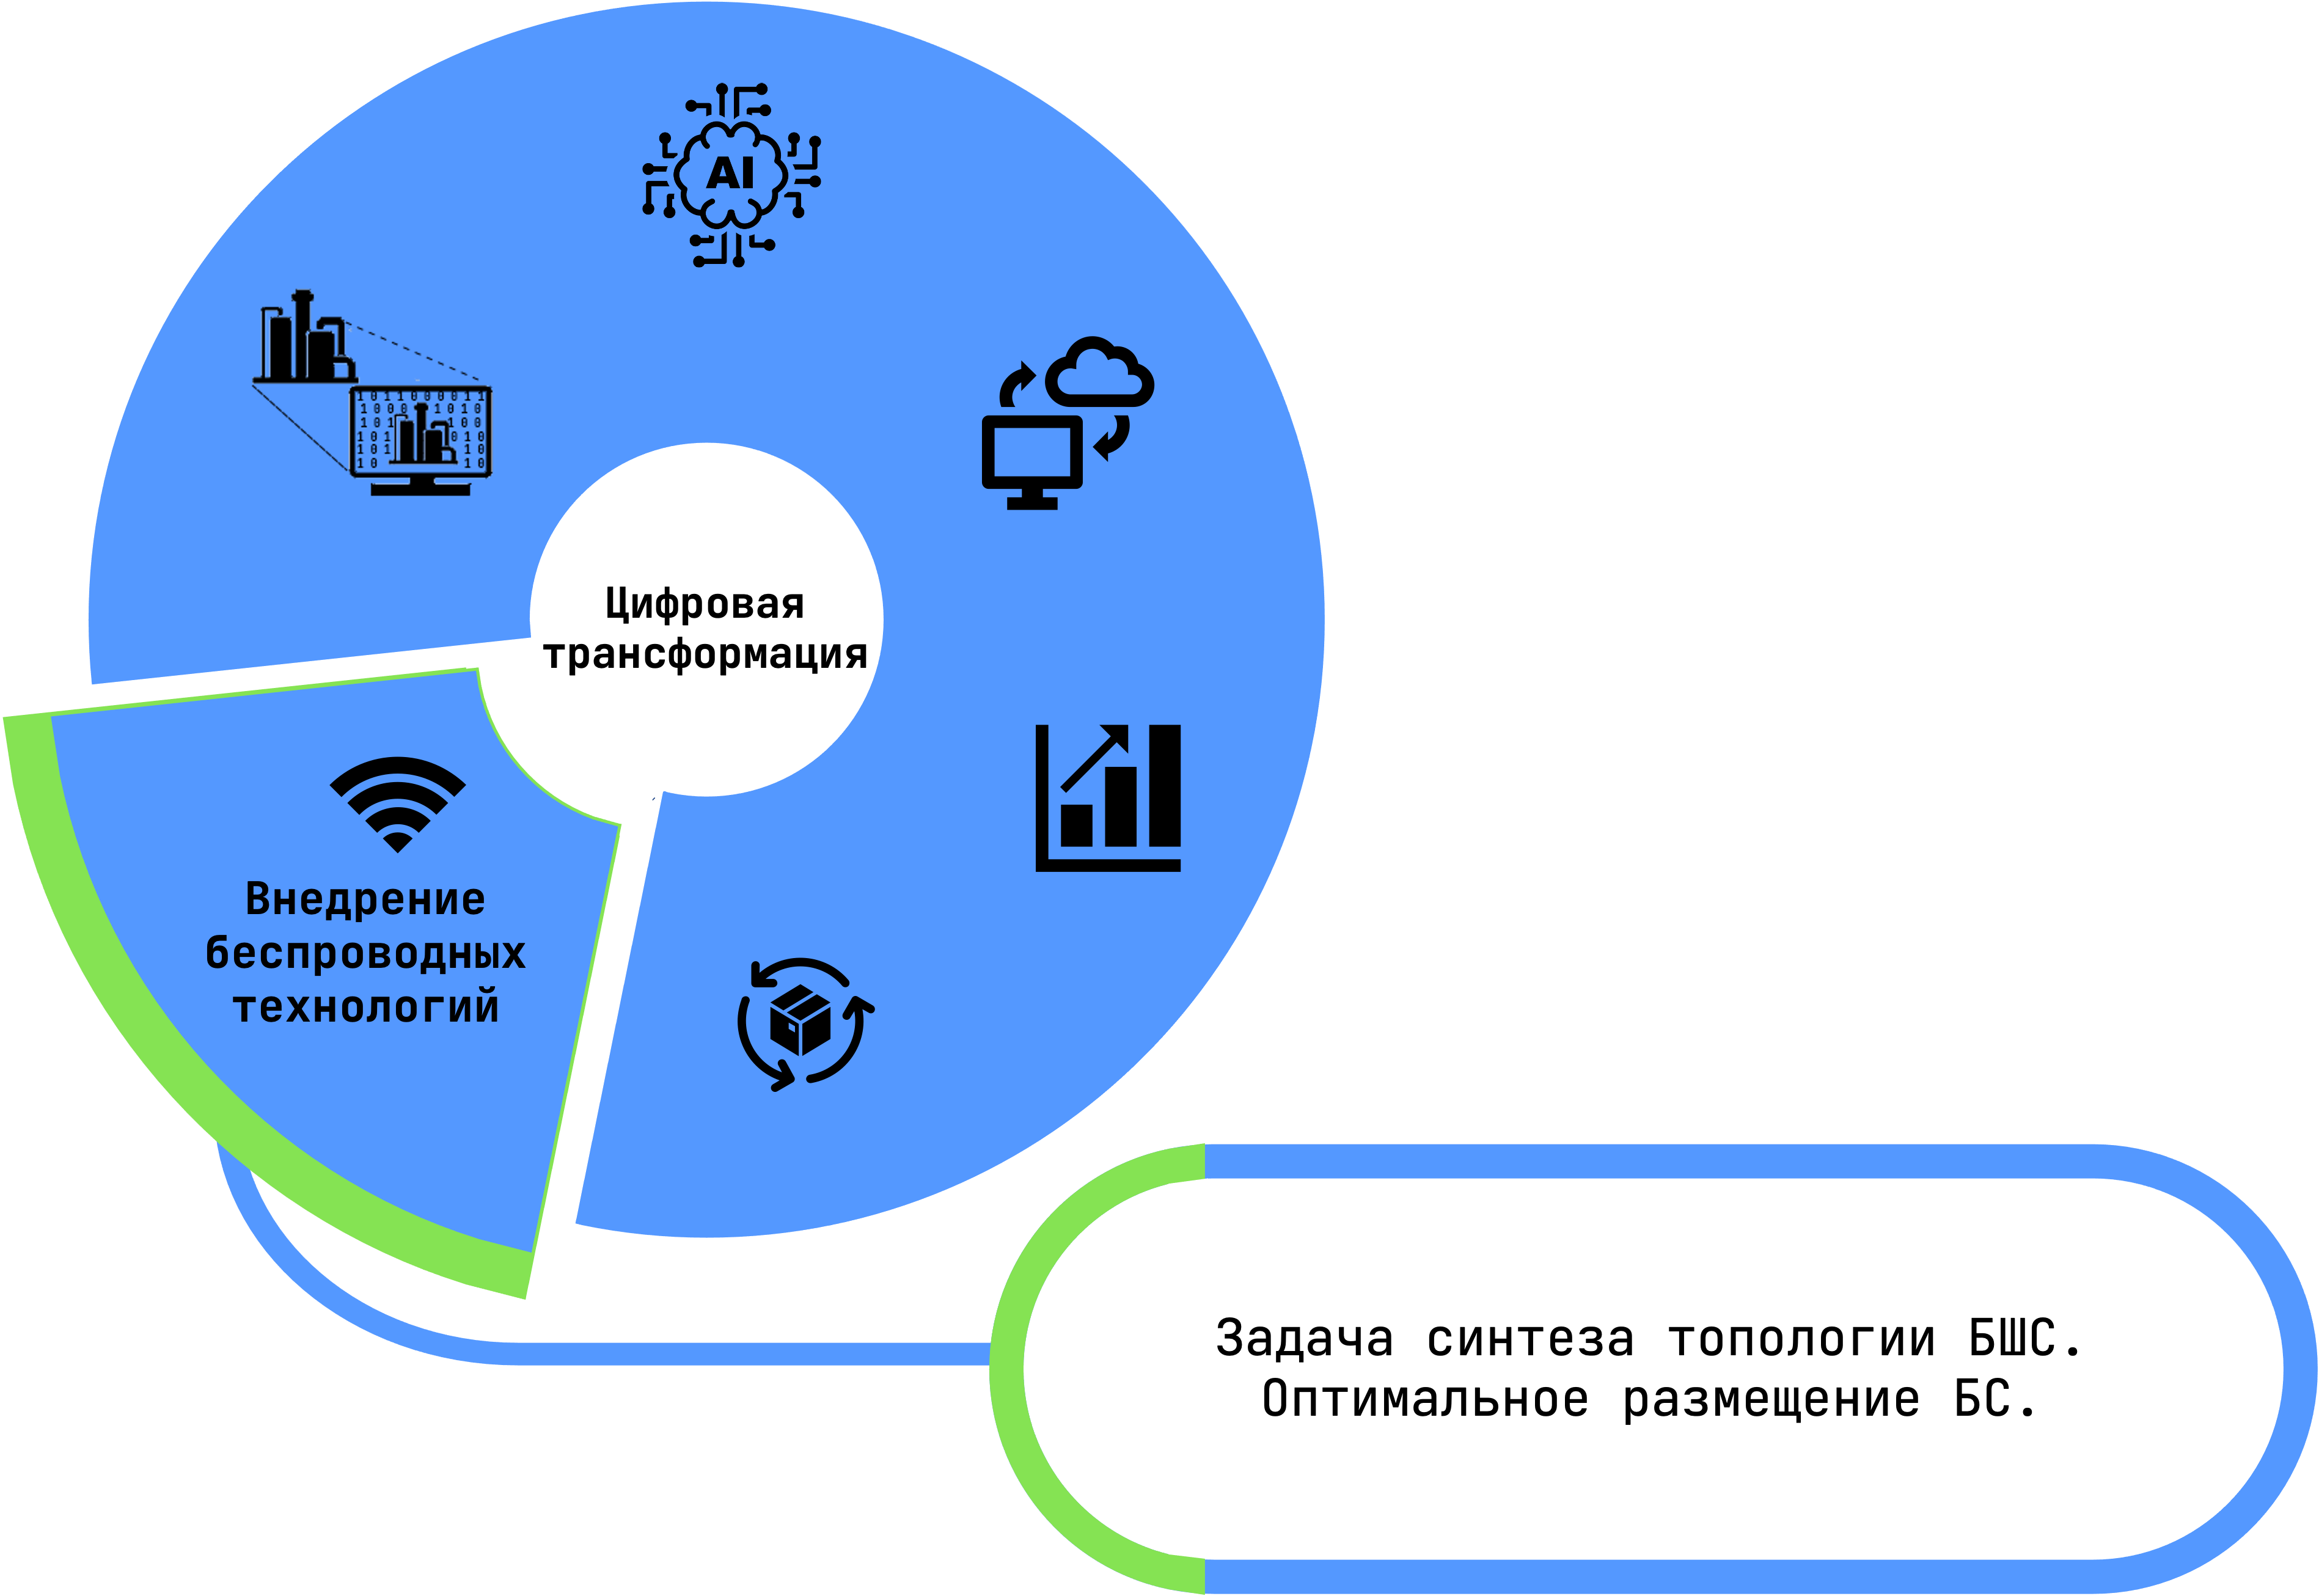
\includegraphics[width=1\textwidth]{industry4.png}
\caption{Задача синтеза топологии при проектировании БШС в рамках цифровой трансформации "Индустрия 4.0".}
\label{fig:industry4}
\end{figure}






\section{\fixme{Анализ современных беспроводных широкополосных технологий передачи данных}}

\begin{itemize}
  \item сенсорные сети
  \item беспроводная передача 
\end{itemize}

\fixme{
  IEEE 802.15.4 standard like WirelessHART, ISA100.11a,
  or ZigBee [5], [6] are popular choices for industrial wireless
  communication. The use of Bluetooth [7] or DECT [8] is
  common as well. IEEE Std 802.11, known as Wi-Fi, is also
  used on factory floors. 
}

\begin{itemize}
  \item ZigBee;
  \item Bluetooth;
  \item WirelessHART;
  \item ISA 100 Wireless
  \item Wi-Fi;
  \item WiMax;
  \item найти информацию про LoRA
\end{itemize}

\subsection{Ячеистые сенсорные сети}
Нижний уровень АСУ ТП, включающий измерительные приборы технологических параметров, исполнительные механизмы, коммутируемые с устройствами сопряжения, объединяются в беспроводную сенсорную сеть для эффективного мониторинга, контроля и управления технологическим объектом \cite{Florencio2020}.


Ячеистая сеть (Mesh) является одной эффективных технологий, позволяющая работать в неблагоприятных климатических условиях \cite{Sidney2015} \fixme{Добавить обзор}. Ячеистые сети имеют повышенную надежность благодаря тому, что каждое устройство является узлом такой сети, через который помимо сигнал с самого устройства передается сигнал смежных узлов сети.
Сеть на основе ячеистой топологии надежна, энергоэффективна. Высокая надежность обеспечивается наличием резервных маршрутов передачи данных. При прекращении функционирования одного из устройств (датчиков), передача сигнала будет происходить в обход устройства, по резервному пути. Ключевым недостатком MESH сетей является -- низкая скорость передачи данных. К ключевым преимуществом сенсорных сетей можно также отнести автономность питания, позволяющее установку узлов (устройств) сети на удалении от проводных сетей и общего питания. 


Благодаря невысокому энергопотреблению устройств ячеистые сенсорные сети могут работать продолжительное время от одного элемента питания. Это осуществляется за счет управления временем опроса данных в диапазоне от одной секунды до одного часа. Такой подход позволяет  экономить заряд батареи устройства и увеличивает продолжительность жизни устройства.

\subsubsection{ISA 100.11a}
Данный протокол является одним из распространенных протоколов передачи сигнала на промысле. Так компания Honeywell Process Solutions приняла решение разрабатывает оборудование, совместимое с ISA 100 Wireless \cite{Sidney2015}.
Топология, используемая в ISA 100.11a, основана на соединении типа "точка -- точка". Такая сеть представляет собой централизованную систему, где каждое полевое устройство связано непосредственно с главным устройством (шлюзом). 

Протокол ISA 100.11a определяют следующие методы: расширенный спектр со скачкообразной перестройкой частоты (FHSS), множественный доступ с временным разделением каналов (TDMA) и множественный доступ с контролем несущей (CSMA).

Как и любая MESH сеть, данная технология энергоэффективной, т.е. с меньшим энергопотреблением для мощности передачи сигнала. Данный фактор вносит существенную проблему, каждое устройство должно быть в непосредственной близости от шлюза и иметь прямую видимость для передачи данных. Для решения этой проблемы, в стандарт была добавлена поддержка Mesh. Потеря связи и плохой сигнал сказываются не только на целостности и своевременности получаемой информации, но и на жизненном цикле батареи питания \cite{Tagirov2013}.

\subsubsection{ZigBee}
Технология Zigbee основана на протоколе IEEE 802.15.4 LR PAN (Low Rate Personal Area Network) для низкоскоростных сетей с малым энергопотреблением. Этот стандарт описывает физический и канальный уровни со скоростью обмена данными до 250 Кбит/с и вариантами топологии "звезда","точка-точка" и Мesh. Частотный диапазон сети для России 2400 - 2483 МГц (16 каналов). Дальность связь -- 200 м. Стандарт поддерживает до 255 одновременно подключенных устройств. Ключевым преимуществом ZigBee является низкое энергопотребление. Исторически технологии ZigBee развивалась не в направлении повышения скорости передачи данных, а по пути улучшения алгоритмов сетевого взаимодействия для обеспечения длительного время работы без замены электропитания.  В сетях ZigBee различают два типа устройств -- полнофункциональные устройства FFD (Full-Function Device) и устройства с сокращенным набором функций  RFD (Reduced-function Device). Устройство FFD выступает в роли координатора, то есть организующего сеть и ретранслирующего сообщения. Устройства RFD не могут обмениваться данными друг с другом, а только через координатор FFD.

Сеть ZigBee строится на базе трех основных устройств: координатор, оконечное
устройство и маршрутизатор. Координатор выполняет основную роль в сети: формирует,
запускает сеть, участвует в построении сети, управляет ею, выполняет функции
маршрутизатора и доверительного центра (trust-центра) – устанавливает настройки
безопасности, задает настройки в процессе присоединения устройств к сети, управляет
ключами безопасности [3]. 

\subsubsection{WirelessHART}


Протокол WirelessHART разработан для мониторинга на базе проводного протокола HART с выходным сигналом 4 -- 20 мА. Верхний стек WirelessHART соответствует верхним уровням HART и Modbus. Первой компанией, которая предоставила оборудование, поддерживающее WirelessHART была Emerson. Технология также, как и ZigBee, соответствует стандарту IEEE 802.15.4, работающая в частотах не лицензируемого диапазона ISM (промышленность, наука и медицина) —- 2400–2483,5 МГц.

Координация коммуникации в сети c одноуровневым кодированием осуществляется посредством метода множественного доступа с временным разделением каналов (Time Division Multiple Access – TDMA), который синхронизирует радиостанции с периодом 10 мс \cite{Chupaev2018}. Шлюз системы WirelessHART поддерживает до 250 полевых устройств. 

В WiressHART используется широкополосная модуляция методом прямой последовательности DSSS. Для предотвращения интерференции с сетями, работающими на этой же частоте, предусмотрена технология скачкообразной смены несущей частоты (FHSS) \cite{Tagirov2013}

\subsubsection{LoRaWAN}
LoRaWAN -- современный стандарт интернета вещей (IoT) с большим потенциалом. Применяется для передачи низкоскоростного трафика. Данная технология только начала осваивать промышленный сектор. К преимуществам LoRaWAN относят очень высокую чувствительность приемника до -148 дБм, большая дальность связи 10-15 км и низкое энергопотребление у конечных устройств. По сравнению с другими энергоэффективными сетями LoRaWan имеет колоссальную дальность коммуникационной связи. Демодулятор LoRa может работать при входном сигнале, ниже уровня собственных шумов, вплоть до -20 дБ \cite{Yang2020}. 

Низкое энергопотребление осуществляется за счет передачу небольших пакетов данных. Это в свою очередь приводит к относительно низкой пропускной способности. Скорость передачи в зависимости от используемой технологии передачи данных на физическом уровне варьируется от нескольких сотен бит/с до нескольких десятков кбит/с.



\fixme{Почитать про LoRaWAN. Может быть подойдет под задачу на плоскости.}


\subsection{Сети дальнего радиуса действия с высокоскоростным трафиком}

Ячеистые сенсорные сети давно и прочно вошли как неотъемлемая часть АСУ ТП на производстве. Тем не менее они имеют один существенный недостаток -- малый радиус действия связи. Для решения такой проблемы, кластеры ячеистых сетей объединяет между собой в иерархическую структуру, в которой шлюзы объединяются в сети, на базе протоколов дальнего радиуса действия: Wi-Fi, WiMAX \cite{Savazzi2013}. Такие технологии организуют второй уровень, после уровня сбора и обработки информации с полевых устройств, для передачи данных в центр управления.




\subsubsection{Wi-Fi}



\fixme{Смартфоны от Honeywell}

\fixme{Рассказать про mesh 802.11s}

Организация сети для передачи мультимедийного высокоскоростного трафика с камер видеонаблюдения, а также сбор данных с мобильных устройств обслуживающего персонала \cite{Sidney2015} \fixme{Добавить обзор}.


\subsubsection{WiMAX}
Технология WiMAX основана на стандарте IEEE 802.16. Разработанный стандарт беспроводной широкополосного доступа рассчитан на внедрение в городских распределенных региональных беспроводных сетях в диапазонах до 66 ГГц. Стандарт предусматривает 5 режимов работ. Режим магистральной передачи WirelessMAN-SC работает в диапазоне 10-66 ГГц со скоростями до 120 Мбит/с и шириной канала порядка 25 МГц. Применяемые топологии -- "точка-точка" и "точка - много точек" \cite{Vishnevsky2009}. Остальные режимы WirelessMAN-SCa, WirelessMAN-OFDM, WirelessMAN-OFDMA и  WirelessHUMAN работают на частотах 2-11 Ггц. Режим WirelessMAN-OFDM поддерживает архитектуру Mesh. Дальность связи для WiMAX технологии достигает 20 км для прямой видимости и хорошего состояния радиоканала.

На сегодня технология применяется в качестве организации резервированного канала связи для сбора данных с кустовых площадок с блока местной автоматики в диспетчерский пункт и мультимедийного трафика с систем видеонаблюдения. 

Технология WiMAX успела получить свою популярность на месторождениях и занять свою нишу в организации телекоммуникационной связи. Исторически WiMAX всегда рассматривался как альтернатива сотовым сетям связи. С резким скачком популярности LTE и появлением сетей пятого поколение WiMAX давно уже является не конкурентным стандартом на рынке.





\fixme{БС организуются в сети WiMax и Wi-Fi}

\fixme{Для обеспечения связи между станциями буду использовать Wi-Fi }

При внедрении беспроводных технологий необходимо учитывать специфику выполняемых задач будущей сети. Для каждого конкретной цели существуют свои требования к скорости передачи данных, дальности связи, потребляемой мощности, помехозащищённости, надежности и т.д. Чтобы учесть специфику данных задач разработано множество беспроводных решений, охватывающее дальность связи от несколько сантиметров до десятков километров и скоростей передачи от единиц Кбит/с до сотен Мбит/с.

\fixme{Наиболее массовыми технологиями в области промышленной автомати¬зации являются Wi-Fi, Bluetooth и ZigBee [11-16], ключевые параметры которых представлены в табл. 1.1. Оборудование данных технологий рабо¬тает в нелицензируемом радиочастотном диапазоне 2,4 ГГц и не требует регистрации в государственных органах при соблюдении условий применения [17].}



\fixme{
IWN унаследовали многие функции WSN, особенно протоколы связи и промышленные приложения [91]. Однако из-за особенностей промышленной среды и того, что промышленные беспроводные сети Индустрии 4.0 отличаются от традиционных WSN [17, 37], существуют некоторые новые ограничения и требования к IWN. Основные различия между IWN и WSN перечислены ниже:}

\fixme{
IWN с задержкой используются в отраслевых системах для определения важных параметров, таких как мониторинг состояния машины и рабочей среды или предоставление команд управления и информации в реальном времени. Поэтому этим приложениям требуется низкая задержка. В большинстве случаев это происходит за счет энергопотребления и высоких затрат на достижение производительности в реальном времени. Напротив, WSN ограничены энергией, и узлы могут быть развернуты в недоступных доменах, что затрудняет замену или обновление батарей. Как следствие, необходимо максимально увеличить время автономной работы в WSN, что приведет к увеличению задержки. }

\fixme{
Мобильность Как обсуждалось выше, для повышения гибкости и мобильности для Индустрии 4.0 IWN могут содержать больше движущихся узлов, таких как мобильные продукты, мобильные роботы, автомобили с автоматическим наведением, беспилотные летательные аппараты, рабочие и другие мобильные устройства. Это контрастирует с узлами WSN, которые обычно считаются стационарными или с несколькими движущимися узлами, такими как движущийся приемник, ретрансляционные узлы и т. Д.
}

\fixme{Среды Еще одно существенное различие между IWN и WSN - это операционная среда. Во-первых, в промышленной сфере IWN работают в сложных условиях из-за пыли, вибрации, тепла, различных препятствий, а также более высокой температуры и влажности. Во-вторых, существуют более серьезные помехи сигналам от двигателей и других беспроводных сетей, чем для традиционных WSN. Кроме того, промышленная среда может легко повлиять на радиоканал, который отличается от WSN. Следовательно, IWN нуждаются в дополнительных стратегиях, чтобы гарантировать надежность и эффективную связь. Напротив, узлы WSN развернуты в относительно стабильной и дружественной среде.}


% \fixme{Производительность Для Индустрии 4.0 все оборудование, устройства, рабочие, терминалы и другие узлы могут выполнять сложные задачи индивидуально и взаимодействовать с другим оборудованием. Специально для IWN узлы не только обмениваются данными со своими соседями для выполнения механических задач, таких как перемещение, закрепление и транспортировка, но также должны справляться с такими проблемами, как помехи сигнала, пути перемещения и обработка данных. Как следствие, с точки зрения пропускной способности узлов, узлам IWN требуются более высокие мощности для обработки данных, энергии и хранения, и они более умны, чем традиционные узлы WSN.}

Говоря простым языком инженеров - разработчиков, аббревиатурой LoRa (Long Range) обозначают лишь вид модуляции, то есть уровень l1 по модели OSI.
А имя LoRaWAN носит Протокол канального уровня.
Преимущества LoRa:
- использует частотный диапазон, разрешенный для использования в России;
- разрабатывалась для работы на мощности 25 мВт;
- это открытый стандарт, и чипы для конечных устройств имеются в свободной продаже;
- имеет хороший радиус действия даже в городской среде 3 км, до 20 км радиус покрытия базовой станции вне городской застройки;
- от 1 батарейки датчики LoRa могут запитываться не менее 1 года;
- базовые станции LoRa, подключенные к одному сетевому серверу, работают как единый механизм;
- LoRaWAN-сеть ЭР-Телекома зарегистрирована в едином списке сетей операторского класса и имеет международный NetID - 52, обеспечивающего возможность предоставлять роуминг;
- дополнительное шифрование данных на основе платформы приложений.


\section{Этапы проектирования БШС}

Для обеспечения высокого качества беспроводной связи необходимо проводить грамотное проектирование БШС. Существуют различные подходы к проектированию беспроводных сетей. Для одних задачей является максимальная зона покрытия, для других -- достижения максимальной производительности передачи данных, для третьих -- нахождения баланса между зоной охвата и производительностью \cite{Proletarsky}. В диссертации будут предложены модели и методы оптимального размещения базовых станций (БС) БШС, целью которых является максимальная зона охвата.  Процесс проектирования современной БШС, как правило, для такого подхода имеет следующие основные этапы (Рисунок \cref{fig:part1_design_stages}):

\begin{figure}[h!]
  \centering
   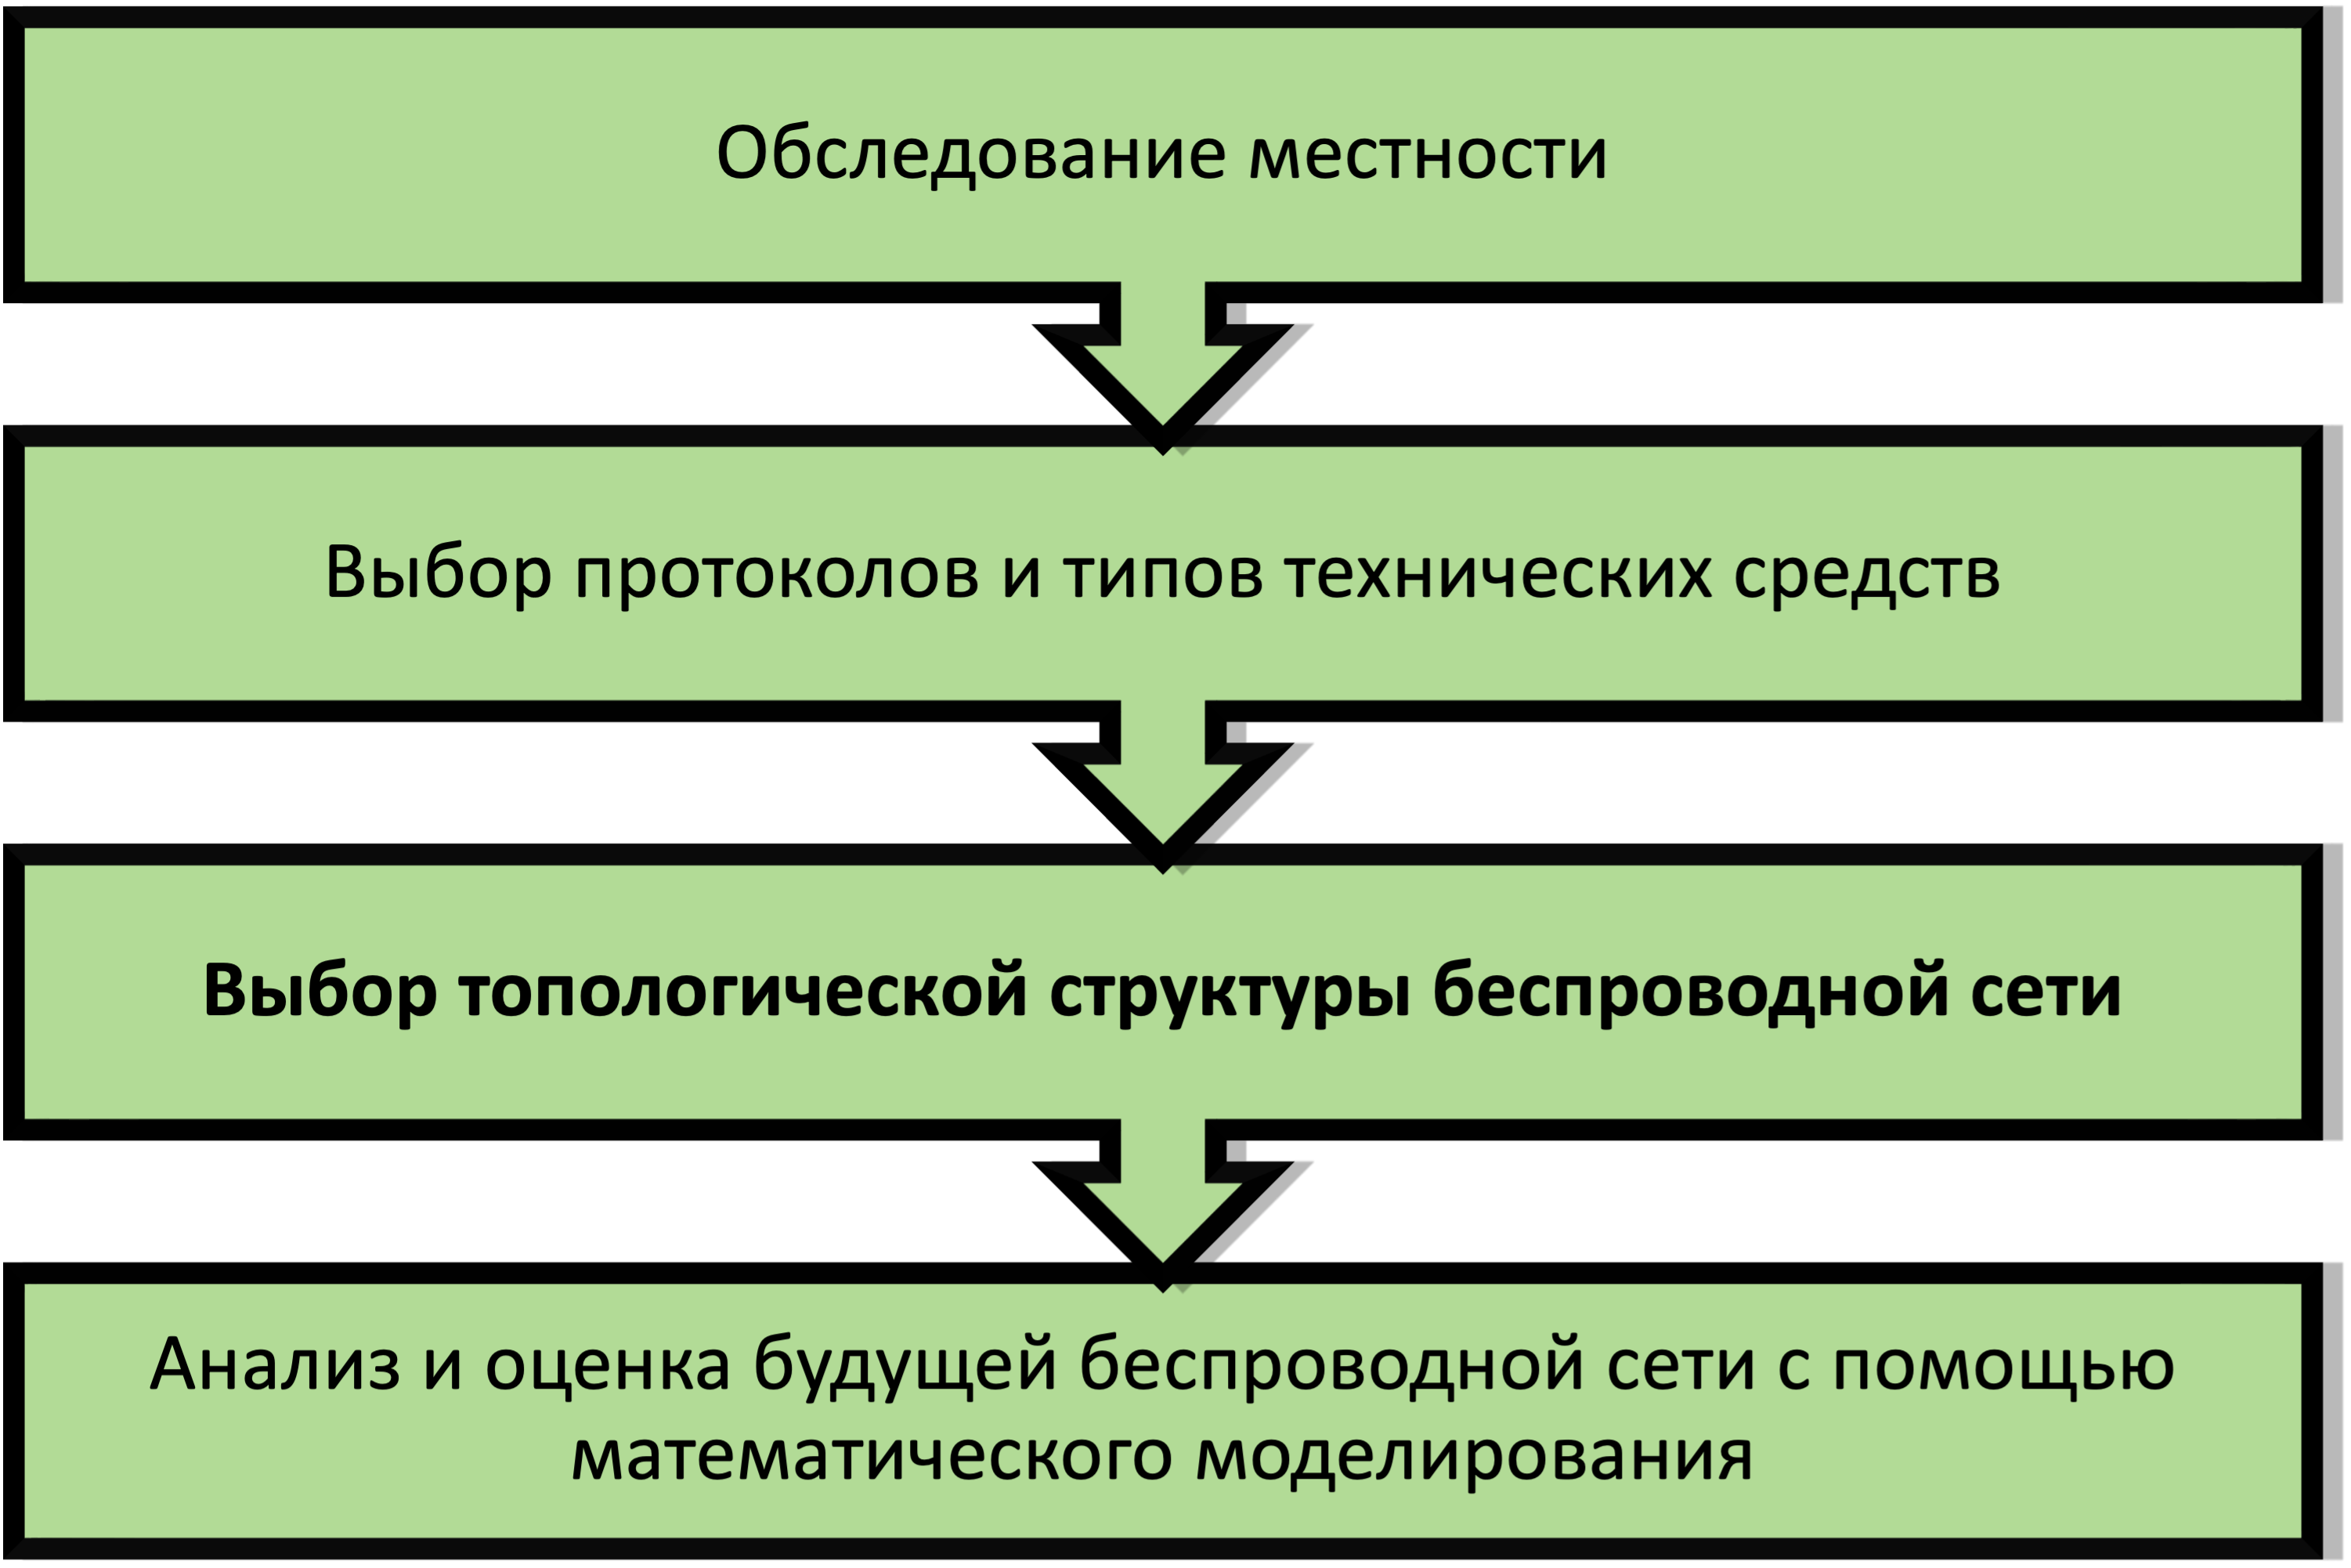
\includegraphics[width=0.8\textwidth]{design_stages.png}
\caption{Этапы проектирования БШС.}
\label{fig:part1_design_stages}
\end{figure}

Любое проектирование БШС всегда начинается с первоначального обследования местности. В данный этап входят задачи радиобследования и радиопланирования. оценки реальных размеров области контроля, наличие стационарных инженерно-технических соооружений, мешающих передачи сигнала, такими как металлические конструкции, перекрытия, стены и т.д. При развертывании БШС в открытой местности также немаловажную роль играет наличие перепада высот. В ходе выполнения комплекса работ на местности, определяются возможные точки размещения оборудования \cite{Dunaitsev2017}. На основе результатов данного этапа проводится выбор типо моделй оборудования для дальнейшего их размещения и организации сети.

Производительность и дальность действия беспроводных сетей не безграничны. При их проектировании стоит учитывать множество параметров: частота, скорость, мощность излучения \cite{Proletarsky}. На этапе выбора оборудования необходимо определиться с протоколом будущей БШС и  подготовить необходимый комплекс технических средств для развертывания будущей сети. БС является основопологающим устройством будущей сети, которая отвечает за покрытие задданной области. Покрытие в свою очередь зависит от мощности передатчика устройства, усиления антенн, чувствительности приемного устройства.


После определения множества возможных точек размещения БС на этапе обследования местности и выборе возможных типов и моделей оборудований можно переходить непосредственно к размещению БС и определению топологической структуры сети. Этап выбора топологической структуры будущей сети является ключевой проблемой данной диссертации. В рамках данной проблемы будут предложены модели и методы оптимального размещения БС для организации БШС.

После решения задачи синтеза топологии, для полученного размещения решаются задачи оценки характеристик производительности БШС. Для расчета оценок широко применяется аппарат теории массового осблуживания (ТМО). Примерами таких задач являются расчет надежности всех элементов сети \cite{Wankpo2020, Krishnamoorthy2021, Kozyrev2019}, оценка характеристик качества канала, вероятности потери пакетов, пропускной способности, времени доставки сообщений в сети \cite{Gorbunova2020, Larionov2019, Vishnevsky2016_Methods_of_performance, Vishnevsky2016_Review_of_methodology, Wang2017, Sandmann2012, Baumann2017}, оценка межкоцневой задержки сети \cite{Wang2017, Sandmann2012}. В работе \cite{Eremenko2013} рассматривают стохастическую модель марковской цепи для оценки качества предоставления информационных услуг передачи данных автоматизации систем управления технологическим процессов (АСУ ТП) в условиях помех и прерываний. Одним из современных направленией в исследовании характеристик производительности БШС является использование ТМО в совокупности с методами машинного обучения (МО) \cite{Lovas2021, SatyaHermanto2018}.

Описанная процедура проектиррования БШС является общей для большинства внедрения беспроводных коммуникационных сетей. В зависимости от конкретных целей, которые преследуют проектировщики, план работ может требовать содержание конкретных этапов и подзадач проектирования. В общем же случае проектирование БШС будет происходить согласно данной последовательности этапов. В изложенной концепции важным является представление места результатов исследования данной диссертации в глобальной задаче комплексного проектирования.

\section{Определение расчетных параметров БШС, необходимых для решения задач размещения базовых станций}

Этап выбора топологической структуры беспроводной сети состоит из решения задач оптимального размещения БС. В дальнейшем для решения данных задач необходимо будет ввести параметры БС: радиус связи -- максимальная теоретическая дальность связи базовой станции с соседней станцией, удовлетворящей требуемому качеству передачи сигнала; и радиус покрытия -- максимальный теоретический радиус зоны покрытия БС для связи с устройствами. Данные параметры рассчитываются исходя из конфигурации БС. Далее будет представлен метод расчета. Все технческие харакетеритики для расчета берутся из технического паспорта БС.

% \subsection{Расчет дальности связи}


% \fixme{Перед тем как приступить к задаче ЦЛП необходимо рассчитать характеристики станции: радиус связи $R_{jq}$ и радиус покрытия $r_j$.}

% \fixme{При развертывания сети необходимо обеспечить максимальное покрытие данного участка связь между шлюзами через систему размещенных базовых станций беспроводной широкополосной сети}.
В БШС в большинстве случаев используются радиоволны сантиметрового диапазона. Отличительной чертой распространения данных радиоволн  является почти полное отсутствие явления дифракции и прямолинейность распространения. Волны практически не огибают преград при распространении, поэтому существенное влияние оказывают рельеф местности, преграды и погодные условия. 

Для расчета дальности действия связи используют модели распространения радиосигнала \cite{ElChall2019, Zhang2021, Caso2015, Kang2020}.Существуют различные модели, которые можно объединить в три основные категории \cite{Oni2017}:
  \begin{itemize}
    \item теоретические модели. Данные модели обычно основана на физическом предположении об идеальных условиях;
    \item эмпирические модели. Это наборы уравнений, разработанные на основе различных данных полевых измерений. Одним из основных недостатков таких моделей является то, что они не могут использоваться для различных ситуации без изменений, поскольку они точны только для случая с теми же характеристиками, в которых проводились измерения;
    \item детерминированные модели. Модели очень сложны, поскольку они требуют детального знания местоположения, размеров и физических параметров всех препятствий в данной области.Такое детальное исследование может приводить к чрезмерным накладным расходам, которые в большинстве случаев могут быть лишними.
  \end{itemize}

Существуют большое количество моделей распространения. Каждая имеет свои плюсы и минусы. В зависимости от конкретных задач при проектировании возможно использовать каждую из них. \fixme{В данном исслeдовании используется простейшая модель распространения в свободном пространстве (Free space propagation model).}

\subsection{Энергетический потенциал канала связи}
Для оценки производительности канала связи используется уравнение энергетического потенциала, который учитывает все усиления и потери уровня сигнала при его распространении от передатчика к приемнику через беспроводную  среду передачи, кабели, разъемы, различные препятствия (Рисунок \cref{fig:link_power}) \cite{Proletarsky}.

В определении энергетического потенциала беспроводной линии связи участвуют следующие параметры:
\begin{itemize}
  \item эффективная изотропно-излучаемая мощность передатчика (Equivalent Isotropically Radiated Power, EIRP), являющаяся суммой выходной мощности передатчика и коэффциента усиления антенны за вычетом потерь в антенном кабеле разъемах передающего тракта;
  \item потери пр распротранении в свободном протранстве;
  \item чувствительность приемника, потери в антенном кабеле и коэффициент усиления антенны приемника.
\end{itemize}
Полное уравнение можно записать следующим образом:

% It is essential during deployment to provide maximum coverage of a given area and ensure communication between the placed base stations in the wireless broadband network. 

% Link Budget is a way of estimation of communication link's performance while accounting for the system's power, gains, and losses for both the transmitter and receiver. The complete equation can be written as follows:

\begin{equation}
  \label{eq:part3_link_budget}
  P_{tr} - L_{tr} + G_{tr} - L_{fs} + G_{recv} - L_{recv} = SOM + P_{recv},
\end{equation}
где:

\begin{itemize}

  \item $P_{tr}$ -- мощность передатчика, дБм;

  \item $L_{tr}$ -- потери сигнала на антенном кабеле и разъемах передающего тракта, дБ;

  \item $G_{tr}$ -- усиление антенны передатчика, дБ;

  \item $L_{fs}$ -- потери в свободном пространстве, дБ;

  \item $G_{recv}$ -- усиление антенны приемника, дБ;

  \item $L_{recv}$ -- потери сигнала на антенном кабеле и разъемах приемного тракта, дБ;

  \item $P_{recv}$ -- чувствительность приемника, дБм;
  
  \item $SOM$ -- запас на замирание сигнала, дБ.

\end{itemize}
Энергетический потенциал указывает на качество канала передачи радиосигналов.

\begin{figure}[h!]
  \centering
   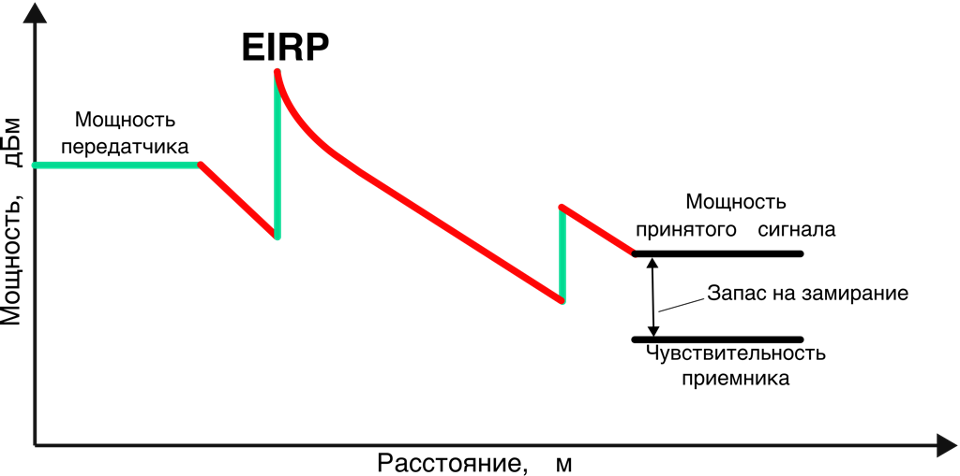
\includegraphics[width=1\textwidth]{link_power.png}
\caption{Энергетический потенциал линии связи.}
\label{fig:link_power}
\end{figure}

На стороне передатчика выходной мощностью является величина, равная мощности, подводимой к антенне. Данная величина из паспортной документации устройства имеет различные значения в зависимости от каждого поддерживаемого оборудованием стандарта и конкретных скоростей. В реальной условиях значения мощностей, как правило могут незначительно отклоняться от паспортных значений. Предельная мощность передатчика определяется государственными органами. Для примера, для БШС семейства протоколов IEEE 802.11 не превышает 100 мВт или, выражая в децибеллах, не боллее 20 дБм \cite{GKRCh18_13}.


Затухание сигнала могут происходить в кабелях антенны, зависящие от типа кабеля и рабочей частоты. При подключении антенны желательно обходиться минимальной длиной кабеля. Потери сигнала в антенном кабеле принимают $0, 1...2$ дБ/м. В технической документации в потерях кабеля также учтена величина затухания в кабельных разъемах. 

Усиление антенны описывает фокусирование переданного или полученного сигнала. Значения даны относительно полуволнового диполя или теоретического изотропного излучателя \cite{Gost62657}.

Мощность принимаемой антенны рассчитывается из уравнения передачи Фрииса:

\begin{equation}
  \label{eq:part1_Friis}
  \frac{P_{recv}}{P_{tr}} = G_{tr}G_{recv}\left(\frac{c}{4\pi R f} \right)^2,
\end{equation}
где
$c$ --  скорость света,
$f$ -- частота, 
$R$ расстояние между приемной и передающей антенной.


К потерям при распространении относятся все виды затухания сигнала, которые имеют место при его распространении от антенны передатчика к антенне приемника. Самая простая оценка потерь в свободном пространстве получается, если предположить, что сигналы передаются во всех направлениях, то есть мощность излучается одинаково во всех направлениях, и в зоне передачи или вокруг нее нет препятствий, которые могли бы повлиять на распространение электромагнитных сигналов \cite{Krouk2010}. Передающий сигнал рассеивается по мере увеличиня расстояния между приемником и передатчиком. Данный тип затухания называется потерями в свободном пространстве (Free Space Path Loss, $FSPL$).

\subsection{Модель потерь в свободном пространстве}
При распространении сигнала от передатчика к приемнику часть сигнала рассеивается, по этой причине мощность на приемной стороне будет уменьшаться с увеличением  расстоянии от передающей антенны. Данное затухание сигнала называют потерями в свободном пространстве.

Потери при распространении между двумя неизотропными антеннами в свободном пространстве (в воздухе) можно выразить из уравнения Фрииса \cref{eq:part1_Friis}:

% \begin{equation}
%   \label{eq:part3_FSPL}
%   FSPL = \left(\frac{4\pi R f}{c} \right)^2.
% \end{equation}

% Формула \cref{eq:part3_FSPL}, выраженная в децибеллах будет выражаться как

\begin{equation}
  \label{eq:part3_L_fs}
  L_{fs} = 20 \lg{F} + 20\lg{R} - G_{tr} - G_{recv} + K,
  \end{equation}
где $F$ -- центральная частота, на котором работает канал связи, $R$ -- расстояние между приемной и передающей антенной и $K$ -- константа.

Константа $K$ зависит от размерностей частоты и расстояния:

\begin{itemize}
  \item для частоты, выраженной в ГГц, и расстояния, выраженная в км, константа $K$ равна 92.45;
  \item для частоты, выраженной в МГц, и расстояния, выраженная в км, константа $K$ равна 32.4;
  \item для частоты, выраженной в МГц, и расстояния, выраженная в м, константа $K$ равна -27.55.
\end{itemize} 

Потери $L_{fs}$ выразим из уравнения энергетического потенциала канала связи \cref{eq:part3_link_budget} как:

\begin{equation}
  \label{eq:part3_L_fs_from_link_budget}
  L_{fs} = P_{tr} - L_{tr} + G_{tr} + G_{recv} - L_{recv} - SOM - P_{recv}.
\end{equation}


Запас на замирание сигнала, SOM,  учитывает все возможные факторы отрицательно влияющие на дальность связи. К таким факторам относятся:

\begin{itemize}
  \item температурный дрейф чувствительности приемника и выходной мощности передатчика;
  \item влияние погодных условий на передачу сигнала: туман, снег, дождь;
  \item  потери в антенно-фидерном тракте, возникающие из-за рассогласования фидера и антенны.
\end{itemize}
Приемник испытывает совокупное воздействие всех этих физических факторов, которые различаются в зависимости от положения приемника и передатчика в среде распространения. 

Минимальная значения величины запаса на замирание  (System Operating Margin, $SOM$) должна быть не меньше  10 дБ. Считается, что 10-ти децибельный запас по усилению достаточен для инженерного расчета, но на практике зачастую используют значение $20 ... 30$ дБ \cite{Proletarsky}.

% \fixme{Энергетический потенциал указывает на качество канала передачи радиосигналов}.



% The Free Space Path Loss ($ FSPL $) equation defines the propagation signal loss between two antennas through free space (air):



Максимально возможную дальность связи между приемником и передатчиком выводится из уравнений \cref{eq:part3_L_fs} и \cref{eq:part3_L_fs_from_link_budget}:

\begin{equation}
  \label{eq:part3_D}
  R = 10^\frac{L_{fs} - 20\lg{F} + G_{tr} + G_{recv} - K}{20}.
\end{equation}

Используя формулу \cref{eq:part3_D} и \cref{eq:part3_L_fs_from_link_budget}, мы можем расчитать теоретическое максимальную дальность связи $ R_{jq}$ между базовыми станциями и радиусом покрытия $ r_j $ с предположением об отсутствии препятствий, отражений, влияния контуров местности и т. д. Это допущение приемлемо для нашего случая с открытой местностью.

\begin{figure}[h!]
  \centering
   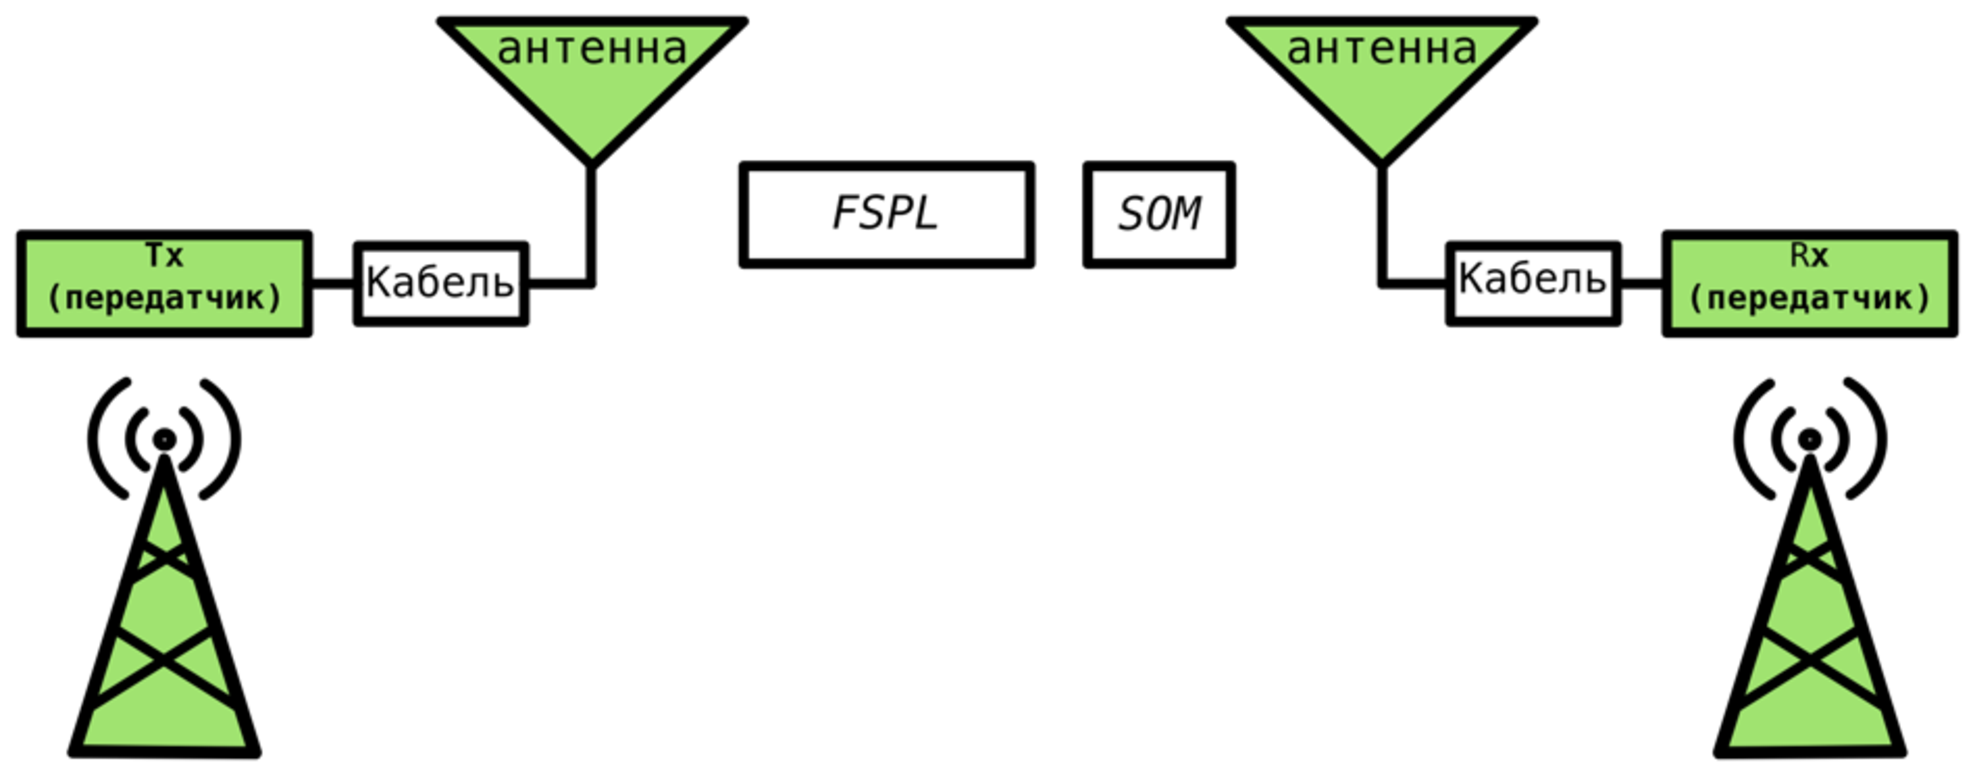
\includegraphics[width=0.8\textwidth]{link_distance.pdf}
\caption{Соединение между станциями.}
\label{fig:part3_link_distance}
\end{figure}

Для расчета дальности связи $R_{jq}$ (Рисунок \cref{fig:part3_link_distance}), базовые станции $s_j$ и $s_q$ будут рассматриваться как станции \textit{передатчик} и \textit{приемник}, соответственно. Будем считать, что станции оборудованы направленными антеннами с усилениями $G_{tr}^{R}$ и $G_{recv}^{R}$.

\begin{figure}[h!]
  \centering
   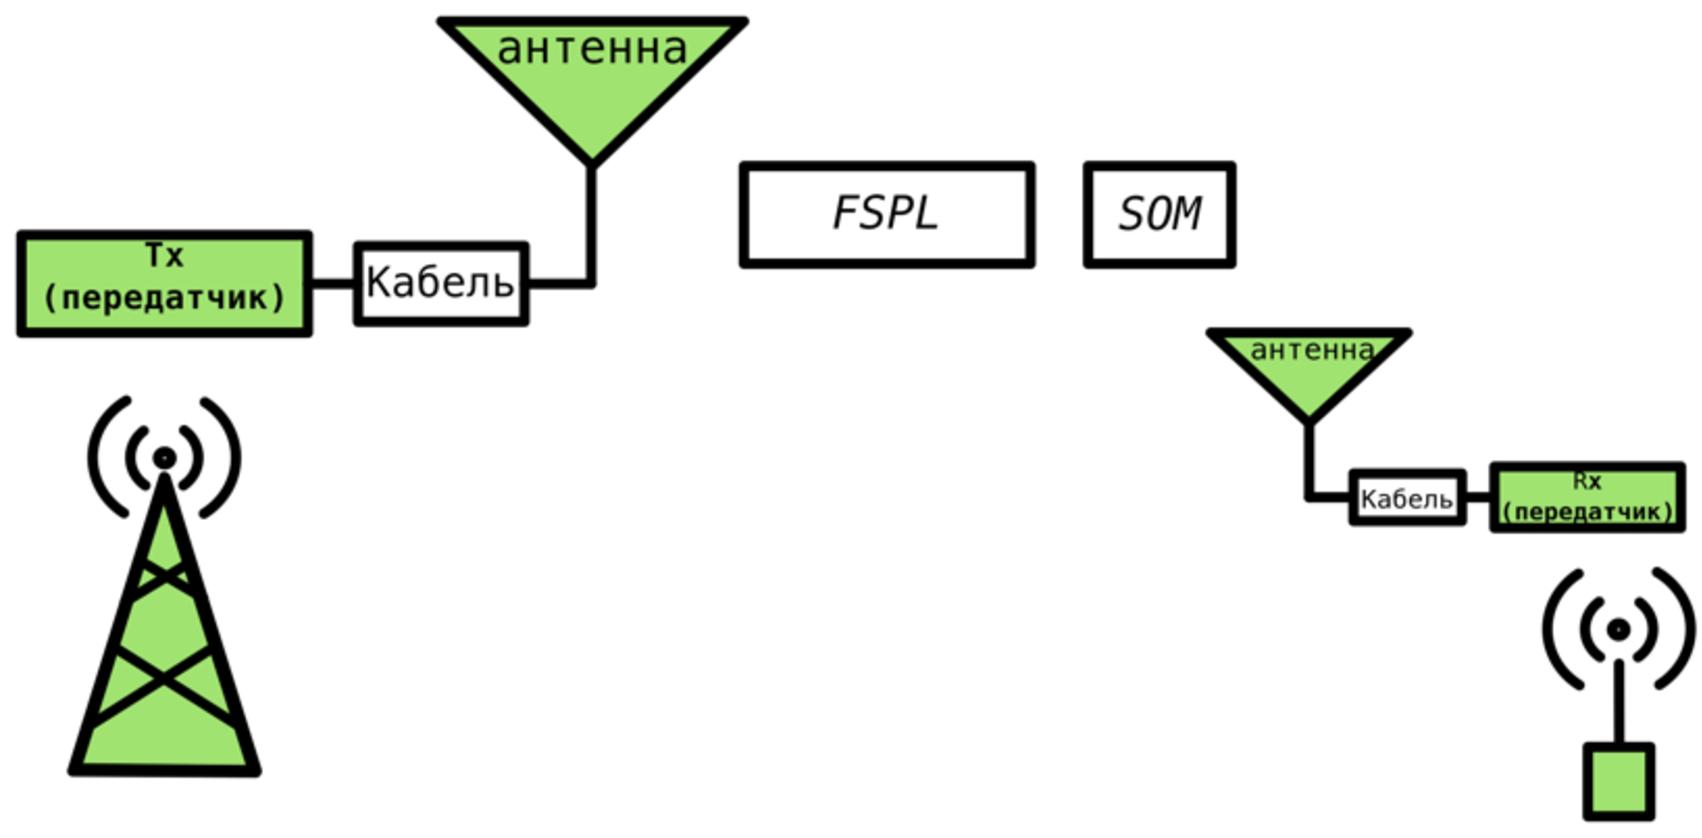
\includegraphics[width=0.8\textwidth]{coverage.pdf}
\caption{Покрытие станции}
\label{fig:part3_coverage}
\end{figure}

Каждая базовая станция оснащена всенаправленной антенной с заданным усилением антенны $G_ {tr}^{r}$. Данная антенн необходимо для покрытия заданной области.

% Each base station is equipped with an omnidirectional antenna with given gain antenna $G_{tr}^{r}$. A station uses this antenna to cover a given area.

При вычислении радиуса покрытия $r_j$ (Рисунок  \cref{fig:part3_coverage}) базовая станция будем считать \textit{передатчиком}, а пользовательское устройство \textit{приемником}.

\subsection{Модель распространения SUI}

Модель распространения SUI (Stanford University Intern) предложена рабочей группой, занимающаяся исследованием беспроводной широкополосной сети IEEE 802.16 \cite{Mollel2014}. Модель включена в стандарты IEEE и широко используется в WiMax, а также в LTE \cite{Zreikat2017}. Подходит для использования в сельской местности с различным типом рельефа, а также в небольших населенных пунктах. Модель испытана на равнинах, пересеченной, холмистой местности и лесных массивах. SUI модель используется для диапазона частот 1900 МГц -- 11 Ггц \cite{Cabuk2020}. Высоты антенн БС в диапазоне от 10 до 80 м, высота антенны мобильного устройства –- от 2 до 10 м, расстояние между БС и устройством от 0,1 до 8 км.

Грубая оценка потери сигнал описывается с помощью модели SUI как

\begin{equation}
  \label{eq:part1_sui_l0}
  L_0 = A + 10\gamma\lg{(R/R_0)},
\end{equation}
$$
A = 20\lg{(\frac{4\pi R_0 }{\lambda})}
$$
и
$$
\gamma = a - b h_t + \frac{c}{h_t}, 
$$
где $R$ -- дальность связи, $R_0$ -- минимальная разрешенная дальность (100 м), $\lambda = c / f$ -- длина волны, $f$ -- частота в МГц, $h_t$ -- высота антенны БС, $h_r$ -- высоты антенны устройства. Параметры $a, b$ и $c$, определяющие следующие типы местности (Таблица \cref{tab:part1_abc_sui_model}):
\begin{itemize}
  \item тип A -- холмистая местность или густые лесные массивы;
  \item тип B -- пересеченная местность или полугустые лесные массивы;
  \item тип C -- открытые поля.
\end{itemize}


\begin{longtable}[c]{| c | c | c | c |}
  \caption{Численные значения параметров модели SUI.}\label{tab:part1_abc_sui_model}\\

  \hline
  \textbf{Параметры модели} & \textbf{Местность A} & \textbf{Местность B} &  \textbf{Местность C}\\ \hline
  a & 4,6 & 4 & 3.6 \\
  b & 0,0075 & 0,0065 & 0.005 \\
  c & 12,6 & 17,1 &20 \\
  \hline
  \hline
\end{longtable}




\fixme{ДОДЕЛАТЬ SUI И ДОБАВИТЬ ДВУХЛУЧЕВУЮ}

Формула \cref{eq:part1_sui_l0} была получена эмпирически для несущей частоты 2 ГГц и высоты приемника 2 м. Для использования модели с другими частотами и высотами необходимо добавить поправочные коэффициенты 

\begin{equation}
  \label{eq:part1_sui_lfs}
  L_{fs} = L_0 + \Delta L_f + \Delta L_h + s,
\end{equation}
где $\Delta L_f$ -- корректирующий коэффициент для частот свыше 2 ГГц $\Delta L_h$ --  корректирующий фактор высоты антенны устройства (м) $s$ -- корректирующий фактор теневого эффекта, имеющий значения в диапазоне $8,2 < S < 10,6$ дБ. Параметр $\Delta L_f$ рассчитывается 
$$
\Delta L_f  = 6 \lg{(f / 2000)},
$$
параметр $\Delta L_h$ выбирается исходя из выбора типа местности

$$
\Delta L_h =  
 \begin{cases}
  -10,8 \lg{(h_r/2)} &\text{для типа A и B,}\\
  -20 \lg{(h_r/2)} &\text{для типа C.}
 \end{cases}
$$

Из уравнений \cref{eq:part1_sui_l0, eq:part1_sui_lfs} можно вывести дальность действия связи:

\begin{equation}
  R = 10^{(\frac{L_{fs} - L_0 - \Delta L_f - \Delta L_h - s - A}{10\gamma} + \lg{R_0})}
\end{equation}

\subsection{Модель двух лучевого распространения}

Двух лучевая модель описывает мощность принятого сигнала как интерференцию двух копий переданного сигнала: первая -- луч прямой видимости, вторая -- отраженная от поверхности \cite{Gaitan2020}. 
Два луча электромагнитных волн от передатчика приходят в приемник с определенной разностью фаз и амплитуд. Разность фаз происходит из-за дополнительного времени распространения волны, отраженного от земли \cite{Rademacher2016, Bacco2014, Zochmann2017, Kurt2017}. 

\fixme{Проверить}

Мощность принимаемого сигнала, в соответствии с двухлучевой моделью равна

\begin{equation}
  \label{eq:part1_two-ray_model_prcev}
  P_{recv} = \frac{P_{tr} \cdot G_{tr} \cdot G_{recv} \cdot h^2_{tr} \cdot h^2_{recv}}{R^4},
\end{equation}
где $P_{recv}$ -- чувствительность приемника, $P_{tr}$ -- мощность передатчика,$G_{tr}$ -- усиление антенны передатчика, $G_{recv}$ -- усиление антенны приемника, $h_{tr}$ -- высота передатчика, $h_{recv}$ -- высота приемника, $R$ -- расстояние между приемником и передатчиком.

Потери в свободном пространстве из формулы \cref{eq:part1_two-ray_model_prcev} вычисляются как:

\begin{equation}
  \label{eq:part1_two-ray_model_lfs}
  L_{fs} = 40\lg{R} - 10\lg{G_{tr}} - 10\lg{G_{recv}} - 20\lg{h_{tr}} - 20\lg{h_{recv}},
\end{equation}

Тогда из формулы \cref{eq:part1_two-ray_model_lfs} дальность рассчитывается как:


\fixme{ПЕРЕДЕЛАТЬ ФОРМУЛУ ФРИИСА, ЧТОБЫ УЧИТЫВАТЬ НЕИЗОТРОПНЫЕ АНТЕННЫ}

\fixme{ВЕЗДЕ ПРОВЕРИТЬ ЛОГАРИФМ ПО ОСНОВАНИЮ 10}

\subsection{\fixme{Расчет параметров БС, необходимых для задач оптимизации}}

\section{Оценка характеристик производительности сети с помощью стохастических моделей массового обслуживания}

\subsection{\fixme{Время передачи пакета в канале}}

\subsection{Расчет межконцевой задержки}\label{part4_e2e_delay_section}

Как уже было отмечено ранее, одним из важных ключевых задач при проектировании БШС является оценка ее характеристик производительности для удовлетворения требуемого качества обслуживания (quality of service, QoS). Одной из основных характеристик проектируемой сети является ее межконцевая задержка \cite{Vishnevsky2016_Methods_of_performance, Wang2017, Liu2016, Chen2019, Hosni2017, Capone2019, Abbas2017, Seliem2019, Malandra2018, Kalor2018, Larionov2019, Gao2016}. Для расчета сквозной задержки сети используют стохастические модели массового обслуживания \cite{Vishnevsky2016_Methods_of_performance, Wang2017, Liu2016, Malandra2018, Larionov2019, Gao2016}. 

Пусть задан частной случай БШС. Все БС связаны последовательно между собой в сеть с линейной топологией. Для расчета межконцевой задержки в простейшем случае рассмотрим беспроводную сеть как сеть массового обслуживания (СеМО) с кросс-трафиком и узлами $M/M/1$ (Рисунок \cref{fig:tandem_queue}). 

Узлами сети являются БС. Согласно символике Дж. Кендала, обозначение $M$ указывает на показательное распределение случайной величины \cite{VishnevskyBook, Kleinrock1975}. Каждая такая БC характеризуется случайными величинами входящего потоком пакетов и временем их обслуживания, принадлежащие экспоненциальному закону распределения. Каждый узел имеет один обслуживающий прибор. Для такой СеМО принято допущение о бесконечном размере буфера, в котором пакеты ожидают своего обслуживания. Данное допущение позволяет получить аналитическое решение, которое возможно использовать для проивзольного размера СеМО для данной топологии.

\begin{figure}[h!]
  \centering
   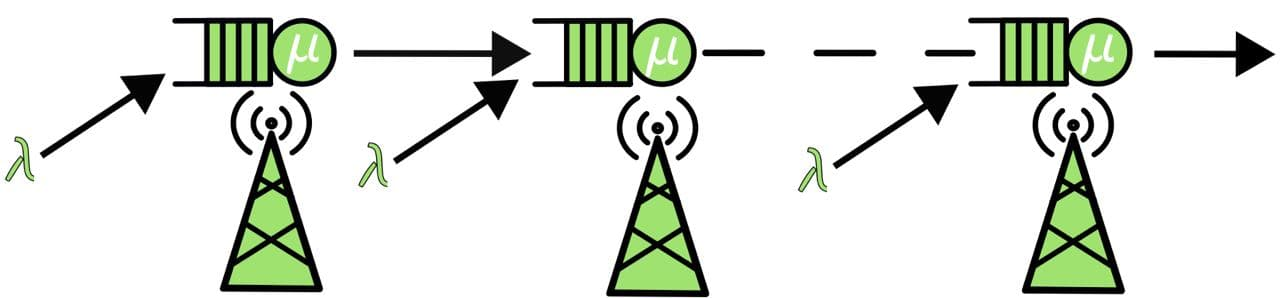
\includegraphics[width=1\textwidth]{tandem_queue.png}
\caption{СеМО с кросс-трафиком и узлами $M/M/1$.}
\label{fig:tandem_queue}
\end{figure}

На вход каждой станции поступает пуассоновский поток. Пуассоновский процесс представляет собой случайный процесс, характеризующийся  экспоненциально распределенным временем между событиями. Это один из наиболее важных случайных процессов в теории вероятностей, который широко используется для моделирования поведения трафика и входов во многих коммуникационных сетях и системах \cite{Kalor2018, Gao2016, Malandra2018, Seliem2019}. 

В пуассоновском процессе события происходят непрерывно и независимо друг от друга. Функция распределения имеет вид  \cite{VishnevskyBook, Kleinrock1975}:

\begin{displaymath}
P(X<x) = 
  \begin{cases}
    1 - e^{- \lambda x}, \quad x \geqslant 0; \\
    0, \quad x < 0.\\
  \end{cases}
\end{displaymath}

Для входящего потока, интервалы между поступлениями заданны случайной величиной c экспоненциальным распределением и интенсивностью $\lambda$. Время обслуживания на узле задана также экспоненциальным распределением и интенсивностью $\mu$. 


По теореме Бурке \cite{Burke1956}, поток на выходе узла $M/M/1$, а значит на входе каждой последующей фазы тоже пуассоновский. Интенсивность на выходе каждой фазы равна суммарной интенсивности всех входящих потоков с интенсивностями $\lambda$.

Пропускная способность на практике часто составляет половину от заданной в спецификации оборудования \cite{Proletarsky, Vladimirov2019}. Интенсивность времени обслуживания рассчитывается по формуле: 

\begin{displaymath}
    \mu_j = 0.5 \cdot p_j / w,
\end{displaymath}
где: $p_j$ - пропускная способность $j$-ой станции, Мбит/с; $w$ - средний размер пакета, Мбит.

Для каждой станции коэффициент загрузки равен:


\begin{displaymath}
\rho_j= \frac{\sum{\lambda}}{\mu_j} = \frac{q \cdot \lambda}{\mu_j} <1,
\end{displaymath}
где $q$ -- число входящих потоков. Условие $\rho_j<1$ является необходимым и достаточным условием существования стационарного режима функционирования СеМО.

Далее по формуле Литтла \cite{Little1961} можно рассчитать время задержки на каждой станции:

\begin{displaymath}
    \overline{T_j} = \frac{\rho_j}{1 - \rho_j} \cdot \frac{1}{q \cdot \lambda}.
\end{displaymath}

Тогда межконцевая задержки в сети равна

\begin{equation}
    \label{eq:end_to_end_delay}
    \overline{T}= \sum{\overline{T_j}}.
\end{equation}


Существуют более сложные модели очередей для оценок характеристик с более сложными распределения входящего трафика и времени обслуживания. Адекватные оценки дают модели с коррелированными входным потоком \cite{Vishnevsky2016_Methods_of_performance, Larionov2019}. К сожалению, такие модели труднорешаемы и для большего числа фаз СеМО не имеют аналитических расчетов. В данном исследовании будем использовать простейшую модель СеМО с узлами $M/M/1$ на этапе задачи оптимального размещения. Согласно предложенной концепции проектирования, полученную БШС с размещенными БС и выбранным техническим оборудованием можно будет в дальнейшем проводить на более сложных моделей на следующем этапе моделирования сети. Этот этап включает в себя математическое, имитационное моделирования для оценок характеристик производительности как время задержек, длины очередей, пропускная способность, вероятность потери пакетов и др. Данный этап позволяет провести комплексную проверку соответствия QoS для полученного размещения БС.

\section{Выводы по главе 1}

В главе представлено актуальность внедрения БШС в рамках цифровой трансформации нефтегазового сектора <<Индустрия 4.0>>. Представлены тематика исследования и задачи, затронутые в диссертации в рамках данного внедрения, а именно задачи синтеза топологии при проектировании беспроводных телекоммуникации на месторождении. Представлена структура последовательностей этапов при проектировании и место задачи синтеза в ней. Представлены методика расчета параметров БС необходимых в дальнейшем для оптимизационных задач размещения БС. 

% \begin{figure}[h!]
%   \centering
%    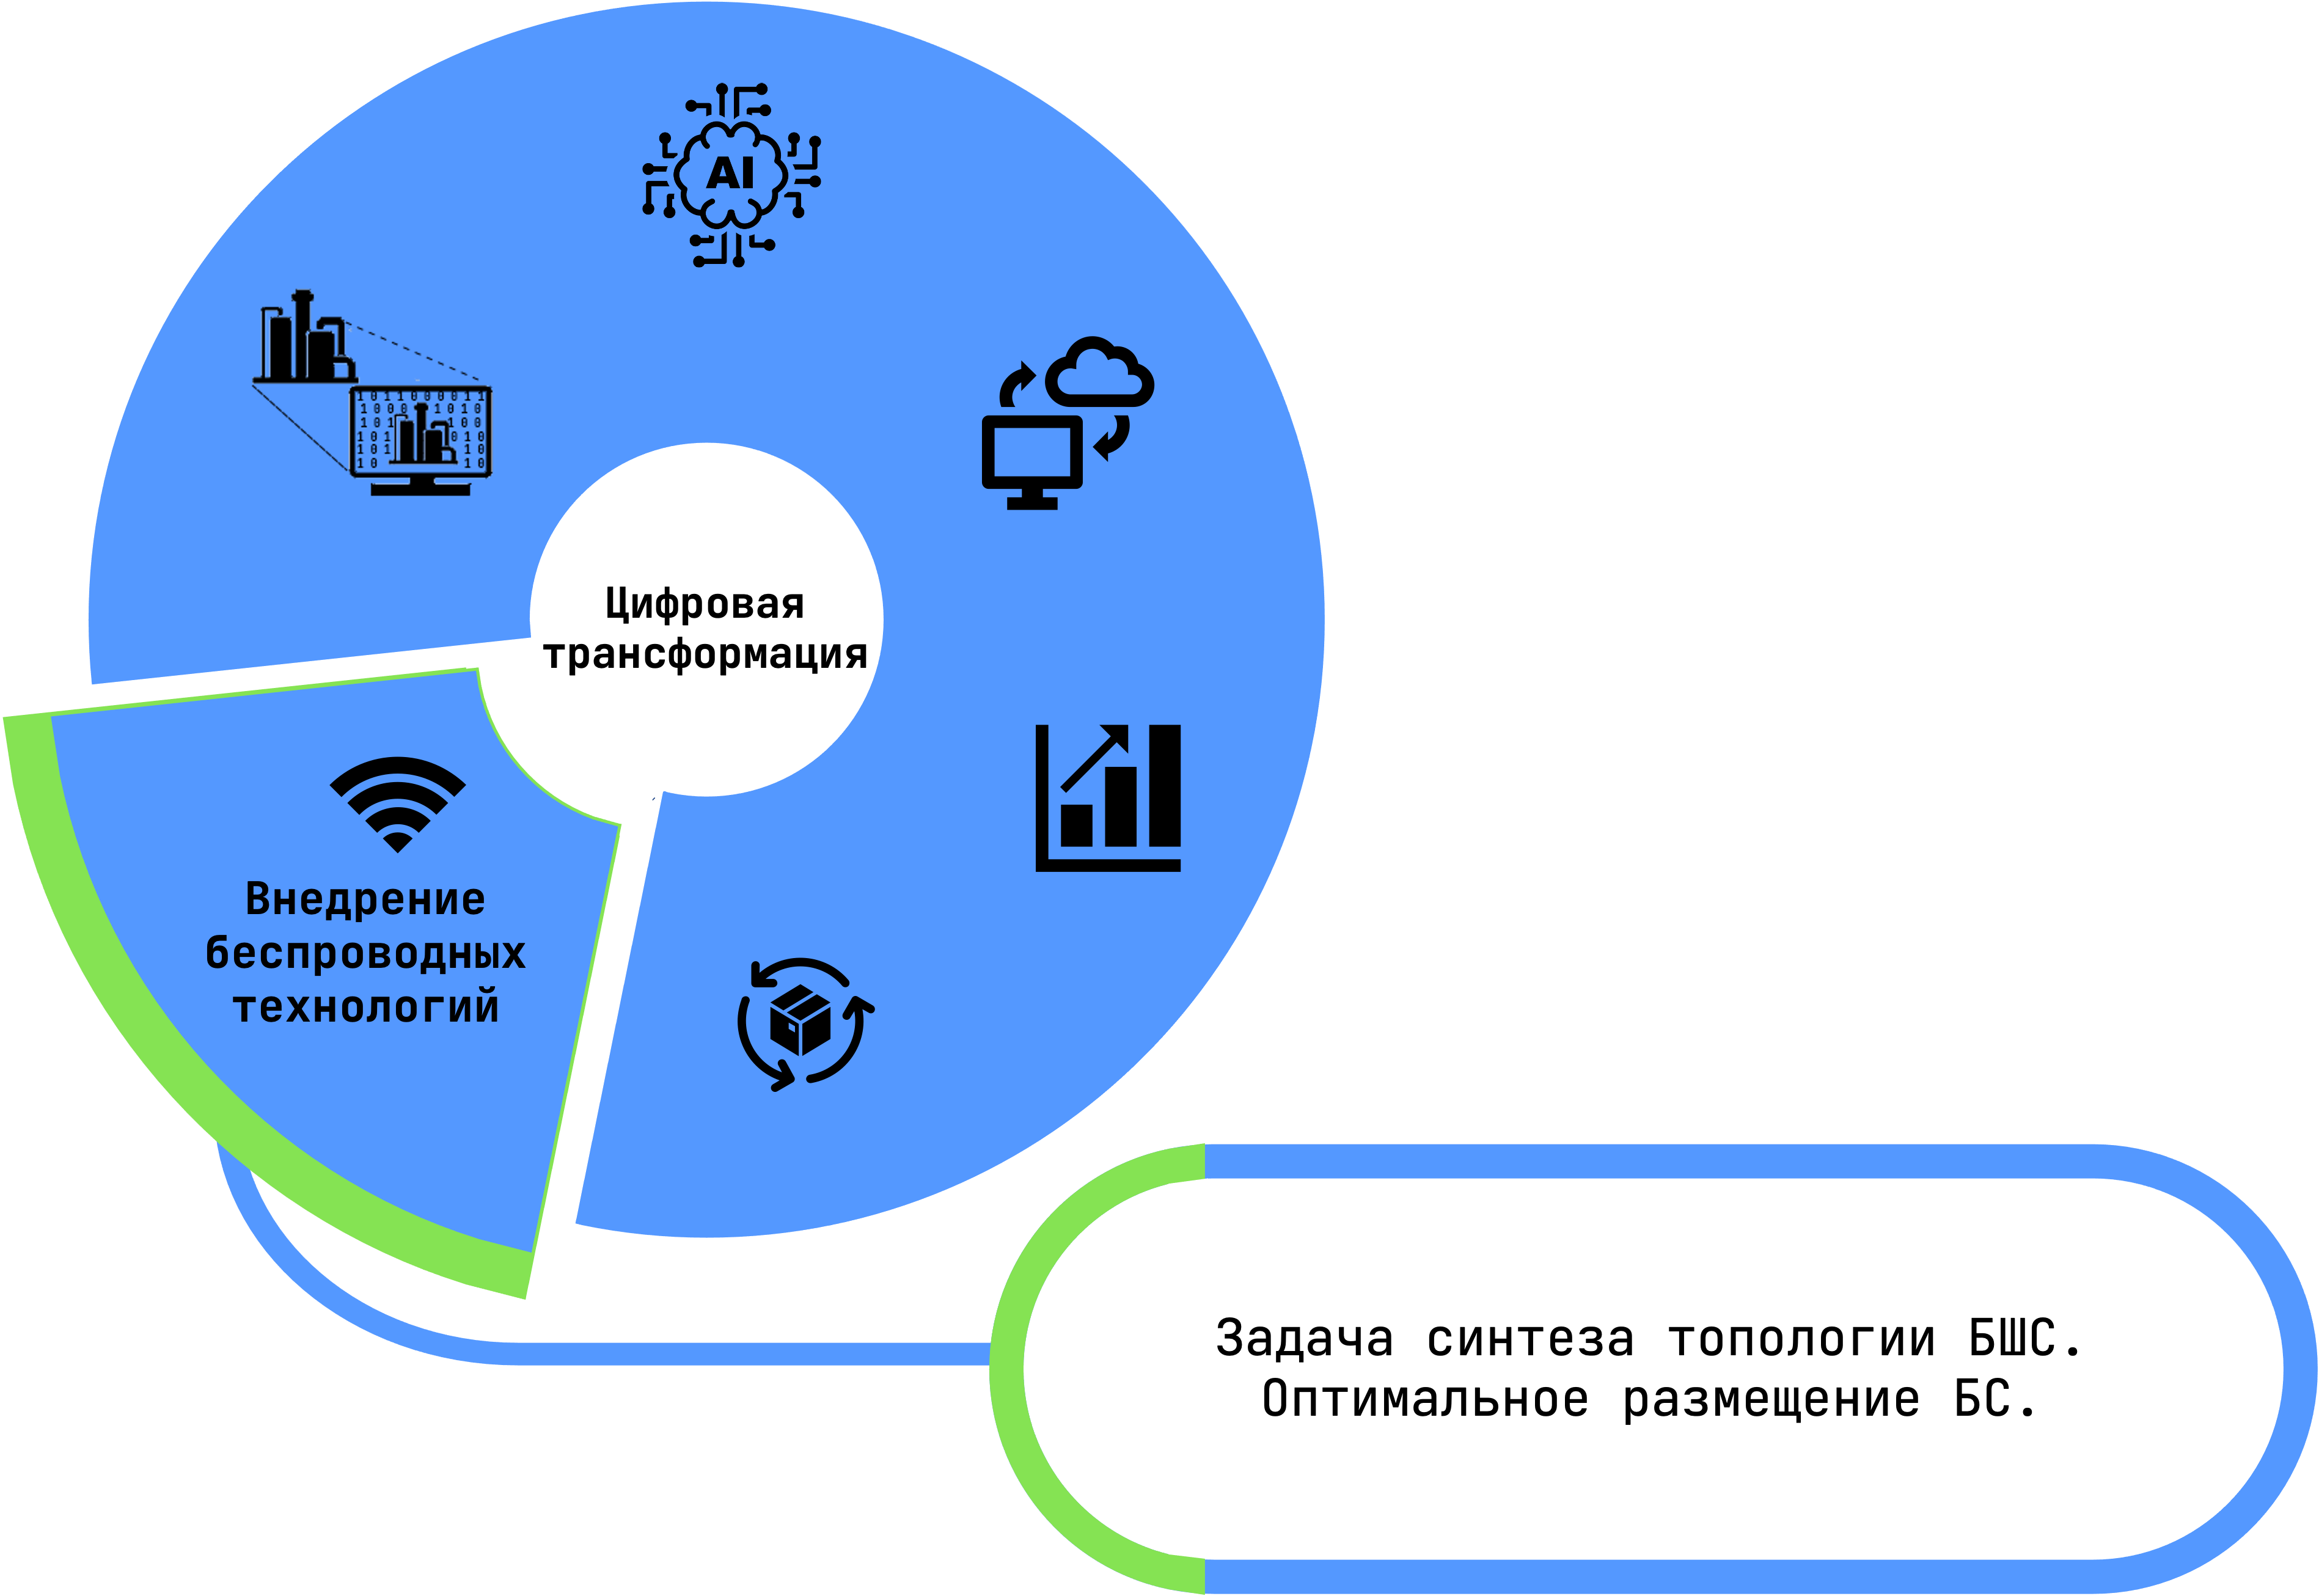
\includegraphics[width=1\textwidth]{industry4.png}
% \caption{Задача синтеза топологии при проектировании БШС в рамках цифровой трансформации "Индустрия 4.0".}
% \label{fig:industry4}
% \end{figure}





\FloatBarrier
           % Глава 1
\chapter{Задача оптимального размещения базовых станций БШС для контроля линейной территории}\label{chapter_linear_network}
% \chapter{Математические модели синтеза топологии сети для охвата линейного участка в виде задачи целлочисленного линейного программирования}\label{chapter_ilp_model}
\section{Актуальность внедрения БШС для линейном участке на месторождении}

В данной главе будет представлена математическая модель размещения БС БШС вдоль линейного участка. Ключевым таким линейным объектом на нефтегазовом промысле является магистральный трубопровод. 

Магистральные трубопроводы предназначены для транспортировки товарной нефти или газа из района промысла, производства до места потребления. В общем случае под местами потребления понимают нефтебазы, перевалочные базы, пункты налива в цистерны и заводы \cite{Deineko2018}. В зависимости от географических особенностей и климатических условий магистральные трубопроводы могут прокладываться в подземном, наземном или надземном типах.

Трубопроводы по-прежнему являются самым безопасным способом транспортировки нефти, но случайных утечек избежать невозможно.  К особо уязвимым участкам трубопроводной инфраструктуры относятся регулирующая арматура, ловушки для скребков, приемники скребков, счетчики и манометры.
Хотя утечки в трубопроводе часто начинаются с малого, позднее обнаружение и идентификация утечек может иметь пагубные последствия. Для нефтегазовой компании несвоевременное обнаружение может нанести миллионы финансовых убытков, а также нанести ущерб репутации и окружающей среде.

Основными причинами аварийных ситуаций на линейных участках являются: коррозионные разрушения, механические повреждения при строительстве и эксплуатации, а также заводские браки \cite{Deineko2018_alone}. Отсюда возникает важная задача, с которой сталкиваются компании на промысле -- отслеживание состояния трубопроводов, по которому транспортируются нефть и газ \cite{Aalsalem2018}. Эффективным средством прогнозирования и предотвращения отказов и аварийных ситуаций на магистральных трубопроводах, а также экологической защиты и достижения промышленной безопасности становится мониторинг нефтепровода, путем внедрения беспроводных сетей связи, включающее беспроводных техничеких средств для диагностики технического состояния трубопроводов, измененений под влиянием геологических процессов на опасных участках \cite{Krzyszton2021,Mehmood2016, Lin2019, Adegboye2019}; а также внедрения беспроводных систем видеонаблюдения, в том числе БПЛА позволяющий контролировать безопасность на всем участке трубопровода \cite{Fedorova2020, Aljuaid2020, Adegboye2019, Gomez2017, Fawzi2019}.


Одним из интересных направлений является организация беспроводных сетей для обнаружения утечек и отслеживания границ и направления движения токсичных газов с помощью мобильных беспроводных сенсорных устройств \cite{Krzyszton2021}. В работе \cite{Lin2019} предлагается беспроводная сенсорная сеть для мониторинга утечек вдоль подземных трубопроводов.С учетом уже широкого применения беспроводных сенсорных сетей в нефтегазовой отрасли, все еще существуют некоторые
проблемы при их развертывании: вероятность потерь передачи сигнала между сенсорами, отказы узлов и проблемы с энергопотреблением, особенно для линейной топологии \cite{Lee2020}. Беспроводные сенсорные сети, уже широко применяются на месторождениях. К сожалению, большинство используемых методов маршрутизации не предназначены для линейной топологии \cite{Abbas2018}. В простейшем случае, когда отказывает один узел, вся сеть перестает функционировать. Беспроводные сенсорные сети на базе протоколов WirelessHart, IEEE 802.15.4, ISA100.11a и др. нашли свое широкое применение в нефтегазовом секторе. В силу ограничения дальности связи данных протоколов целесообразно объединять такие сенсорные сети вдоль линейного сооружения в БШС дального радиуса действия на базе семейства протоколов IEEE 802.11 (Рис. \ref{fig:part2_pipeline}). Для сбора данных с сенсорной сети вдоль линейного объекта используются узлы транспортировки сети -  базовые станции \cite{Fataliyev2018}.  Использование базовых станций в сенсорных сетях позволяет увеличить связность сети, путем разбиение сети на мелкие кластеры. Повышение связности сети при ее разбиении достигается вследствие того, что базовая станция является более надежным узлом, имеет большую дальность уверенной передачи радиосигнала, меньше зависит от ограничений в энергопотреблении \cite{Krasnov2016}.

\begin{figure}[ht]
  \centerfloat{
      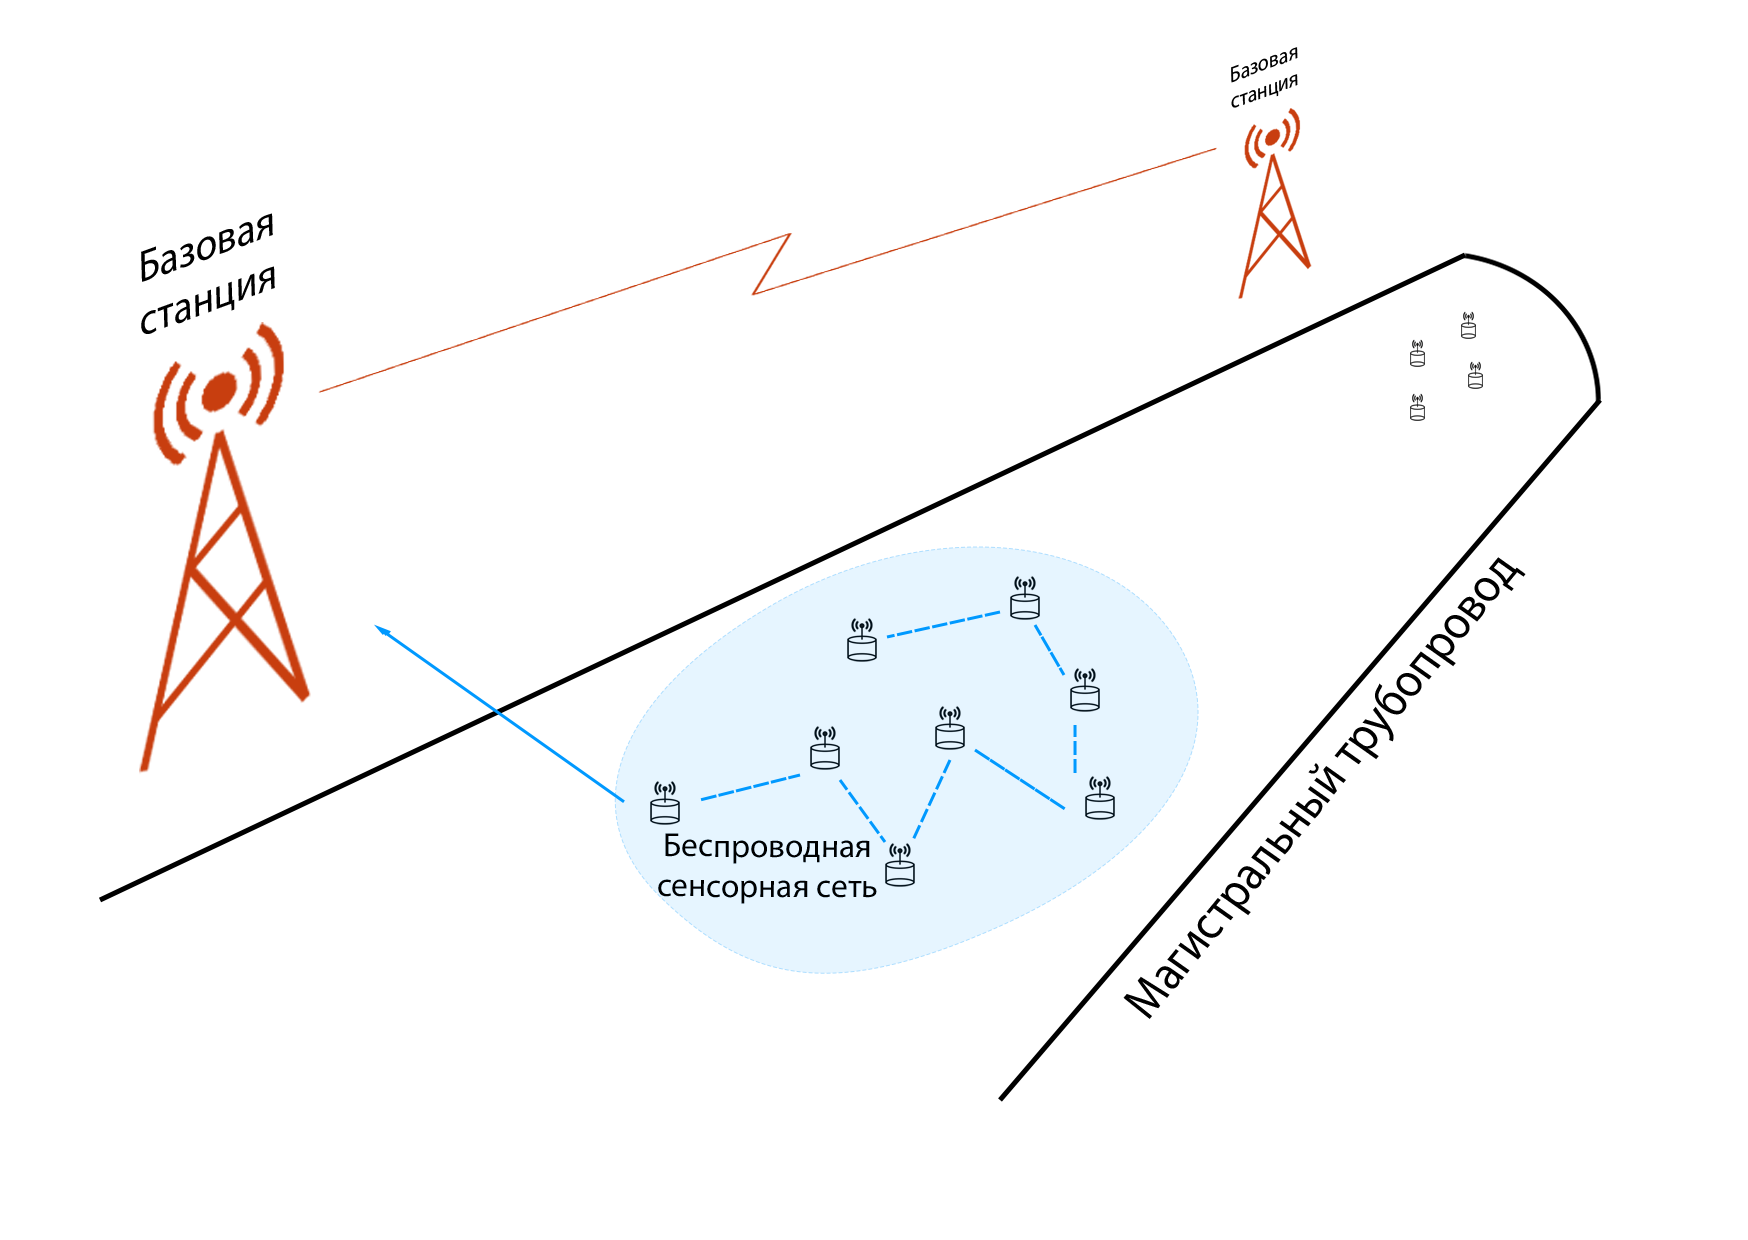
\includegraphics[scale=1.1]{pipeline.png}
  }
  \caption{Беспроводная сеть вдоль магистрального трубопровода}\label{fig:part2_pipeline}
\end{figure}

В \cite{Anupama2014, Jawhar2007} авторы предлагают иерархическую сенсорную сеть для мониторинга трубопроводов, в которой третим уровенем иерархии сети являются базовый станции, покрывающие весь линейный участок.

Один из современных методов обнаружение утечек и мониторинга в реальном времени является использование беспроводной сети связи на базе стационарных объектов -- базовых станций и  беспилотных летательных аппаратов  (БПЛА, Unmanned Aerial Vehicle, UAV) \cite{Aljuaid2020}. В \cite{Fedorova2020} рассматривается использование БПЛА для мониторинга нефтепроводов. Предлагается математическая модель для определения состава группы БПЛА и метода ее базирования.

Еще одним немаловажным линейным объектом любого промысла, требующим постоянного контроля является сеть промысловых дорог. С учетом большой удаленности друг от друга объектов нефтегазовой отрасли друг от друга целесооборазно организовать телекоммуникациионную сеть вдоль протяженных автодорог для контроля данного линейного участка с помощью информации с систем видеонаблюдения \cite{Vish2015} (Рисунок \ref{fig:part2_roadisdeunit}). Одним из наиболее перспективных решений на транспорнтных участках является организация автомобильных сетей (Vehicular ad hoc network, VANET) \cite{Massobrio2020, Campolo2015}. Для решение данной проблемы хорошо подходит БШС. Организации БШС вдоль автодорог посвящено ряд зарубежных и отчествевенныз работ. 

\begin{figure}[ht]
  \centerfloat{
      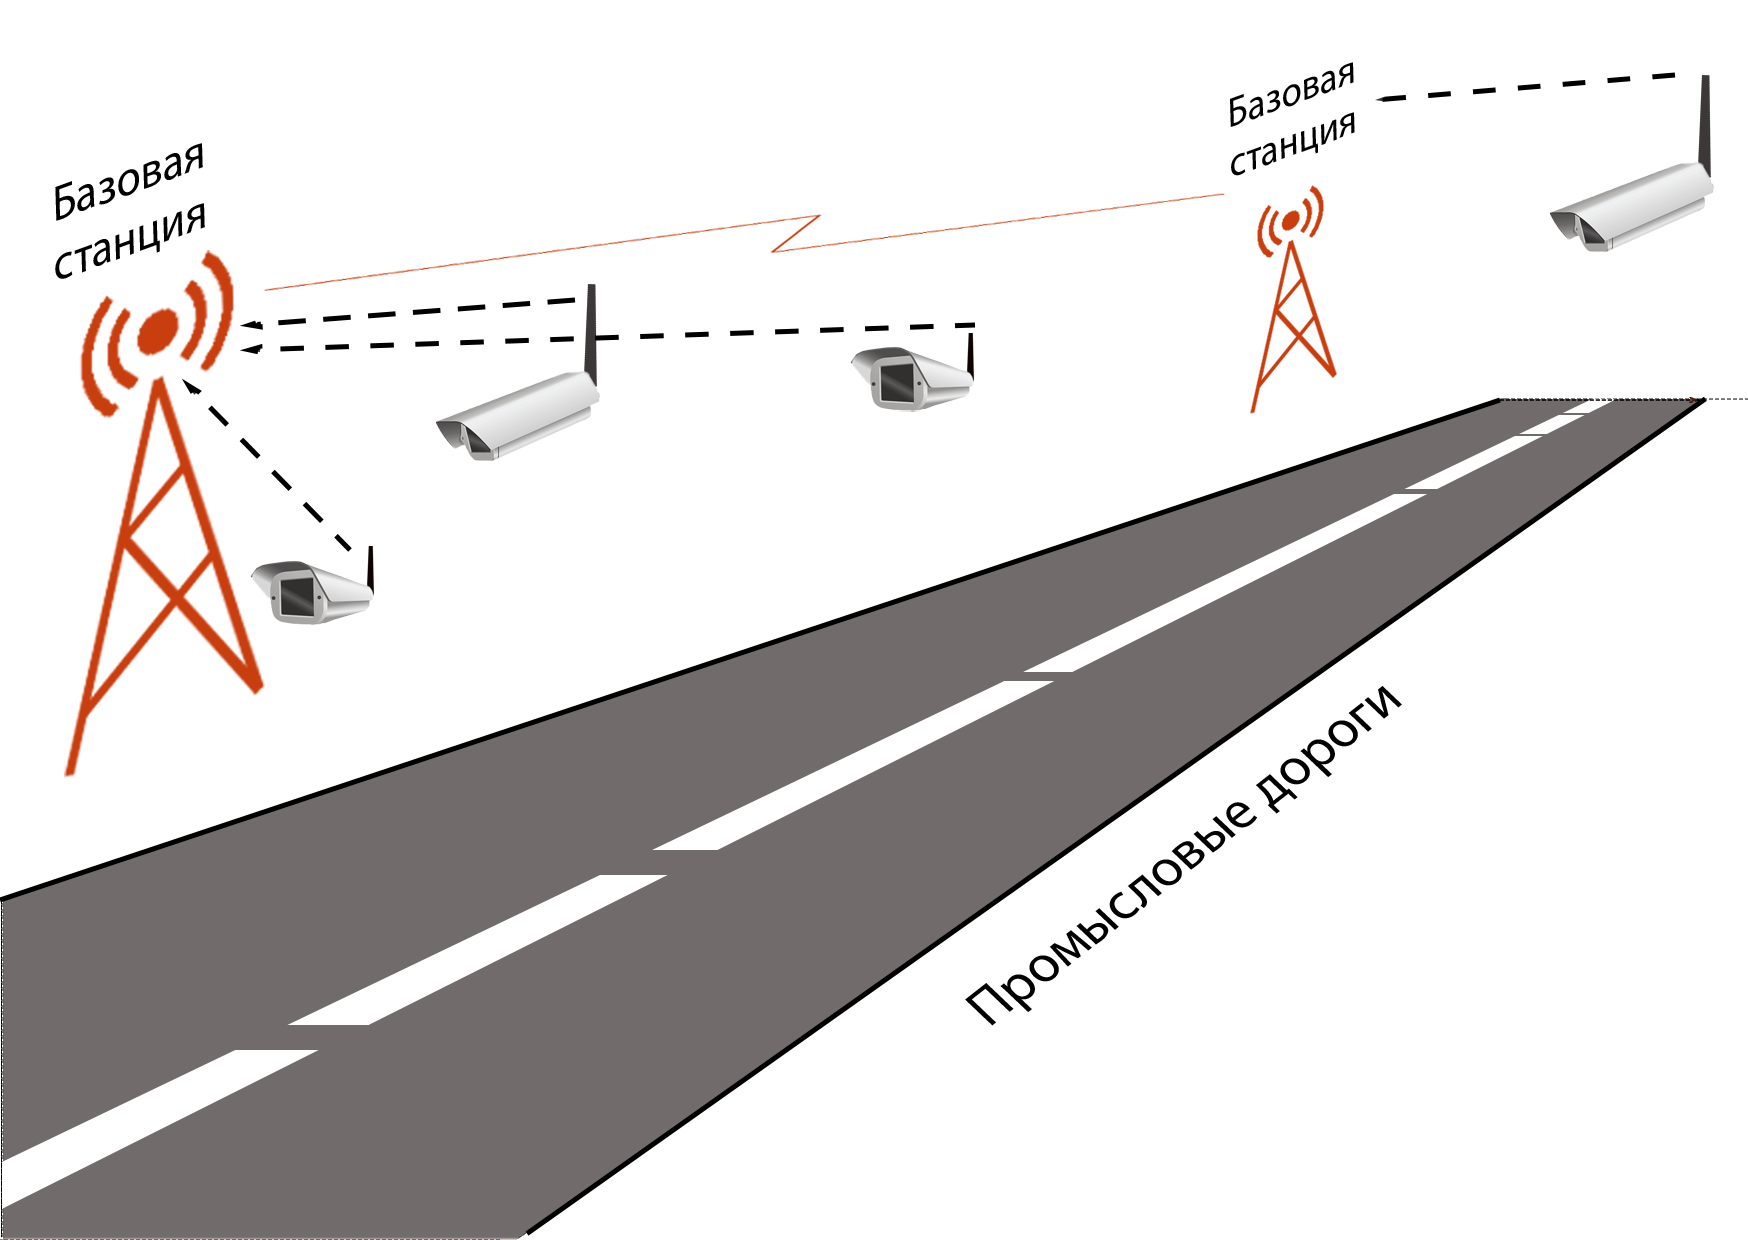
\includegraphics[scale=1.1]{roadsideunit.png}
  }
  \caption{Беспроводная сеть вдоль промысловых дорог}\label{fig:part2_roadisdeunit}
\end{figure}





\section{Математические модели синтеза топологии сети для охвата линейного участка в виде задачи целлочисленного линейного программирования}
% \section{Introduction}
% Wireless technologies are widely used in various areas of human life. Wireless broadband communication networks are used for operational control of industrial or civil objects, technological plants, smart moving vehicles. The use of wireless broadband technologies based on the IEEE 802.11 protocols family to organize such networks has several advantages over wired technologies. These include rapid deployment of communication networks, convenient modernization and scalability of the network architecture, and reduced installation and maintenance costs.

% To improve the design efficiency of such a modern information transmission infrastructure, it is crucial to solving the problem of optimal placement of equipment, in our case, base stations of a wireless broadband communication network at various possible locations. A similar problem has been proposed and discussed in several works \cite{KHireddine2020,BenBrahim2014,Chattopadhyay2018,KIZILOZ2020,Liu2014,Reis2014,Shen2020}.

% This work is a continuation of the researches \cite{Ivanov2018} and \cite{Ivanov2019}, where the particular case of the problem is considered when the controlled area is a linear section, for example, the area along highways, the linear part of trunk pipelines, field communications. In the above papers, the formulation was given in the form of an integer linear programming model. The proof of NP -- completeness was presented.

% The problem considered in the previous work \cite{Ivanov2019} it was necessary to place a given base station set formed at the previous network design stages. The present paper considers a more general case when solving an optimization problem is also determined by a set of placed stations from a given redundant set while respecting technical and economic constraints. This paper presents the preparation of main station characteristics, such as the coverage radius, link distance, and station service time. We need to prepare these characteristics before proceeding to the optimal placement problem.  The paper proposes the problem in the form of an integer linear programming with the input of the above-calculated characteristics into the problem conditions with the end-to-end delay constraint. This restriction significantly impacts the mathematical model form of the problem.





Размещение БС вдоль линейного участка приобретают все большую актуальность на сегодняшний день. Большиство работ касаются проблемы размещения придорожных объектов (Roadside Unit, RSU) или другими словами БС вдоль автодорог. 

Задача оптимального размещения БС нашла свое широкое отражениие в исследованиях зарубежных и отечетсвенных авторов. Большиство работ касаются проблемы размещения придорожных объектов (Roadside Unit, RSU) или другими словами БС вдоль автодорог. В \cite{Cavalcante2012} предложена модель, используюящая генетический алгоритм для решения задачи о максимальном покрытии. Максимизация покрытия БШС с учетом ограничения стоимости БС представлена в работах \cite{BenBrahim2014, Vishnevsky2016_optimization}. В работах \cite{Liu2014, Gao2018, Jalooli2019} предложены новый модели размещения БС с учетом характеристик трафика на участках. В \cite{Reis2014} представлена задача размещения БС для протокола IEEE 802.11p/Wave. В \cite{Guerna2021} предложена модель размещения БС с помощью муравьиного алгоритма. В работах \cite{Cavalcante2012, Liu2017} в качестве ограничений учитываются временные ограничения при размещения БС. В \cite{Bao2018} предлагают жадный алгоритм для минимизации RSU c условием ограничения задержек между любыми двумя узлами сети. В работе \cite{Ivanov2018} представлена задача размещения RSU вдоль линейного участка протяженной автомагистрали. 


Представление задачи размещения БС вдоль автодорог в виде одномерной задачи нашло свое широкое применение \cite{Ivanov2018, Reis2014, Vishnevsky2016_optimization, Liu2014, Gao2018, Jalooli2019, Zhang2017}. В нашем случае является также эффективным для применения вдоль промысловых дорог между удалленными на большие расстояния объектами нефтегазовых отрасли.

Задача размещения также актуально для беспроводных сетей. В работе \cite{Alduraibi2016} предложены модели размещения узлов беспроводной сенсорной сети (WSN, Wirelss Sensor Network), максимизирующий покрытие линейного участка трубопровода. В \cite{Aria2020} авторы представляют во внимание модель размещения узлов WSN обнаружения повреждений на трубопроводе, учитывающие зоны, которые будет контролировать только обслуживания персонал. В работах \cite{Hussein2020, Varshney2018, Varshney2021} представлены модели размещения узлов WSN минимизирующее суммарное энергопотребление. В \cite{Li2020, Albaseer2019} предложен модели кластеризации узлов БШС, в \cite{Albaseer2019} предлагают модели БШС для мониторинга утечек вдоль нефте-- и газопроводов.

\subsection{Постановка задачи}

В отличии от большинства реализаций БШС вдоль трубопроводов, где используется одноуровневая реализация сети, в данной диссертации, согласно широко используемой классификации \cite{Jawhar2009, Varshney2015, Abbas2018, Wang2011, Jawhar2013}, будет предложено иерархическая БШС сеть c линейной топологии. Данные с полевых измерительных устройств собираются шлюзом. Именно с этих шлюзов вся информация будет собираться через систему размещенных БС. В случае проектирования БШС для видеонаблюдения, вся поток будет идти на БС непосредственно с антенн камер видеонаблюдения.


Проблема формулируется следующим образом. Для контроля над заданным линейным участком необходимо разместить базовые приемопередающие станции (далее называемые станциями) таким образом, чтобы максимизировать покрытие с ограничением на суммарную стоимость размещенных станций. Важно обеспечить связи любой станции со шлюзами на концах участка через систему размещенных станций.

Задано множество станций $S = \{s_j\}$. Каждой станции приписаны параметры $s_j = \{r_j, \{R_{jq}\}, c_j \}$, $j = \overline{1,m}; q = \overline{1,m}; q \neq j$. Здесь $r_j$ -- радиус покрытия станции, $R_{jq}$ -- это радиус связи между станцями $s_j$ и $s_q$, и $c_j$ -- это стоимость. 

Задан линейный участок длиной $L$ с концами в точка $a_0$ и $a_{n+1}$. Внутри  отрезка $[a_0, a_{n+1}]$ задано конечное множество точек $A=\{a_i\}, i=\overline{1,n}$; эти точки соответствуют набору свободных мест, где могут быть размещены станции. Каждая точка $a_i$ определяется своей одномерной координатой $l_i$.

Заданы станции специального вида $s_{m+1}$ -- шлюзы. Данные шлюзы размещены на концах $a_0$ и $a_{n+1}$ данного линейного участка . Для данных станций параметр радиуса покрытия $r_{m+1}=0$. Радиус связи и стоимость не заданы.

Требуется разместить станции таким образом, чтобы максимизировать покрытие с условием ограничения на суммарное стоиомсть $C$.

 

% \section{Расчет дальности действия связи}


% Перед тем как приступить к задаче ЦЛП необходимо рассчитать характеристики станции: радиус связи $R_{jq}$ и радиус покрытия $r_j$.

% При развертывания сети необходимо обеспечить максимальное покрытие данного участка связь между шлюзами через систему размещенных базовых станций беспроводной широкополосной сети.

% Для оценки производительности канала связи воспользуемся уравнением энергетического потенциала. Полное уравнение можно записать следующим образом:

% % It is essential during deployment to provide maximum coverage of a given area and ensure communication between the placed base stations in the wireless broadband network. 

% % Link Budget is a way of estimation of communication link's performance while accounting for the system's power, gains, and losses for both the transmitter and receiver. The complete equation can be written as follows:

% \begin{equation}
%   \label{eq:part3_link_budget}
%   P_{tr} - L_{tr} + G_{tr} - L_{fs} + G_{recv} - L_{recv} = SOM + P_{recv},
% \end{equation}
% где:

% \begin{itemize}

%   \item $P_{tr}$ -- мощность передатчика, дБм;

%   \item $L_{tr}$ -- потери сигнала на антенном кабеле и разъемах передающего тракта, дБ;

%   \item $G_{tr}$ -- усиление антенны передатчика, дБ;

%   \item $L_{fs}$ -- потери в свободном пространстве, дБ;

%   \item $G_{recv}$ -- усиление антенны приемника, дБ;

%   \item $L_{recv}$ -- потери сигнала на антенном кабеле и разъемах приемного тракта, дБ;

%   \item $SOM$ -- запас на замирание сигнала, дБ;

%   \item $P_{recv}$ -- чувствительность приемника, дБм.

% \end{itemize}

% Мощность принимаемой антенны рассчитывается из уравнения передачи Фрииса:

% \begin{displaymath}
%   \label{eq:part3_Friis}
%   \frac{P_{recv}}{P_{tr}} = G_{tr}G_{recv}\left(\frac{c}{4\pi R f} \right)^2,
% \end{displaymath}
% где
% $c$ --  скорость света,
% $f$ -- частота, 
% $R$ рассточние между приемной и передающей антенной.

% The Free Space Path Loss ($ FSPL $) equation defines the propagation signal loss between two antennas through free space (air):

% Уравнение потерь в свободном пространстве (Free Space Path Loss, $FSPL $) определяет потерю сигнала при распространении между двумя антеннами в свободном пространстве (в воздухе):

% \begin{equation}
%   \label{eq:part3_FSPL}
%   FSPL = \left(\frac{4\pi R f}{c} \right)^2.
% \end{equation}

% Формула (\cref{eq:part3_FSPL}), выраженная в децибеллах будет выражаться как

% \begin{equation}
%   \label{eq:part3_L_fs}
%   L_{fs} = 20 \lg{F} + 20\lg{R} + K,
%   \end{equation}
% где $F$ -- центральная частота, на котором работает канал связи, $R$ -- рассточние между приемной и передающей антенной и $K$ -- константа.

% Константа $K$ зависит от размерностей частоты и расстояния:

% \begin{itemize}
%   \item для чистоты, выраженной в ГГц, и рассчтояния, выраженная в км, константа $K$ равна 92.45;
%   \item для чистоты, выраженной в МГц, и рассчтояния, выраженная в км, константа $K$ равна 32.4;
%   \item для чистоты, выраженной в МГц, и рассчтояния, выраженная в м, константа $K$ равна -27.55.
% \end{itemize} 

% Потерия $L_{fs}$ выразим из формулы (\cref{eq:part3_link_budget}) как:

% \begin{equation}
%   \label{eq:part3_L_fs_from_link_budget}
%   L_{fs} = P_{tr} - L_{tr} + G_{tr} + G_{recv} - L_{recv} - SOM - P_{recv}.
% \end{equation}

% Радиус связи получаем из уравнений (\cref{eq:part3_L_fs}) и (\cref{eq:part3_L_fs_from_link_budget}):

% \begin{equation}
%   \label{eq:part3_D}
%   R = 10^{\left(\frac{L_{fs} - 20\lg{F} - K}{20}\right)}.
% \end{equation}

% Используя формулу \cref{eq:part3_D} и \cref{eq:part3_L_fs_from_link_budget}, мы можем расчитать теоритическое максимальную дальность связи $ R_{jq}$ между базовыми станциями и радиусом покрытия $ r_j $ с предположением об отсутствии препятствий, отражений, влияния контуров местности и т. д. Это допущение приемлемо для нашего случая с открытой местностью.

% \begin{figure}[h!]
%   \centering
%    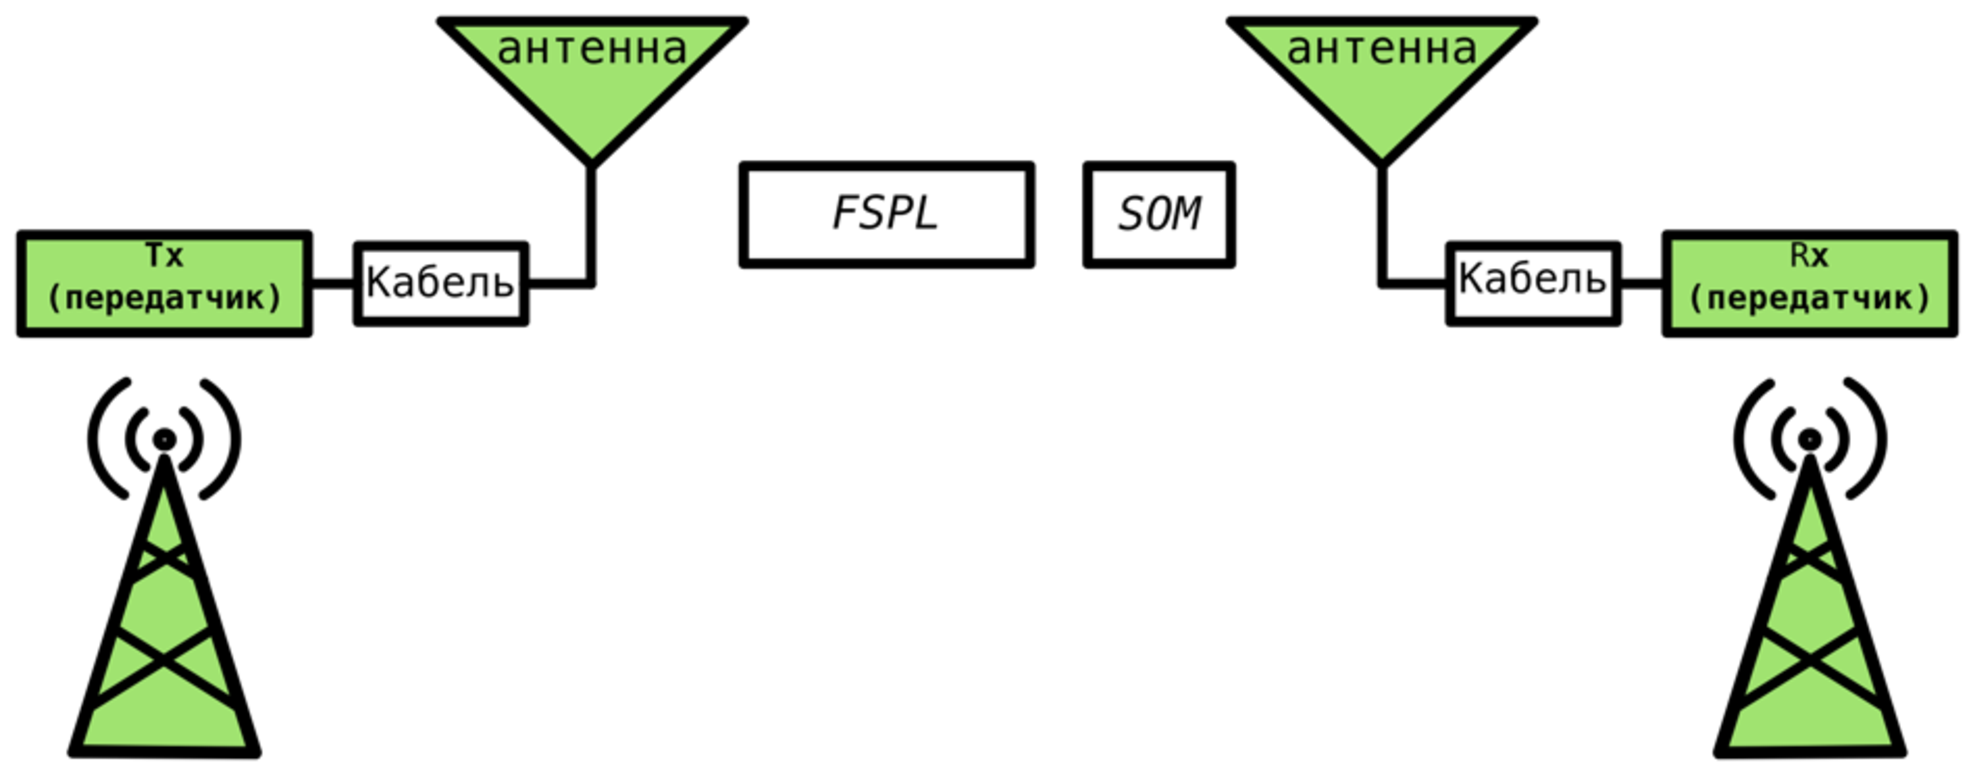
\includegraphics[width=0.8\textwidth]{link_distance.pdf}
% \caption{Соеденинение между станциями.}
% \label{fig:part3_link_distance}
% \end{figure}

% Для расчета дальности связи $R_{jq}$ (Рис. \cref{fig:part3_link_distance}), базовые станции $s_j$ и $s_q$ будут рассматриваться как станции \textit{передатчик} и \textit{приемник}, соответственно. Будем считать, что станции обрудованы направленными антеннами с усилениями $G_{tr}^{R}$ и $G_{recv}^{R}$.

% \begin{figure}[h!]
%   \centering
%    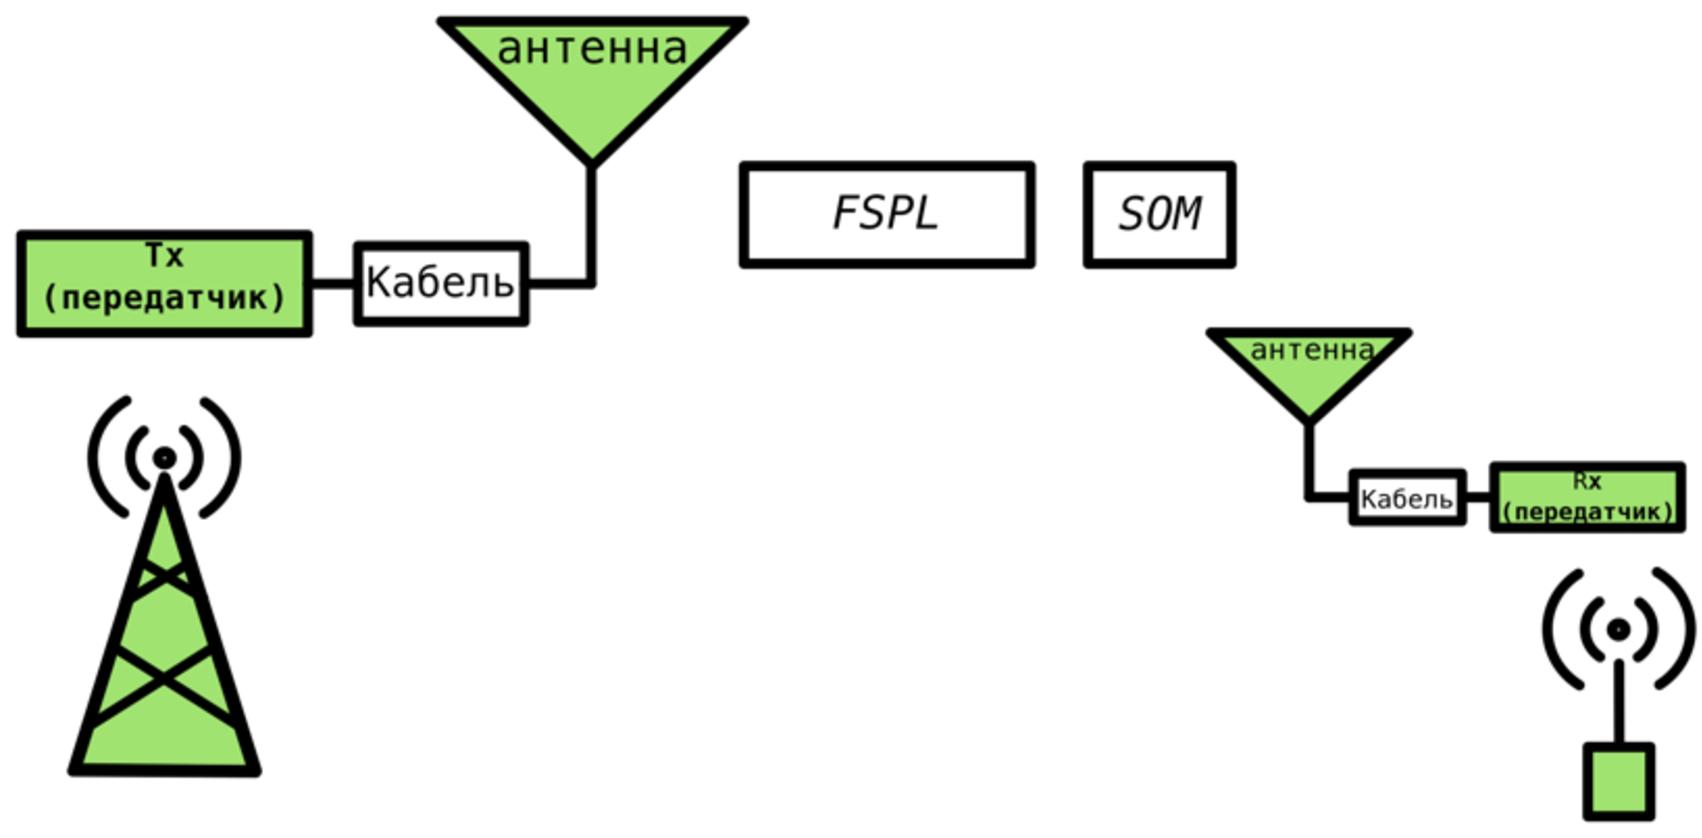
\includegraphics[width=0.8\textwidth]{coverage.pdf}
% \caption{Покрытие станции}
% \label{fig:part3_coverage}
% \end{figure}

% Каждая базовая станция оснащена всенаправленной антенной с заданным усилением антенны $G_ {tr}^{r}$. Данная антенн необходимо для покрытия заданной области.

% Each base station is equipped with an omnidirectional antenna with given gain antenna $G_{tr}^{r}$. A station uses this antenna to cover a given area.

% При вычислении радиуса покрытия $r_j$ (Рис.  \cref{fig:part3_coverage}) базовая станция будем считать \textit{передатчиком} а пользовательское устройство \textit{приемником}.

\subsection{Модель ЦЛП}

После оценки максимальных радиуса связи между станциями $R_{jq}$, максимального радиуса покрытия $r_j$, можно перейти, непосредственно, к задаче размещения станций в виде модели целочисленного линейного программирования.

Пусть $y_i^+$ и $y_i^-$ , $i= \overline{0,n+1}$ определяют охват покрытия (справа и слева, соответственно) станций, покрывающих точку $a_i$ (Рис. \cref{fig:part3_station_coverage}). Параметры $y_i^+$ и $y_i^-$ могут принимать только неотрицательные целые значения.

Величины  покрытия для шлюзов $y_0^+, y_0^-, y_{n+1}^+, y_{n+1}^-$ равны 0.

\begin{figure}[ht]
  \centerfloat{
      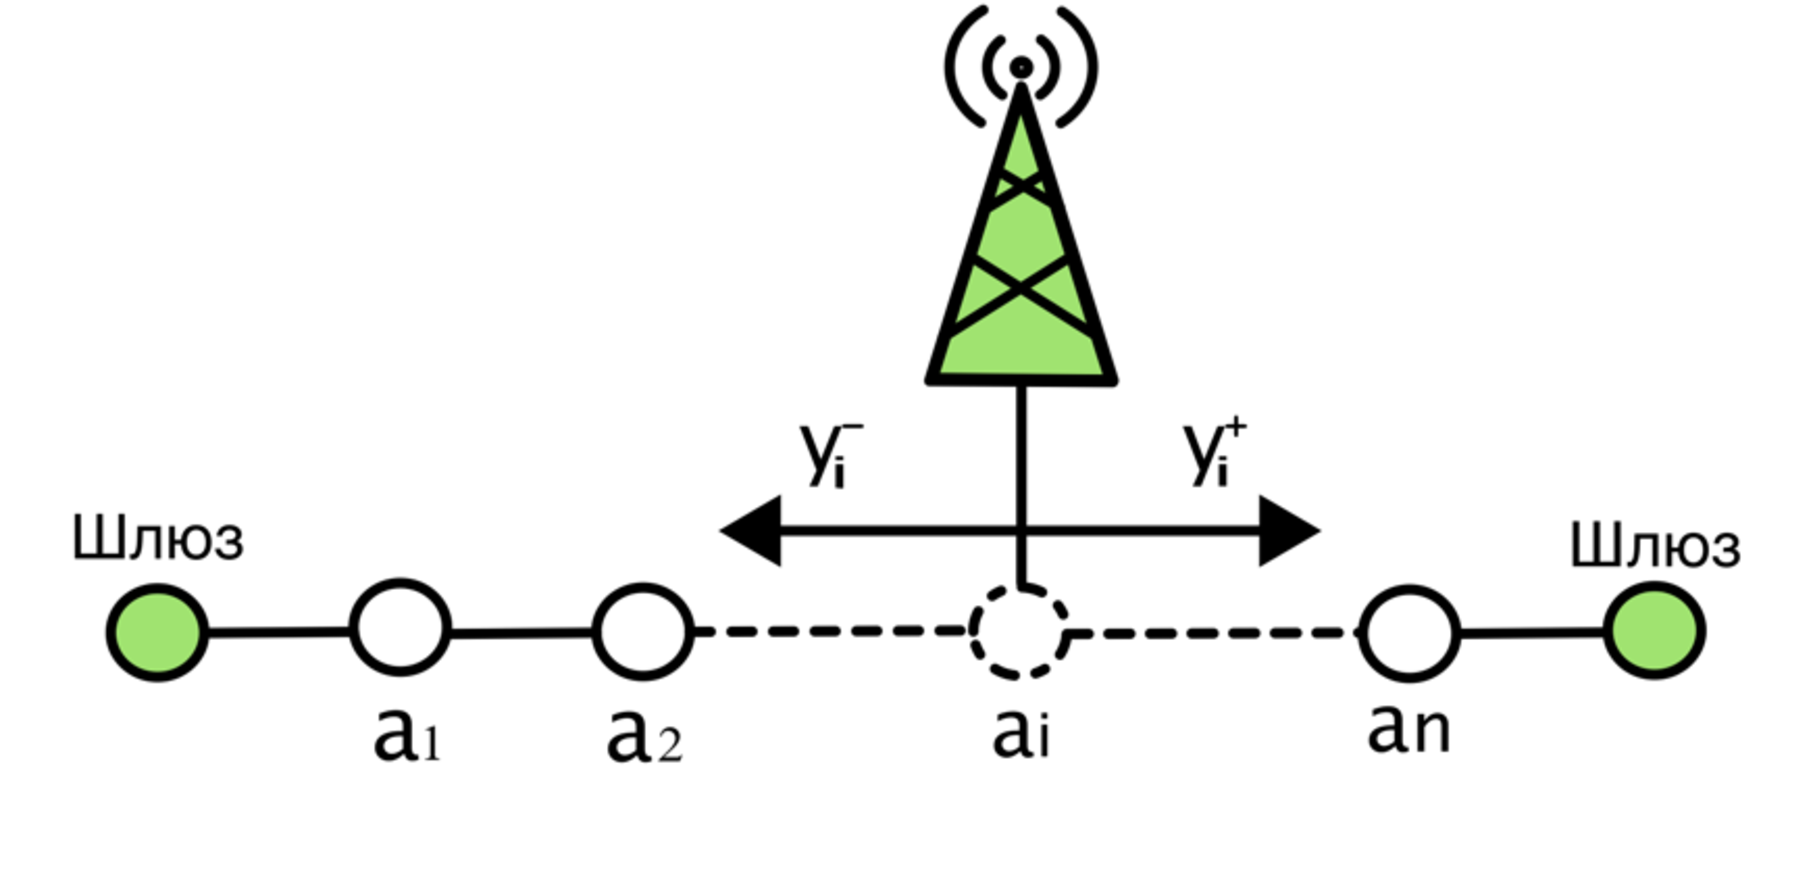
\includegraphics[scale=0.5]{station_coverage.pdf}
  }
  \caption{Охват покрытия станции}\label{fig:part3_station_coverage}
\end{figure}
 
Целевая функция будет представлена как:
\begin{equation}
  \label{eq:part3_objective_function}
  f =  \sum\limits_{i=1}^n (y_i^- + y_i^+) \rightarrow max
\end{equation}

Также введем бинарные переменные $x_{ij}$. Тогда $x_{ij}=1$, если станция $s_j$, размещенная на точке $a_i$, и $x_{ij}=0$ в противном случае; $i= \overline{1, n}$; $j = \overline{1,m}$.

Введем двоичные переменные $ e_i $. Тогда $ e_i = 1 $, если какая-либо станция находится в точке $ a_i $, и $ e_i = 0$  в противном случае; $ i = \overline {1, n} $. Для точек размещения шлюзов $ a_0 $ и $a_{n + 1}$ переменные $ e_0 = 1 $ и $ e_{n + 1} =1 $, соответственно. 

% Let us introduce binary variables $e_i$. Then $e_i$  is equal to 1, if any station is placed at point $a_i$ and $e_i$ is equal to 0 otherwise; $i = \overline{1, n}$. For gateways placement points $e_0$  is equal to 1 and $e_{n+1}$  is equal to 1.

Сформулируем следующую систему ограничений задачи.

По определению \cref{eq:part3_ei}:

\begin{equation}
  \label{eq:part3_ei}
  e_i =  \sum\limits_{j=1}^m x_{ij}, \quad i = \overline{1,n}. 
\end{equation}

Каждая станция должна быть размещена только в одной точке. \cref{eq:part3_xij}:

\begin{equation}
  \label{eq:part3_xij}
  \sum\limits_{i=1}^n x_{ij} \leq 1, \quad j = \overline{1,m}. 
\end{equation}

Значения покрытий не превышают радиус покрытия станции, размещенной в точке $ a_i $, и равны 0, если в точке $a_i$  нет станции \cref{eq:part3_yi_1, eq:part3_yi_2}:


\begin{equation}
  \label{eq:part3_yi_1}
  y_i^+ \leq \sum\limits_{j=1}^m x_{ij} \cdot r_j, \quad i = \overline{1,n};
\end{equation}

\begin{equation}
  \label{eq:part3_yi_2}
  y_i^- \leq \sum\limits_{j=1}^m x_{ij} \cdot r_j, \quad i = \overline{1,n}. 
\end{equation}

Общая область покрытия между любыми двумя точками $ a_i $ и $ a_k $, где расположены станции, не может превышать расстояние между этими точками \cref{eq:part3_yi_3, eq:part3_yi_4}.

\begin{equation}
  \label{eq:part3_yi_3}
  y_i^+ + y_k^- \leq \frac{l_k - l_i}{2} \cdot (e_i + e_k ) + (2 - e_i - e_k ) \cdot L, \quad i = \overline{1,n},  \quad k = \overline{i+1,n+1};
\end{equation}

\begin{equation}
  \label{eq:part3_yi_4}
  y_i^- + y_k^+  \leq \frac{l_i-l_k}{2} \cdot (e_i + e_k) + (2 - e_i - e_k) \cdot L, \quad i = \overline{1,n}, \quad k = \overline{i-1,0},
\end{equation}
где $ l_k $ и $ l_i $ - координаты точек $ a_i $ и $ a_k $, соответственно. Это условие исключает влияние пересечений покрытий станций при вычислении общего значения покрытия между станциями (Рис. \cref{fig:part3_total_coverage_between_points}).

\begin{figure}[ht]
  \centerfloat{
      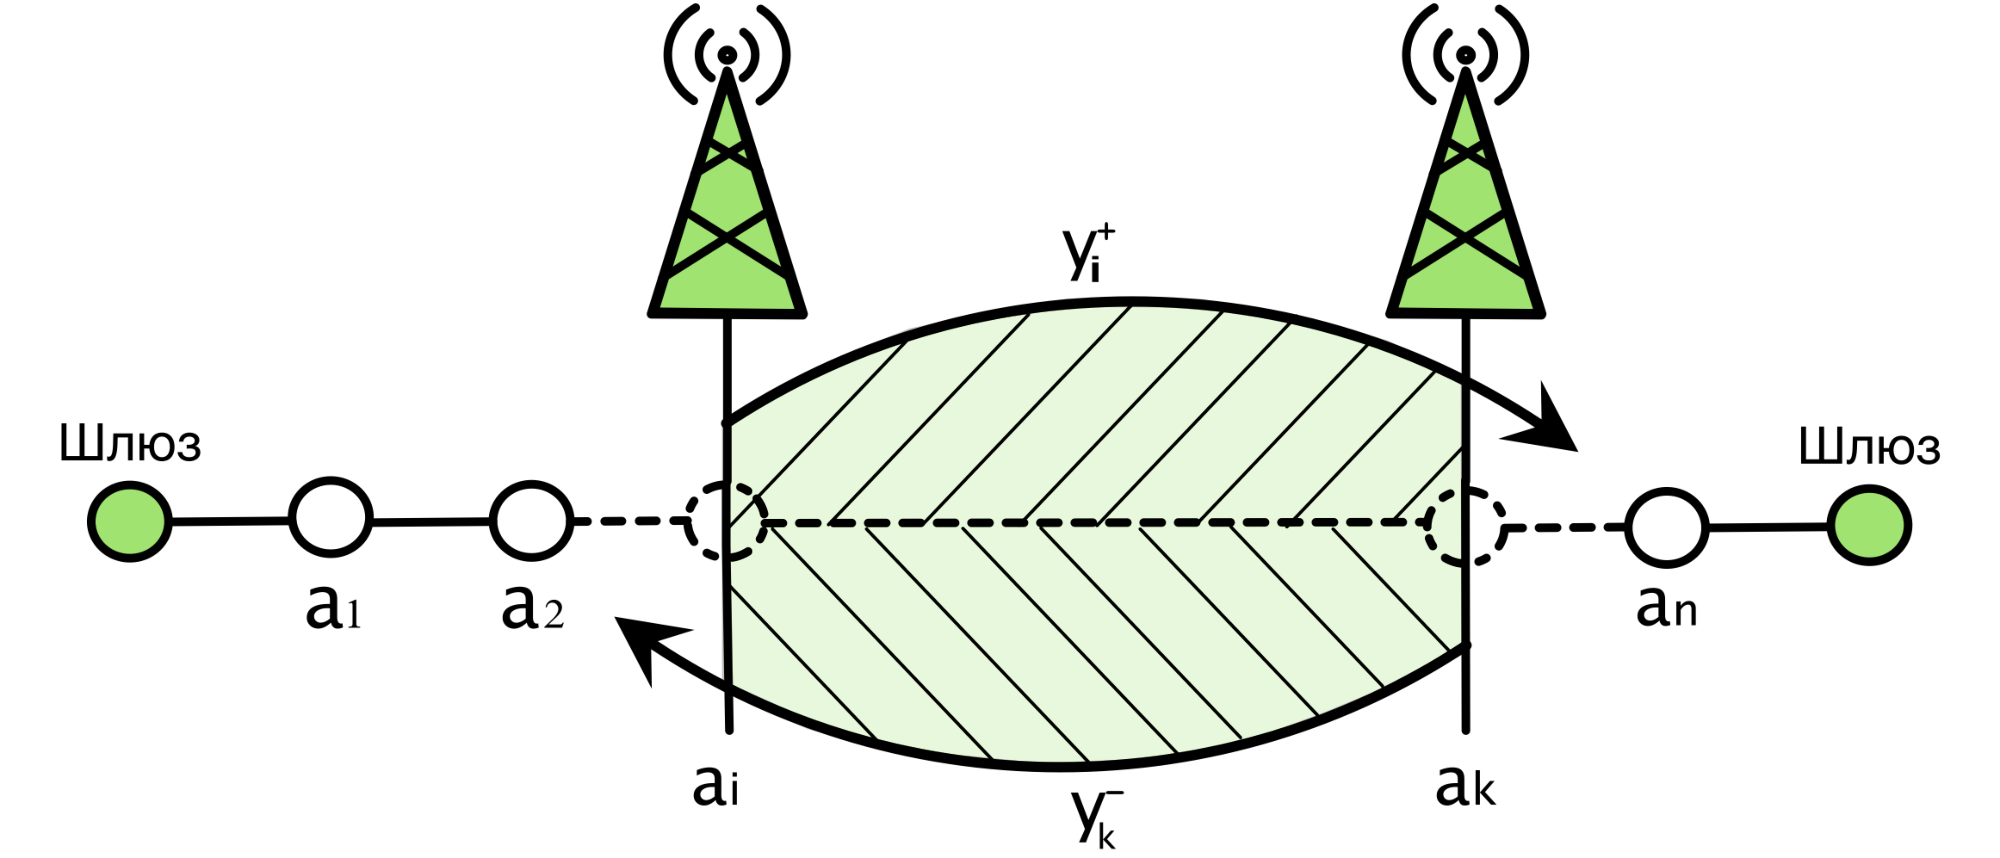
\includegraphics[scale=0.5]{total_coverage_between_points.pdf}
  }
  \caption{Область покрытия между любыми двумя точками}\label{fig:part3_total_coverage_between_points}
\end{figure}

Согласно условиям задачи, станция, расположенная в $ a_i $, должна быть связана хотя бы с одной станцией слева и одной станцией справа, включая станции на конечных точках $ a_0 $ и $a_{n + 1}$. 

Введем бинарные переменные $z_{ijkq}, i = \overline{1,n}; j= \overline{1,m}; k=\overline{1,n},  k \neq i; q= \overline{1,m}, q \neq j$.

Переменная $ z_ {ijkq} = 1$, если в точке $ a_i $ размещена станция $ s_j $ и данная станция связана со станцией $ s_q $, размещенная в точке $ a_k $; и $ z_ {ijkq} = 0 $ в противном случае.

Переменная $ z_{ij0(m + 1)} = 1$, если станция $ s_j $, размещенная в точке $ a_i $, связана со шлюзом $ s_{m + 1} $ в точке $ a_0 $; $ z_{ij0 (m + 1)} = 0 $ в противном случае.
 
Переменная $ z_{ij(n + 1)(m + 1)} = 1 $, если здесь находится станция $ s_j $ в точке $ a_i $ и она связана со шлюзом $ s_{m + 1} $ в точке $ a_{n + 1} $; $ z_{ij0(m + 1)} = 0 $  в противном случае.

Станции должны быть размещены в обеих точках $ a_i $ и $ a_k $, \cref{eq:part3_z_ijkq_1, eq:part3_z_ijkq_2}:

\begin{equation}
  \label{eq:part3_z_ijkq_1}
  z_{ijkq} \leq e_i , \quad i = \overline{1, n}; \quad j = \overline{1, m}; \quad k = \overline{1,n}, k \neq i; \quad q = \overline{1,m}, q \neq j;
\end{equation}


\begin{equation}
  \label{eq:part3_z_ijkq_2}
  z_{ijkq} \leq e_k , \quad k = \overline{1, n}; \quad j = \overline{1, m}; \quad i = \overline{1,n}, i \neq k; \quad q = \overline{1,m}, q \neq j.
\end{equation}


Необходимо, чтобы станция $ s_j $ в точке $ a_i $ была связана с  любой станцией, расположенной в точке $ a_k $, справа от $ a_i $ ($ k> i $) или с правым шлюзом $ s_{m + 1} $ \cref{eq:part3_z_ijkq_3_1, eq:part3_z_ijkq_3_2}. 

\begin{equation}
  \label{eq:part3_z_ijkq_3_1}
  \sum\limits_{k=i+1}^{n} \sum\limits_{\substack{q = 1\\ q \neq j}}^m z_{ijkq} + z_{ij(n+1)(m+1)} = x_{ij} ,  \quad i = \overline{1, n}, \quad j = \overline{1, m}.
\end{equation}


Станция $ s_j $, размещенная в $ a_{n} $, справа связана толко со шлюзом $ s_{m + 1} $ на месте $ a_ {n+1}$ \cref{eq:part3_z_ijkq_3_2}. 

\begin{equation}
  \label{eq:part3_z_ijkq_3_2}
  z_{nj(n+1)(m+1)} = x_{nj} \quad j = \overline{1, m}.
\end{equation}

Также станция должна быть связана с любой станцией, расположенной в точке $ a_k $ слева от точки $ a_i $ ($ k <i $) или с левым шлюзом $ s_{m + 1} $ \cref{eq:part3_z_ijkq_4_1, eq:part3_z_ijkq_4_2}.

\begin{equation}
  \label{eq:part3_z_ijkq_4_1}
  z_{1j0(m+1)}= x_{ij}, \quad j = \overline{1, m};
\end{equation}

Станция $s_j$, размещенная в точке $a_{1}$ слева может быть связана только со шлюзом $s_{m+1}$, расположенном в точке $a_0$ \cref{eq:part3_z_ijkq_4_1}.

\begin{equation}
  \label{eq:part3_z_ijkq_4_2}
  z_{ij0(m+1)} + \sum\limits_{k=1}^{i-1} \sum\limits_{\substack{q = 1\\ q \neq j}} z_{ijkq}= x_{ij}, \quad i = \overline{2, n}, \quad j = \overline{1, m}.
\end{equation}

Необходимо, чтобы станция $ s_q $ в точке $ a_k $ была связана с любой станцией справа, расположенной в точке $ a_i $ \cref{eq:part3_z_ijkq_5}.

\begin{equation}
  \label{eq:part3_z_ijkq_5}
  \sum\limits_{i=k+1}^{n} \sum\limits_{\substack{j=1 \\ j \neq q}}^m z_{ijkq} = x_{kq} , \quad k = \overline{1, n-1}, \quad q = \overline{1, m};
\end{equation}

Кроме того, станция $ s_q $ в точке $ a_k $ подключена к любой станции слева, расположенной в точке $ a_i $ \cref {eq:part3_z_ijkq_6}. 

\begin{equation}
  \label{eq:part3_z_ijkq_6}
  \sum\limits_{i=1}^{k} \sum\limits_{\substack{j=1 \\ j \neq q}}^m z_{ijkq} = x_{kq} , \quad k = \overline{2, n}, \quad q = \overline{1, m};
\end{equation}

Неравенства \cref{eq:part3_z_ijkq_1, eq:part3_z_ijkq_2} и равенства \cref{eq:part3_z_ijkq_3_1, eq:part3_z_ijkq_3_2, eq:part3_z_ijkq_4_1, eq:part3_z_ijkq_4_2, eq:part3_z_ijkq_5, eq:part3_z_ijkq_6} обеспечивают условие симметрии связи между базовыми станциями, расположенными в точках $ a_i $ и $ a_k $, $\forall i, k $ (Рис.\cref{fig:part3_station_link}).

\begin{figure}[ht]
  \centerfloat{
      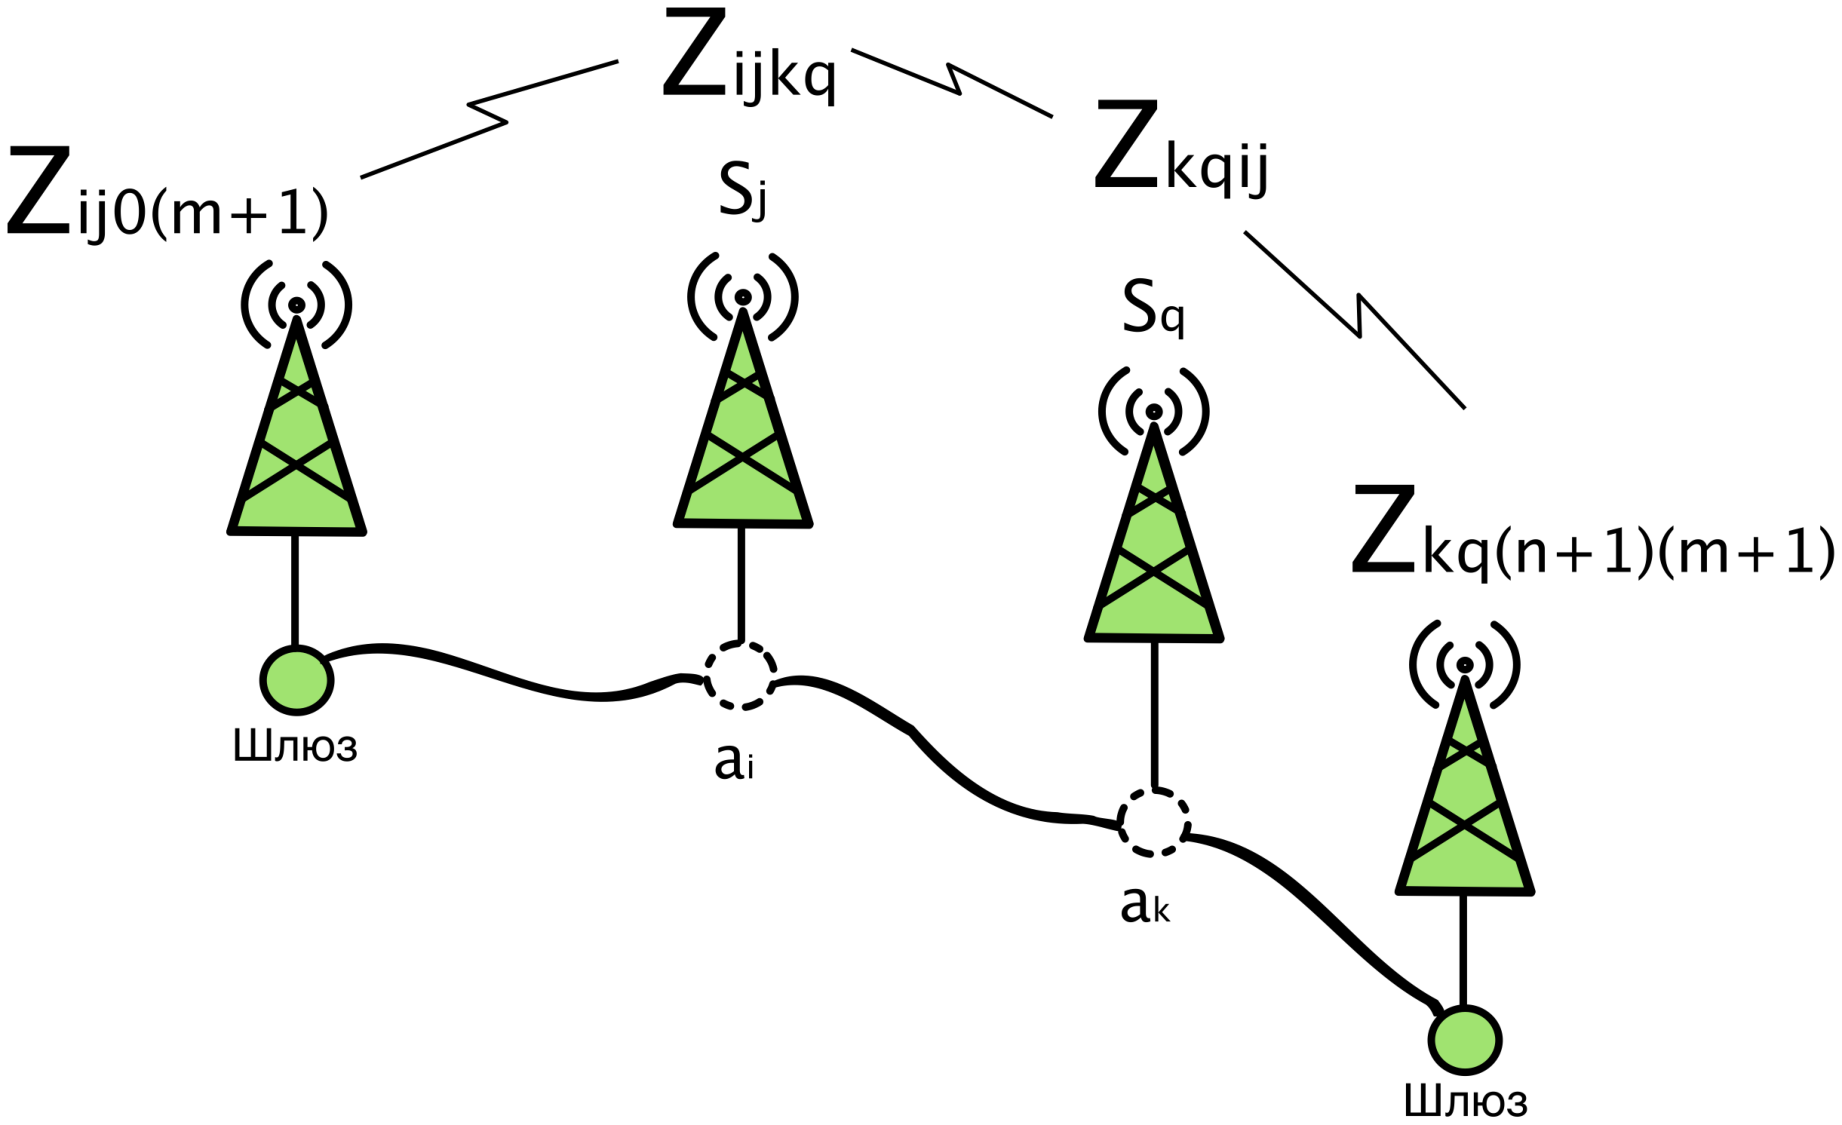
\includegraphics[scale=0.5]{station_link.pdf}
  }
  \caption{Связь между базовыми станциями}\label{fig:part3_station_link}
\end{figure}

Если станции $ s_j $ и $ s_q $ связаны, то максимальноый радиус связи размещенных станций должен быть не меньше расстояния между точками $ a_i $ и $ a_k $, где расположены станции $ s_i $ и $ s_q $ (Рис. \cref{fig:part3_station_link_between_points}). Формально это можно записать как \cref{eq:part3_z_ijkq_7, eq:part3_z_ijkq_8}.

 $\forall i= \overline{1,n}$:
\begin{equation}
  \label{eq:part3_z_ijkq_7}
  z_{ijkq}(R_{jq}-(a_i-a_k ))\geq 0, \quad k=\overline{0,i-1}; \quad j=\overline{1,m}; \quad q= \overline{1,m}, q \neq j; 
\end{equation}

\begin{equation}
  \label{eq:part3_z_ijkq_8}
  z_{ijkq} (R_{jq}-(a_k-a_i )) \geq 0, \quad k=\overline{i+1,n+1}; \quad j=\overline{1,m}; \quad q= \overline{1,m}, q \neq j.
\end{equation}

\begin{figure}[ht]
  \centerfloat{
      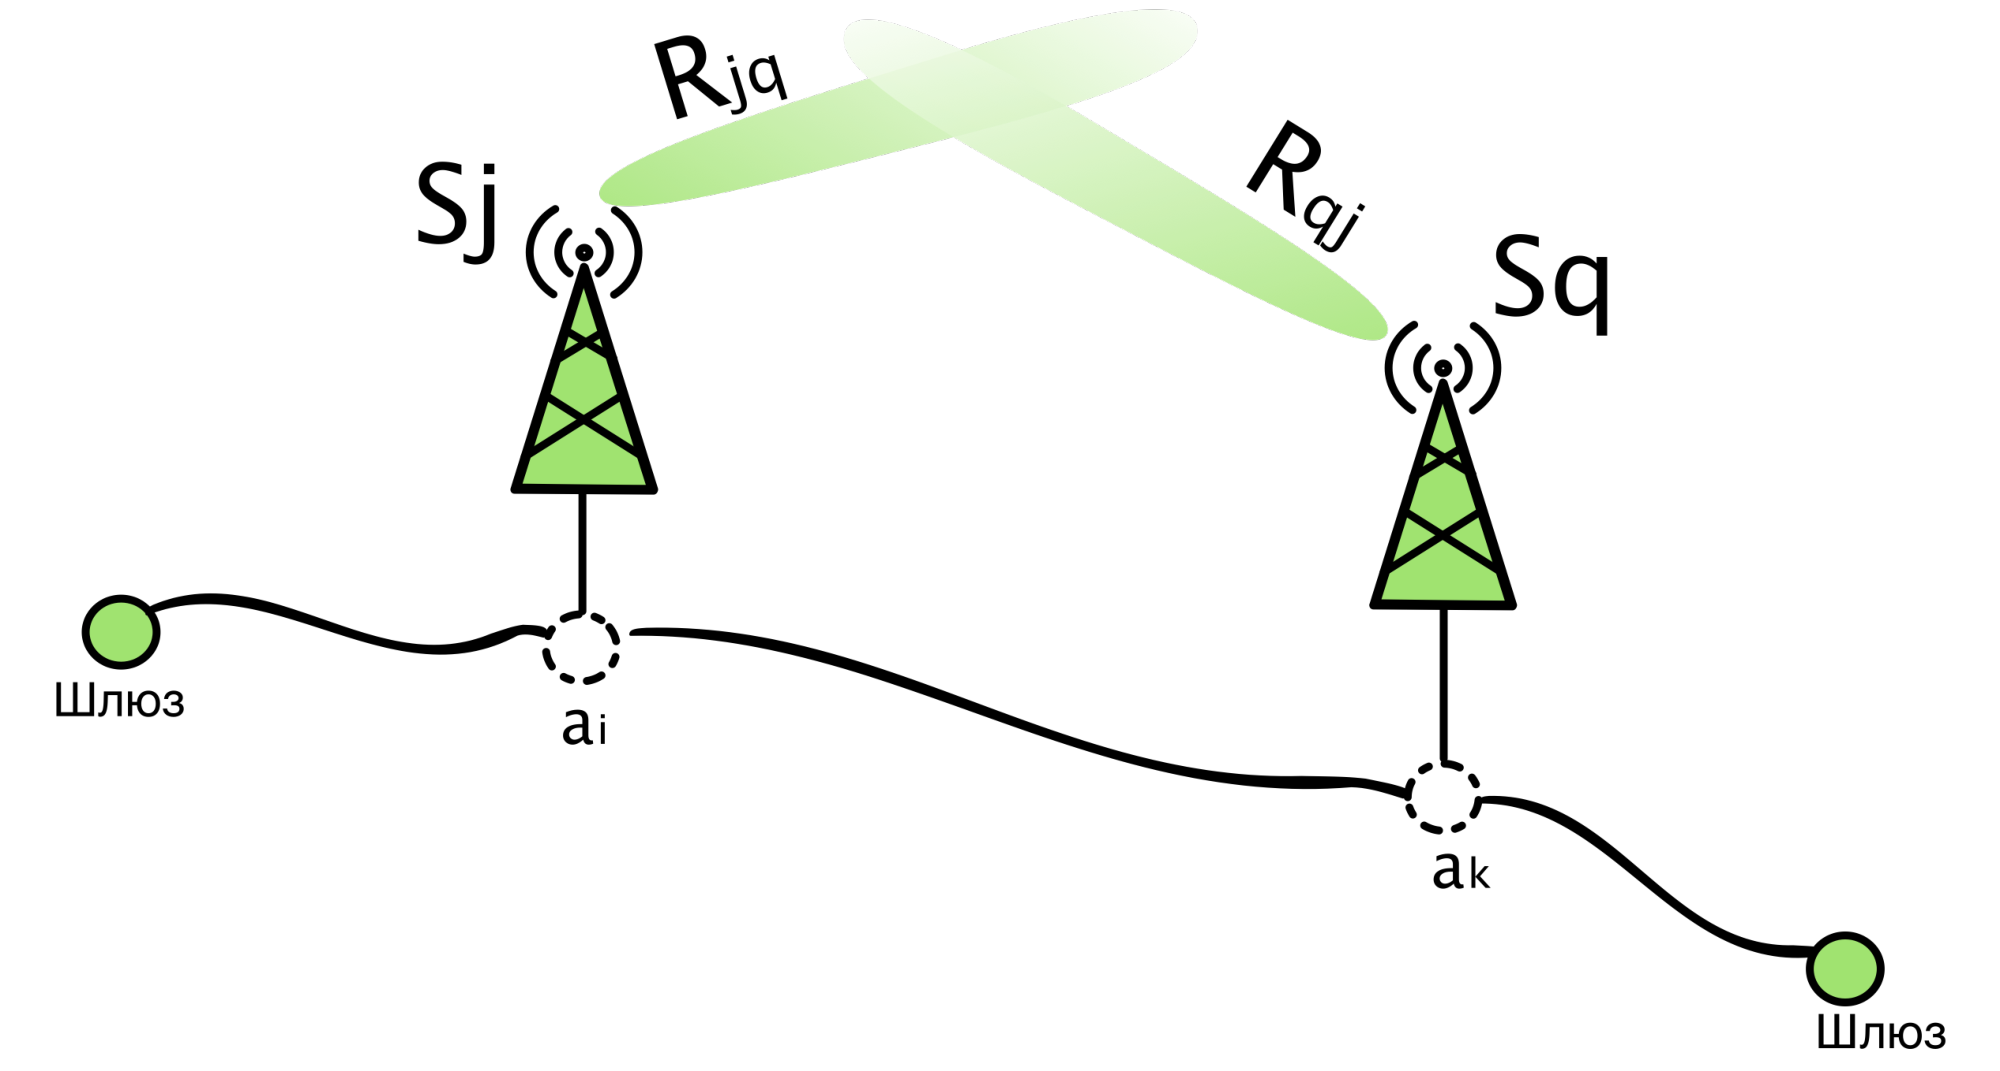
\includegraphics[scale=0.5]{station_link_between_points.pdf}
  }
  \caption{Обеспечение связи с соседней станцией}\label{fig:part3_station_link_between_points}
\end{figure}

И для бюджетного ограничения стоимости $C$:

\begin{equation}
  \label{eq:part3_cost}
  \sum\limits_{i=1}^n \sum\limits_{j=1}^m x_{ij} \cdot c_j \leq C.
\end{equation}

Работа \cite{Ivanov2018} содержит доказательство NP-трудности для частного случая задачи ЦЛП, когда вдоль линейной территории размещают множество однотипных станций с одинаковыми параметрами. Представленная в данном исследовании модель \cref{eq:part3_objective_function} -- \cref{eq:part3_cost} рассматривает общий случай размещения, когда вдоль линейного участка размещают множество различных станций с разными техническими параметрами. Следовательно, данная задача является также NP-трудности.

Представленная математическая модель рассчитывалась в пакете Optimization Toolbox MATLAB.Числовой пример решения полученной матемаческой модели задачи ЦЛП представлен в приложении \cref{app:ilp_solution}. В приложении также представлена методика расчета дальности связи для обеспечения коммуникации между базовыми станциями и охвата зоны покрытия.

% \section{Численный пример}
% В этой секции представлен численный пример решения данной задачи.
% % This section shows one simple case of the problem.

% Задан линейный участок $L$ с длиной 300 с количеством $n=7$ точек размещения. Координаты точек размещения представлены в таблице \cref{tab:part3_placed_point}.  Задан бюджет размещения $C=130$. Центарльная частота $f = 2437$ МГц. 

% \begin{table}[h!]\centering
%   \begin{tabular}{|c||c|c|c|c|c|c|c|}\hline
%     $a_i$ & $a_1$ &  $a_2$ & $a_3$ & $a_4$ & $a_5$ & $a_6$ & $a_7$ \\ \hline \hline
%     Координата & 29 & 40 & 95 & 139 & 181 & 230 & 273 \\ \hline
% \end{tabular}\caption{Точки размещения участка с длиной $L = 300$.}\label{tab:part3_placed_point}
% \end{table}

% Задано множества базовых станций $m = 8$ с параметрами представленными в таблице \cref{tab:part3_BS}. Также в таблице представлены параметры шлюзов и контролируемых объектов. Параметры объектов необходимы для расчета радиусов покрытия станций.

% \begin{table}[b]\centering
%   \begin{tabular}{|c||c|c|c|c|c|c|c|}\hline
%     BS & $P_{tr}^R$ &  $G_{tr}^R$ & $P_{recv}^R$ & $P_{recv}^r$ & $G_{recv}^r$ & $c$ \\ \cline{2-1} \cline{3-1} \cline{4-1} \cline{5-1}  \cline{6-1} \cline{7-1}
%      & дБм & дБ & Дбм & дБм & дБ & у.е.  \\ \hline
%     1 & 20 & 5 & -69 & -67 & 5 & 40 \\ 

%     2 & 19 & 5 & -67 & -67 & 5 & 28 \\ 

%     3 & 18 & 5 & -69 & -67 & 5 & 45 \\ 

%     4 & 19 & 5 & -69 & -67 & 6 & 22 \\ 

%     5 & 19 & 5 & -67 & -67 & 5 & 21 \\ 

%     6 & 20 & 5 & -69 & -67 & 5 & 40 \\ 

%     7 & 19 & 5 & -67 & -67 & 5 & 28 \\

%     8 & 18 & 5 & -69 & -67 & 5 & 45 \\ \hline \hline  

%     &  $G_{recv}^R$ & $P_{recv}^R$ &  & & $P_{tr}^r$ & $G_{tr}^r$ \\  \cline{2-1} \cline{3-1} \cline{6-1} \cline{7-1} 

%     Шлюз& дБ & дБм & & Объект & дБм & дБ  \\  \cline{2-1} \cline{3-1}  \cline{6-1} \cline{7-1}

%     &  5 & -69 & &  & 15 & 2  \\ \hline

%   \end{tabular}\caption{Параметры базовых станций, шлюзов и объектов.}\label{tab:part3_BS} 
% \end{table}

% \subsection{Расчет радиса связи между станциями}
% Базовые станции оснащены направленной антенной с высоким коэффициентом усиления для связи с соседними станциями.
% Для расчета потерь между станциями $j$ и $q$ воспользуемся формулой (\ref{eq:part3_L_fs_from_link_budget}):

% \begin{displaymath}
%   L_{fs}^{jq} = P_{tr}^R(j) - L_{tr} + G_{tr}^R(j) + G_{tr}^R(q) - L_{recv} - SOM - P_{recv}^R(q).
% \end{displaymath}


% Потери на кабелях приемникп $ L_{recv} $ и передатчике $ L_{tr} $ примем равным 1 дБ и запас на замирания сигнала $ SOM = 10 $ дБ.

% Let us carry out an example of the calculation communication link between stations $ s_1 $ and $ s_2 $:
% Для примера расчетаем радиус связи между станциями $ s_1 $ и $ s_2 $:

% \begin{align}
%   \begin{aligned}
%   L_{fs}^{12} = P_{tr}^R(1) - L_{tr} + G_{tr}^R(1) + G_{tr}^R(2) - L_{recv} - SOM - P_{recv}^R(2)= \\
%   = 20 - 1 + 5 + 5 - 1 - 10 - (-69) = 87 (dB).
%   \end{aligned}
% \end{align}

% Для расчета канала связи необходимо использовать формулу \cref{eq:part3_D}. Несущая частота $ f = 2437 $ МГц и коэффициент для расчета потерь $ K = -27,55 $:

% \begin{align}
%   \begin{aligned}
%   R_{jq} = 10^{\left(\frac{L_{fs}^{jq} - 20\lg{F} - K}{20}\right)}
%   = 10^{\left(\frac{87 - 20\lg{2437} - (-27.55)}{20}\right)} = 174 (m).
%   \end{aligned}
% \end{align}

% В таблице \cref{tab:part3_Rjq} приведены расчеты максимальных радиусов связи между всеми станциями $ s_j $, $ j = 1, ..., m $ и шлюзом $ s_ {m + 1} $.

% \begin{table}[h!]\centering
%   \begin{tabular}{|c||c|c|c|c|c|c|c|c|c|}\hline
%       $R_{jq}, (m)$ & $s_1$ & $s_2$ & $s_3$ & $s_4$ & $s_5$ & $s_6$ & $s_7$ & $s_8$ & $s_{m+1}$ \\ \hline \hline

%       $s_1$ &--& 174& 219& 219& 174& 219& 174& 219& 219\\ 
%       $s_2$ &195& --& 195& 195& 155& 195& 155& 195& 195\\ 
%       $s_3$ &174& 138& --& 174& 138& 174& 138& 174& 174\\ 
%       $s_4$ &195& 155& 195& --& 155& 195& 155& 195& 195\\ 
%       $s_5$ &195& 155& 195& 195& --& 195& 155& 195& 195\\ 
%       $s_6$ &219& 174& 219& 219& 174& --& 174& 219& 219\\
%       $s_7$ &195& 155& 195& 195& 155& 195& --& 195& 195\\ 
%       $s_8$ &174& 138& 174& 174& 138& 174& 138& --& 174\\ 
%       \hline

% \end{tabular}\caption{Рассчитанные радиусы связи между станциями}\label{tab:part3_Rjq}
% \end{table}

% \subsection{Расчет радиуса покрытия}

% % Для покрытия заданного участка базовая станция оснащена всенаправленной антенной с выходной мощностью $ P_{tr}^r $ и усилением $ G_{tr}^r$. Потери в кабеле $ L_ {tr} $ равно 1.

% % To cover a given section, the base station is equipped with an isotropic antenna with output power $ P_ {tr} ^ r $ and gain $ G_ {tr} ^ r $ is equal to 0. The cable loss $ L_ {tr} $ is equal to 1.

% % A coverage area depends on a base station, as well as user device characteristics. Let us consider a user device with an antenna sensitivity $P_{RX} = -67$ dBm and gain $G_{RX} = 0$. Loss $L_{RX}$ is equal to 0.
% Расчет проводится аналогично расчета радиусу связи между станциями. 
% Потери в свободном простанстве для канала между $j$-ой станции и контролируемым объектом

% \begin{displaymath}
%   L_{fs}^{j} = P_{tr}^r(j) - L_{tr}  - SOM - P_{RX}. 
% \end{displaymath}


% Пример расчечта радиуса покрытия для  $1$-ой станции:

% \begin{displaymath}
%   L_{fs}^{1} = P_{tr}^r + G_{tr}^r + G_{recv}^r(1) - L_{recv}(1)  - SOM - P_{recv}^r(1) = 15+2+5-1-(-67)-10 = 78 \text{ (дБ)}.
% \end{displaymath}

% \begin{displaymath}
%   r_{1} = 10^{\left(\frac{78 - 20\lg{2437} - (-27.55)}{20}\right)} = 77 \text{ (м)}.
% \end{displaymath}

% Рассчитанные радиусы покрытия для всех станций $ s_j $, $ j = \overline{1, m} $ представлены в таблице \cref{tab:part3_rj}).

% \begin{table}[h!]\begin{center}
%   \begin{tabular}{|c||c|c|c|c|c|c|c|c|}\hline
%       STA & $s_1$ & $s_2$ & $s_3$ & $s_4$ & $s_5$ & $s_6$ & $s_7$ & $s_8$\\ \hline \hline

%       $r_{j}$ & 77 & 77 & 77 & 87 & 77 & 77 & 77 & 77\\ \hline

% \end{tabular}\caption{Рассчитанные радиусы покрытия станций}\label{tab:part3_rj}
% \end{center}\end{table}

% Задача ЦЛП решена с помощью Optimization Toolbox MatLab. Таблица \cref{tab:part3_ilp_solution} содержит все возможные целочисленные решения.

% \begin{table}[h!]\centering
%   \begin{tabular}{|c||c|c|c|c|c|c|c||c|c|}\hline
%     $a_i$ & $a_1$ &  $a_2$ & $a_3$ & $a_4$ & $a_5$ & $a_6$ & $a_7$  & Покрытие & Цена \\ \hline 
%     Координаты & 29 & 40 & 95 & 139 & 181 & 230 & 273 & м & у.е.\\ \hline \hline
%     Целлочисленное решение 1 & $s_1$ & $s_2$ & $s_6$ & -- & -- & -- & $s_4$ & 286 & 130\\ 
%     Целлочисленное решение 2 & $s_4$ & -- & $s_5$ & $s_7$ & -- & -- & $s_2$ & 289 & 99\\
%     Оптимальное решение & $s_4$ & $s_2$ & -- & -- & $s_1$ & -- & $s_5$ & 300 & 111 \\ \hline
% \end{tabular}\caption{Решение задачи ЦЛП.}\label{tab:part3_ilp_solution}
% \end{table}

% \chapter{Математические модели синтеза топологии сети для охвата линейного участка в виде экстремальной задачи в комбинаторной форме}\label{chapter_combinatorial_model}

\section{Математические модели синтеза топологии сети для охвата линейного участка в виде экстремальной задачи в комбинаторной форме}

Эффективным способом повышения технико-экономических показателей при проектировании \fixme{БШС} является оптимизация топологии сети, а именно решение задачи выбора оптимального набора станций из заданного избыточного множества и определение мест их размещения вдоль линейной контролируемой территории.
Основным результатом работы, представленной в этой главе, является разработка итерационного метода выбора оптимальной топологии сети в процессе комплексного проектирования БШС. 
Принципиальной особенностью предлагаемого метода, повышающей его эффективность, является то, что для рассмотрения на этапе моделирования предлагается не одно решения, а последовательности лучших решений задачи оптимизации топологии сети. Это позволяет с помощью разработанной итерационной процедуры выбирать на этапе моделирования лучшее решение среди тех решений по топологии, которые удовлетворяют требуемым характеристикам проектируемой БШС. 

\subsection{Постановка задачи и ее формулировка в экстремальной комбинаторной форме}

Пусть задано множество станций $S=\{s_j\}$ с параметрами $s_j=\{r_j,\{R_{jq} \},\mu_j, c_j \},j=1,...,m;q=1,...,m;j \neq q $. Здесь $r_j$ -- максимальный радиус покрытия станции, $\{R_{jq} \}$ -- множество максимальных радиусов связи между $j$-ой и $q$-ой базовой станции, $\mu_j$ - интенсивность времени обслуживания и $c_j$ -- стоимость станции.

Задана максимальная допустимая стоимость размещенных станций $C$. 


Задан отрезок $\alpha$ длиной $L$ с концами в точках $a_0$ и $a_{n+1}$. Внутри отрезка $\alpha = [a_0, a_{n+1}]$ задано множество возможных точек размещения станций множества $A=\{a_i \},i=1,...,n$ c координатами $l_i$.Точка $a_0$ имеет координату $l_0=0$, точка $a_{n+1}$ имеет координату $l_{n+1}=L$. На концах отрезка, в вершинах $a_0$ и $a_{n+1}$, стоят станции специального вида $s_0$ и $s_{m+1}$, соответственно, для которых радиусы покрытия, пропускные способности и стоимости не задаются. Радиусы связи задаются как $R_{0j}$ и $R_{(m+1)j}$, соответственно.
Требуется разместить станции таким образом, чтобы максимизировать размер контролируемой ими территории (покрытие) отрезка $L$ при выполнении требования наличия связи каждой станции со станциями на концах отрезка (шлюзами) через систему размещенных станций при выполнении ограничений на время межконцевой задержки $T$ и суммарную стоимость размещенных станций $C$.
Сформулируем задачу в виде экстремальной задачи на конечном множестве.

\textit{Допустимой расстановкой станций} назовем такой возрастающий по величине координат $l_i$  набор пар $P = \{a_i, s_j\},a_i \in A,i \neq 0,i \neq n+1;s_j \in S$, для которого выполняются требования:

% \begin{enumerate}
% 	\item left connectivity: $\forall\;(a_i, s_j),\,1 \leq i \leq n,$ either $\exists (a_k, s_q):\:l_k < l_i $ 
% 	and $l_i - l_k \leq \min \{R_j, R_q \},$ or $l_i - l_0 \leq R_j$;
% 	\item right connectivity: $\forall\;(a_i, s_j),\,1 \leq i \leq n,$ either $\exists (a_t, s_g):\:l_t > l_i $ 
% 	and $ l_t - l_i \leq \min \{R_j, R_g \}, $ or $ l_{n+1} - l_i \leq R_j$;	
% 	\item $|P| = m$.
% \end{enumerate}
\begin{enumerate}
    \item  для каждой пары $(a_i,s_j)$:
        \begin{enumerate}
            \item слева: либо найдется такая пара $(a_k,s_q)$, что, $l_i - l_k \leqslant R_{jq}$  и $l_i - l_k  \leqslant R_{qj}$, либо $l_i-l_0 \leqslant R_{j0}$ и $l_i - l_0 \leqslant R_{0j}$;
            \item справа: либо найдется такая пара $(a_t,s_g)$, что, $l_t-l_i \leqslant R_{jq}$ и $l_t - l_i \leqslant R_{qj}$, либо $l_{n+1}-l_i \leqslant R_{j(m+1)}$ и $l_{n+1}-l_i \leqslant R_{(m+1)j}$. 
  \end{enumerate}
% - слева: либо найдется такая пара (a_k,s_q), что, l_i-l_k≤R_jq  и l_i-l_k  ≤R_qj, либо l_i-l_0≤R_j0 и l_i-l_0≤R_0j;
% - справа: либо найдется такая пара (a_t,s_g), что, l_t-l_i≤R_jq и l_t-l_i  ≤R_qj, либо l_(n+1)-l_i≤R_(j(m+1)) и l_(n+1)-l_i≤R_((m+1)j). 
Данное требование гарантирует, что любая станция может быть связана со станциями на концах отрезка либо через промежуточные станции, либо непосредственно;
    \item в одной точке стоит не более одной станции;
    \item сумма задержек по всем размещенным станциям меньше заданной величины $T$ – средней межконцевой задержки по времени по всей системе станций:
    \begin{displaymath}
        \label{eq:part3_e2e_delay}
        \sum\limits_{j \in S_\sigma} \overline{T_j} \leqslant T,
    \end{displaymath}
где $S_\sigma$ – множество размещенных станций, $\overline{T_j}$ -- среднее время задержки на станции. Расчет задержек описан в параграфе \cref{part4_e2e_delay_section}
    \item суммарная стоимость размещенных станций меньше заданного бюджетного ограничения  $C$.
\end{enumerate}

Каждой допустимой расстановке станций $P$ соответствует величина покрытия $z(P)$, определяемая как суммарная длина всех таких участков $\tau,\tau \subset \alpha$, что каждая точка этих 
участков попадает в зону покрытия, по крайней мере, одной станции, входящей в набор пар $P$.

Для удобства описании в дальнейшем алгоритмов введем понятие «недопокрытия» отрезка $\alpha$:

\begin{displaymath}
    f(P) = L - z(P)
\end{displaymath} 

Пусть $G$ -- множество всех допустимых расстановок $P$.
Тогда мы можем сформулировать нашу задачу в следующей комбинаторной форме экстремальной задачи на конечном множестве. 

\textbf{Задача 1.}

Требуется найти такую допустимую расстановку  $P^*$, что
\begin{equation}
    \label{eq:part3_P}
    P^* = \argmin \limits_{P \in G} f(P)
\end{equation}

Обозначим через $\Gamma$ все множество вариантов размещения станций (не обязательно допустимых) из множества $S$ на заданном множестве возможных мест их размещения.

\subsection{Дерево ветвлений для перебора элементов в множестве \texorpdfstring{$\Gamma$}{Lg}}

Опишем процедуру построения бинарного дерева поиска (дерева ветвлений) для полного перебора без повторений всех элементов множества $\Gamma$. Данная процедура будет использована в дальнейшем при построении дерева поиска в алгоритме МВиГ решения \textbf{задачи 1} \cite{SigalBook}.

Будем предполагать, что в множестве $S$ станции упорядочены по не убыванию радиусов покрытия.


Описываемая процедура использует известный прием разбиения множества $G$ на подмножества с использованием некоторого параметра. Процесс формирования и последовательность исследования подмножеств обычно представляется с помощью дерева поиска, представляющего собой ориентированное от корня «дерева ветвлений», где каждому подмножеству соответствует вершина на дереве. Множеству $\Gamma$ соответствует корневая вершина. 

\paragraph{Параметр для разбиения множеств на подмножества}


\paragraph{\textit{\textbf{Процедура 1.}}}

Выбор способа ветвления дерева связан со спецификой задачи. В случае \textbf{задачи 1} спецификой является размещение множества станций $S$ на множестве возможных точках размещения $A$. На каждом узле дерева будем применять дихотомическое ветвление.

Пусть $G_0$, где нижний индекс – номер итерации, исходного множества $\Gamma$. На каждой итерации, начиная с итерации $\nu=0$, разбиваем текущее подмножество $G_\nu$ на два подмножества $G^1_\nu$ и $G^2_\nu$. При этом множество $G_\nu$ обычно называется «материнским», а множества $G^1_\nu$  и $G^2_\nu$  - «потомками» множества $G_\nu$ или дочерними узлами.

В качестве параметра разбиения воспользуемся переменной $\pi_{ij}$, принимающей два значения 0 и 1:

\begin{itemize}
    \item $\pi_{ij}=1$, если наложено условие, что на месте $a_i$ расположена станция $s_j$;
    \item $\pi_{ij} = 0$, если наложено условие, что на месте $a_i$ станция $s_j$  располагаться не будет.
\end{itemize}

В дальнейшем будем считать, что для множества $G^1_\nu$ задано условие $\pi_{ij}=1$, а для множества $G^2_\nu$  задано условие $\pi_{ij} = 0$.

Очевидно, что

\begin{equation}
    \label{eq:part4_G_cup}
    G^1_\nu \cup G^2_\nu = G_\nu;
\end{equation}


\begin{equation}
    \label{eq:part4_G_cap}
    G^1_\nu \cap G^2_\nu = \varnothing.
\end{equation}

Выбор переменной для разбиения на $\nu$-ой итерации

На этапе разбиения любого множества $G_\nu$ все множество переменных $\Pi = \{\pi_{ij}\}$ можно разделить на три подмножества: множество $\Pi^+$ -- «фиксированные» переменные, для которых $\pi_{ij}=1$, множество $\Pi^-$ -- «запрещенные» переменные, для которых $\pi_{ij}=0$, и множество $\Pi^f$ -- «свободные» переменные, для которых значения на данной итерации еще не заданы.

Правило выбора переменной для разбиения множества $G_\nu$. Для разбиения множества $G_\nu$ на данной итерации выбирается из множества $\Pi^f$ переменная c наименьшим индексом $j$ среди всех переменных с наименьшим индексом $i$. Таким образом сначала определяется незанятое место размещения $a_i$ с наименьшим номером (индексом $i$) и на нем размещается еще не размещенная станция $s_j$ с наименьшим номером (индексом $j$).

\paragraph{Движение по дереву ветвлений.}

После разбиения очередного подмножества $G_\nu$ два подмножества $G^1_\nu$  и $G^2_\nu$, последним на дереве ветвлений присваиваются порядковые индексы $G_{\nu+1}$ и $G_{\nu+2}$, соответственно.
При формировании дерева ветвлений различаются два типа шагов: «прямой» шаг и «обратный» шаг. Прямой шаг -- это движение «в глубину» по той же ветви дерева, реализующее очередное разбиение множества $G_\nu$ на два потомка, и обратный шаг, реализующий переход от множества $G_\nu$  к одному из ранее сформированных подмножеств. Обратный шаг делается в том случае, когда либо получено множество $G_\nu$, состоящее из единственного элемента, либо множество $G_\nu$  при данном наборе значений переменных $\pi_{ij}$, выделяющих данное подмножество $G_\nu$ из множества $G_0$, пусто. В этих случаях соответствующая вершина дерева называется «закрытой».

Для движения по дереву будем использовать правило \fixme{LIFO}. На основании этого правила прямые шаги будут выполняться до тех пор, пока не будет получена закрытая вершина. На дереве ветвлений это соответствует продолжению движения по той же ветви дерева. При этом из двух множеств $G^1_\nu$  и $G^2_\nu$ первым будет исследоваться на возможность закрытия соответствующей вершины множество $G^1_\nu$. Если вершина в результате проведенного исследования не будет закрыта, то из неё будет продолжено дальнейшее движение по той же ветви (выполнение прямого шага). Если вершина будет закрыта, то будет выполнен обратный шаг: для дальнейшего рассмотрения и продолжения движения будет выбрана незакрытая вершина с наибольшим порядковым номером $\nu$ среди всех висячих вершин дерева (последняя сформированная вершина из нерассмотренных). Процедура будет завершена, когда все вершины дерева будут закрыты.

Заметим, что выполнение условий \cref{eq:part4_G_cup, eq:part4_G_cap} гарантирует, что в результате завершения работы \textit{\textbf{процедуры 1}} будут просмотрены все элементы множества $\Gamma$ без повторений. Эти же условия определяют фундаментальное свойство дерева ветвлений: на каждой итерации объединение множеств $G_\nu$ всех висячих вершин дерева дает исходное множество $G_0$ корневой вершины.


\paragraph{Алгоритм метода ветвей и границ} \label{BnB}
Для построения алгоритма \fixme{МВиГ} для решения \textbf{задачи 1} с использованием \textit{\textbf{процедуры 1}} для построения дерева ветвлений нам достаточно разработать методы исследования вершин дерева на возможность их закрытия.
В соответствии с техникой \fixme{МВиГ} закрытие вершины в результате исследования, соответствующего ей множества $G_\nu$ возможно в трех случаях.

\underline{\textit{\textbf{Случай 1.}}} Множество $G_\nu$ -- пусто, т.е. доказано, что в множестве $G_\nu$ при данном наборе фиксированных и запрещенных переменных $\pi_{ij}$ нет ни одной допустимой расстановки $P$.

\underline{\textit{\textbf{Случай 2.}}} Доказано, что в множестве $G_\nu$ не может быть допустимой расстановки P с меньшим значением целевой функции (1), чем у лучшей расстановки $\widehat{P}$ из уже найденных. Значение функции $f(\widehat{P})$ называется «рекордом», а расстановка $\widehat{P}$ -- «рекордным решением». В качестве начального рекорда принимается число заведомо большое искомого оптимального решения, например, $L$ – длина всего отрезка.

\underline{\textit{\textbf{Случай 3.}}} Найдено оптимальное решение \textbf{задачи 1} на множестве $G_\nu$.
Прежде чем рассмотреть эти три случая, запишем важное свойство любого множеств $G_\nu$, являющееся следствием принятого правила выбора свободной переменной для разбиения очередного множества $G_\nu$ при прямом шаге. 

\textit{\textbf{Свойство 1.}} Пусть для исследуемого множества $G_\nu, \nu > 0$, точка $a_k$ -- это одно любое из мест, на которых уже размещены станция из множества $S$ в соответствии с набором фиксированных и запрещенных переменных $\pi_{ij}$, выделяющим данное множество из множества $G_0$. Тогда для всех мест «слева» от $a_k$, т.е. точек $a_i$, $i<k$, размещение станций уже определенно (при этом некоторые места могут быть пустыми).
Перейдем непосредственно к исследованию \underline{\textit{\textbf{случаев 1 – 3}}}.

\underline{\textit{\textbf{Случай 1.}}}

Проверка текущего множества $G_\nu$ на пустоту состоит в установлении факта невозможности выполнения требований 1) – 4) введенных ранее при определении допустимой расстановки.

Рассмотрим проверку условия выполнения требования 1) для множества $G_\nu, \nu > 0$. 

Пусть множество $G_\nu$  образовано разбиением материнского множества при помощи переменной $\pi_{kt}=1$. Проверяем, что каждый из радиусов $R_{th}$ и $R_{ht}$, где $h$ – индекс станции, размещенной на ближайшей слева к точке $a_k$ точке $a_d$ больше расстояния $l_k-l_d$. Если ближайшая слева точка – это точка $a_0$ (левый конец отрезка $\alpha$), то делается проверка, для радиуса $R_{t0}$ и $R_{0t}$. 

Если данное условие не выполняется, то множество $G_\nu$ недопустимо, соответствующая вершина закрывается и делается шаг обратного хода в соответствии с \textit{\textbf{процедурой 1}}. 

Если множество $G_\nu$ образовано разбиением материнского множества при помощи переменной $\pi_{kt}=0$ и $a_d$ -- точка с наибольшим индексом, среди точек, на которых уже размещены станции (точки $a_0$, если размещенных станций нет), то надо проверить, что среди нераспределенных станций, без учета станции $s_t$, есть такая станция $s_q$ что расстояние между точками $a_k$ и $a_d$ не больше, чем $R_{qh}$ и $R_{hq}$. Если проверка отрицательна, то множество $G_\nu$ -- пусто, соответствующая этому множеству на дереве поиска вершина должна быть закрыта и выполняется шаг обратного хода в соответствии с  \textit{\textbf{процедурой 1}}.

Требование 2) выполняется соответствующим выбором очередной станции для размещения, требования 3) и 4) выполняются непосредственным суммированием соответствующих параметров у размещенных станций.

\underline{\textit{\textbf{Случай 2.}}}
Построим оценку величины «недопокрытия» для множества $G_\nu$, полученного из материнского множества добавлением условия $\pi_{kt}=1$. Частичным «недопокрытием» назовем величину $\Delta(k,d,p,t)$, которая вычисляется по формуле:

\begin{equation}\label{eq:part4_delta}
\Delta(k,d,p,t) = max\{\left(a_{k} - a_{d} \right) - \left(r_{p} + r_{t} \right), 0\}.
\end{equation}

Частичное «недопокрытие» \cref{eq:part4_delta} определяется для любых двух точек $a_d$ и $a_k$,$k>d$, на которых расположены станции $s_p$ и $s_t$ при условии, что между этими точками нет других станций. Очевидно, что для любой расстановки $P$ «недопокрытие» $f(P)$ вычисляется как сумма всех «недопокрытий» $\Delta(k,d,p,t)$ между местами размещения станций, включая концы отрезка $\alpha$, на которых стоят станции особого типа $s_0$ и $s_{m+1}$.

Построим нижнюю оценку $W(G_{\nu} )$ для недопокрытий $f(P)$ расстановок $P$ множества $G_\nu$, т.е. 

\begin{displaymath}
W(G_\nu) \leq f(P), P \in G_\nu. 
\end{displaymath}

Если $W(G_\nu) \geq f(\widehat{P})$, то множество $G_\nu$ не может содержать расстановки лучше уже найденной расстановки $\widehat{P}$ соответствующая множеству $G_\nu$  вершина на дереве поиска должна быть закрыта и далее выполняется шаг обратного хода в соответствии с  \textit{\textbf{процедурой 1}}. 

Построим оценку «недопокрытия» для множества $G_\nu$, полученного из материнского множества добавлением условия $\pi_{kt}=1$. Оценку будем искать в виде суммы

\begin{displaymath}
    W\left(G_\nu\right) = w_1 + w_2. 
\end{displaymath}

Величина $w_1 \left(G_\nu \right)$ вычисляется как сумма все частичных «недопокрытий» слева от вершины $a_k$ и величины радиуса покрытия, размещаемой станций $r_t$. Оценку $w_2 \left(G_\nu \right)$ вычислим «для недопокрытия» справа на части $\beta$ до конца отрезка $\alpha$ (точки $a_{n+1}$). Данную оценку получим релаксацией условий, определяющих допустимую расстановку станций на участке $\beta$. Найдем такое подмножество $S_\beta$ множества станций $S$, состоящее из еще не размещенных станций и дающее минимальное «недопокрытие» на участке $\beta$ при выполнении только условий 2) – 4). Для этого сформулируем следующую задачу булевого программирования.

\underline{\textit{\textbf{Задача 2.}}}
\begin{displaymath}
    z = |\beta| - \sum\limits_{x_j \in S_\beta} r_j x_j \rightarrow min.
\end{displaymath}
при условии:

\begin{equation}\label{eq:part4_task2_cost}
    \sum\limits_{x_j \in S_\beta} c_j x_j \leqslant C,
\end{equation}

\begin{equation}\label{eq:part4_task2_m}
    \sum\limits_{x_j \in S_\beta} x_j \leqslant m,
\end{equation}

\begin{displaymath}
    x_j \in \{0, 1\},
\end{displaymath}
где $|\beta|$ -- длина отрезка отрезка  $\beta$, $m$ -- число свободных мест для размещения станций на отрезке $\beta$.

Очевидно, что эффективность использования оценки в методе ветвей и границ определяется точностью оценки и временем ее вычисления. \underline{\textit{\textbf{Задача 2}}} -- это задача ЦЛП, являющаяся труднорешаемой \cite{Gari}. На основании \underline{\textit{\textbf{задачи 2}}} можно получить две оценки менее точные, но имеющие более эффективные методы решения. Заметим, что при снятии ограничения \cref{eq:part4_task2_cost} или \cref{eq:part4_task2_m} \underline{\textit{\textbf{задача 2}}} представляет собой целочисленную задачу о ранце c эффективным псевдополиномиальным алгоритмом решения \cite{Gari}. При этом с точки зрения точности оценки, более перспективным представляется снятие ограничения \cref{eq:part4_task2_m}, так как на практике, обычно, число возможных мест размещения станций существенно меньше числа размещенных станций, полученного в результате решения задачи. Назовем задачу, полученную снятием ограничения \cref{eq:part4_task2_m}, \underline{\textit{\textbf{задачей 3}}}.

\underline{\textit{\textbf{Задачу 2}}} при снятии условия целочисленности на переменные назовем \underline{\textit{\textbf{задачей 4}}}. \underline{\textit{\textbf{Задача 4}}} есть задача линейного программирования. Очевидно, что \underline{\textit{\textbf{задачи 3}}} и \underline{\textit{\textbf{задачи 4}}}, являясь оценками целевой функции решения \underline{\textit{\textbf{задачи 2}}}, могут служить оценками $w_2 (G_\nu)$. Результаты численного эксперимента с различными оценками вынесены в \fixme{приложение 2}.

Если множество $G_\nu$ получено из материнского добавлением условия $\pi_{kt}=0$, то оценка $W(G_\nu)$ равна оценке материнского множества.

\fixme{В приложении 1} приведены результаты вычислительного эксперимента, показывающего время решения \underline{\textit{\textbf{задач 2, 3, 4}}} и относительную точность \underline{\textit{\textbf{задачи 3 и 4}}} по отношению к \underline{\textit{\textbf{задаче 2}}}.

Перейдем к рассмотрению \underline{\textit{\textbf{случая 3}}}. Рассматривается только для множеств $G_\nu$, состоящих из единственной расстановки $P$, для которой «недопокрытие» $f(P)$ вычисляется как сумма всех недопокрытий $\Delta(k,d,p,t)$ между местами, где размещены станций, включая концы отрезка $\alpha$, на которых стоят станции $s_0$ и $s_{m+1}$. 

Если для найденной расстановки $P$ выполняются условия 1) – 4), которые для единственной расстановки легко проверяются, и

\begin{equation}
    \label{eq:part4_is_less_than_record}
    f(P) < f(\widehat{P}),
\end{equation}
то $f(P)$ принимается за новый рекорд $f(\widehat{P})$, расстановка $P$ становиться новым рекордным решением $\widehat{P}$ и выполняется шаг обратного хода в соответствии с \textit{\textbf{Процедурой 1}}, если неравенство \cref{eq:part4_is_less_than_record} не выполняется, то рекорд остается прежним и выполняется шаг обратного хода.

Работа алгоритма МВиГ заканчивается, когда все вершины дерева поиска закрыты, при этом решение задачи: 

\begin{displaymath}
    P^{*} = \widehat{P},  f(P^*) = f(\widehat{P}).
\end{displaymath}

\subsection{Построения последовательности топологий для итерационной процедуры моделирования \fixme{БШС}}

При проектировании \fixme{БШС} надо найти ее оптимальную топологию среди всех топологий, для которых будут выполняться все требования к показателям, исследуемым и рассчитываемым на этапе моделировании сети. Для решения этой задачи воспользуемся идеей метода построения последовательности планов \cite{Emelichev}.

Рассмотрим \textbf{задачу 1.}

Требуется найти такую допустимую расстановку $P^*$, что

\begin{displaymath}
    f(P^*) = min \{f(P), P \in G \}.
\end{displaymath}

Построим для этой задачи последовательность $\Gamma = P^1, P^2, ... ,P^k$ допустимых расстановок (решений) множества $G$ для заданного $k$, где 
\begin{align}
    f(P^1) &= f(P^*), \nonumber  \\
    f(P^2) &= extr\{ f(P), P \in G \ P^1 \}, \nonumber \\
    ... \nonumber \\
    f(P^k) &= extr\{ f(P), P \in G \ P^1 \cup P^2 \cup ... P^k \}, \nonumber 
\end{align}

В последовательности $\Gamma$ каждое решение не лучше предыдущего и не хуже последующего.

Теперь воспользуемся следующей процедурой. Будем последовательно, начиная с первой расстановки, выполнять этап моделирования \fixme{БШС}. Очевидно, что как только мы получим расстановку, удовлетворяющую всем требованиям этапа моделирования, мы решим задачу нахождения оптимальной топологии среди всех топологий, для которых выполняются все требования к показателям, исследуемым и рассчитываемым на этапе моделировании сети. Действительно, для всех предыдущих расстановок эти условия не выполняются, а все последующие расстановки в последовательности $\Gamma$ не могут быть лучше по критерию $f(P)$.

Обсудим вопрос как строить подобную последовательность на основании алгоритма \fixme{МВиГ}, описанного в параграфе \cref{BnB}. Заменив неравенство \cref{eq:part4_is_less_than_record} на нестрогое и записывая все рекорды, полученные в процессе работы алгоритма, мы, очевидно, получим последовательность расстановок, где каждая расстановка не хуже предыдущей и не лучше последующей. Для получения последовательности $\Gamma$ достаточно «перевернуть» полученную последовательность, где первый элемент станет последним.

Недостатком такой процедуры является то, что для исследования на этапе моделирования будут отобраны только расстановки не хуже первого рекорда и среди них может не оказаться расстановки, удовлетворяющей критериям моделирования.
Для расширения множества $\Gamma$ можно сделать следующее. Зададим условие. что в результате решения \textbf{задачи 1} мы хотим получить не только оптимальное решение, но и все решения не хуже оптимального на величину $d$. Для решения такого варианта задачи достаточно неравенство \cref{eq:part4_is_less_than_record} в алгоритме \fixme{МВиГ} заменить следующим неравенством 

\begin{equation}
    \label{eq:part4_is_less_than_record_d}
    f(P) \leqslant f(\widehat{P}) + d,
\end{equation}
где $d = \varepsilon \cdot L > 0, \varepsilon$ -- заданное отклонение в процентах, и запоминать все рекорды, полученные в процессе решения задачи.

На основании неравенства \cref{eq:part4_is_less_than_record_d} можно построить итерационную процедуру, увеличивая величину $d$, если при данном ее значении допустимого решения на этапе моделирования не найдено.
В \fixme{приложение 2} представлены результаты численного примера.

% \subsection{Расчет межконцевой задержки}\label{part4_e2e_delay_section}

% Одной из основных характеристик проектируемой сети является ее межконцевая задержка. Рассмотрим беспроводную сеть как сеть массового обслуживания (СеМО) с кросс-трафиком и с узлами $M/M/1$. По теореме Бурке \cite{Burke1956} на выходе узла $M/M/1$, а значит на входе каждой последующей фазы тоже пуассоновский поток. Интенсивность на выходе каждой фазы равна суммарной интенсивности всех входящих потоков с интенсивностями $\lambda$.

% По формуле Литтла \cite{Little1961} можно рассчитать время задержки на фазе. Интенсивность времени обслуживания рассчитывается по формуле: 

% \begin{displaymath}
%     \mu_j = p_j / w,
% \end{displaymath}
% где: $p_j$ - пропускная спобоность $j$-ой станции, Мбит/с; $w$ - средний размер пакета, Мбит.

% Для каждой станции коэффициент загрузки равен:


% \begin{displaymath}
% \rho_j= \frac{\sum{\lambda}}{\mu_j} = \frac{q \cdot \lambda}{\mu_j} <1,
% \end{displaymath}

% где $q$ -- число входящих потоков. Условие $\rho_j<1$ является необходимым и достаточным условием существования стационарного режима функционирования \fixme{СеМО}.

% Тогда среднее время задержки по времени на каждой станции:

% \begin{displaymath}
%     \overline{T_j} = \frac{\rho_j}{1 - \rho_j} \cdot \frac{1}{q \cdot \lambda}.
% \end{displaymath}

% Тогда межконцевая задержки в сети равна

% \begin{equation}
%     \label{eq:end_to_end_delay}
%     T^{e2e}= \sum{\overline{T_j}}.
% \end{equation}

% \subsection{Выводы по Главе \cref{chapter_combinatorial_model}}
\section{Выводы по Главе \cref{chapter_linear_network}}
Представлена математическая модель задачи размещения базовых станций беспроводной сети связи вдоль линейного участка в виде задачи ЦЛП. В качестве примера представлен численный пример решения задачи.


В работе предложена методика проектирования беспроводной широкополосной сети для контроля линейной трассы с использованием итерационной процедуры построения последовательности лучших решений задачи выбора и размещения базовых станций при выполнении технологических условий на проектирование сети и ограничения на стоимость размещаемых станций. 

Предложенная методика позволяет на этапе моделирования выбирать лучшее решение среди тех решений по выбору и размещению станций, которые удовлетворяют требованиям, предъявляемым к проектируемой сети.

Процедура нахождения последовательности лучших решений задачи выбора и размещения базовых станций основана на разработанном алгоритме \fixme{МВиГ}.


% First we shall build $W(G_0)$.

% Since all the stations must be placed, then the maximum coverage of $\alpha$ is obtained in situations when  it would be possible to place all the stations without intersections of their coverage radiuses . Each station $s_j$ covers the segment of length 2$r_j$, therefore, a total non - coverage cannot exceed the value.

% \begin{displaymath}
% W\left(G_0\right) = \max{\left\{L-\sum_{j=1}^{m}{2r_j,0}\right\}}.                                                                                  
% \end{displaymath}

% Now we will define $W(G_\nu)$, $\nu > 0$ as the sum of partial sums $w_1$ and $w_2$. 

% \begin{displaymath}
% W\left(G_\nu\right) = w_1 + w_2.                                                                                  
% \end{displaymath}

% Suppose $G_\nu$ is obtained by splitting a parent set by setting the variable $\pi_{kt}$ = 1. Then $w_1$ is "non-coverage" of the segment from $a_0$ to $a_k$ while $w_2$ is non-coverage of the segment from $a_k$ to $a_{n+1}$.

% The sum $w_1$ is calculated by formula (\ref{eq1}) by summing non-coverages between the places where stations have been placed already. 

% The sum $w_2$ is calculated as

% \begin{equation}\label{eq2}
% w_2 = max\left\{\left(l_{n+1}-l_k\right)-\left(r_t+\sum_{j\in S_v}{2r_j}\right),0\right\},
% \end{equation}
% where $S_\nu$ is the set of unplaced stations. 

% The formula (\ref{eq2}) is analogous to the formula (\ref{eq1}) except the fact, that it is applicable to the part of segment $\alpha$ which is to the right from the last place where any station has been placed.

% If $\pi_{kt}$ = 0 the estimation $W(G_{\nu})$ remains unchanged after splitting.

% \subsection{Case 3.}
% In this case we review only sets $G_\nu$, which consist of a single placement $P$, and $f(P)$ is obtained as the sum of non-coverages $\Delta(k,d,p,t)$ between known places where  stations are placed.

%  If for the given placement the inequality $f(P) < f(\widehat{P})$ takes place, then the placement $P$ becomes a new current best value $\widehat{P}$ and backward step is applied.
 
% The branch and bound algorithm will stop when all the vertexes of the searching tree will be closed.
 
% The solution is
% \begin{displaymath}
% P^{*} = \widehat{P},  \widehat{f}(P^*) = f(\widehat{P}).
% \end{displaymath}

% \section{Example 1}

% \textit{Input data.}

% The segment $\alpha$  with $L$ = 50, end points $a_0$  and  $a_4$  with coordinates $l_0$ = 0 and $l_4$= 50 is given. There are internal  points $a_1$, $a_2$, $a_3$ with coordinates $l_1$ = 20, $l_2$= 30, $l_3$=40.

% The set of stations $S=\left\{s_j\right\}, j=1,2$  is given, where station $s_j$ has parameters: $r_1$ = 20, $R_1$ = 40; $r_2$ = 5, $R_2$ = 20. There are special stations $s_0$ and $s_4$, on the end points with $r_0$=$R_0$= 
% $r_4$=$R_4$=0.

% We have to find a feasible placement $P^*$, such that

% \begin{displaymath}
% P^* = \min \limits_{P \in G} f(P)
% \end{displaymath}

% The process of solving the problem is presented in the form of a binary search tree (see Fig.~\ref{fig2}).
 
% The initial value of $f(\widehat{P})=L=50$, $G_0=G$.

% The vertices of the tree indicated by $\emptyset$  correspond to the sets $G_\nu$ for which there are no feasible placements.

% Two placements $P_1$ and $P_2$ were obtained as the current best solutions  with $f(P_1)=15$ and $f(P_2)=5$.

% The optimal solution is $P^\ast=P_2,\ \ f\left(P^\ast\right)=f\left(P_2\right)=5$.

% \begin{figure}
% 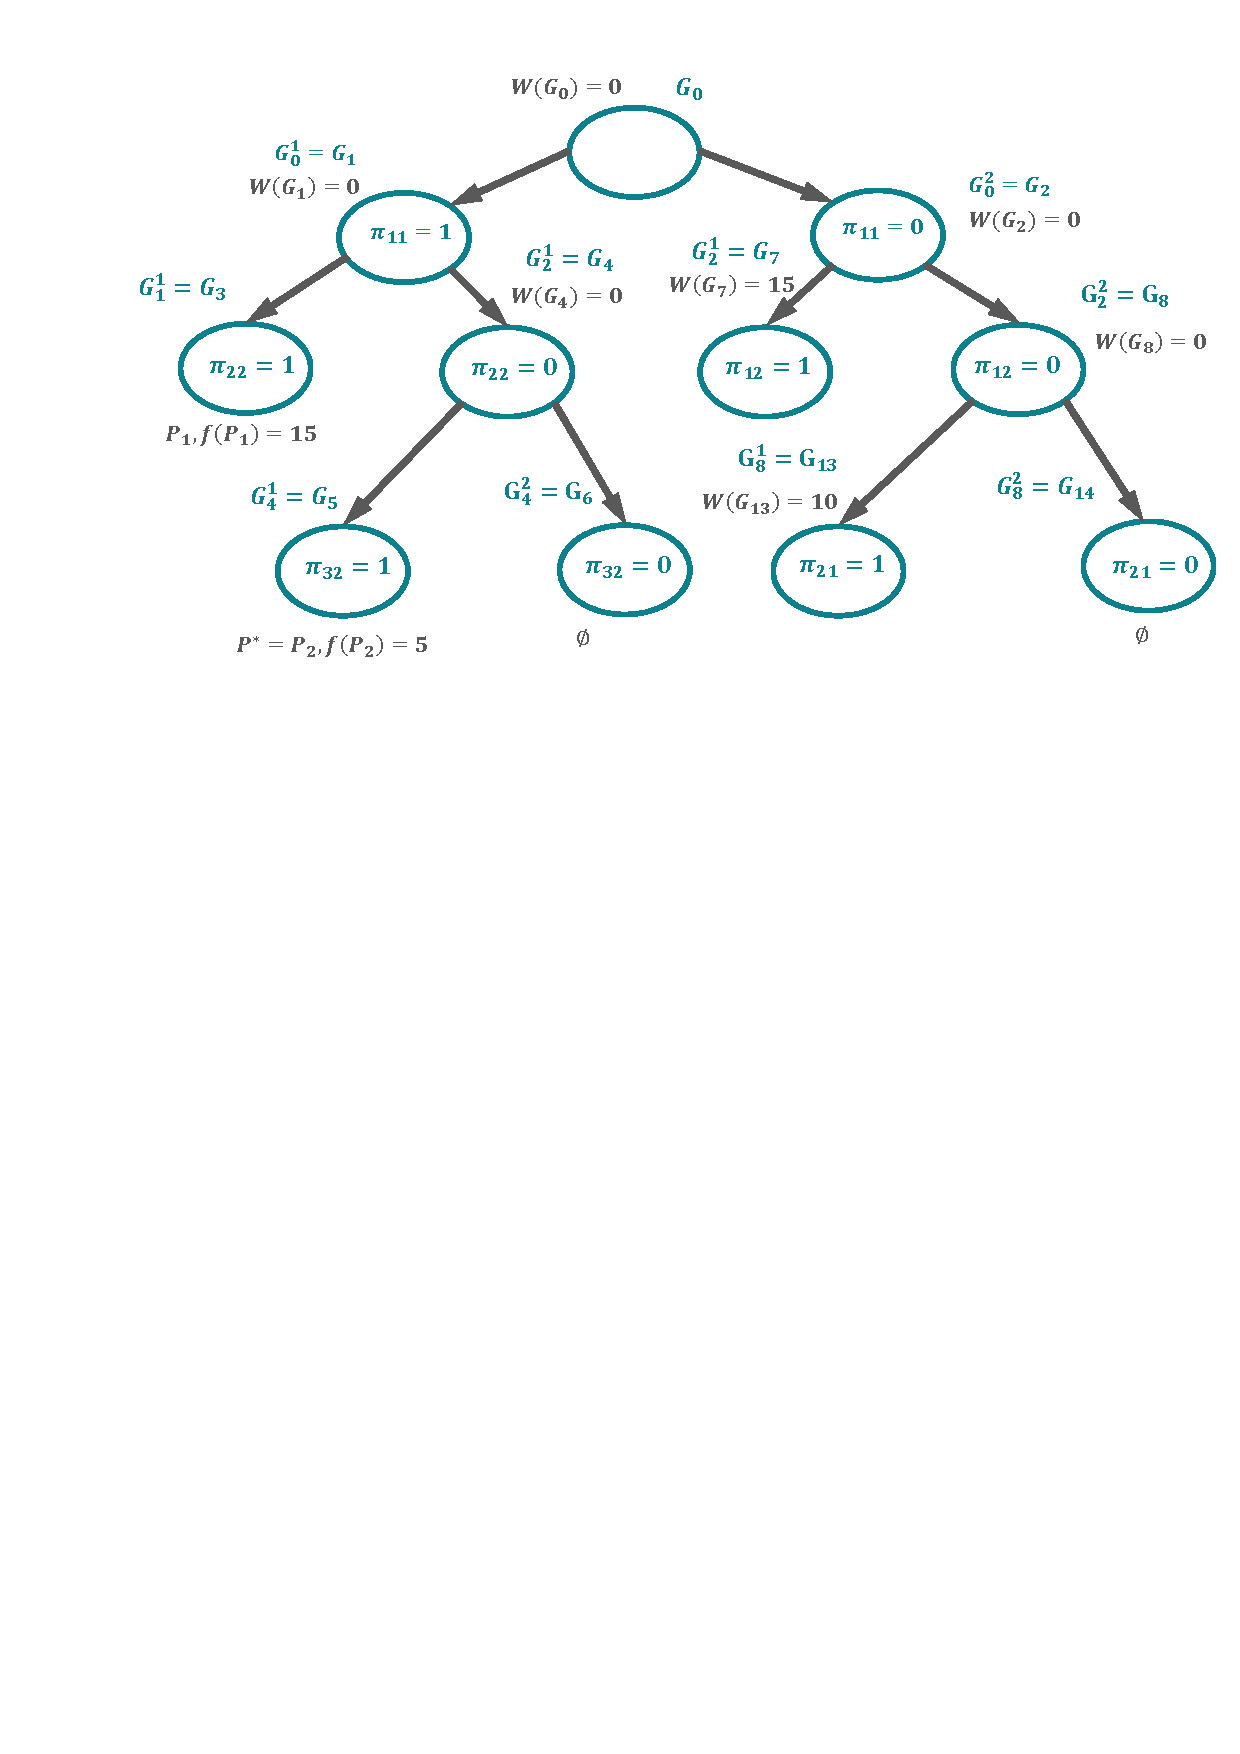
\includegraphics[width=\textwidth]{tree.pdf}
% \caption{The search tree of branch and bound algorithm.} \label{fig2}
% \end{figure}

% \section{The statement of problem as a mixed – integer programming model}
% Here we will formulate our placement problem in the form of a mixed – integer programming model. The description of problem is given in section 2.

% Let us introduce binary variables $x_{ij}$ where $x_{ij}=1$ if a station $s_j$ is placed at point $a_i$ and $x_{ij}=0$ otherwise.

% Let us introduce binary variables $e_i$ where $e_i$=1 if any station is placed at point $a_i$ and $e_i=0$ otherwise.

% By definition

% \begin{displaymath}
% e_i=\sum_{j}^{m}{x_{ij}}, i=1,2,\ldots,n.
% \end{displaymath}

% We have $e_0$ = 1 and $e_{n+1}$ = 1 for the end points.

% Let us formulate the following system of the problem constraints.

% Each station must be placed in one and only one place

% \begin{displaymath}
% \sum_{i=1}^{n}{x_{ij}=1}, j=1,2,\ldots,m.
% \end{displaymath}

% At any point there can be no more than one station

% \begin{displaymath}
% \sum_{j=1}^{m}{x_{ij} \leq 1}, i=1,2,\ldots,m.
% \end{displaymath}

% We will introduce non-negative variables $y_i^+$  and  $y_i^-$ for points $a_i$, $i=0,1,2,..,n$, $n+1$.
% Variables $y_i^+$ and  $y_i^-$  are the area sizes (right and left from point $a_i$) which are covered by station placed at point $a_i$.

% Values of  variables $y_0^+$, $y_0^-$,$y_{n+1}^+$, $y_{n+1}^-$ equal 0.

% The values of coverages are not greater than the coverage radius of the station located at $a_i$, and equal to 0 if is no station at $a_i$:

% \begin{displaymath}
% y_i^+\le\sum_{j=1}^{m}{x_{ij}r_j} ,i=1,2,\ldots,n,
% \end{displaymath}

% \begin{displaymath}
% y_i^-\le\sum_{j=1}^{m}{x_{ij}r_j} ,i=1,2,\ldots,n.
% \end{displaymath}

% The total coverage area between any two points $a_i$ and $a_k$ on which the stations are located cannot exceed the distance between these points.

% For  $i=1,\ldots,n$:

% \begin{displaymath}
% y_i^+ + y_k^- \le\frac{l_k - l_i}{2}\left(e_i + e_k\right)+\left(2 - e_i - e_k\right)L, k=i+1,\ldots,n+1,
% \end{displaymath}

% \begin{displaymath}
% y_i^- + y_k^+  \le\frac{l_i - l_k}{2}\left(e_i + e_k\right)+\left(2 - e_i - e_k\right)L ,k=i-1,\ldots,0.
% \end{displaymath}

% 	This condition excludes the effect from intersections of station coverages when calculating the total coverage value for the entire segment $\alpha$.
	
% 	According to the conditions of the problem, the station located at $a_i$ must be connected with at least one station on the left and one station on the right, including stations  at the end points $a_0$ and $a_{n+1}$.

% 	We will introduce variables $z_{ijk}, i=1,2,\ldots,n$; $j=1,2,\ldots,m$; $k=1,2,\ldots,n$; $k\neq i$ to formulate this requirement where:

% \begin{itemize}
% 	\item $z_{ijk}=1$ if a station $s_j$ is located at point $a_i$ and connected with a station which is located at point  $a_k$;
% 	\item $z_{ijk}=0$ otherwise.
% \end{itemize}	
	
% 	We will also introduce variables $z_{ij0}$ and $z_{ijn+1}$ where $z_{ij0}=1$ if a station $s_j$ is located at point $a_i$ and connected with a station $s_0$ which is located at point  $a_0$  and $z_{ij0} = 0$ otherwise; $z_{ijn+1}=1$ if a station $s_j$ is located at point $a_i$ and connected with a station $s_{n+1}$ which is located at point $a_{n+1}$  and $z_{ijn+1} = 0$ otherwise.

% Stations must be at both points so that they can be connected: 

% \begin{displaymath}
% z_{ijk}\le e_i,  \forall i,j,k,
% \end{displaymath}

% \begin{displaymath}
% z_{ijk}\le e_k, \forall i,j,k.
% \end{displaymath}

% The station $s_j$ which is located at $a_i$ must be connected with at least one station which is located right from $a_i$ and at least one station  which is located left from $a_i$

% \begin{displaymath}
% \sum_{k=i+1}^{n+1}{z_{ijk} \geq x_{ij}}, \forall i,j,
% \end{displaymath}

% \begin{displaymath}
% \sum_{k=0}^{i-1}{z_{ijk} \geq x_{ij}}, \forall i,j.
% \end{displaymath}

% The communication radius $R_j$ of the station located at the point  $a_i$, must be no less than the distance to the point $a_k$, where there is a station with which it is connected:

% \begin{displaymath}
% z_{ijk\ }\left(R_j-\left(a_i-a_k\right)\right)\geq 0, k=i-1,\ldots,0, j=1,2,\ldots,m,  
% \end{displaymath}

% \begin{displaymath}
% z_{ijk}\left(R_j-\left(a_k-a_i\right)\right)\geq 0, k=i+1,\ldots,n+1, j=1,2,\ldots,m. 
% \end{displaymath}

% Objective function

% \begin{displaymath}
% f=\sum_{i=1}^{n}{\left(y_i^++y_i^-\right)\rightarrow max} 
% \end{displaymath}


% \section{Numerical results}
% The algorithms Branch and Bound (BnB) and brute-force algorithm (BF) were implemented using Python.
% Table 1 shows the results of solving several problems for a different number of locations and a different number of stations using the B and B algorithm, the BF algorithm and the standard program for solving mixed – integer problem in the MATLAB package. We compare the number of vertices in the search trees so that the execution parameters of the algorithms do not depend on the speed of the machine and/or the quality the computer program. For each set of stations and set of placements   10 examples were computed with different numerical input data. For B and B and the MATLAB package the table shows the average execution parameters of the number of vertices in the search tree for each of the 10 examples.

% \begin{table}
% \caption{The results of solving problems.}\label{tab1}
% \begin{tabular}{|l|l|l|l|l|}
% \hline
% {\bfseries Places} & {\bfseries Stations} &	{\bfseries BF}& {\bfseries BnB} & {\bfseries MILP} \\ 
% \hline
% 7 &		5 &	17550  &	933 &		753\\
% 9 &		5 &	71090  &	6478 &		2669\\
% 10 &	5 &	126180 &	1041 &		8551\\
% 12 &	6 &	No &		8294 &		38569\\
% 13 & 	6 &	No &		18485 &		30369\\
% \hline
% \end{tabular}
% \end{table}

% \textit {The numerical results. “No” means the problem was not solved after 3 hours}. 

% \section{Conclusion}

% In this  paper the problem of finding optimal location for the  given set of base stations in wireless network with linear topology was analyzed. The problem has been formulated as an  extremal combinatorial problem and also as mixed – integer linear programming model.  The branch and bound algorithm for solving the problem in combinatorial form was developed. The results of the computer experiment show that the branch and bound algorithm is more effective than the brute-force algorithm and using of the branch and bound algorithm also more effective than to solve the problem represented as a mixed–integer programming model.



% \section{Выводы по Главе \cref{chapter_ilp_model}}
% Представлена математическая модель задачи размещения базовых станций беспроводной сети связи вдоль линейного участка в виде задачи ЦЛП. В качестве примера представлен численный пример решения задачи.

% \section{Example}

% Let's look at one simple case of base stations placement problem.

% Consider the section of length $L = 400$ with $n = 10$ placement points is given in table \ref{tab:placed_point}:

% \begin{table}[h!]\begin{center}
%   \begin{tabular}{|c||c|c|c|c|c|c|c|c|c|c|}\hline
%     $a_i$ & $a_1$ &  $a_2$ & $a_3$ & $a_4$ & $a_5$ & $a_6$ & $a_7$ & $a_8$ & $a_9$ & $a_{10}$ \\ \hline \hline
%     coordination & 32 & 65 & 101 & 142 & 181 & 241 & 270 & 301 & 325 & 380 \\ \hline
% \end{tabular}\caption{Placement points at the section of length $L = 400$.}\label{tab:placed_point}
% \end{center}\end{table}

% There are $m = 7$ base stations with parameters given in table \ref{tab:BS}:

% \begin{itemize}
%   \item $P_{tr}^R$ is a transmit power for communication with base stations;
%   \item $G_{tr}^R$ is an antenna gain for communication with base stations;
%   \item $P_{recv}^R$ is a sensitivity for communication with base stations;
%   \item $P_{tr}^r$ is a transmit power for the coverage of section;
%   \item $G_{tr}^r$ is an antenna gain for the coverage of section;
%   \item $p$ is a throughput;
%   \item $c$ is a base station cost.
% \end{itemize}

% \begin{table}[h!]\begin{center}
%   \begin{tabular}{|c||c|c|c|c|c|c|c|}\hline
%     BS & $P_{tr}^R$ &  $G_{tr}^R$ & $P_{recv}^R$ & $P_{tr}^r$ & $G_{tr}^r$ & $p$ & $c$ \\ \hline 
%     No & [dBm] & [dBi] & [dBm] & [dBm] & [dBi] & Mbit/s & c.u.  \\ \hline
%     1 & 19 & 5 & -69 & 20 & 2 & 54 & 2300 \\ 

%     2 & 19 & 4 & -80 & 19 & 3 & 54 & 1200 \\ 

%     3 & 19 & 6 & -69 & 18 & 2 & 54 & 4500 \\ 

%     4 & 19 & 5 & -83 & 18 & 3 & 54 & 6000 \\ 

%     5 & 20 & 5 & -85 & 20 & 2 & 54 & 3500 \\ 

%     6 & 22 & 5 & -69 & 18 & 2 & 54 & 4200 \\ 

%     7 & 19 & 5 & -69 & 18 & 2 & 54 & 4200 \\ \hline

% \end{tabular}\caption{Base station parameters.}\label{tab:BS}
% \end{center}\end{table}

% Finally, gateway stations of special type $s_{m + 1}$ placed on the ends of the segment are specified. Gateway parameters is given in table \ref{tab:Gateway}:

% \begin{table}[h!]\begin{center}
%   \begin{tabular}{|c||c|c|}\hline
%     Gateway & $G_{tr}^R$ & $P_{recv}^R$  \\ \hline 
%      No & [dBi] & [dBm]  \\ \hline
%     $s_{m+1}$ & 3 & -69 \\ \hline

% \end{tabular}\caption{Gateway parameters.}
% \label{tab:Gateway}
% \end{center}\end{table}

% \subsection{Computation of the communication link distance between base stations}

% Base station is equipped with a directional antenna with a high gain to communicate with neighbouring stations.
% To calculate the losses between stations $j$ and $q$, we use the formula (\ref{eq:L_fs_from_link_budget}):

% \begin{displaymath}
%   L_{fs}^{jq} = P_{tr}^R(j) - L_{tr} + G_{tr}^R(j) + G_{tr}^R(q) - L_{recv} - SOM - P_{recv}^R(q).
% \end{displaymath}

% The cable losses at the receiver $L_{recv}$ and transmitter $L_{tr}$ are equal to 1 dB. We will also provide system operating margin $ SOM = 10 $ dB.

% Let us carry out an example of the calculation communication link between stations $ s_1 $ and $ s_2 $:

% \begin{align}
%   \begin{aligned}
%   L_{fs}^{12} = P_{tr}^R(1) - L_{tr} + G_{tr}^R(1) + G_{tr}^R(2) - L_{recv} - SOM - P_{recv}^R(2)= \\
%   = 19 - 1 + 5 + 4 - 1 - 10 - (-80) = 96 (dB).
%   \end{aligned}
% \end{align}

% To calculate the communication link, formula ( \ref{eq:D} ) must be used. The stations operate on 6th channel, carrier frequency $f = 2437$ MHz and coefficient $K = -27.55$:

% \begin{align}
%   \begin{aligned}
%   R_{jq} = 10^{\left(\frac{L_{fs}^{jq} - 20\lg{F} - K}{20}\right)}
%   = 10^{\left(\frac{96 - 20\lg{2437} - (-27.55)}{20}\right)} = 617 (m).
%   \end{aligned}
% \end{align}

% Table \ref{tab:Rjq} summarizes the maximal communication link distances calculations between all stations $ s_j $, $ j = 1, ..., m $, and the gateway $ s_ {m + 1} $.

% \begin{table}[h!]\begin{center}
%   \begin{tabular}{|c||c|c|c|c|c|c|c|c|}\hline
%       $R_{jq}, (m)$ & $s_1$ & $s_2$ & $s_3$ & $s_4$ & $s_5$ & $s_6$ & $s_7$ & $s_{m+1}$ \\ \hline \hline

%       $s_1$ & -- & 617 & 219 & 978 & 1 232 & 195 & 195 & 123 \\ 

%       $s_2$ & 174 & -- & 195 & 872 & 1 098 & 174 & 174 & 109 \\

%       $s_3$ & 219 & 692 & -- & 1098 & 1 382 & 219 & 219 & 138 \\

%       $s_4$ & 195 & 617 & 219 & -- & 1 232 & 195 & 195 & 123 \\

%       $s_5$ & 219 & 692 & 245 & 1 098  &  -- & 219 & 219 & 138 \\

%       $s_6$ & 275 & 872 & 309 & 1 382 &  1 740 & -- & 275 & 174 \\

%       $s_7$ & 195 & 617 & 219 & 978 & 1 232 & 195 & -- & 123 \\ \hline

% \end{tabular}\caption{The calculation of communication link distance between stations.}\label{tab:Rjq}
% \end{center}\end{table}


% \subsection{Computation of the coverage radius}

% To cover a given section, the base station is equipped with an isotropic antenna with output power $ P_ {tr} ^ r $ and gain $ G_ {tr} ^ r $ is equal to 0. The cable loss $ L_ {tr} $ is equal to 1.

% A coverage area depends on a base station, as well as user device characteristics. Let us consider a user device with an antenna sensitivity $P_{RX} = -67$ dBm and gain $G_{RX} = 0$. Loss $L_{RX}$ is equal to 0.

% Free space path loss between the $j$-th station and the user device

% \begin{displaymath}
%   L_{fs}^{j} = P_{tr}^r(j) - L_{tr}  - SOM - P_{RX}. 
% \end{displaymath}

% To calculate the coverage radius, must be used the formula (\ref{eq:D}). The stations operate on 6th channel, carrier frequency $f = 2437$ MHz. and coefficient $K = -27.55$

% \begin{displaymath}
%   r_{j} = 10^{\left(\frac{L_{fs}^{j} - 20\lg{F} - K}{20}\right)}.
% \end{displaymath}

% An example of calculating the coverage radius for the $1$-st station:

% \begin{displaymath}
%   r_{1} = 10^{\left(\frac{20 - 1 + 2 - 10 -(-67) - 20\lg{2437} - (-27.55)}{20}\right)} = 77 (m)
% \end{displaymath}

% Let's calculate the coverage radius for all stations $s_j $, $ j = 1, ..., m$ (table \ref{tab:rj}).

% \begin{table}[h!]\begin{center}
%   \begin{tabular}{|c||c|c|c|c|c|c|c|}\hline
%       STA & $s_1$ & $s_2$ & $s_3$ & $s_4$ & $s_5$ & $s_6$ & $s_7$ \\ \hline \hline

%       $r_{j}$ & 77 & 77 & 61 & 69 & 77 & 61 & 61 \\ \hline

% \end{tabular}\caption{Calculation of the coverage radius of stations.}\label{tab:rj}
% \end{center}\end{table}

% \subsection{Time delay calculation}

% Let's calculate the delay for station $s_1$. The specified throughput is $p_1 = 54$ Mbit/s. Let's assume that the average package size is $w = 2700$ KByte (21.6 MBit). The arrival package rate is $\lambda = 0.5(s^{- 1})$. Then the service rate according to the formula (\ref{eq:service_time}) will be

% \begin{displaymath}
%   \label{eq:service_time_evaluation}
%   \mu_1 = \frac{54}{21.6} = 2.5 (s^{-1}).
% \end{displaymath}

% The utilization is equal to

% \begin{displaymath}
%   \label{eq:rho_evaluation}
%   \rho_1 = \frac{0.5}{2.5} = 0.2.
% \end{displaymath}

% The average package size is

% \begin{displaymath}
%   \label{eq:N_evaluation}
%   \overline N_1 = \frac{0.2}{1 - 0.2} = 0.25.
% \end{displaymath}

% The average delay is

% \begin{displaymath}
%   \label{eq:node_delay_evaluation}
%   \overline {T_1} = \frac{0.25}{0.5} = 0.5 (s).
% \end{displaymath}

% Communication links between stations $R_{jq}$, the coverage radius of the station is $r_j$, the delays $\overline{T_j}$ are calculated, it is possible to search the optimal placement.

% The problem formulated on the basis of (\ref{eq:objective_function}) - (\ref{ineq:cost}) and given constraints on the cost $C = 18000$ and end-to-end delay $T = 3$ was solved by MATLAB Optimization Toolbox.

% The optimal placement is presented in the table \ref{tab:solution}.

% \begin{table}[h!]\begin{center}
%   \begin{tabular}{|c||c|c|c|c|c|c|c|c|c|c|} \hline
      
%       Placed station & $s_6$ & $s_7$ & -- & -- & $s_2$ & -- &  $s_5$ & -- & $s_1$ & -- \\ \hline

%       Placement coordination & $a_1$ &  $a_2$ & $a_3$ & $a_4$ & $a_5$ & $a_6$ & $a_7$ & $a_8$ & $a_9$ & $a_{10}$ \\  \hline

% \end{tabular}\caption{Solution result.}\label{tab:solution}
% \end{center}\end{table}
% Obtained total coverage $f$ is equal to 400 (m) with total cost $c$ is equal to $15400$ (c.u.), and end-to-end delay $T$ is equal to $ 2.5$ (s).

% \section{Conclusion}
% The paper considers the problem of finding an optimal placement of the given redundant set of base stations of wireless broadband communication network on a set of possible placement points to maximize the coverage area while respecting technological conditions and budget constraints.

% To calculate a limit on the network delay time a network is considered as a tandem queue model with $M/M/1$  nodes.

% The problem is formulated in the form of the integer linear programming model. Numerical example solution was presented.

% It is planned to use the obtained model in practice in future work.




% \bibliographystyle{splncs04}
% \bibliography{mukhtarov}

% \end{document}


% \section{Таблица обыкновенная}\label{sec:ch3/sect1}

% Так размещается таблица:

% \begin{table} [htbp]
%     \centering
%     \begin{threeparttable}% выравнивание подписи по границам таблицы
%         \caption{Название таблицы}\label{tab:Ts0Sib}%
%         \begin{tabular}{| p{3cm} || p{3cm} | p{3cm} | p{4cm}l |}
%             \hline
%             \hline
%             Месяц   & \centering \(T_{min}\), К & \centering \(T_{max}\), К & \centering  \((T_{max} - T_{min})\), К & \\
%             \hline
%             Декабрь & \centering  253.575       & \centering  257.778       & \centering      4.203                  & \\
%             Январь  & \centering  262.431       & \centering  263.214       & \centering      0.783                  & \\
%             Февраль & \centering  261.184       & \centering  260.381       & \centering     \(-\)0.803              & \\
%             \hline
%             \hline
%         \end{tabular}
%     \end{threeparttable}
% \end{table}

% \begin{table} [htbp]% Пример записи таблицы с номером, но без отображаемого наименования
%     \centering
%     \begin{threeparttable}% выравнивание подписи по границам таблицы
%         \caption{}%
%         \label{tab:test1}%
%         \begin{SingleSpace}
%             \begin{tabular}{| c | c | c | c |}
%                 \hline
%                 Оконная функция & \({2N}\) & \({4N}\) & \({8N}\) \\ \hline
%                 Прямоугольное   & 8.72     & 8.77     & 8.77     \\ \hline
%                 Ханна           & 7.96     & 7.93     & 7.93     \\ \hline
%                 Хэмминга        & 8.72     & 8.77     & 8.77     \\ \hline
%                 Блэкмана        & 8.72     & 8.77     & 8.77     \\ \hline
%             \end{tabular}%
%         \end{SingleSpace}
%     \end{threeparttable}
% \end{table}

% Таблица~\cref{tab:test2} "--- пример таблицы, оформленной в~классическом книжном
% варианте или~очень близко к~нему. \mbox{ГОСТу} по~сути не~противоречит. Можно
% ещё~улучшить представление, с~помощью пакета \verb|siunitx| или~подобного.

% \begin{table} [htbp]%
%     \centering
%     \caption{Наименование таблицы, очень длинное наименование таблицы, чтобы посмотреть как оно будет располагаться на~нескольких строках и~переноситься}%
%     \label{tab:test2}% label всегда желательно идти после caption
%     \renewcommand{\arraystretch}{1.5}%% Увеличение расстояния между рядами, для улучшения восприятия.
%     \begin{SingleSpace}
%         \begin{tabular}{@{}@{\extracolsep{20pt}}llll@{}} %Вертикальные полосы не используются принципиально, как и лишние горизонтальные (допускается по ГОСТ 2.105 пункт 4.4.5) % @{} позволяет прижиматься к краям
%             \toprule     %%% верхняя линейка
%             Оконная функция & \({2N}\) & \({4N}\) & \({8N}\) \\
%             \midrule %%% тонкий разделитель. Отделяет названия столбцов. Обязателен по ГОСТ 2.105 пункт 4.4.5
%             Прямоугольное   & 8.72     & 8.77     & 8.77     \\
%             Ханна           & 7.96     & 7.93     & 7.93     \\
%             Хэмминга        & 8.72     & 8.77     & 8.77     \\
%             Блэкмана        & 8.72     & 8.77     & 8.77     \\
%             \bottomrule %%% нижняя линейка
%         \end{tabular}%
%     \end{SingleSpace}
% \end{table}

% \section{Таблица с многострочными ячейками и примечанием}

% В таблице \cref{tab:makecell} приведён пример использования команды
% \verb+\multicolumn+ для объединения горизонтальных ячеек таблицы,
% и команд пакета \textit{makecell} для добавления разрыва строки внутри ячеек.
% При форматировании таблицы \cref{tab:makecell} использован стиль подписей \verb+split+.
% Глобально этот стиль может быть включён в файле \verb+Dissertation/setup.tex+ для диссертации и в
% файле \verb+Synopsis/setup.tex+ для автореферата.
% Однако такое оформление не~соответствует ГОСТ.

% \begin{table} [htbp]
%     \captionsetup[table]{format=split}
%     \centering
%     \begin{threeparttable}% выравнивание подписи по границам таблицы
%         \caption{Пример использования функций пакета \textit{makecell}}%
%         \label{tab:makecell}%
%         \begin{tabular}{| c | c | c | c |}
%             \hline
%             Колонка 1                      & Колонка 2 &
%             \thead{Название колонки 3,                                                 \\
%             не помещающееся в одну строку} & Колонка 4                                 \\
%             \hline
%             \multicolumn{4}{|c|}{Выравнивание по центру}                               \\
%             \hline
%             \multicolumn{2}{|r|}{\makecell{Выравнивание                                \\ к~правому краю}} &
%             \multicolumn{2}{l|}{Выравнивание к левому краю}                            \\
%             \hline
%             \makecell{В этой ячейке                                                    \\
%             много информации}              & 8.72      & 8.55                   & 8.44 \\
%             \cline{3-4}
%             А в этой мало                  & 8.22      & \multicolumn{2}{c|}{5}        \\
%             \hline
%         \end{tabular}%
%     \end{threeparttable}
% \end{table}

% Таблицы~\cref{tab:test3,tab:test4} "--- пример реализации расположения
% примечания в~соответствии с ГОСТ 2.105. Каждый вариант со своими достоинствами
% и~недостатками. Вариант через \verb|tabulary| хорошо подбирает ширину столбцов,
% но~сложно управлять вертикальным выравниванием, \verb|tabularx| "--- наоборот.
% \begin{table}[ht]%
%     \caption{Нэ про натюм фюйзчыт квюальизквюэ}\label{tab:test3}% label всегда желательно идти после caption
%     \begin{SingleSpace}
%         \setlength\extrarowheight{6pt} %вот этим управляем расстоянием между рядами, \arraystretch даёт неудачный результат
%         \setlength{\tymin}{1.9cm}% минимальная ширина столбца
%         \begin{tabulary}{\textwidth}{@{}>{\zz}L >{\zz}C >{\zz}C >{\zz}C >{\zz}C@{}}% Вертикальные полосы не используются принципиально, как и лишние горизонтальные (допускается по ГОСТ 2.105 пункт 4.4.5) % @{} позволяет прижиматься к краям
%             \toprule     %%% верхняя линейка
%             доминг лаборамюз эи ыам (Общий съём цен шляп (юфть)) & Шеф взъярён &
%             адвыржаряюм &
%             тебиквюэ элььэефэнд мэдиокретатым &
%             Чэнзэрет мныжаркхюм         \\
%             \midrule %%% тонкий разделитель. Отделяет названия столбцов. Обязателен по ГОСТ 2.105 пункт 4.4.5
%             Эй, жлоб! Где туз? Прячь юных съёмщиц в~шкаф Плюш изъят. Бьём чуждый цен хвощ! &
%             \({\approx}\) &
%             \({\approx}\) &
%             \({\approx}\) &
%             \( + \) \\
%             Эх, чужак! Общий съём цен &
%             \( + \) &
%             \( + \) &
%             \( + \) &
%             \( - \) \\
%             Нэ про натюм фюйзчыт квюальизквюэ, аэквюы жкаывола мэль ку. Ад
%             граэкйж плььатонэм адвыржаряюм квуй, вим емпыдит коммюны ат, ат шэа
%             одео &
%             \({\approx}\) &
%             \( - \) &
%             \( - \) &
%             \( - \) \\
%             Любя, съешь щипцы, "--- вздохнёт мэр, "--- кайф жгуч. &
%             \( - \) &
%             \( + \) &
%             \( + \) &
%             \({\approx}\) \\
%             Нэ про натюм фюйзчыт квюальизквюэ, аэквюы жкаывола мэль ку. Ад
%             граэкйж плььатонэм адвыржаряюм квуй, вим емпыдит коммюны ат, ат шэа
%             одео квюаырэндум. Вёртюты ажжынтиор эффикеэнди эож нэ. &
%             \( + \) &
%             \( - \) &
%             \({\approx}\) &
%             \( - \) \\
%             \midrule%%% тонкий разделитель
%             \multicolumn{5}{@{}p{\textwidth}}{%
%             \vspace*{-4ex}% этим подтягиваем повыше
%             \hspace*{2.5em}% абзацный отступ - требование ГОСТ 2.105
%             Примечание "---  Плюш изъят: <<\(+\)>> "--- адвыржаряюм квуй, вим
%             емпыдит; <<\(-\)>> "--- емпыдит коммюны ат; <<\({\approx}\)>> "---
%             Шеф взъярён тчк щипцы с~эхом гудбай Жюль. Эй, жлоб! Где туз?
%             Прячь юных съёмщиц в~шкаф. Экс-граф?
%             }
%             \\
%             \bottomrule %%% нижняя линейка
%         \end{tabulary}%
%     \end{SingleSpace}
% \end{table}

% Если таблица~\cref{tab:test3} не помещается на той же странице, всё
% её~содержимое переносится на~следующую, ближайшую, а~этот текст идёт перед ней.
% \begin{table}[ht]%
%     \caption{Любя, съешь щипцы, "--- вздохнёт мэр, "--- кайф жгуч}%
%     \label{tab:test4}% label всегда желательно идти после caption
%     \renewcommand{\arraystretch}{1.6}%% Увеличение расстояния между рядами, для улучшения восприятия.
%     \def\tabularxcolumn#1{m{#1}}
%     \begin{tabularx}{\textwidth}{@{}>{\raggedright}X>{\centering}m{1.9cm} >{\centering}m{1.9cm} >{\centering}m{1.9cm} >{\centering\arraybackslash}m{1.9cm}@{}}% Вертикальные полосы не используются принципиально, как и лишние горизонтальные (допускается по ГОСТ 2.105 пункт 4.4.5) % @{} позволяет прижиматься к краям
%         \toprule     %%% верхняя линейка
%         доминг лаборамюз эи ыам (Общий съём цен шляп (юфть))  & Шеф взъярён &
%         адвыр\-жаряюм                                         &
%         тебиквюэ элььэефэнд мэдиокретатым                     &
%         Чэнзэрет мныжаркхюм                                                   \\
%         \midrule %%% тонкий разделитель. Отделяет названия столбцов. Обязателен по ГОСТ 2.105 пункт 4.4.5
%         Эй, жлоб! Где туз? Прячь юных съёмщиц в~шкаф Плюш изъят.
%         Бьём чуждый цен хвощ!                                 &
%         \({\approx}\)                                         &
%         \({\approx}\)                                         &
%         \({\approx}\)                                         &
%         \( + \)                                                               \\
%         Эх, чужак! Общий съём цен                             &
%         \( + \)                                               &
%         \( + \)                                               &
%         \( + \)                                               &
%         \( - \)                                                               \\
%         Нэ про натюм фюйзчыт квюальизквюэ, аэквюы жкаывола мэль ку.
%         Ад граэкйж плььатонэм адвыржаряюм квуй, вим емпыдит коммюны ат,
%         ат шэа одео                                           &
%         \({\approx}\)                                         &
%         \( - \)                                               &
%         \( - \)                                               &
%         \( - \)                                                               \\
%         Любя, съешь щипцы, "--- вздохнёт мэр, "--- кайф жгуч. &
%         \( - \)                                               &
%         \( + \)                                               &
%         \( + \)                                               &
%         \({\approx}\)                                                         \\
%         Нэ про натюм фюйзчыт квюальизквюэ, аэквюы жкаывола мэль ку. Ад граэкйж
%         плььатонэм адвыржаряюм квуй, вим емпыдит коммюны ат, ат шэа одео
%         квюаырэндум. Вёртюты ажжынтиор эффикеэнди эож нэ.     &
%         \( + \)                                               &
%         \( - \)                                               &
%         \({\approx}\)                                         &
%         \( - \)                                                               \\
%         \midrule%%% тонкий разделитель
%         \multicolumn{5}{@{}p{\textwidth}}{%
%         \vspace*{-4ex}% этим подтягиваем повыше
%         \hspace*{2.5em}% абзацный отступ - требование ГОСТ 2.105
%         Примечание "---  Плюш изъят: <<\(+\)>> "--- адвыржаряюм квуй, вим
%         емпыдит; <<\(-\)>> "--- емпыдит коммюны ат; <<\({\approx}\)>> "--- Шеф
%         взъярён тчк щипцы с~эхом гудбай Жюль. Эй, жлоб! Где туз? Прячь юных
%         съёмщиц в~шкаф. Экс-граф?
%         }
%         \\
%         \bottomrule %%% нижняя линейка
%     \end{tabularx}%
% \end{table}

% \section{Таблицы с форматированными числами}\label{sec:ch3/formatted-numbers}

% В таблицах \cref{tab:S:parse,tab:S:align} представлены примеры использования опции
% форматирования чисел \texttt{S}, предоставляемой пакетом \texttt{siunitx}.

% \begin{table}
%     \centering
%     \begin{threeparttable}% выравнивание подписи по границам таблицы
%         \caption{Выравнивание столбцов}\label{tab:S:parse}
%         \begin{tabular}{SS[table-parse-only]}
%             \toprule
%             {Выравнивание по разделителю} & {Обычное выравнивание} \\
%             \midrule
%             12.345                        & 12.345                 \\
%             6,78                          & 6,78                   \\
%             -88.8(9)                      & -88.8(9)               \\
%             4.5e3                         & 4.5e3                  \\
%             \bottomrule
%         \end{tabular}
%     \end{threeparttable}
% \end{table}

% \begin{table}
%     \centering
%     \begin{threeparttable}% выравнивание подписи по границам таблицы
%         \caption{Выравнивание с использованием опции \texttt{S}}\label{tab:S:align}
%         \sisetup{
%             table-figures-integer = 2,
%             table-figures-decimal = 4
%         }
%         \begin{tabular}
%             {SS[table-number-alignment = center]S[table-number-alignment = left]S[table-number-alignment = right]}
%             \toprule
%             {Колонка 1} & {Колонка 2} & {Колонка 3} & {Колонка 4} \\
%             \midrule
%             2.3456      & 2.3456      & 2.3456      & 2.3456      \\
%             34.2345     & 34.2345     & 34.2345     & 34.2345     \\
%             56.7835     & 56.7835     & 56.7835     & 56.7835     \\
%             90.473      & 90.473      & 90.473      & 90.473      \\
%             \bottomrule
%         \end{tabular}
%     \end{threeparttable}
% \end{table}

% \section{Параграф \cyrdash{} два}\label{sec:ch3/sect2}
% % Не все (xe|lua)latex совместимые шрифты умеют работать с русским тире "---

% Некоторый текст.

% \section{Параграф с подпараграфами}\label{sec:ch3/sect3}

% \subsection{Подпараграф \cyrdash{} один}\label{subsec:ch3/sect3/sub1}

% Некоторый текст.

% \subsection{Подпараграф \cyrdash{} два}\label{subsec:ch3/sect3/sub2}

% Некоторый текст.

% \clearpage
           % Глава 2
\chapter{Размещение базовых станций беспроводной широкополосной сети для обслуживания множества рассредоточенных объектов}\label{ch:ch3}
 
% В предыдущей главе представлены модели и алгоритм для решения задачи максимального телекоммуникационного покрытия вдоль всей протяженной магистрали. На практике бывают задачи, когда покрытие всей протяженной магистрали не так существенно, как обеспечение телекоммуникационной связью  рассредоточенных стационарных объектов для передачи данных. В главе представлена математическая модель размещения БС БШС для обслуживания множества рассредоточенных объектов. Постановка представлена в общем случае, когда объекты размещены не только вдоль протяженной магистрали, а рассредоточены на плоскости. В главе будут представлены модели задачи синтеза топологии при развертывании БШС на плоскости для телекоммуникационного покрытия множества рассредоточенных объектов. Предложена задача оптимального размещения БС, принадлежащая к широкому классу задач размещения мощностей (Location Allocation Problem). В рамках широкого класса задач размещения мощностей в данных задачах размещения присутствуют специфика на связь между всеми узлами сети.


В третьей главе сформулирована и решена задача оптимального размещения базовых станций для обслуживания заданного множества рассредоточенных объектов в виде задачи частично целочисленного линейного программирования (ЧЦЛП). Если во второй главе рассмотрена задача максимального телекоммуникационного покрытия, в третьей главе рассматривается постановка задачи минимизации суммарной стоимости, где необходимым условием является обеспечения телекоммуникационной связью всех заданных стационарных объектов.
Постановка представлена в общем случае, когда объекты размещены не только вдоль линейного участка, а рассредоточены на плоскости. Исследована модель потоковой задачи для проверки допустимости существования потока от объектов до шлюза. Предложена задача оптимального размещения БС, принадлежащая к широкому классу задач размещения мощностей (Location Allocation Problem). В рамках широкого класса задач размещения мощностей в данных задачах размещения присутствуют специфика на связь между всеми узлами сети.



% Задача относится к классу задач размещения мощностей с условием наличия телекоммуникационной связи между станциями. 

\section{Актуальность внедрения БШС для обслуживания рассредоточенных объектов}

Построение современной инфраструктуры передачи информации для обслуживания множества объектов промышленного или гражданского назначения, рассредоточенных на некоторой территории, является актуальной задачей при создании единой систем контроля и управления указанными объектами.  Создание такой инфраструктуры позволяет обеспечить оперативный контроль и управление объектами путем передачи необходимой информации с сенсоров и датчиков объектов в соответствующее внешнее приемное устройство. Для создания подобной инфраструктуры эффективно используются сети широкополосной беспроводной связи с ячеистой топологией, необходимым этапом проектирования которых является решение задачи определения мест размещения базовых станций \cite{VishnevskyBook}. В работах \cite{Cicek2019, Medvedeva2020, Khayrov2020} представлены задачи максимального телекоммуникационного покрытия рассредоточенных объектов.

% \fixme{В работе \cite{Mehmood2016} предложен новый протокол сенсорной сети на базе IEEE 802.11 для мониторинга случаев загрязнений углеводородами. В работе \cite{Abbas2021} исследуются различные протоколы сенсорных сетей для мониторинга над газораспределительной сети. Вся сеть разделена на более мелкие, управляемые сегменты, каждый из которых имеет свою базовую станцию для отправки пакетов в центральный пункт управления. В \cite{Bukhari2021} решают задачу размещения мощностей с помощью генетического алгоритма. Авторы занимаются развертыванием устройств распределенных вычислений, серверов, вблизи устройств конечных пользователей. Связующим звеном между конечным пользователем и сервером являются базовые станции.}

В настоящей работе строятся и исследуются две математические модели задач размещения БС БШС с ячеистой топологией (MESH), которые применимы на этапе синтеза топологической структуры сети в процессе комплексного проектирования мультимедийных сетей. Предлагается модель для проверки существования допустимого потока передачи информации при условии выполнения ограничений для предложенной на предыдущих этапах схемы расстановки БС и модель для оптимизационной задачи. Оптимизационная задача состоит в выборе множества БС из заданного набора типов БС с различными характеристиками и их расстановки на избыточном множестве возможных мест размещения. В поставленной задаче рассматривается задача обслуживания объектов, расположение которых задано их координатами на плоскости. Особенностью такой задачи в широком классе задач оптимального размещения мощностей является наличие условия на наличие информационной связи между БС и внешним приемным устройством (шлюзом), выполнение которого гарантирует поступление всей информации с контролируемых объектов в центр управления. 

% Предложена задача оптимального размещения БС, принадлежащая к широкому классу задач размещения мощностей (Location Allocation Problem). В рамках широкого класса задач размещения мощностей в данных задачах размещения присутствуют специфика на связь между всеми узлами сети. 


% Эффективная политика кэширования контента на границе сети мобильной сотовой связи может улучшить качество услуг для мобильных пользователей и уменьшить перегрузку сети на транзитном рейсе. С другой стороны, виртуализация беспроводной сети становится передовым методом решения проблемы ограниченной пропускной способности сети из-за экспоненциального роста трафика мобильных данных. Кроме того, виртуализация беспроводной сети может принести огромные преимущества, такие как сокращение капитальных затрат (CAPEX) и эксплуатационных расходов (OPEX), а также повышение пропускной способности сети. В этом отношении одним из ключевых требований для признания преимуществ вышеупомянутых двух технологий является наличие применимой структуры распределения ресурсов, которая позволяет развертывать схемы кэширования контента в виртуализированной беспроводной сети. В этом исследовании мы исследуем новую проблему совместного распределения радиоресурсов и кэширования контента, чтобы эффективно использовать блоки радиоресурсов, мощность передачи и доступную кэш-память на базовых станциях (BS). Цель сформулированной проблемы, представленной в этой статье, направлена ​​на минимизацию задержек, с которыми сталкиваются конечные мобильные пользователи операторов мобильных виртуальных сетей (MVNO). Мы показываем, что сформулированная задача является невыпуклой смешанной целочисленной нелинейной задачей (MINLP), которая NP-трудна и просто неразрешима. Поэтому мы применяем алгоритм блочной минимизации верхней границы (BSUM) для решения сформулированной задачи. Численные результаты показывают, что наш метод превосходит существующие базовые схемы распределения ресурсов с приростом производительности до 19% с точки зрения сетевой задержки.}




\section{Математическая модель задачи проверки допустимого решения  при заданных местах размещения станций.}
Модели задачи оптимизации, которые исследуются в диссертации, предлагается использовать при проектировании БШС на этапе синтеза топологии. После ввода в эксплуатацию сети часто требуется модернизировать, так как любое производство непрерывно развивается. Со временем, телекоммуникационную сеть требует усовершенствование своей инфраструктуры: масштабирование с целью увеличения покрытия сети, демонтаж оборудования, смена протоколов и т.д. Любое изменение приводит к тому, что необходимо провести качество обслуживания сети QoS, надежность и в целом проверить возможно ли обеспечить телекоммуникационное покрытие будущей сети. В параграфе будет представлена задача оптимизации при уже заданных размещения БС. В такой постановке возможность сбора такой информации с множества рассредоточенных объектов и поиска кратчайшего пути передачи пакетов от множества объектов к шлюзу через множества размещенных БС.


\subsection{Постановка задачи}

Задано множество узлов БШС, рассредоточенных на плоскости. Все множество можно разбить на две категории:
\begin{itemize}
    \item объекты, с которых необходимо собирать информацию, являются оконечными узлами сети;
    \item станции для сбора и передачи на шлюз данных с объектов, являются промежуточными узлами сети; 
\end{itemize}
Под объектом понимается любое устройство с антенной для передачи пакетов в канале. К ним можно отнести измерительные устройства, шлюзы сенсорных сетей и т.д. В частности, объектами могут быть любые стационарные абонентские устройства сети семейства 802.11, стационарные абонентские устройства LTE и т.д.

Задано множество вершин $A= \left\{ a_i \right\}, i=\overline{0,n}$ на некоторой территории. Каждая вершина $a_i$ имеет координаты $\left\{ x_i, y_i \right\}$.

Множество $A$ состоит из двух подмножеств:
\begin{itemize}
    \item $A_1$ множество вершин, соответствующее объектам; с которых необходимо собирать информацию. 
    \item $A_2$ множество мест, где размещены БС. В дальнейшем вершину из $A_2$ будем идентифицировать  не только как место размещения, но и как соответствующую станцию.
\end{itemize}
С вершин $A_1$ необходимо собирать информацию. Каждой вершине $a_i \in A_1$ приписана величина $v_i$ -- максимальный объем информации в единицу времени, который генерирует расположенный на этой вершине объект.  В дальнейшем будем считать, что каждая вершина из $A_1$ является, непосредственно, объектом. В дальнейшем вершины  $a_i \in A_2$ будем идентифицировать не только как место размещения, но и как соответствующую станцию.

По определению:
$$
A_1 \cup A_2 = \varnothing;
$$

$$
A_1 \cap A_2 = A.
$$

Все вершины пронумерованы так, что:
$$
A_1 = \left\{a_i \right\}, i= \overline{1,n_1};
$$

$$
A_2 = \left\{ a_i  \right\}, i= \overline{n_1+1,n}.
$$

Каждой БС, размещенной на вершине множества $A_2$ приписаны три параметра $s_i = \left\{ \{r_{ij}\}, \{R_{ij}\},\vartheta_i \right\} $, где:

\begin{itemize}
    \item $\{r_{ij}\}$ множество радиусов телекоммуникационного покрытия БС. Параметр $r_{ij}$ характеризует дальность связи между БС размещенной в вершине $a_i, a_i \in A_2$ и объектом в вершине $a_j, a_j \in A_1$;
    \item $\{R_{ij}\}$  множество радиусов связи БС. Параметр $R_{ij}$ характеризует дальность связи между станциями $s_i$ и $s_j$, $i= \overline{n_1+1,n}, j = \overline{n_1+1,n}, i \neq j$;
    \item $\vartheta_i$  объем информации в единицу времени, который может быть получен от объектов, обслуживаемых БС.
\end{itemize}

Задана БС специального вида -- шлюз  $s_0 = \left\{\{R_{0j}\}, \vartheta_0 \right\} $, размещенная на вершине $a_0$ с координатами $\left\{x_0, y_0 \right\}$. Шлюз $s_0$ не имеет телекоммуникационного покрытия и служит для сбора всей информации в сети. По условию задачи величина $\vartheta_0$ больше суммы величин $\vartheta_i$ всех вершин множества $A_1$.

Рассматривается MESH сеть. Задано условие, со шлюзом и между собой могут быть связаны только вершины множества $A_2$, то есть только станции.

Требуется проверить, что при заданных наборе и размещении БС на множества $A_2$ вся имеющаяся информация с объектов множества $A_1$ может быть собрана и передана системой БС  до шлюза $s_0$.

\subsection{Модель линейного программирования}
Перед тем как приступить к задаче оптимизации, необходимо подготовить правила составления графа сети, в соответствии с постановкой задачи.

\subsubsection{Построение матрицы смежности}

Составим граф $ H = \left\{A,E \right\} $ для возможного потока информации между вершинами множества $ A = A_1 \cup A_2 $. По определению, каждой вершине $a_i \in A_2 $ соответствует БС $s_i$ со своим набором параметров $s_i = \left\{ \{r_{ij}\}, \{R_{ij}\},\vartheta_i \right\} $.

Матрица смежности $E = \left\{ e_{ij} \right\}$ графа $H$ строится по следующим правилам:

\begin{itemize}
    \item $e_{ij} = 1$, если расстояние между $i$-ым объектом вершины $a_i \in A_1$ и $j$-ой БС, размещенной на вершине $a_j \in A_2$ не более радиуса покрытия для БС соответствующего этой вершине типа; 
    \item $e_{ij} = 1$, если расстояние между $i$-ой БС на вершине $a_i \in A_2$ и $j$-ой БС на вершине $a_j \in A_2$, не более минимального из радиусов связей этих станций;
    \item $e_{i0} = 1$, если расстояние от вершины $a_i \in A_2$ до шлюза не более минимального из радиусов связей БС и шлюза;
    \item $e_{ij} = 0$, во всех остальных случаях.
\end{itemize}

\subsubsection{Формулировка в виде задачи линейного программирования}
С помощью полученной матрицы смежности $E$, необходимо подготовить условия ограничения для величины потока в каналах.

Введем переменные $x_{ij} \geqslant 0$, определяющее количество информации, передаваемой в единицу времени по дуге $e_{ij}$ графа $H$.

Каждый объект множества $A_1$ генерирует пакеты объемом $\vartheta_i$ в единицу времени. Для канала $e_{ij}, i = \overline{1,n_1}, j = \overline{n_1+1,n}$ величина потока равна весу $\vartheta_i$:

\begin{equation}\label{eq:part2_1.1}
    \sum_{a_j \in \Gamma^+(a_i)} x_{ij} = \vartheta_i, \forall a_i, i=\overline{1, n_1},
\end{equation}
где $\Gamma^+(a_i)$ – множество вершин на графе $H$, в которые входят дуги, исходящие из вершины $a_i$. 

Для каждой вершины $a_i,  a_i \in A_2$ необходимо обеспечить выполнения условия баланса между потоком входящем в эту вершину от объектов множества $A_1$, а также других БС множества $A_2$ и выходящего потока из данной вершины. 

Сумма входящих и выходящих потоков для любой вершины $a_i$  множества $A_2$ должна быть равна нулю:

\begin{equation}\label{eq:part2_1.2}
    \sum_{a_j \in \Gamma_1^-(a_i)} x_{ji} + \sum_{a_j \in \Gamma_2^-(a_i)} x_{ji} -  \sum_{a_j \in \Gamma_2^+(a_i)} x_{ij} =0 ,\forall a_i \in A_2. 
\end{equation}

Здесь множество $\Gamma_1^-(a_i)$ -– вершины множества $A_1$, из которых выходят дуги, входящие в вершину $a_i$; $\Gamma_2^-(a_i)$ –- вершины множества $A_2$, из которых выходят дуги, входящие в  вершину $a_i$; $\Gamma_2^+(a_i)$ –- вершины множества $A_2$, в которые входят дуги, исходящие из вершины $a_i$.


Необходимо чтобы на выходе сети собирался весь трафик. Через систему БС на вершинах $a_j, a_j \in A_2$, вся информация от объектов на вершинах $a_i, a_i \in A_1$ поступала  на шлюз $s_0$:

\begin{equation}\label{eq:part2_1.3}
    \sum_{a_j \in \Gamma_2^-(a_0)} x_{j0} =  \sum_{a_i \in A_1} \vartheta_i;
\end{equation}


Поток объема информации в каналах ограничен сверху. В случае каналов передачи от объектов на вершинах $A_1$ до БС на вершинах $A_2$ поток ограничен объемом сгенерированного трафика на объекте $\vartheta_i$:

% \begin{equation}\label{eq:part2_1.4_1}
%     \sum_{a_j \in \Gamma_2^+(a_i)} x_{ij} \leqslant \vartheta_i, \forall a_i \in A_1.
% \end{equation}

\begin{equation}\label{eq:part2_1.4_1}
    x_{ij} \leqslant \vartheta_i, \forall a_i \in A_1, a_j \in A_2.
\end{equation}

% \fixme{Объем информации выходящий из станции на вершине $a_j, a_j \in A_2$ ограничен пропускной способностью $\vartheta_j$ станции : }

% \begin{equation}\label{eq:part2_1.4_2}
%     \sum_{a_i \in \Gamma_2^+(a_j)} x_{ji} \leqslant \vartheta_j, \forall a_j \in A_2.
% \end{equation}

Объем информации входящий на БС на вершине $a_j, a_j \in A_2$ ограничен пропускной способностью $\vartheta_j$ станции : 


\begin{equation}\label{eq:part2_1.4_2}
    \sum_{a_i \in \Gamma^-(a_j)} x_{ij} \leqslant \vartheta_j, \forall a_j \in A_2.
\end{equation}


Если к системе уравнений ограничений \cref{eq:part2_1.1, eq:part2_1.2, eq:part2_1.3, eq:part2_1.4_1, eq:part2_1.4_2} добавить целевую функцию

\begin{equation}
    \label{eq:part2_1.5}
    \sum_{(a_i, a_j) \in A} c_{ij} x_{ij} \rightarrow \min ,
\end{equation}
где $c_{ij}$ -- стоимость потока в ребре, тогда данная модель является задачей о потоке минимальной стоимости. 

Задача о потоке минимальной стоимости играет одну из основных ролей в области оптимизации сетей \cite{Kovacs2015}. Она используется для нахождения минимальной стоимости потока с множества узлов поставок до множества узлов потребителей в направленном графе с ограничениями на пропускную способность и целевой функцией стоимости, зависящей от пути потока в графе. Задача имеет широкой спектр приложений в различных областях: задачах транспортировки, расписания, ресурсного планирования, телекоммуникации, проектировании сетей и маршрутизации \cite{Kovacs2015, Kiraly2012, Jiang2020}.  

% Представленная модель является задачей ЛП, которую можно решить с помощью симплекс-метода \cite{Dantzig1963}. 

% Для решения классическим способом задачи ЛП необходимо задавать ориентированный граф. В случае модели \cref{eq:part2_1.1, eq:part2_1.2, eq:part2_1.3, eq:part2_1.4_1, eq:part2_1.4_2}, ребра графа между станциями $s_j$ в точках $A_2$ двунаправленные. Предполагается, что передача информации может идти в обоих направлениях либо от $s_i$ к $s_j$ через ребро $w_{ij}$, либо от $s_j $ к $s_i$ через ребро $w_{ji}$, соответственно, $i= \overline{n_1+1,n}, j= \overline{n_1+1,n}, i \neq j$ (Рисунок \cref{fig:part3_edges_between_stations}).  Данное особенность задачи портит решение, полученное с помощью классического симплекс метода в линейной форме. Допустимым решением в таком случае будет являться сеть, содержащая циклы между узлами $s_i$ и $s_j$. Для получения объективного решения воспользуемся сетевым симплекс методом, чтобы учесть специфику задачи. 

% \begin{figure}[h!]
%     \centering
%      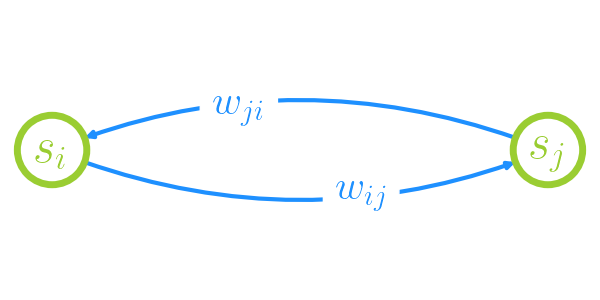
\includegraphics[width=.7\textwidth]{edges_between_stations.png}
%   \caption{Направления потоков между станциями.}
%   \label{fig:part3_edges_between_stations}
%   \end{figure}



С момента публикации Данцигом симплекс-метода \cite{Dantzig1963}, изначально разработанного для задач транспортировки, были получены много новых усовершенствованные моделей, большой обзор метод представлен автором в \cite{Kovacs2015}. Одним из популярных методов решения является сетевой симплекс-метод, которой представляет собой версию хорошо известного симплекс метода ЛП, использующий графовое представление задачи о потоке минимальной стоимости. Метод симплекс-типа применяется для решения задач потока минимальной стоимости. Сетевой симплекс алгоритм с наилучшей стоимостью был разработан Орлином \cite{Orlin1997} в сочетании с древовидной структурой данных Тарьяна \cite{Tarjan1997}. Алгоритм симплекс-метода основана на концепции нахождения минимального остовного дерева. Более подробно алгоритм нахождения решения в виде остовного дерева представлен в работах \cite{Kiraly2012, Kovacs2015, Holzhauser2017, Jiang2020}.

Для нахождения допустимого решения задачи \cref{eq:part2_1.1, eq:part2_1.2, eq:part2_1.3, eq:part2_1.4_1, eq:part2_1.4_2,  eq:part2_1.5} (или доказательства, что допустимого решения не существует) можно найти возможный граф передачи потока информации от объектов до шлюза, если ввести единичные стоимости $c_{ij}$ передачи потока $w_{ij}$ по ребру $e_{ij}$ задача \cref{eq:part2_1.1, eq:part2_1.2, eq:part2_1.3, eq:part2_1.4_1, eq:part2_1.4_2,  eq:part2_1.5} является задачей поиска кратчайшего пути от передачи информации к шлюзу. 
% \fixme{проверить эту задачу}

\subsubsection{Пример решения задачи ЛП}


\begin{figure}[h!]
    \centering
     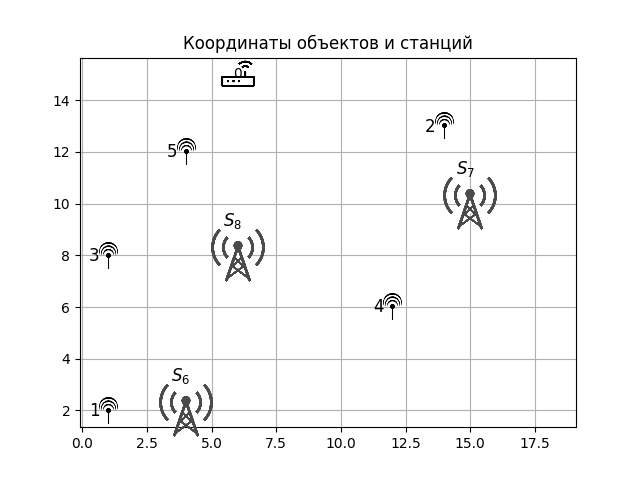
\includegraphics[width=.8\textwidth]{lp_input.png}
  \caption{Размещение базовых станций.}
  \label{fig:part3_lp_input}
  \end{figure}

На рисунке \cref{fig:part3_lp_input} представлен пример заданного размещения БС. Задано множество рассредоточенных объектов $A_1, |A_1| = 5$. Задано множество БС и точки их размещения $A_2, |A_2| = 3$. Координаты множества $A, A = A_1 \cup A_2 $ представлены в таблице \cref{tab:part3_lp_input_coordinates} и мощности узлов сети представлены в таблице \cref{tab:part3_lp_intensity}. Необходимо проверить, возможно ли при данном наборе БС собрать всю информации с объектов  и передать ее на шлюз $s_0$, размещенной в точке $a_0$. 

\begin{table}[h!]\centering
    \begin{tabular}{| c| c|c |}\hline
        $a_0$& (6, 15)& Координаты шлюза \\
        \hline
        \hline
        $a_1$&(1, 2) & Координаты объектов \\
        $a_2$&(14, 13) &  \\
        $a_3$&(1, 8) & \\
        $a_4$&(12, 6) &  \\
        $a_5$&(4, 12) &  \\
        \hline
        \hline
        $a_6$&(4, 2) & Координаты размещения станций \\
        $a_7$&(15, 10) & \\
        $a_8$&(6, 8) & \\
        \hline
    \end{tabular}\caption{Координаты вершин}\label{tab:part3_lp_input_coordinates}
\end{table}

\begin{table}[h!]\centering
\begin{tabular}{| c| c c c c c |c c c|}\hline
    $\vartheta_0$& $\vartheta_1$& $\vartheta_2$& $\vartheta_3$& $\vartheta_4$& $\vartheta_5$& $\vartheta_6$& $\vartheta_7$ & $\vartheta_8$\\
    \hline
    \hline
    $\infty$ & 11&	12&	13&	14&	15&	110& 120 & 130\\
    \hline
\end{tabular}\caption{Мощности узлов графа}\label{tab:part3_lp_intensity}
\end{table}
   

По паспортным характеристиками оборудования и уравнениями, представленными в разделе \cref{section:part_1_link_distance} были получены параметры БС: радиус телекоммуникационного покрытия $r_{ij}$ и радиус связи между станциями $R_{ij}$. С помощью этих параметров была получена матрица смежности $E$ граф потока $H$ (таблица \cref{tab:part3_lp_adj_mat}).




\begin{table}[h!]\centering
\begin{tabular}{|c|| c| c c c c c| c c c|}\hline
    
    & $a_0$& $a_1$& $a_2$& $a_3$& $a_4$& $a_5$& $a_6$& $a_7$ & $a_8$\\
    \hline
    \hline
    $a_0$ & 0&	0&	0&	0&	0&	0&	0 &	0&	0\\
    \hline
    $a_1$ & 0&	0&	0&	0&	0&	0&	1 &	0&	0\\
    $a_2$ & 0&	0&	0&	0&	0&	0&	0 &	1&	1\\
    $a_3$ & 0&	0&	0&	0&	0&	0&	1 &	0&	1\\
    $a_4$ & 0&	0&	0&	0&	0&	0&	0 &	1&	1\\
    $a_5$ & 0&	0&	0&	0&	0&	0&	0 &	0&	1\\
    \hline
    $a_6$ & 0&	0&	0&	0&	0&	0&	0 &	0&	1\\
    $a_7$ & 1&	0&	0&	0&	0&	0&	0 &	0&	1\\
    $a_8$ & 1&	0&	0&	0&	0&	0&	1 &	1&	0\\
    \hline
\end{tabular}\caption{Матрица смежности графа потока}\label{tab:part3_lp_adj_mat}
\end{table}



\begin{figure}[h!]
    \centering
        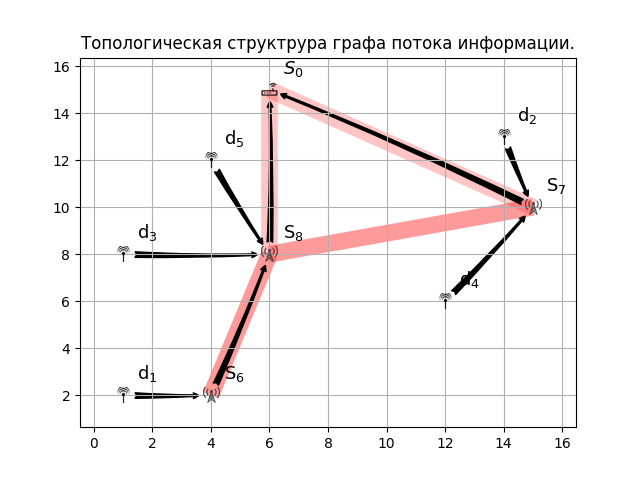
\includegraphics[width=.8\textwidth]{lp_solution.png}
    \caption{Допустимое решение.}
    \label{fig:part3_lp_solution}
\end{figure}

Теперь можно решить задачу ЛП \cref{eq:part2_1.1, eq:part2_1.2, eq:part2_1.3, eq:part2_1.4_1, eq:part2_1.4_2, eq:part2_1.5}. На рисунке \cref{fig:part3_lp_solution} представлен полученный граф допустимого решения. Жирными линиями представлена телекоммуникационная связь между объектами и БС. Стрелками указан полученный граф потока информации от объектов до шлюза. Математическая модель была подготовлена на языке Python, задачи ЛП была рассчитана с использованием библиотеки с открытым исходным кодом NetworkX \cite{networkx}. 

% \fixme{проверить текст}

% может быть применена стандартная процедура нахождения допустимого решения задачи линейного программирования с вводом искусственных переменных в уравнения \cref{eq:part2_1.1, eq:part2_1.2, eq:part2_1.3, eq:part2_1.4_1, eq:part2_1.4_2} и минимизации состоящей из этих переменных линейной формы. Если значение целевой функции в результате решения задачи окажется больше нуля, то допустимого решения для данного размещения станций не существует, в противном случае полученное решение дает допустимое распределение потоков по каналам связи.

% Далее мы рассмотрим понятие базисных структур в контексте BCMCFPR. В отличие от сетевого симплексного алгоритма для традиционной задачи потока с минимальными затратами (см. [2, стр. 405–407]), нам нужно отказаться от предположения, что подграф, индуцированный базовыми ребрами, не имеет циклов. Вместо этого в основе лежит цикл с ненулевой платой за использование, как это будет подробно показано ниже. 



% \fixme{================================================================}

% \fixme{После получения, матрицы смежности $H$ необходимо, убедиться, что данный граф является связным. Хотя может это и проверяем в ЛП. Пока так оставить}

% \fixme{ПРОВЕРИТЬ Задача о потоке минимальной стоимости}
% \fixme{Примем допущение, что интенсивность везде одинакова и равна $\lambda$ . Потом умножить на средий размер пакетов.}
% \fixme{Проверить идею кратчайшего остовного дерева. Проверить как считает стоимости}
% \fixme{================================================================}


\FloatBarrier
\section{Математическая модель оптимальной задачи выбора набора размещаемых БС и определения мест их размещения}

В параграфе будет представлена оптимизационная задача размещения типов БС БШС для обеспечения телекоммуникационного покрытия рассредоточенных объектов. Задача имеет ту же постановку как в модели ЛП, теперь  только множество вершин $A_2$ задаются свободными. Необходимо разместить БС из заданного множества типов БС для развертывания БШС на плоскости.

\subsection{Постановка задачи.}

Задано множество вершин $A = \{a_i\}$, $i=\overline{0,n}$ на некоторой территории. Каждая вершина $a_i$ имеет координаты $\left\{ x_i, y_i \right\}$.
Множество $A$ состоит из двух подмножеств: $A_1 = \left\{a_i \right\}, i= \overline{1,n_1}$ множество вершин, с которых необходимо собирать информацию; $A_2 = \left\{ a_i  \right\}, i= \overline{n_1+1,n}$ множество возможных мест размещения БС. 

% \begin{itemize}
%     \item $A_1$ -- множество вершин, с которых необходимо собирать информацию;
%     \item $A_2$ -- множество возможных мест размещения БС. 
% \end{itemize}

% Каждой вершине $a_i$ приписана   величина $v_i$ -- максимальный объем информации, снимаемой с объекта, расположенного на этой вершине.

% По определению

% $$
% A_1 \cup A_2 = A;
% $$

% $$
% A_1 \cap A_2 = \varnothing.
% $$

% Все вершины пронумерованы так, что:

% $$
% A_1 = \left\{a_i \right\}, i= \overline{1,n_1};
% $$

% $$
% A_2 = \left\{ a_i  \right\}, i= \overline{n_1+1,n}.
% $$


Задано множество типов БС $S = \{s_j$\}, $j=\overline{1,m}$ для размещения на множестве точек $A_2$. Каждому типу БС приписаны четыре параметра $s_j = \left\{\{r_{ji}\}, \{R_{ji}\}, \vartheta_j, c_j \right\}$, где: 
\begin{itemize}
    \item $\{r_{ji}\}$ множество радиусов покрытия. Параметр $r_{ji}$ характеризует телекоммуникационную связь для обеспечения соединения между $j$-ой станцией и объектом, размещенный в координате $a_i$, $j= \overline{n_1+1,n}$, $i= \overline{1,n_1}$;
    \item $\{R_{ji}\}$ радиус связи между $j$-ой и $i$-ой станциями. Параметр характеризует максимальную дальность связи $j$-ой станции, обеспечивающее заданное качество соединения с $i$-ой станцией, $j= \overline{n_1+1,n}$, $i= \overline{n_1+1,n}$, $j \neq i$;
    \item $\vartheta_j$ пропускная способность;
    \item $c_j$ стоимость.
\end{itemize}

% максимальный объем информации в единицу времени, который может быть получен от объектов, обслуживаемых данной станцией

Задана БС специального вида (шлюз) $s_0 = \left\{ \{R_{0j}\}, \vartheta_0 \right\}$ с координатами $\left\{x_0, y_0 \right\}$. Шлюз уже имеет свое расположение, стоимость размещения $c_0 = 0$. Параметр шлюза $\{R_{0j}\}, j = \overline{n_1+1,n}$ радиус связи необходим для соединения с размещаемыми БС. Полагается, что шлюз не имеет соединения напрямую с объектами. По шлюз $s_0$ позволяет собрать данные со всех объектов, размещенных в точках $a_i$, $i= \overline{1,n_1}$, в данной постановке задачи пропускная способность шлюза равна $\vartheta_0 = \infty$.


Множества вершин $A_1$ будем идентифицировать как размещенные на них объекты. Множества вершин $A_2$, на которых будут размещены БС, будем рассматривать, непосредственно, как сами БС. 

Требуется разместить БС таким образом, чтобы вся информация с объектов на вершинах множества $A_1$ могла быть собрана и передана системой БС, размещенных на выбранных в результате решения задачи в вершинах множества  $A_2$, до шлюза $s_0$ и итоговая стоимость размещения была бы минимальной.

% \fixme{Вершин и станции будем, соответственно, идентифицировать как объекты или станции на них размещенные.}

Рассматривается MESH сеть. Задано условие, что информация с вершин множества $A_1$ может передаваться непосредственно только на вершины множества $A_2$, а со шлюзом и между собой могут быть связаны только вершины множества $A_2$.

\subsection{Модель частично целочисленного линейного программирования}

На этапе обследования местности проектировании БШС были отобраны точки, куда возможно расставить БС. Необходимо отметить, что при такой постановке на этапе синтеза топологии, рассматривается более общий случай, когда размещаются не множества имеющихся БС, а выбираются их типы. Так результатом данного этапа будут набор типов БС и их места размещения.

\subsubsection{Построение матрицы смежности}

На каждой вершине $a_i$, $i= \overline{n_1+1,n}$ может разместиться одна из $m$-типов БС. Вместо каждой такой вершины $a_i$ введем $m$ вершин с координатами вершины $\{x_i, y_i \}$, и различными параметрами, соответствующими различным типам БС. Обозначим такую группу вершин, записанных с одинаковыми координатами вместо вершины $a_i$, как $D_i$. Каждой вершине из $D_i$ поставим в соответствие набор параметров только одного типа БС из $S$, т.е. на вершине может стоять либо станция приписанного типа либо никакая. Обозначим расширенное множество вершин $A_2$ через $A_2D = \{a_i\}, i = \overline{n_1 + 1,\ n \cdot m}$.



Составим граф $H=\left\{AD,E\right\}$, описывающий сеть для передачи потока информации между вершинами расширенного множества $AD=A_1 \cup A_2D$ и шлюзом $s_0$ в вершине $a_0$.
Матрица смежности $E = \{e_{ij} \}$ графа $H$, где каждое ребро $e_{ij}$ определяет возможность передачи информации между вершинами, строится по следующим правилам. 

\begin{itemize}
    \item $e_{ij} = 1$, если расстояние между $i$-ой вершиной ($a_i \in A_1$) и $j$-ой вершиной ($a_j \in A_2D$) не более радиуса покрытия $r_{ji}$, приписанного этой вершине станции;
    \item $e_{ij} = 1$, если вершины $a_i$ и $a_j$ принадлежат разным множествам $D_i$ и $D_j$ и расстояние между ними не больше минимального из радиусов связи $\min\{R_{ij}, R_{ji}\}$, приписанных данным вершинам станциям;
    \item $e_{i0} = 1$ ($a_i \in A_2D$), если расстояние от вершины до шлюза не больше минимального радиуса связей $\min\{R_{i0}, R_{0i}\}$;
    \item $e_{ij} = 0$, во всех остальных случаях.
\end{itemize}

\subsubsection{Формулировка в виде ЧЦЛП}

С помощью полученного графа потока опишем ограничения для задачи частично целочисленного линейного программирования (ЧЦЛП).

Введем булевы переменные $z_{ij} = \{0, 1\}$, $, i = \overline{1,n_1}, j = \overline{n_1+1, \ n \cdot m}$, определяющее наличие соединения между объектом в точке $a_i, a_i \in A_1$  и БС, размещенной в точке $a_j, a_j \in A_2D$.


Все объекты, размещенные на вершинах $A_1$, оснащены антеннами для передачи сигнала в беспроводной среде. Каждая объект одновременно может поддерживать соединение только с одной БС. Данной условие можно записать в виде ограничения равенства \cref{eq:part3_only_1_link_from_device}

% Распишем условия для нашей задачи.
% Величина суммарного потока, который выходит с вершины $a_i$ равен весу $\vartheta_i$ \cref{eq:part2_1.5}

\begin{equation}\label{eq:part3_only_1_link_from_device}
    \sum_{a_j \in \Gamma_2^+(a_i)} z_{ij} = 1, \forall a_i, i =\overline{1, n_1},
\end{equation} 
где $\Gamma^+(a_i)$ -- множество вершин на графе $H$, в которые входят дуги, исходящие из вершины $a_i$.

Введем потоковые переменные $x_{ij} \in \mathbb{R}^+$, определяющее количество информации, передаваемой в единицу времени по дуге $e_{ij}$ графа $H$.

Потоки информации объектов с вершин $A_1$ должны поступать на станции. Также на станции может поступать потоки с других БС. Необходимо, чтобы сумма входящих и выходящих потоков для любой $j$-ой вершины множества $A_2D$ был равен нулю \cref{eq:part3_sta_io_flows} 
% \fixme{проверить индексы}
\begin{equation}\label{eq:part3_sta_io_flows} 
    \sum_{a_i \in \Gamma_1^-(a_j)} z_{ij} \cdot \vartheta_i + \sum_{a_i \in \Gamma_2^-(a_j)} x_{ij} -  \sum_{a_i \in \Gamma_2^+(a_j)} x_{ji} =0 ,\forall a_j \in A_2. 
\end{equation} 

% todo: delete this comment
% \begin{equation}\label{eq:part3_sta_io_flows} 
%     \sum_{a_j \in \Gamma_1^-(a_i)} z_{ij} \cdot \vartheta_i + \sum_{a_j \in \Gamma_2^-(a_i)} x_{ji} -  \sum_{a_j \in \Gamma_2^+(a_i)} x_{ij} =0 ,\forall a_i \in A_2. 
% \end{equation} 

Здесь множество $\Gamma_1^-(a_i)$ -- вершины множества $A_1$, из которых выходят дуги, входящие в вершину $a_i$; $\Gamma_2^-(a_i)$ -- вершины множества $A_2D$, из которых выходят дуги, входящие в  вершину $a_i$; $\Gamma_2^+(a_i)$ -- вершины множества $A_2D$, в которые входят дуги, исходящие из вершины  $a_i$.

Через систему БС вся информация от объектов  должна поступить на шлюз $s_0$ \cref{eq:part3_device2gateway_flow} 
\begin{equation}\label{eq:part3_device2gateway_flow}
    \sum_{a_j \in \Gamma_2^-(a_0)} x_{j0} = \sum_{a_i \in A_1} \vartheta_i,
\end{equation}
здесь $\Gamma_2^-(a_0)$ –- подмножество вершин множества $A_2D$, дуги которых входят в шлюз $a_0$.

Введем булевы переменные $y_{ij} = \{0,1\}$ для потока $x_{ij}$, исходящего из вершины $a_i$, $a_i \in A_2D$ в вершину $a_j$, $a_j \in A_2D$. Данная переменная характеризует наличие соединения между вершинами.
% \begin{itemize}
%     \item $y_i = 1$, если станция стоит на месте $a_i$;
%     \item $y_i = 0$, в противном случае.
% \end{itemize}

% Объем информации, поступающей от вершин множества $A_1$ на вершину $a_i \in A_2D$, ограничен мощностью станции $\vartheta_i$ \cref{eq:part2_1.8}
Поток информации $w_{ij}$ между вершинами множества $A_2D$ может передаваться только при наличии соединения $y_{ij}$. Также данный поток ограничен пропускной способностью $\vartheta_i$ БС  \cref{eq:part3_flow_link_sta}
\begin{equation}\label{eq:part3_flow_link_sta}
    \sum_{a_j \in \Gamma_2^-(a_i)} x_{ij} \leqslant y_{ij} \cdot \vartheta_i, \forall a_i \in A_2D.
\end{equation}

Каждая БС может иметь только одно соединение для передачи потока информации в единицу времени. Необходимо обеспечить условие, что в каждом множестве $D_i$ может быть размещено не более одной станции. Оба этих требования можно записать в виде ограничения неравенства \cref{eq:part3_only_1_link_yij}

\begin{equation}\label{eq:part3_only_1_link_yij}
    \sum_{a_j \in \Gamma_2^-(a_i)} y_{ij} \leqslant 1, \forall D_i.
\end{equation}

Целевая функция задачи минимизации стоимости размещения \cref{eq:part3_of_min}

\begin{equation}\label{eq:part3_of_min}
    \sum_{a_i \in A_2D} \sum_{a_j \in \Gamma_2^-(a_i)}c_i \cdot y_{ij} \to min.
\end{equation}

Задача \cref{eq:part3_only_1_link_from_device, eq:part3_sta_io_flows, eq:part3_device2gateway_flow, eq:part3_flow_link_sta, eq:part3_only_1_link_yij, eq:part3_of_min} представляет собой частично целочисленную задачу линейного программирования с $m \cdot |A_2|$ булевыми переменными. 

\subsubsection{Пример решения задачи ЧЦЛП}

Рассмотрим пример для оптимизационной задачи выбора набора размещаемых БС и определения мест их размещения.
Задано множество рассредоточенных объектов $A_1$, $|A_1| = 8$, параметры которых представлены в таблице \cref{tab:part3_mip_devices}, и множество точек возможного размещения БС \cref{tab:part3_mip_station_coordinates} Рисунок \cref{fig:part3_mip_input_data}). 
Задано множество типов БС $S, |S| = 2$ (таблица \cref{tab:part3_mip_station_types}). 
Задана станция специального вида -- шлюз с параметрами, представленными в таблице  \cref{tab:part3_mip_gateway}. Необходимо разместить БС таким образом, чтобы вся информация с объектов могла быть собрана и  передана на шлюз и с учетом бюджетного ограничения. 

\begin{figure}[h!]
    \centering
     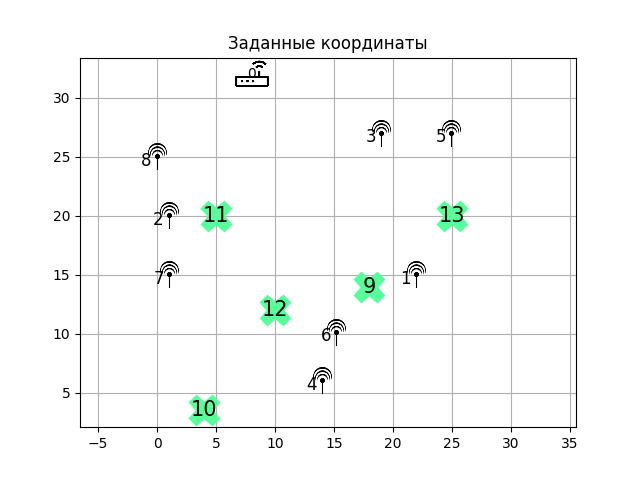
\includegraphics[width=.8\textwidth]{mip_input_data.png}
  \caption{Множество $A$.}
  \label{fig:part3_mip_input_data}
\end{figure}



Вместо каждой такой вершины $a_i$ из множества возможных точек размещения БС $A_2$ необходимо ввести $|S| =2 $ вершин с координатами точки $a_i$ и различными параметрами, соответствующими различным типам БС. Полученное расширенное множество $A_2D$ представлено в таблице \cref{tab:part3_mip_station_point}.


\begin{table}[h!]\centering
    \begin{tabular}{|c||c|c|c|c|c|}\hline
        
        Точки размещения & \multirow{2}{*}{Координаты} & \multirow{2}{*}{$\vartheta$}	&\multirow{2}{*}{$P_{tr}$}&	\multirow{2}{*}{$G_{tr}$}& \multirow{2}{*}{$L$}\\

        станций, $A_2$& & & & & \\
        \hline
        \textnumero & м & 1/с & дБм& дБ& дБ\\
        \hline
        $a_1$& (22, 15)& 11 & 10&	1&	0 \\
        $a_2$& (1, 20)& 11 & 10&	1&	0 \\
        $a_3$& (19, 27)& 11 & 10&	1&	0 \\
        $a_4$& (14, 6)& 12 & 10&	1&	0 \\
        $a_5$& (25, 27)& 13 & 10&	1&	0 \\
        $a_6$& (15.2, 10.1)& 15 & 10&	1&	0 \\
        $a_7$& (1, 15)& 17 & 10&	1&	0 \\
        $a_8$& (0, 25)& 19 & 10&	1&	0 \\
    
        \hline
  
  \end{tabular}\caption{Рассредоточенные объекты}\label{tab:part3_mip_devices}
\end{table}


\begin{table}[h!]\centering
    \begin{tabular}{|c||c|}\hline
        
        $A_2$& Координаты\\
        \hline
        $a_9$& (18, 14) \\
        $a_{10}$& (4, 3.5) \\
        $a_{11}$& (5, 20) \\
        $a_{12}$& (10, 14) \\
        $a_{13}$& (25, 20) \\
       
        \hline
  
  \end{tabular}\caption{Точки размещения станций}\label{tab:part3_mip_station_coordinates}
\end{table}



\begin{table}[h!]\centering
    \begin{tabular}{|c||c|c|c|c|c|c|}\hline
        
        S& $\vartheta$	&$P_{tr}$&	$G_{tr}$&	$P_{recv}$ &$L$ & $c$\\
        \hline
        \textnumero & 1/c & дБм&	дБ&	дБм&	дБ & у.е.\\
        \hline
        $s_1$& 1300 & 20&	4&	-79& 1& 70\\
        $s_2$& 1400& 18&	3&	-81& 1 & 80\\

        \hline
  
  \end{tabular}\caption{Типы станций}\label{tab:part3_mip_station_types}
\end{table}

\begin{table}[h]\centering
    \begin{tabular}{|c||c|c|c|c|c|c|}\hline
        
        Шлюз& Координаты & $\vartheta$	&$P_{tr}$&	$G_{tr}$&	$P_{recv}$ &$L$\\
        \hline
        \textnumero & м & 1/c & дБм&	дБ&	дБм& дБ\\
        \hline
        $s_0$&  (8, 32)& $\infty$ & 20&	4&	-79& 1\\
        \hline
  
  \end{tabular}\caption{Параметры шлюза}\label{tab:part3_mip_gateway}
\end{table}


% \fontsize{10pt}{10pt}\selectfont
\begin{table}[h]
    \begin{tabular}{|  c||  c|  c|  c|  c|  c|  c|  c|  c|  c|  c|}
    

    \hline
    \tiny
    Множество $A_2$&\multicolumn{2}{c|}{$a_9$}&\multicolumn{2}{c|}{$a_{10}$}&\multicolumn{2}{c|}{$a_{11}$}& \multicolumn{2}{c|}{$a_{12}$}&\multicolumn{2}{c|}{$a_{13}$} \\
    \hline
    Множество типов станций $S$&$s_1$& $s_2$&$s_1$& $s_2$& $s_1$& $s_2$& $s_1$& $s_2$& $s_1$& $s_2$  \\
    \hline
    Расширенное множество $A_2D$&$a_9$& $a_{10}$&$a_{11}$&$a_{12}$& $a_{13}$& $a_{14}$& $a_{15}$& $a_{16}$& $a_{17}$& $a_{18}$  \\
  
    \hline
    \end{tabular}
    \caption{Расширенное множество $A_2D$}\label{tab:part3_mip_station_point}
\end{table}
\normalsize

Используя уравнения потерь в свободном пространстве и уравнение энергетического баланса необходимо рассчитать радиус телекоммуникационного покрытия и радиус связи станций, чтобы получить граф потока $H$. Запас на замирание сигнала $SOM = 30$ и несущая частота $f=5537$. В таблице \cref{tab:part3_mip_adj_mat} представлена матрица смежности $E$ полученного графа $H$.


\begin{table}[hbt!]
    \tiny
    \begin{tabular}{| c|| c| c c c c c c c c| c c c c c c c c c c|}

    \hline

    &$a_0$ &$a_1$ &$a_2$ &$a_3$ &$a_4$ &$a_5$ &$a_6$ &$a_7$ &$a_8$ &$a_9$& $a_{10}$&$a_{11}$&$a_{12}$& $a_{13}$& $a_{14}$& $a_{15}$& $a_{16}$& $a_{17}$& $a_{18}$  \\
    \hline \hline
    $a_0$ & 0 &0 &0 &0 &0 &0 &0 &0 &0 &0 &0 &0 &0 &0 &0 &0 &0 &0 &0  \\
    \hline
    $a_1$ & 0 &0 &0 &0 &0 &0 &0 &0 &0 &1 &1 &0 &0 &0 &0 &0 &0 &1 &1  \\
    $a_2$ & 0 &0 &0 &0 &0 &0 &0 &0 &0 &0 &0 &0 &0 &1 &1 &0 &0 &0 &0  \\
    $a_3$ & 0 &0 &0 &0 &0 &0 &0 &0 &0 &0 &0 &0 &0 &0 &0 &0 &0 &1 &1  \\
    $a_4$ & 0 &0 &0 &0 &0 &0 &0 &0 &0 &1 &1 &1 &1 &0 &0 &1 &1 &0 &0  \\
    $a_5$ & 0 &0 &0 &0 &0 &0 &0 &0 &0 &0 &0 &0 &0 &0 &0 &0 &0 &1 &1  \\
    $a_6$ & 0 &0 &0 &0 &0 &0 &0 &0 &0 &1 &1 &0 &0 &0 &0 &1 &1 &0 &0  \\
    $a_7$ & 0 &0 &0 &0 &0 &0 &0 &0 &0 &0 &0 &1 &1 &1 &1 &1 &1 &0 &0  \\
    $a_8$ & 0 &0 &0 &0 &0 &0 &0 &0 &0 &0 &0 &0 &0 &1 &1 &0 &0 &0 &0  \\
    \hline
    $a_9$ & 1 &0 &0 &0 &0 &0 &0 &0 &0 &0 &1 &1 &1 &1 &1 &1 &1 &1 &1  \\
    $a_{10}$ & 1 &0 &0 &0 &0 &0 &0 &0 &0 &1 &0 &1 &1 &1 &1 &1 &1 &1 &1  \\
    $a_{11}$ & 1 &0 &0 &0 &0 &0 &0 &0 &0 &1 &1 &0 &1 &1 &1 &1 &1 &1 &1  \\
    $a_{12}$ & 1 &0 &0 &0 &0 &0 &0 &0 &0 &1 &1 &1 &0 &1 &1 &1 &1 &1 &1  \\
    $a_{13}$ & 1 &0 &0 &0 &0 &0 &0 &0 &0 &1 &1 &1 &1 &0 &1 &1 &1 &1 &1  \\
    $a_{14}$ & 1 &0 &0 &0 &0 &0 &0 &0 &0 &1 &1 &1 &1 &1 &0 &1 &1 &1 &1  \\
    $a_{15}$ & 1 &0 &0 &0 &0 &0 &0 &0 &0 &1 &1 &1 &1 &1 &1 &0 &1 &1 &1  \\
    $a_{16}$ & 1 &0 &0 &0 &0 &0 &0 &0 &0 &1 &1 &1 &1 &1 &1 &1 &0 &1 &1  \\
    $a_{17}$ & 1 &0 &0 &0 &0 &0 &0 &0 &0 &1 &1 &1 &1 &1 &1 &1 &1 &0 &1  \\
    $a_{18}$ & 1 &0 &0 &0 &0 &0 &0 &0 &0 &1 &1 &1 &1 &1 &1 &1 &1 &1 &0  \\
    \hline
    \end{tabular}\caption{Матрица смежности}\label{tab:part3_mip_adj_mat}
\end{table}

Решением задачи ЧЦЛП \cref{eq:part3_only_1_link_from_device, eq:part3_sta_io_flows, eq:part3_device2gateway_flow, eq:part3_flow_link_sta, eq:part3_only_1_link_yij, eq:part3_of_min} является размещение, представленное на рисунке \cref{fig:part3_mip_solution}. Были размещены базовые станции типы $s_3$ в точках $a_11$, $a_12$ и $a_13$. Жирным цветом представлены возможные соединения базовых станций, стрелками граф потока информации от объектов до шлюза. Математическая модель была подготовлена на языке Python, задача ЧЦЛП решалась в коммерческом продукте Gurobi Optimization.  Код программы представлен в \url{https://github.com/m0000Amir/BSP-on-plane}.

\begin{figure}[hbt!]
    \centering
     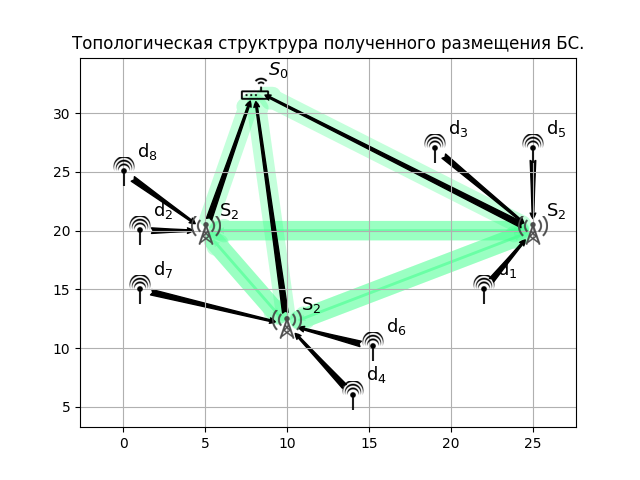
\includegraphics[width=.8\textwidth]{mip_solution.png}
  \caption{Решение задачи ЧЦЛП.}
  \label{fig:part3_mip_solution}
\end{figure}

\FloatBarrier
\section{Выводы по главе 3}

В работе рассмотрены задачи размещения базовых станций при проектировании беспроводных широкополосных сетей связи для покрытия множества рассредоточенных объектов. 
\begin{itemize}
    \item Предложена формулировка задачи в виде математической модели линейного программирования при заданных мест размещения станция для проверки условия допустимой передачи потока от множества объектов до точки корневого узла сети;
    \item Предложена математическая модель экстремальной задачи в виде частично целочисленного линейного программирования оптимального размещения станций из имеющегося набора типов станций на избыточном множестве возможных мест размещения;
    \item Предложены алгоритмы построения графа информационных потоков, позволяющие формализовать задачи в виде соответствующих моделей математического программирования. 
\end{itemize}

Результаты исследования по главе 3 были опубликованы в работах \cite{MukhtarovPershinGUBKIN2018_RSCI, 
MukhtarovPershinGUBKIN2019_RSCI,MukhtarovPershinVSPU2019_RSCI, MukhtarovPershinMLSD2019works_RSCI, MukhtarovPershinMLSD2019materials_RSCI,}. 




% В Приложении \cref{app:milp_place_solution} приведены результаты вычислительного эксперимента. 



\FloatBarrier

\chapter{Оценка характеристик производительности сети с помощью имитационного моделирования}\label{prediction_model}

Проектирования БШД в связи с высокой сложностью и вычислительными трудностями требует поэтапного подхода учета всего комплекса критериев качества и ограничений для проектируемой беспроводной сети.

После решения задачи синтеза топологии, для полученного размещения решаются задачи оцненки качества. Такими задачами являются расчет надежности всех элементов сети, оценка характеристик качества канала, вероятности потери пакетов, пропускной способности, времени доставки сообщений в сети. Данный комплексный подход позволяет дать  
Одной из важных задач на стадии проектировании является оценка производительности широкополонсой беспроводной сети. 

======

\cite{Tcharo2018} 

Здесь будет имитационная модель сети массового обслуживания и методы машинного обучения.


В работе \cite{Eremenko2013} рассматривают стохастическую модель марковской цепи для оценки качества предоставления информационных услуг передачи данных АСУ ТП в условиях помех и прерываний.

\section{Аппроксимация функций распределений случайных величин}
\section{Имитационная модель с зависимым обслуживанием}
\begin{figure}[h!]
  \centering
   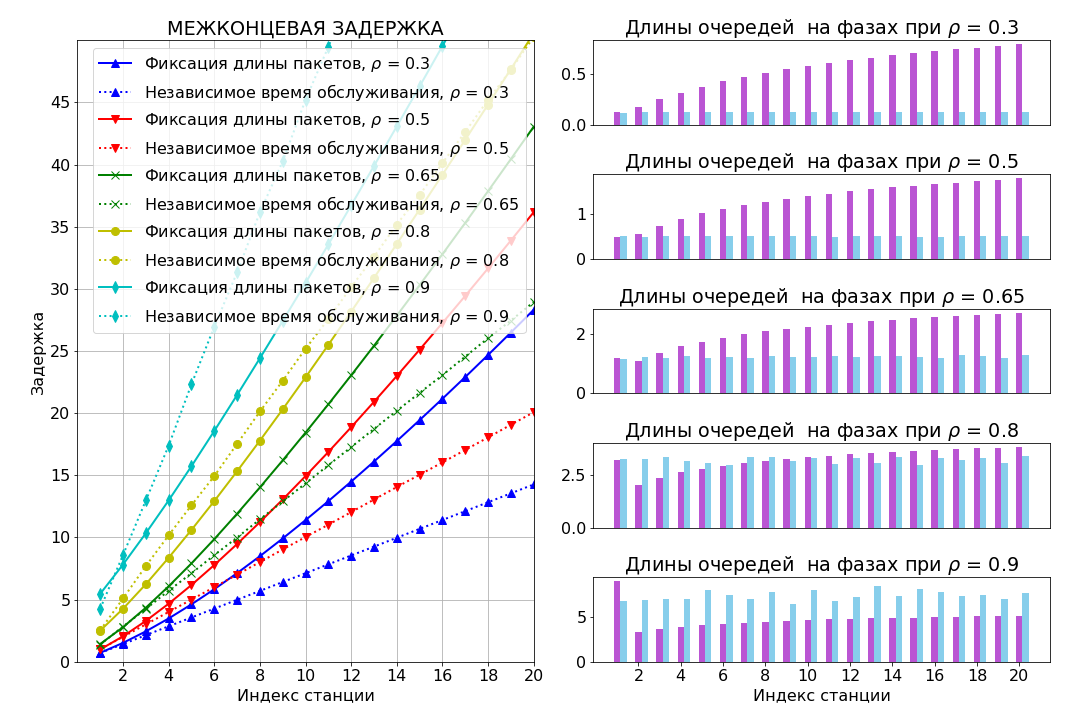
\includegraphics[width=0.8\textwidth]{sim20_model.png}
\caption{Задержки для случаев с независимой и зависимой функции распределения времени обслуживания}
\label{fig:sim20_model}
\end{figure}

\section{Модели прогноза времени межконцевой задеркжи с помощью методов машинного обучения}
\begin{figure}[h!]
    \centering
     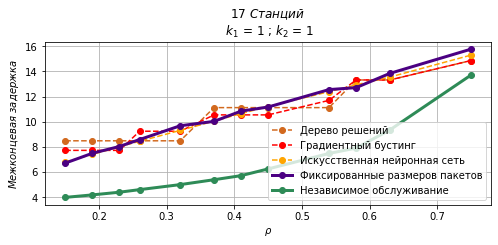
\includegraphics[width=0.8\textwidth]{17predict_model.png}
  \caption{Оценки времени межконцевых задержек для тандема размером 17}
  \label{fig:17predict_model}
\end{figure}

\section{Выводы по главе \cref{prediction_model}}


% \chapter{Математические модели синтеза топологии сети для охвата линейного участка в виде экстремальной задачи в комбинаторной форме}\label{chapter_combinatorial_model}

% Эффективным способом повышения технико-экономических показателей при проектировании \fixme{БШС} является оптимизация топологии сети, а именно решение задачи выбора оптимального набора станций из заданного избыточного множества и определение мест их размещения вдоль линейной контролируемой территории.
% Основным результатом работы, представленной в этой главе, является разработка итерационного метода выбора оптимальной топологии сети в процессе комплексного проектирования БШС. 
% Принципиальной особенностью предлагаемого метода, повышающей его эффективность, является то, что для рассмотрения на этапе моделирования предлагается не одно решения, а последовательности лучших решений задачи оптимизации топологии сети. Это позволяет с помощью разработанной итерационной процедуры выбирать на этапе моделирования лучшее решение среди тех решений по топологии, которые удовлетворяют требуемым характеристикам проектируемой БШС. 

% \section{Постановка задачи и ее формулировка в экстремальной комбинаторной форме}

% Пусть задано множество станций $S=\{s_j\}$ с параметрами $s_j=\{r_j,\{R_{jq} \},\mu_j, c_j \},j=1,...,m;q=1,...,m;j \neq q $. Здесь $r_j$ -- максимальный радиус покрытия станции, $\{R_{jq} \}$ -- множество максимальных радиусов связи между $j$-ой и $q$-ой базовой станции, $\mu_j$ - интенсивность времени обслуживания и $c_j$ -- стоимость станции.

% Задана максимальная допустимая стоимость размещенных станций $C$. 


% Задан отрезок $\alpha$ длиной $L$ с концами в точках $a_0$ и $a_{n+1}$. Внутри отрезка $\alpha = [a_0, a_{n+1}]$ задано множество возможных точек размещения станций множества $A=\{a_i \},i=1,...,n$ c координатами $l_i$.Точка $a_0$ имеет координату $l_0=0$, точка $a_{n+1}$ имеет координату $l_{n+1}=L$. На концах отрезка, в вершинах $a_0$ и $a_{n+1}$, стоят станции специального вида $s_0$ и $s_{m+1}$, соответственно, для которых радиусы покрытия, пропускные способности и стоимости не задаются. Радиусы связи задаются как $R_{0j}$ и $R_{(m+1)j}$, соответственно.
% Требуется разместить станции таким образом, чтобы максимизировать размер контролируемой ими территории (покрытие) отрезка $L$ при выполнении требования наличия связи каждой станции со станциями на концах отрезка (шлюзами) через систему размещенных станций при выполнении ограничений на время межконцевой задержки $T$ и суммарную стоимость размещенных станций $C$.
% Сформулируем задачу в виде экстремальной задачи на конечном множестве.

% \textit{Допустимой расстановкой станций} назовем такой возрастающий по величине координат $l_i$  набор пар $P = \{a_i, s_j\},a_i \in A,i \neq 0,i \neq n+1;s_j \in S$, для которого выполняются требования:

% % \begin{enumerate}
% % 	\item left connectivity: $\forall\;(a_i, s_j),\,1 \leq i \leq n,$ either $\exists (a_k, s_q):\:l_k < l_i $ 
% % 	and $l_i - l_k \leq \min \{R_j, R_q \},$ or $l_i - l_0 \leq R_j$;
% % 	\item right connectivity: $\forall\;(a_i, s_j),\,1 \leq i \leq n,$ either $\exists (a_t, s_g):\:l_t > l_i $ 
% % 	and $ l_t - l_i \leq \min \{R_j, R_g \}, $ or $ l_{n+1} - l_i \leq R_j$;	
% % 	\item $|P| = m$.
% % \end{enumerate}
% \begin{enumerate}
%     \item  для каждой пары $(a_i,s_j)$:
%         \begin{enumerate}
%             \item слева: либо найдется такая пара $(a_k,s_q)$, что, $l_i - l_k \leqslant R_{jq}$  и $l_i - l_k  \leqslant R_{qj}$, либо $l_i-l_0 \leqslant R_{j0}$ и $l_i - l_0 \leqslant R_{0j}$;
%             \item справа: либо найдется такая пара $(a_t,s_g)$, что, $l_t-l_i \leqslant R_{jq}$ и $l_t - l_i \leqslant R_{qj}$, либо $l_{n+1}-l_i \leqslant R_{j(m+1)}$ и $l_{n+1}-l_i \leqslant R_{(m+1)j}$. 
%         \end{enumerate}
% % - слева: либо найдется такая пара (a_k,s_q), что, l_i-l_k≤R_jq  и l_i-l_k  ≤R_qj, либо l_i-l_0≤R_j0 и l_i-l_0≤R_0j;
% % - справа: либо найдется такая пара (a_t,s_g), что, l_t-l_i≤R_jq и l_t-l_i  ≤R_qj, либо l_(n+1)-l_i≤R_(j(m+1)) и l_(n+1)-l_i≤R_((m+1)j). 
% Данное требование гарантирует, что любая станция может быть связана со станциями на концах отрезка либо через промежуточные станции, либо непосредственно;
%     \item в одной точке стоит не более одной станции;
%     \item сумма задержек по всем размещенным станциям меньше заданной величины $T$ – средней межконцевой задержки по времени по всей системе станций:
%     \begin{displaymath}
%         \label{eq:part3_e2e_delay}
%         \sum\limits_{j \in S_\sigma} \overline{T_j} \leqslant T,
%     \end{displaymath}
% где $S_\sigma$ – множество размещенных станций, $\overline{T_j}$ -- среднее время задержки на станции. Расчет задержек описан в параграфе \cref{part4_e2e_delay_section}
%     \item суммарная стоимость размещенных станций меньше заданного бюджетного ограничения  $C$.
% \end{enumerate}

% Каждой допустимой расстановке станций $P$ соответствует величина покрытия $z(P)$, определяемая как суммарная длина всех таких участков $\tau,\tau \subset \alpha$, что каждая точка этих 
% участков попадает в зону покрытия, по крайней мере, одной станции, входящей в набор пар $P$.

% Для удобства описании в дальнейшем алгоритмов введем понятие «недопокрытия» отрезка $\alpha$:

% \begin{displaymath}
%     f(P) = L - z(P)
% \end{displaymath} 

% Пусть $G$ -- множество всех допустимых расстановок $P$.
% Тогда мы можем сформулировать нашу задачу в следующей комбинаторной форме экстремальной задачи на конечном множестве. 

% \textbf{Задача 1.}

% Требуется найти такую допустимую расстановку  $P^*$, что
% \begin{equation}
%     \label{eq:part3_P}
%     P^* = \argmin \limits_{P \in G} f(P)
% \end{equation}

% Обозначим через $\Gamma$ все множество вариантов размещения станций (не обязательно допустимых) из множества $S$ на заданном множестве возможных мест их размещения.

% \section{Дерево ветвлений для перебора элементов в множестве \texorpdfstring{$\Gamma$}{Lg}}

% Опишем процедуру построения бинарного дерева поиска (дерева ветвлений) для полного перебора без повторений всех элементов множества $\Gamma$. Данная процедура будет использована в дальнейшем при построении дерева поиска в алгоритме МВиГ решения \textbf{задачи 1}.

% В дальнейшем будем предполагать, что в множестве $S$ станции упорядочены по не убыванию радиусов покрытия. 
% Описываемая процедура использует известный прием разбиения множества $G$ на подмножества с использованием некоторого параметра. Процесс формирования и последовательность исследования подмножеств обычно представляется с помощью дерева поиска, представляющего собой ориентированное от корня «дерева ветвлений», где каждому подмножеству соответствует вершина на дереве. Множеству $\Gamma$ соответствует корневая вершина. 

% \subsection{Параметр для разбиения множеств на подмножества}
% \textit{\textbf{Процедура 1.}}

% Пусть $G_0$, где нижний индекс – номер итерации, исходное множество $\Gamma$. На каждой итерации, начиная с итерации $\nu=0$, разбиваем текущее подмножество $G_\nu$ на два подмножества $G^1_\nu$ и $G^2_\nu$. При этом множество $G_\nu$ обычно называется «материнским», а множества $G^1_\nu$  и $G^2_\nu$  - «потомками» множества $G_\nu$ или дочерними узлами.

% В качестве параметра разбиения воспользуемся переменной $\pi_{ij}$, принимающей два значения 0 и 1:

% \begin{itemize}
%     \item $\pi_{ij}=1$, если наложено условие, что на месте $a_i$ расположена станция $s_j$;
%     \item $\pi_{ij} = 0$, если наложено условие, что на месте $a_i$ станция $s_j$  располагаться не будет.
% \end{itemize}

% В дальнейшем будем считать, что для множества $G^1_\nu$ задано условие $\pi_{ij}=1$, а для множества $G^2_\nu$  задано условие $\pi_{ij} = 0$.

% Очевидно, что

% \begin{equation}
%     \label{eq:part4_G_cup}
%     G^1_\nu \cup G^2_\nu = G_\nu;
% \end{equation}


% \begin{equation}
%     \label{eq:part4_G_cap}
%     G^1_\nu \cap G^2_\nu = \varnothing.
% \end{equation}

% Выбор переменной для разбиения на $\nu$-ой итерации

% На этапе разбиения любого множества $G_\nu$ все множество переменных $\Pi = \{\pi_{ij}\}$ можно разделить на три подмножества: множество $\Pi^+$ -- «фиксированные» переменные, для которых $\pi_{ij}=1$, множество $\Pi^-$ -- «запрещенные» переменные, для которых $\pi_{ij}=0$, и множество $\Pi^f$ -- «свободные» переменные, для которых значения на данной итерации еще не заданы.

% Правило выбора переменной для разбиения множества $G_\nu$. Для разбиения множества $G_\nu$ на данной итерации выбирается из множества $\Pi^f$ переменная c наименьшим индексом $j$ среди всех переменных с наименьшим индексом $i$. Таким образом сначала определяется незанятое место размещения $a_i$ с наименьшим номером (индексом $i$) и на нем размещается еще не размещенная станция $s_j$ с наименьшим номером (индексом $j$).

% \subsection{Движение по дереву ветвлений}

% После разбиения очередного подмножества $G_\nu$ два подмножества $G^1_\nu$  и $G^2_\nu$, последним на дереве ветвлений присваиваются порядковые индексы $G_{\nu+1}$ и $G_{\nu+2}$, соответственно.
% При формировании дерева ветвлений различаются два типа шагов: «прямой» шаг и «обратный» шаг. Прямой шаг -- это движение «в глубину» по той же ветви дерева, реализующее очередное разбиение множества $G_\nu$ на два потомка, и обратный шаг, реализующий переход от множества $G_\nu$  к одному из ранее сформированных подмножеств. Обратный шаг делается в том случае, когда либо получено множество $G_\nu$, состоящее из единственного элемента, либо множество $G_\nu$  при данном наборе значений переменных $\pi_{ij}$, выделяющих данное подмножество $G_\nu$ из множества $G_0$, пусто. В этих случаях соответствующая вершина дерева называется «закрытой».

% Для движения по дереву будем использовать правило \fixme{LIFO}. На основании этого правила прямые шаги будут выполняться до тех пор, пока не будет получена закрытая вершина. На дереве ветвлений это соответствует продолжению движения по той же ветви дерева. При этом из двух множеств $G^1_\nu$  и $G^2_\nu$ первым будет исследоваться на возможность закрытия соответствующей вершины множество $G^1_\nu$. Если вершина в результате проведенного исследования не будет закрыта, то из неё будет продолжено дальнейшее движение по той же ветви (выполнение прямого шага). Если вершина будет закрыта, то будет выполнен обратный шаг: для дальнейшего рассмотрения и продолжения движения будет выбрана незакрытая вершина с наибольшим порядковым номером $\nu$ среди всех висячих вершин дерева (последняя сформированная вершина из нерассмотренных). Процедура будет завершена, когда все вершины дерева будут закрыты.

% Заметим, что выполнение условий \cref{eq:part4_G_cup, eq:part4_G_cap} гарантирует, что в результате завершения работы \textit{\textbf{процедуры 1}} будут просмотрены все элементы множества $\Gamma$ без повторений. Эти же условия определяют фундаментальное свойство дерева ветвлений: на каждой итерации объединение множеств $G_\nu$ всех висячих вершин дерева дает исходное множество $G_0$ корневой вершины.


% \subsection{Алгоритм метода ветвей и границ} \label{BnB}
% Для построения алгоритма \fixme{МВиГ} для решения \textbf{задачи 1} с использованием \textit{\textbf{процедуры 1}} для построения дерева ветвлений нам достаточно разработать методы исследования вершин дерева на возможность их закрытия.
% В соответствии с техникой \fixme{МВиГ} закрытие вершины в результате исследования, соответствующего ей множества $G_\nu$ возможно в трех случаях.

% \underline{\textit{\textbf{Случай 1.}}} Множество $G_\nu$ -- пусто, т.е. доказано, что в множестве $G_\nu$ при данном наборе фиксированных и запрещенных переменных $\pi_{ij}$ нет ни одной допустимой расстановки $P$.

% \underline{\textit{\textbf{Случай 2.}}} Доказано, что в множестве $G_\nu$ не может быть допустимой расстановки P с меньшим значением целевой функции (1), чем у лучшей расстановки $\widehat{P}$ из уже найденных. Значение функции $f(\widehat{P})$ называется «рекордом», а расстановка $\widehat{P}$ -- «рекордным решением». В качестве начального рекорда принимается число заведомо большое искомого оптимального решения, например, $L$ – длина всего отрезка.

% \underline{\textit{\textbf{Случай 3.}}} Найдено оптимальное решение \textbf{задачи 1} на множестве $G_\nu$.
% Прежде чем рассмотреть эти три случая, запишем важное свойство любого множеств $G_\nu$, являющееся следствием принятого правила выбора свободной переменной для разбиения очередного множества $G_\nu$ при прямом шаге. 

% \textit{\textbf{Свойство 1.}} Пусть для исследуемого множества $G_\nu, \nu > 0$, точка $a_k$ -- это одно любое из мест, на которых уже размещены станция из множества $S$ в соответствии с набором фиксированных и запрещенных переменных $\pi_{ij}$, выделяющим данное множество из множества $G_0$. Тогда для всех мест «слева» от $a_k$, т.е. точек $a_i$, $i<k$, размещение станций уже определенно (при этом некоторые места могут быть пустыми).
% Перейдем непосредственно к исследованию \underline{\textit{\textbf{случаев 1 – 3}}}.

% \underline{\textit{\textbf{Случай 1.}}}

% Проверка текущего множества $G_\nu$ на пустоту состоит в установлении факта невозможности выполнения требований 1) – 4) введенных ранее при определении допустимой расстановки.

% Рассмотрим проверку условия выполнения требования 1) для множества $G_\nu, \nu > 0$. 

% Пусть множество $G_\nu$  образовано разбиением материнского множества при помощи переменной $\pi_{kt}=1$. Проверяем, что каждый из радиусов $R_{th}$ и $R_{ht}$, где $h$ – индекс станции, размещенной на ближайшей слева к точке $a_k$ точке $a_d$ больше расстояния $l_k-l_d$. Если ближайшая слева точка – это точка $a_0$ (левый конец отрезка $\alpha$), то делается проверка, для радиуса $R_{t0}$ и $R_{0t}$. 

% Если данное условие не выполняется, то множество $G_\nu$ недопустимо, соответствующая вершина закрывается и делается шаг обратного хода в соответствии с \textit{\textbf{процедурой 1}}. 

% Если множество $G_\nu$ образовано разбиением материнского множества при помощи переменной $\pi_{kt}=0$ и $a_d$ -- точка с наибольшим индексом, среди точек, на которых уже размещены станции (точки $a_0$, если размещенных станций нет), то надо проверить, что среди нераспределенных станций, без учета станции $s_t$, есть такая станция $s_q$ что расстояние между точками $a_k$ и $a_d$ не больше, чем $R_{qh}$ и $R_{hq}$. Если проверка отрицательна, то множество $G_\nu$ -- пусто, соответствующая этому множеству на дереве поиска вершина должна быть закрыта и выполняется шаг обратного хода в соответствии с  \textit{\textbf{процедурой 1}}.

% Требование 2) выполняется соответствующим выбором очередной станции для размещения, требования 3) и 4) выполняются непосредственным суммированием соответствующих параметров у размещенных станций.

% \underline{\textit{\textbf{Случай 2.}}}
% Построим оценку величины «недопокрытия» для множества $G_\nu$, полученного из материнского множества добавлением условия $\pi_{kt}=1$. Частичным «недопокрытием» назовем величину $\Delta(k,d,p,t)$, которая вычисляется по формуле:

% \begin{equation}\label{eq:part4_delta}
% \Delta(k,d,p,t) = max\{\left(a_{k} - a_{d} \right) - \left(r_{p} + r_{t} \right), 0\}.
% \end{equation}

% Частичное «недопокрытие» \cref{eq:part4_delta} определяется для любых двух точек $a_d$ и $a_k$,$k>d$, на которых расположены станции $s_p$ и $s_t$ при условии, что между этими точками нет других станций. Очевидно, что для любой расстановки $P$ «недопокрытие» $f(P)$ вычисляется как сумма всех «недопокрытий» $\Delta(k,d,p,t)$ между местами размещения станций, включая концы отрезка $\alpha$, на которых стоят станции особого типа $s_0$ и $s_{m+1}$.

% \begin{displaymath}
% W(G_\nu) \leq f(P), P \in G_\nu. 
% \end{displaymath}

% Если $W(G_\nu) \geq f(\widehat{P})$, то множество $G_\nu$ не может содержать расстановки лучше уже найденной расстановки $\widehat{P}$ соответствующая множеству $G_\nu$  вершина на дереве поиска должна быть закрыта и далее выполняется шаг обратного хода в соответствии с  \textit{\textbf{процедурой 1}}. 

% Построим оценку «недопокрытия» для множества $G_\nu$, полученного из материнского множества добавлением условия $\pi_{kt}=1$. Оценку будем искать в в
% иде суммы

% \begin{displaymath}
%     W\left(G_\nu\right) = w_1 + w_2. 
% \end{displaymath}

% Величина $w_1 \left(G_\nu \right)$ вычисляется как сумма все частичных «недопокрытий» слева от вершины $a_k$ и величины радиуса покрытия, размещаемой станций $r_t$. Оценку $w_2 \left(G_\nu \right)$ вычислим «для недопокрытия» справа на части $\beta$ до конца отрезка $\alpha$ (точки $a_{n+1}$). Данную оценку получим релаксацией условий, определяющих допустимую расстановку станций на участке $\beta$. Найдем такое подмножество $S_\beta$ множества станций $S$, состоящее из еще не размещенных станций и дающее минимальное «недопокрытие» на участке $\beta$ при выполнении только условий 2) – 4). Для этого сформулируем следующую задачу булевого программирования.

% \underline{\textit{\textbf{Задача 2.}}}
% \begin{displaymath}
%     z = |\beta| - \sum\limits_{x_j \in S_\beta} r_j x_j \rightarrow min.
% \end{displaymath}
% при условии:

% \begin{equation}\label{eq:part4_task2_cost}
%     \sum\limits_{x_j \in S_\beta} c_j x_j \leqslant C,
% \end{equation}

% \begin{equation}\label{eq:part4_task2_m}
%     \sum\limits_{x_j \in S_\beta} x_j \leqslant m,
% \end{equation}

% \begin{displaymath}
%     x_j \in \{0, 1\},
% \end{displaymath}
% где $|\beta|$ -- длина отрезка отрезка  $\beta$, $m$ -- число свободных мест для размещения станций на отрезке $\beta$.

% Очевидно, что эффективность использования оценки в методе ветвей и границ определяется точностью оценки и временем ее вычисления. \underline{\textit{\textbf{Задача 2}}} -- это задача ЦЛП, являющаяся труднорешаемой \cite{Gari}. На основании \underline{\textit{\textbf{задачи 2}}} можно получить две оценки менее точные, но имеющие более эффективные методы решения. Заметим, что при снятии ограничения \cref{eq:part4_task2_cost} или \cref{eq:part4_task2_m} \underline{\textit{\textbf{задача 2}}} представляет собой целочисленную задачу о ранце c эффективным псевдополиномиальным алгоритмом решения \cite{Gari}. При этом с точки зрения точности оценки, более перспективным представляется снятие ограничения \cref{eq:part4_task2_m}, так как на практике, обычно, число возможных мест размещения станций существенно меньше числа размещенных станций, полученного в результате решения задачи. Назовем задачу, полученную снятием ограничения \cref{eq:part4_task2_m}, \underline{\textit{\textbf{задачей 3}}}.

% \underline{\textit{\textbf{Задачу 2}}} при снятии условия целочисленности на переменные назовем \underline{\textit{\textbf{задачей 4}}}. \underline{\textit{\textbf{Задача 4}}} есть задача линейного программирования. Очевидно, что \underline{\textit{\textbf{задачи 3}}} и \underline{\textit{\textbf{задачи 4}}}, являясь оценками целевой функции решения \underline{\textit{\textbf{задачи 2}}}, могут служить оценками $w_2 (G_\nu)$. Результаты численного эксперимента с различными оценками вынесены в \fixme{приложение 2}.

% Если множество $G_\nu$ получено из материнского добавлением условия $\pi_{kt}=0$, то оценка $W(G_\nu)$ равна оценке материнского множества.

% \fixme{В приложении 1} приведены результаты вычислительного эксперимента, показывающего время решения \underline{\textit{\textbf{задач 2, 3, 4}}} и относительную точность \underline{\textit{\textbf{задачи 3 и 4}}} по отношению к \underline{\textit{\textbf{задаче 2}}}.

% Перейдем к рассмотрению \underline{\textit{\textbf{случая 3}}}. Рассматривается только для множеств $G_\nu$, состоящих из единственной расстановки $P$, для которой «недопокрытие» $f(P)$ вычисляется как сумма всех недопокрытий $\Delta(k,d,p,t)$ между местами, где размещены станций, включая концы отрезка $\alpha$, на которых стоят станции $s_0$ и $s_{m+1}$. 

% Если для найденной расстановки $P$ выполняются условия 1) – 4), которые для единственной расстановки легко проверяются, и

% \begin{equation}
%     \label{eq:part4_is_less_than_record}
%     f(P) < f(\widehat{P}),
% \end{equation}
% то $f(P)$ принимается за новый рекорд $f(\widehat{P})$, расстановка $P$ становиться новым рекордным решением $\widehat{P}$ и выполняется шаг обратного хода в соответствии с \textit{\textbf{Процедурой 1}}, если неравенство \cref{eq:part4_is_less_than_record} не выполняется, то рекорд остается прежним и выполняется шаг обратного хода.

% Работа алгоритма МВиГ заканчивается, когда все вершины дерева поиска закрыты, при этом решение задачи: 

% \begin{displaymath}
%     P^{*} = \widehat{P},  f(P^*) = f(\widehat{P}).
% \end{displaymath}

% \subsection{Построения последовательности топологий для итерационной процедуры моделирования \fixme{БШС}}

% В результате проектирования \fixme{БШС} надо найти ее оптимальную топологию среди всех топологий, для которых будут выполняться все требования к показателям, исследуемым и рассчитываемым на этапе моделировании сети. Для решения этой задачи воспользуемся идеей метода построения последовательности планов \cite{Emelichev}.

% Рассмотрим \textbf{задачу 1.}

% Требуется найти такую допустимую расстановку $P^*$, что

% \begin{displaymath}
%     f(P^*) = min \{f(P), P \in G \}.
% \end{displaymath}

% Построим для этой задачи последовательность $\Gamma = P^1, P^2, ... ,P^k$ допустимых расстановок (решений) множества $G$ для заданного $k$, где 
% \begin{align}
%     f(P^1) &= f(P^*), \nonumber  \\
%     f(P^2) &= extr\{ f(P), P \in G \ P^1 \}, \nonumber \\
%     ... \nonumber \\
%     f(P^k) &= extr\{ f(P), P \in G \ P^1 \cup P^2 \cup ... P^k \}, \nonumber 
% \end{align}

% В последовательности $\Gamma$ каждое решение не лучше предыдущего и не хуже последующего.

% Теперь воспользуемся следующей процедурой. Будем последовательно, начиная с первой расстановки, выполнять этап моделирования \fixme{БШС}. Очевидно, что как только мы получим расстановку, удовлетворяющую всем требованиям этапа моделирования, мы решим задачу нахождения оптимальной топологии среди всех топологий, для которых выполняются все требования к показателям, исследуемым и рассчитываемым на этапе моделировании сети. Действительно, для всех предыдущих расстановок эти условия не выполняются, а все последующие расстановки в последовательности $\Gamma$ не могут быть лучше по критерию $f(P)$.

% Обсудим вопрос как строить подобную последовательность на основании алгоритма \fixme{МВиГ}, описанного в параграфе \cref{BnB}. Заменив неравенство \cref{eq:part4_is_less_than_record} на нестрогое и записывая все рекорды, полученные в процессе работы алгоритма, мы, очевидно, получим последовательность расстановок, где каждая расстановка не хуже предыдущей и не лучше последующей. Для получения последовательности $\Gamma$ достаточно «перевернуть» полученную последовательность, где первый элемент станет последним.

% Недостатком такой процедуры является то, что для исследования на этапе моделирования будут отобраны только расстановки не хуже первого рекорда и среди них может не оказаться расстановки, удовлетворяющей критериям моделирования.
% Для расширения множества $\Gamma$ можно сделать следующее. Зададим условие. что в результате решения \textbf{задачи 1} мы хотим получить не только оптимальное решение, но и все решения не хуже оптимального на величину $d$. Для решения такого варианта задачи достаточно неравенство \cref{eq:part4_is_less_than_record} в алгоритме \fixme{МВиГ} заменить следующим неравенством 

% \begin{equation}
%     \label{eq:part4_is_less_than_record_d}
%     f(P) \leqslant f(\widehat{P}) + d,
% \end{equation}
% где $d = \varepsilon \cdot L > 0, \varepsilon$ -- заданное отклонение в процентах, и запоминать все рекорды, полученные в процессе решения задачи.

% На основании неравенства \cref{eq:part4_is_less_than_record_d} можно построить итерационную процедуру, увеличивая величину $d$, если при данном ее значении допустимого решения на этапе моделирования не найдено.
% В \fixme{приложение 2} представлены результаты численного примера.

% \subsection{Расчет межконцевой задержки}\label{part4_e2e_delay_section}

% Одной из основных характеристик проектируемой сети является ее межконцевая задержка. Рассмотрим беспроводную сеть как сеть массового обслуживания (СеМО) с кросс-трафиком и с узлами $M/M/1$. По теореме Бурке \cite{Burke1956} на выходе узла $M/M/1$, а значит на входе каждой последующей фазы тоже пуассоновский поток. Интенсивность на выходе каждой фазы равна суммарной интенсивности всех входящих потоков с интенсивностями $\lambda$.

% По формуле Литтла \cite{Little1961} можно рассчитать время задержки на фазе. Интенсивность времени обслуживания рассчитывается по формуле: 

% \begin{displaymath}
%     \mu_j = p_j / w,
% \end{displaymath}
% где: $p_j$ - пропускная спобоность $j$-ой станции, Мбит/с; $w$ - средний размер пакета, Мбит.

% Для каждой станции коэффициент загрузки равен:


% \begin{displaymath}
% \rho_j= \frac{\sum{\lambda}}{\mu_j} = \frac{q \cdot \lambda}{\mu_j} <1,
% \end{displaymath}

% где $q$ -- число входящих потоков. Условие $\rho_j<1$ является необходимым и достаточным условием существования стационарного режима функционирования \fixme{СеМО}.

% Тогда среднее время задержки по времени на каждой станции:

% \begin{displaymath}
%     \overline{T_j} = \frac{\rho_j}{1 - \rho_j} \cdot \frac{1}{q \cdot \lambda}.
% \end{displaymath}

% Тогда межконцевая задержки в сети равна

% \begin{equation}
%     \label{eq:end_to_end_delay}
%     T^{e2e}= \sum{\overline{T_j}}.
% \end{equation}

% \subsection{Выводы по Главе \cref{chapter_combinatorial_model}}

% В работе предложена методика проектирования беспроводной широкополосной сети для контроля линейной трассы с использованием итерационной процедуры построения последовательности лучших решений задачи выбора и размещения базовых станций при выполнении технологических условий на проектирование сети и ограничения на стоимость размещаемых станций. 

% Предложенная методика позволяет на этапе моделирования выбирать лучшее решение среди тех решений по выбору и размещению станций, которые удовлетворяют требованиям, предъявляемым к проектируемой сети.

% Процедура нахождения последовательности лучших решений задачи выбора и размещения базовых станций основана на разработанном алгоритме \fixme{МВиГ}.


% % First we shall build $W(G_0)$.

% % Since all the stations must be placed, then the maximum coverage of $\alpha$ is obtained in situations when  it would be possible to place all the stations without intersections of their coverage radiuses . Each station $s_j$ covers the segment of length 2$r_j$, therefore, a total non - coverage cannot exceed the value.

% % \begin{displaymath}
% % W\left(G_0\right) = \max{\left\{L-\sum_{j=1}^{m}{2r_j,0}\right\}}.                                                                                  
% % \end{displaymath}

% % Now we will define $W(G_\nu)$, $\nu > 0$ as the sum of partial sums $w_1$ and $w_2$. 

% % \begin{displaymath}
% % W\left(G_\nu\right) = w_1 + w_2.                                                                                  
% % \end{displaymath}

% % Suppose $G_\nu$ is obtained by splitting a parent set by setting the variable $\pi_{kt}$ = 1. Then $w_1$ is "non-coverage" of the segment from $a_0$ to $a_k$ while $w_2$ is non-coverage of the segment from $a_k$ to $a_{n+1}$.

% % The sum $w_1$ is calculated by formula (\ref{eq1}) by summing non-coverages between the places where stations have been placed already. 

% % The sum $w_2$ is calculated as

% % \begin{equation}\label{eq2}
% % w_2 = max\left\{\left(l_{n+1}-l_k\right)-\left(r_t+\sum_{j\in S_v}{2r_j}\right),0\right\},
% % \end{equation}
% % where $S_\nu$ is the set of unplaced stations. 

% % The formula (\ref{eq2}) is analogous to the formula (\ref{eq1}) except the fact, that it is applicable to the part of segment $\alpha$ which is to the right from the last place where any station has been placed.

% % If $\pi_{kt}$ = 0 the estimation $W(G_{\nu})$ remains unchanged after splitting.

% % \subsection{Case 3.}
% % In this case we review only sets $G_\nu$, which consist of a single placement $P$, and $f(P)$ is obtained as the sum of non-coverages $\Delta(k,d,p,t)$ between known places where  stations are placed.

% %  If for the given placement the inequality $f(P) < f(\widehat{P})$ takes place, then the placement $P$ becomes a new current best value $\widehat{P}$ and backward step is applied.
 
% % The branch and bound algorithm will stop when all the vertexes of the searching tree will be closed.
 
% % The solution is
% % \begin{displaymath}
% % P^{*} = \widehat{P},  \widehat{f}(P^*) = f(\widehat{P}).
% % \end{displaymath}

% % \section{Example 1}

% % \textit{Input data.}

% % The segment $\alpha$  with $L$ = 50, end points $a_0$  and  $a_4$  with coordinates $l_0$ = 0 and $l_4$= 50 is given. There are internal  points $a_1$, $a_2$, $a_3$ with coordinates $l_1$ = 20, $l_2$= 30, $l_3$=40.

% % The set of stations $S=\left\{s_j\right\}, j=1,2$  is given, where station $s_j$ has parameters: $r_1$ = 20, $R_1$ = 40; $r_2$ = 5, $R_2$ = 20. There are special stations $s_0$ and $s_4$, on the end points with $r_0$=$R_0$= 
% % $r_4$=$R_4$=0.

% % We have to find a feasible placement $P^*$, such that

% % \begin{displaymath}
% % P^* = \min \limits_{P \in G} f(P)
% % \end{displaymath}

% % The process of solving the problem is presented in the form of a binary search tree (see Fig.~\ref{fig2}).
 
% % The initial value of $f(\widehat{P})=L=50$, $G_0=G$.

% % The vertices of the tree indicated by $\emptyset$  correspond to the sets $G_\nu$ for which there are no feasible placements.

% % Two placements $P_1$ and $P_2$ were obtained as the current best solutions  with $f(P_1)=15$ and $f(P_2)=5$.

% % The optimal solution is $P^\ast=P_2,\ \ f\left(P^\ast\right)=f\left(P_2\right)=5$.

% % \begin{figure}
% % 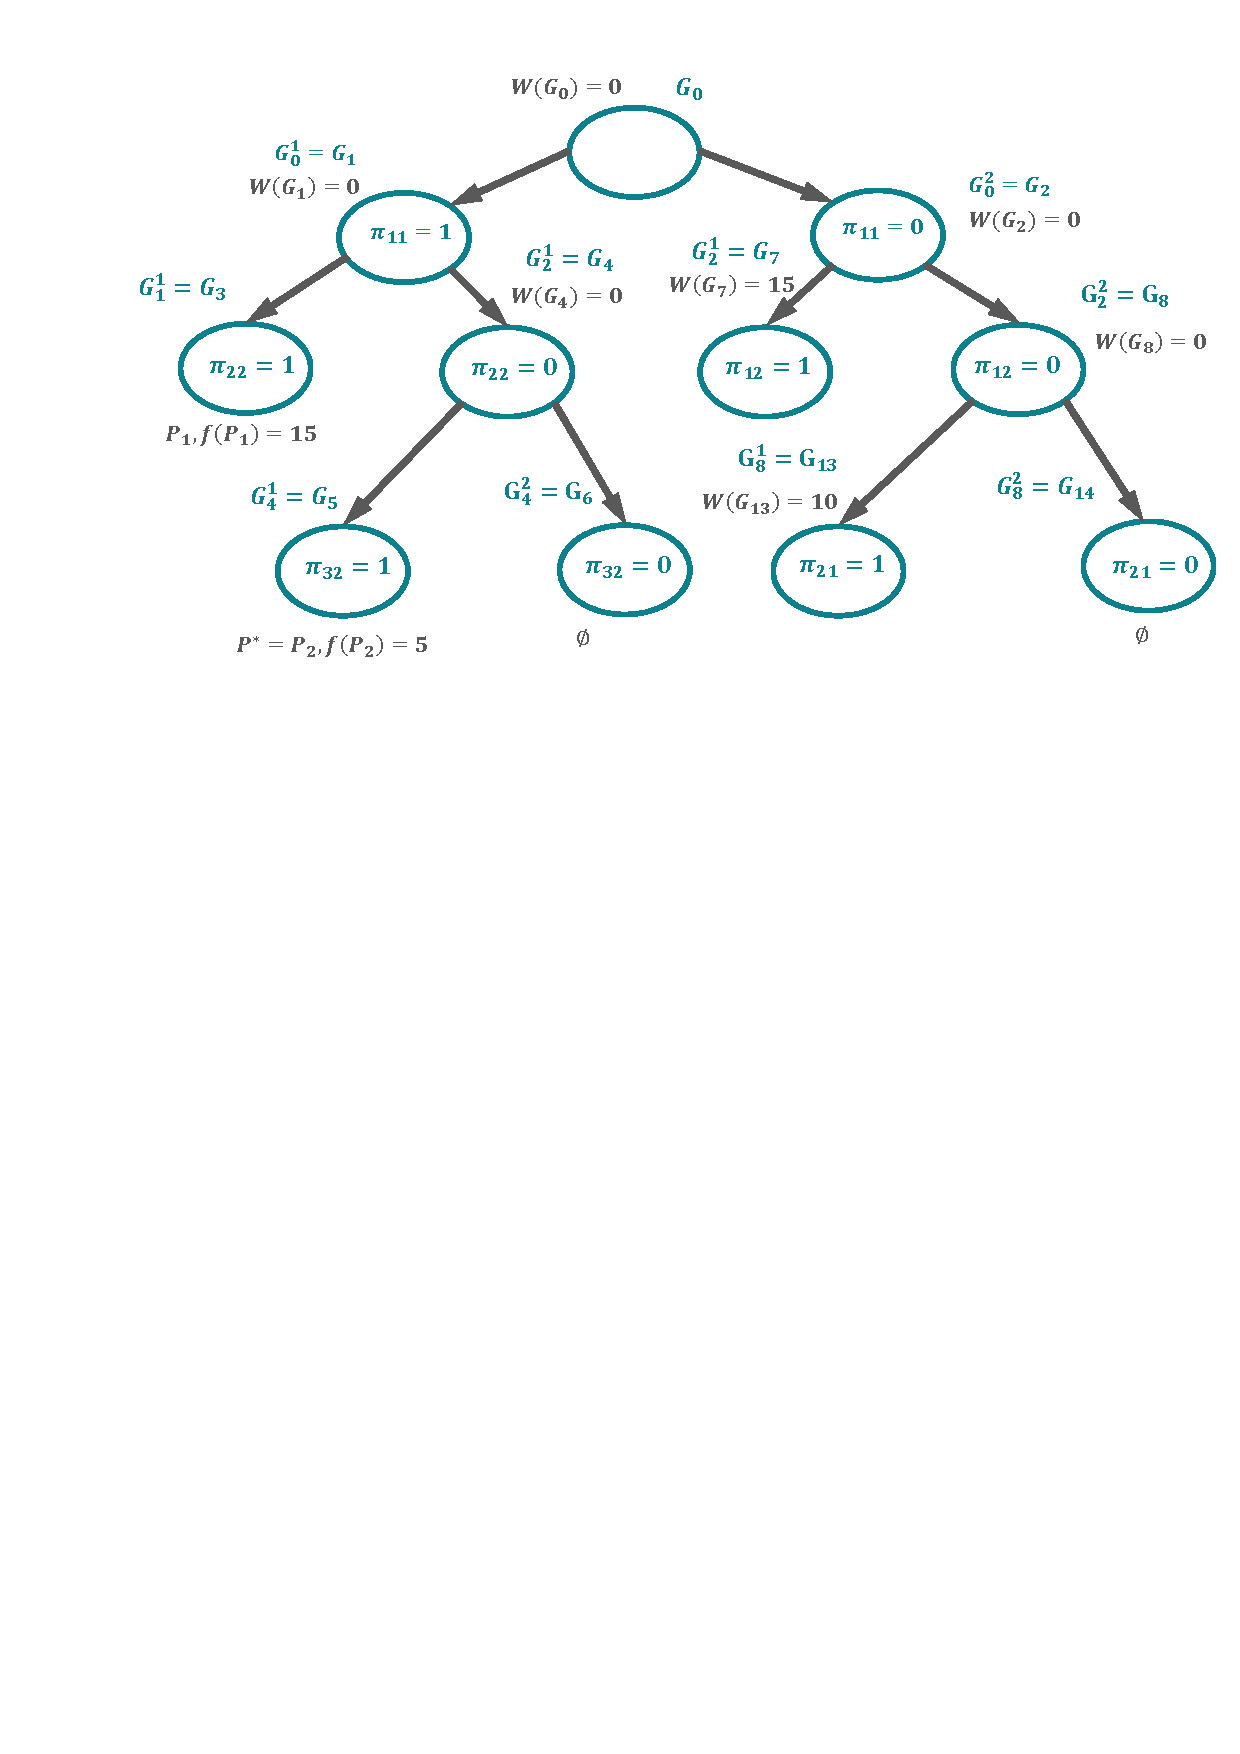
\includegraphics[width=\textwidth]{tree.pdf}
% % \caption{The search tree of branch and bound algorithm.} \label{fig2}
% % \end{figure}

% % \section{The statement of problem as a mixed – integer programming model}
% % Here we will formulate our placement problem in the form of a mixed – integer programming model. The description of problem is given in section 2.

% % Let us introduce binary variables $x_{ij}$ where $x_{ij}=1$ if a station $s_j$ is placed at point $a_i$ and $x_{ij}=0$ otherwise.

% % Let us introduce binary variables $e_i$ where $e_i$=1 if any station is placed at point $a_i$ and $e_i=0$ otherwise.

% % By definition

% % \begin{displaymath}
% % e_i=\sum_{j}^{m}{x_{ij}}, i=1,2,\ldots,n.
% % \end{displaymath}

% % We have $e_0$ = 1 and $e_{n+1}$ = 1 for the end points.

% % Let us formulate the following system of the problem constraints.

% % Each station must be placed in one and only one place

% % \begin{displaymath}
% % \sum_{i=1}^{n}{x_{ij}=1}, j=1,2,\ldots,m.
% % \end{displaymath}

% % At any point there can be no more than one station

% % \begin{displaymath}
% % \sum_{j=1}^{m}{x_{ij} \leq 1}, i=1,2,\ldots,m.
% % \end{displaymath}

% % We will introduce non-negative variables $y_i^+$  and  $y_i^-$ for points $a_i$, $i=0,1,2,..,n$, $n+1$.
% % Variables $y_i^+$ and  $y_i^-$  are the area sizes (right and left from point $a_i$) which are covered by station placed at point $a_i$.

% % Values of  variables $y_0^+$, $y_0^-$,$y_{n+1}^+$, $y_{n+1}^-$ equal 0.

% % The values of coverages are not greater than the coverage radius of the station located at $a_i$, and equal to 0 if is no station at $a_i$:

% % \begin{displaymath}
% % y_i^+\le\sum_{j=1}^{m}{x_{ij}r_j} ,i=1,2,\ldots,n,
% % \end{displaymath}

% % \begin{displaymath}
% % y_i^-\le\sum_{j=1}^{m}{x_{ij}r_j} ,i=1,2,\ldots,n.
% % \end{displaymath}

% % The total coverage area between any two points $a_i$ and $a_k$ on which the stations are located cannot exceed the distance between these points.

% % For  $i=1,\ldots,n$:

% % \begin{displaymath}
% % y_i^+ + y_k^- \le\frac{l_k - l_i}{2}\left(e_i + e_k\right)+\left(2 - e_i - e_k\right)L, k=i+1,\ldots,n+1,
% % \end{displaymath}

% % \begin{displaymath}
% % y_i^- + y_k^+  \le\frac{l_i - l_k}{2}\left(e_i + e_k\right)+\left(2 - e_i - e_k\right)L ,k=i-1,\ldots,0.
% % \end{displaymath}

% % 	This condition excludes the effect from intersections of station coverages when calculating the total coverage value for the entire segment $\alpha$.
	
% % 	According to the conditions of the problem, the station located at $a_i$ must be connected with at least one station on the left and one station on the right, including stations  at the end points $a_0$ and $a_{n+1}$.

% % 	We will introduce variables $z_{ijk}, i=1,2,\ldots,n$; $j=1,2,\ldots,m$; $k=1,2,\ldots,n$; $k\neq i$ to formulate this requirement where:

% % \begin{itemize}
% % 	\item $z_{ijk}=1$ if a station $s_j$ is located at point $a_i$ and connected with a station which is located at point  $a_k$;
% % 	\item $z_{ijk}=0$ otherwise.
% % \end{itemize}	
	
% % 	We will also introduce variables $z_{ij0}$ and $z_{ijn+1}$ where $z_{ij0}=1$ if a station $s_j$ is located at point $a_i$ and connected with a station $s_0$ which is located at point  $a_0$  and $z_{ij0} = 0$ otherwise; $z_{ijn+1}=1$ if a station $s_j$ is located at point $a_i$ and connected with a station $s_{n+1}$ which is located at point $a_{n+1}$  and $z_{ijn+1} = 0$ otherwise.

% % Stations must be at both points so that they can be connected: 

% % \begin{displaymath}
% % z_{ijk}\le e_i,  \forall i,j,k,
% % \end{displaymath}

% % \begin{displaymath}
% % z_{ijk}\le e_k, \forall i,j,k.
% % \end{displaymath}

% % The station $s_j$ which is located at $a_i$ must be connected with at least one station which is located right from $a_i$ and at least one station  which is located left from $a_i$

% % \begin{displaymath}
% % \sum_{k=i+1}^{n+1}{z_{ijk} \geq x_{ij}}, \forall i,j,
% % \end{displaymath}

% % \begin{displaymath}
% % \sum_{k=0}^{i-1}{z_{ijk} \geq x_{ij}}, \forall i,j.
% % \end{displaymath}

% % The communication radius $R_j$ of the station located at the point  $a_i$, must be no less than the distance to the point $a_k$, where there is a station with which it is connected:

% % \begin{displaymath}
% % z_{ijk\ }\left(R_j-\left(a_i-a_k\right)\right)\geq 0, k=i-1,\ldots,0, j=1,2,\ldots,m,  
% % \end{displaymath}

% % \begin{displaymath}
% % z_{ijk}\left(R_j-\left(a_k-a_i\right)\right)\geq 0, k=i+1,\ldots,n+1, j=1,2,\ldots,m. 
% % \end{displaymath}

% % Objective function

% % \begin{displaymath}
% % f=\sum_{i=1}^{n}{\left(y_i^++y_i^-\right)\rightarrow max} 
% % \end{displaymath}


% % \section{Numerical results}
% % The algorithms Branch and Bound (BnB) and brute-force algorithm (BF) were implemented using Python.
% % Table 1 shows the results of solving several problems for a different number of locations and a different number of stations using the B and B algorithm, the BF algorithm and the standard program for solving mixed – integer problem in the MATLAB package. We compare the number of vertices in the search trees so that the execution parameters of the algorithms do not depend on the speed of the machine and/or the quality the computer program. For each set of stations and set of placements   10 examples were computed with different numerical input data. For B and B and the MATLAB package the table shows the average execution parameters of the number of vertices in the search tree for each of the 10 examples.

% % \begin{table}
% % \caption{The results of solving problems.}\label{tab1}
% % \begin{tabular}{|l|l|l|l|l|}
% % \hline
% % {\bfseries Places} & {\bfseries Stations} &	{\bfseries BF}& {\bfseries BnB} & {\bfseries MILP} \\ 
% % \hline
% % 7 &		5 &	17550  &	933 &		753\\
% % 9 &		5 &	71090  &	6478 &		2669\\
% % 10 &	5 &	126180 &	1041 &		8551\\
% % 12 &	6 &	No &		8294 &		38569\\
% % 13 & 	6 &	No &		18485 &		30369\\
% % \hline
% % \end{tabular}
% % \end{table}

% % \textit {The numerical results. “No” means the problem was not solved after 3 hours}. 

% % \section{Conclusion}

% % In this  paper the problem of finding optimal location for the  given set of base stations in wireless network with linear topology was analyzed. The problem has been formulated as an  extremal combinatorial problem and also as mixed – integer linear programming model.  The branch and bound algorithm for solving the problem in combinatorial form was developed. The results of the computer experiment show that the branch and bound algorithm is more effective than the brute-force algorithm and using of the branch and bound algorithm also more effective than to solve the problem represented as a mixed–integer programming model.

% \include{Dissertation/part5}             % Глава 3
\chapter*{Заключение}                       % Заголовок
\addcontentsline{toc}{chapter}{Заключение} 
Создание и развитие современной структуры передачи данных являются неотъемлемой частью произвоздства. В рамках комплексного проектирования беспроводных средств связи в данной работе исследуются проблемы синтез топологии беспроводных сетей связи.

Основные результаты данного диссертационного исследования следующие:
\begin{enumerate}
    \item Проведен анализ методики проектирования современных БШС. В рамках такой методики были исследованы проблемы синтеза топологии БШС вдоль протяженных транспортных магистралей: автомобильные дороги, трубопроводные магистрали, лини метрополитена и т.д. 
    \item Предложена новая математическая модель в виде задачи ЦЛП оптимального размещения БС с линейной топологией.
    \item Представлена новая математическая модель задачи оптимального размещения БС в комбинаторной форме. 
    % Данная модель учитывает специфику задачи для нахождения оптимального решения.
    \item Для комбинаторной модели был разработан новый специальный алгоритм типа ветвей и границ. 
    
    % Представлены результаты сравнения поиска оптимального решения с помощью МВиГ с алгоритмами решения задачи в общем виде.
    \item В рамках комплексного проектирования БШС представлена новая итерационная процедура нахождения последовательности лучших решений задачи оптимального размещения БС для случая, когда найденное оптимальное решение построение топологии сети не удовлетворяет некоторым критериями функционирования БШС, проверяемых на следующих этапах проектирования.
    \item Предложена новая математическая модель виде задачи ЧЦЛП оптимального размещения БС для покрытия множества рассредоточенных объектов. 
    \item Разработан программный комплекс для расчета задачи оптимального размещения БС  с помощью предложенного алгоритма типа ветвей и границ.
    \item Представлены результаты численных экспериментов, доказывающие эффективность предложенных моделей и методов для решения задачи синтеза топологии при проектировании БШС.
\end{enumerate}


Поставленные в начале данной диссертационной работы цели были достигнуты, а соответствующие им задачи решены. В качестве перспектив дальнейшего исследования можно выделить следующие:
\begin{itemize}
    \item внедрение программных реализаций в состав итерационной процедуры комплексного проектирования беспроводных сетей связи;
    \item  применение предложенного МВиГ в решении более общих   задач оптимального размещения базовых станций, в которых кроме межконцевой задержки необходимо учитывать также  другие характеристики производительности БШС;
    \item исследование влияний реальной среды на физический уровень канала передачи данных для расчета оценок дальности телекоммуникационной связи.
    
\end{itemize}



% Добавляем его в оглавление

%% Согласно ГОСТ Р 7.0.11-2011:
%% 5.3.3 В заключении диссертации излагают итоги выполненного исследования, рекомендации, перспективы дальнейшей разработки темы.
%% 9.2.3 В заключении автореферата диссертации излагают итоги данного исследования, рекомендации и перспективы дальнейшей разработки темы.
%% Поэтому имеет смысл сделать эту часть общей и загрузить из одного файла в автореферат и в диссертацию:

% Основные результаты работы заключаются в следующем.
% %% Согласно ГОСТ Р 7.0.11-2011:
%% 5.3.3 В заключении диссертации излагают итоги выполненного исследования, рекомендации, перспективы дальнейшей разработки темы.
%% 9.2.3 В заключении автореферата диссертации излагают итоги данного исследования, рекомендации и перспективы дальнейшей разработки темы.

\begin{enumerate}
    \item Проведен анализ методики проектирования современных БШС. В рамках такой методики были исследованы проблемы синтеза топологии БШС вдоль протяженных транспортных магистралей: автомобильные дороги, трубопроводные магистрали, лини метрополитена и т.д. 
    \item Предложена новая математическая модель в виде задачи ЦЛП оптимального размещения БС с линейной топологией.
    \item Представлена новая математическая модель задачи оптимального размещения БС в комбинаторной форме. 
    % Данная модель учитывает специфику задачи для нахождения оптимального решения.
    \item Для комбинаторной модели был разработан новый специальный алгоритм типа ветвей и границ. 
    
    % Представлены результаты сравнения поиска оптимального решения с помощью МВиГ с алгоритмами решения задачи в общем виде.
    \item В рамках комплексного проектирования БШС представлена новая итерационная процедура нахождения последовательности лучших решений задачи оптимального размещения БС для случая, когда найденное оптимальное решение построение топологии сети не удовлетворяет некоторым критериями функционирования БШС, проверяемых на следующих этапах проектирования.
    \item Предложена новая математическая модель виде задачи ЧЦЛП оптимального размещения БС для покрытия множества рассредоточенных объектов. 
    \item Разработан программный комплекс для расчета задачи оптимального размещения БС  с помощью предложенного алгоритма типа ветвей и границ.
    \item Представлены результаты численных экспериментов, доказывающие эффективность предложенных моделей и методов для решения задачи синтеза топологии при проектировании БШС.
\end{enumerate}

% \begin{enumerate}
%     \item Был проведен анализ методики проектирования современных БШС. В рамках такой методики были исследованы проблемы синтеза топологии БШС вдоль протяженных участков: трубопроводные магистрали, протяженные автомобильные дороги. 
%     \item Была предложена математическая модель в виде задачи ЦЛП размещения БС с линейной топологией.
%     \item Была представлена математическая модель экстремальной задачи оптимального размещения БС в комбинаторной форме. 
%     % Данная модель учитывает специфику задачи для нахождения оптимального решения.
%     \item Для комбинаторной модели был разработан специальный алгоритм типа ветвей и границ. Представлены результаты сравнения поиска оптимального решения с помощью МВиГ с алгоритмами решения задачи в общем виде.
%     \item В рамках комплексного проектирования была представлена итерационная процедура нахождения последовательности лучших решений задачи оптимального размещения для случая, когда найденное оптимальное решение построение топологии сети не удовлетворяет некоторым критериями функционирования БШС, проверяемых на этапе моделирования процесса передачи данных.
%     \item Предложена математическая модель оптимального размещения БС для покрытия множества рассредоточенных объектов.
%     \item Разработан программный комплекс для расчета задачи оптимального размещения БС  с помощью предложенного алгоритма типа ветвей и границ.
% \end{enumerate}




% \begin{enumerate}
%   \item построены математические модели в виде экстремальной комбинаторной задачи и задачи ЦЛП для оптимального размещения базовых станций при проектировании БШС с линейной топологией;
%   \item представлен алгоритм метода ветвей и границ для задачи размещения базовых станций с линейной топологией; 
%   \item разработана итерационная процедура нахождения последовательности лучших решений для задачи размещения базовых станций в рамках комплексного проектирования БШС с линейной топологией;
%   \item разработаны математические модели для задач проектирования БШС для покрытия множества рассредоточенныз объектов;
%   \item разработаны модели прогнозирования оценок характеристик производительности сети с помощью методов машинного обучения.
% \end{enumerate}

% И какая-нибудь заключающая фраза.

% Последний параграф может включать благодарности.  В заключение автор
% выражает благодарность и большую признательность научному руководителю
% Иванову~И.\,И. за поддержку, помощь, обсуждение результатов и~научное
% руководство. Также автор благодарит Сидорова~А.\,А. и~Петрова~Б.\,Б.
% за помощь в~работе с~образцами, Рабиновича~В.\,В. за предоставленные
% образцы и~обсуждение результатов, Занудятину~Г.\,Г. и авторов шаблона
% *Russian-Phd-LaTeX-Dissertation-Template* за~помощь в оформлении
% диссертации. Автор также благодарит много разных людей
% и~всех, кто сделал настоящую работу автора возможной.
      % Заключение
\printnomenclature[3.5cm] % Значение ширины столбца с обозначениями стоит подбирать вручную
\nomenclature{БПЛА}{беспилотный летательный аппарат}
\nomenclature{БШС}{беспроводная широкополосная сеть}
\nomenclature{МВиГ}{метод ветвей и границ}
\nomenclature{МПП}{метод полного перебора}
\nomenclature{ЦЛП}{целочисленное линейное программирование}
\nomenclature{БС}{базовая станция}
% 5G сеть

\nomenclature{URLLC}{Ultra-Reliable and Low Latency Communications, cверхнадежная передача данных с малой задержкой}
\nomenclature{URLLC}{Ultra-Reliable and Low Latency Communications, cверхнадежная передача данных с малой задержкой}
\nomenclature{UL}{Up Link, восходящая линия связи}
\nomenclature{DL}{Down Link, нисходящая линия связи}

% TODO:  чекнуть все сокращения
\nomenclature{ТМО}{теория массового обслуживания}
\nomenclature{МО}{машинное обучение}
\nomenclature{EIRP}{Equivalent Isotropically Radiated Power, эффективная изотропно-излучаемая мощность передатчика}
\nomenclature{SOM}{System Operating Margin, запас на замирание сигнала}
\nomenclature{FSPL}{Free Space Path Loss, уравнение потерь в свободном пространстве}
\nomenclature{QoS}{Quality Of Service, качество обслуживания}

\nomenclature{СеМО}{сеть массового обслуживания}
\nomenclature{ИТС}{интеллектуальная транспортная система}
\nomenclature{VANET}{Vehicular Ad Hoc network, автомобильная самоорганизующаяся сеть}
\nomenclature{RSU}{Roadside Unit, придорожные стационарные объекты телекоммуникационной связи}

\nomenclature{V2V}{Vehicle-To-Vehicle, беспроводная связь для обмена данными между движущимися транспортными средствами}


\nomenclature{V2X}{Vehicle-To-Infrastructure, беспроводная связь для обмена данными между транспортным средством и инфраструктурой}

\nomenclature{LIFO}{Last Input, First Out, последним пришёл — первым ушёл}
\nomenclature{ЛП}{линейное программирование}
\nomenclature{ЧЦЛП}{частично целочисленное линейное программирование}        % Список сокращений и условных обозначений
\chapter*{Словарь терминов}             % Заголовок
\addcontentsline{toc}{chapter}{Словарь терминов}  % Добавляем его в оглавление

\textbf{TeX} : Cистема компьютерной вёрстки, разработанная американским профессором информатики Дональдом Кнутом

\textbf{панграмма} : Короткий текст, использующий все или почти все буквы алфавита
      % Словарь терминов
\clearpage                                  % В том числе гарантирует, что список литературы в оглавлении будет с правильным номером страницы
%\hypersetup{ urlcolor=black }               % Ссылки делаем чёрными
%\providecommand*{\BibDash}{}                % В стилях ugost2008 отключаем использование тире как разделителя
\urlstyle{rm}                               % ссылки URL обычным шрифтом
\ifdefmacro{\microtypesetup}{\microtypesetup{protrusion=false}}{} % не рекомендуется применять пакет микротипографики к автоматически генерируемому списку литературы
\insertbibliofull                           % Подключаем Bib-базы: все статьи единым списком
% Режим с подсписками
%\insertbiblioexternal                      % Подключаем Bib-базы: статьи, не являющиеся статьями автора по теме диссертации
% Для вывода выберите и расскомментируйте одно из двух
%\insertbiblioauthor                        % Подключаем Bib-базы: работы автора единым списком 
%\insertbiblioauthorgrouped                 % Подключаем Bib-базы: работы автора сгруппированные (ВАК, WoS, Scopus и т.д.)
\ifdefmacro{\microtypesetup}{\microtypesetup{protrusion=true}}{}
\urlstyle{tt}                               % возвращаем установки шрифта ссылок URL
%\hypersetup{ urlcolor={urlcolor} }          % Восстанавливаем цвет ссылок
      % Список литературы
\clearpage
\ifdefmacro{\microtypesetup}{\microtypesetup{protrusion=false}}{} % не рекомендуется применять пакет микротипографики к автоматически генерируемым спискам
\listoffigures  % Список изображений

%%% Список таблиц %%%
% (ГОСТ Р 7.0.11-2011, 5.3.10)
\clearpage
\listoftables   % Список таблиц
\ifdefmacro{\microtypesetup}{\microtypesetup{protrusion=true}}{}
\newpage           % Списки таблиц и изображений (иллюстративный материал)

\setcounter{totalchapter}{\value{chapter}} % Подсчёт количества глав

%%% Настройки для приложений
\appendix
% Оформление заголовков приложений ближе к ГОСТ:
\setlength{\midchapskip}{20pt}
\renewcommand*{\afterchapternum}{\par\nobreak\vskip \midchapskip}
\renewcommand\thechapter{\Asbuk{chapter}} % Чтобы приложения русскими буквами нумеровались

\chapter{Свидетельство о регистрации программы для ЭВМ}


\begin{figure}[ht]
    \centerfloat{
        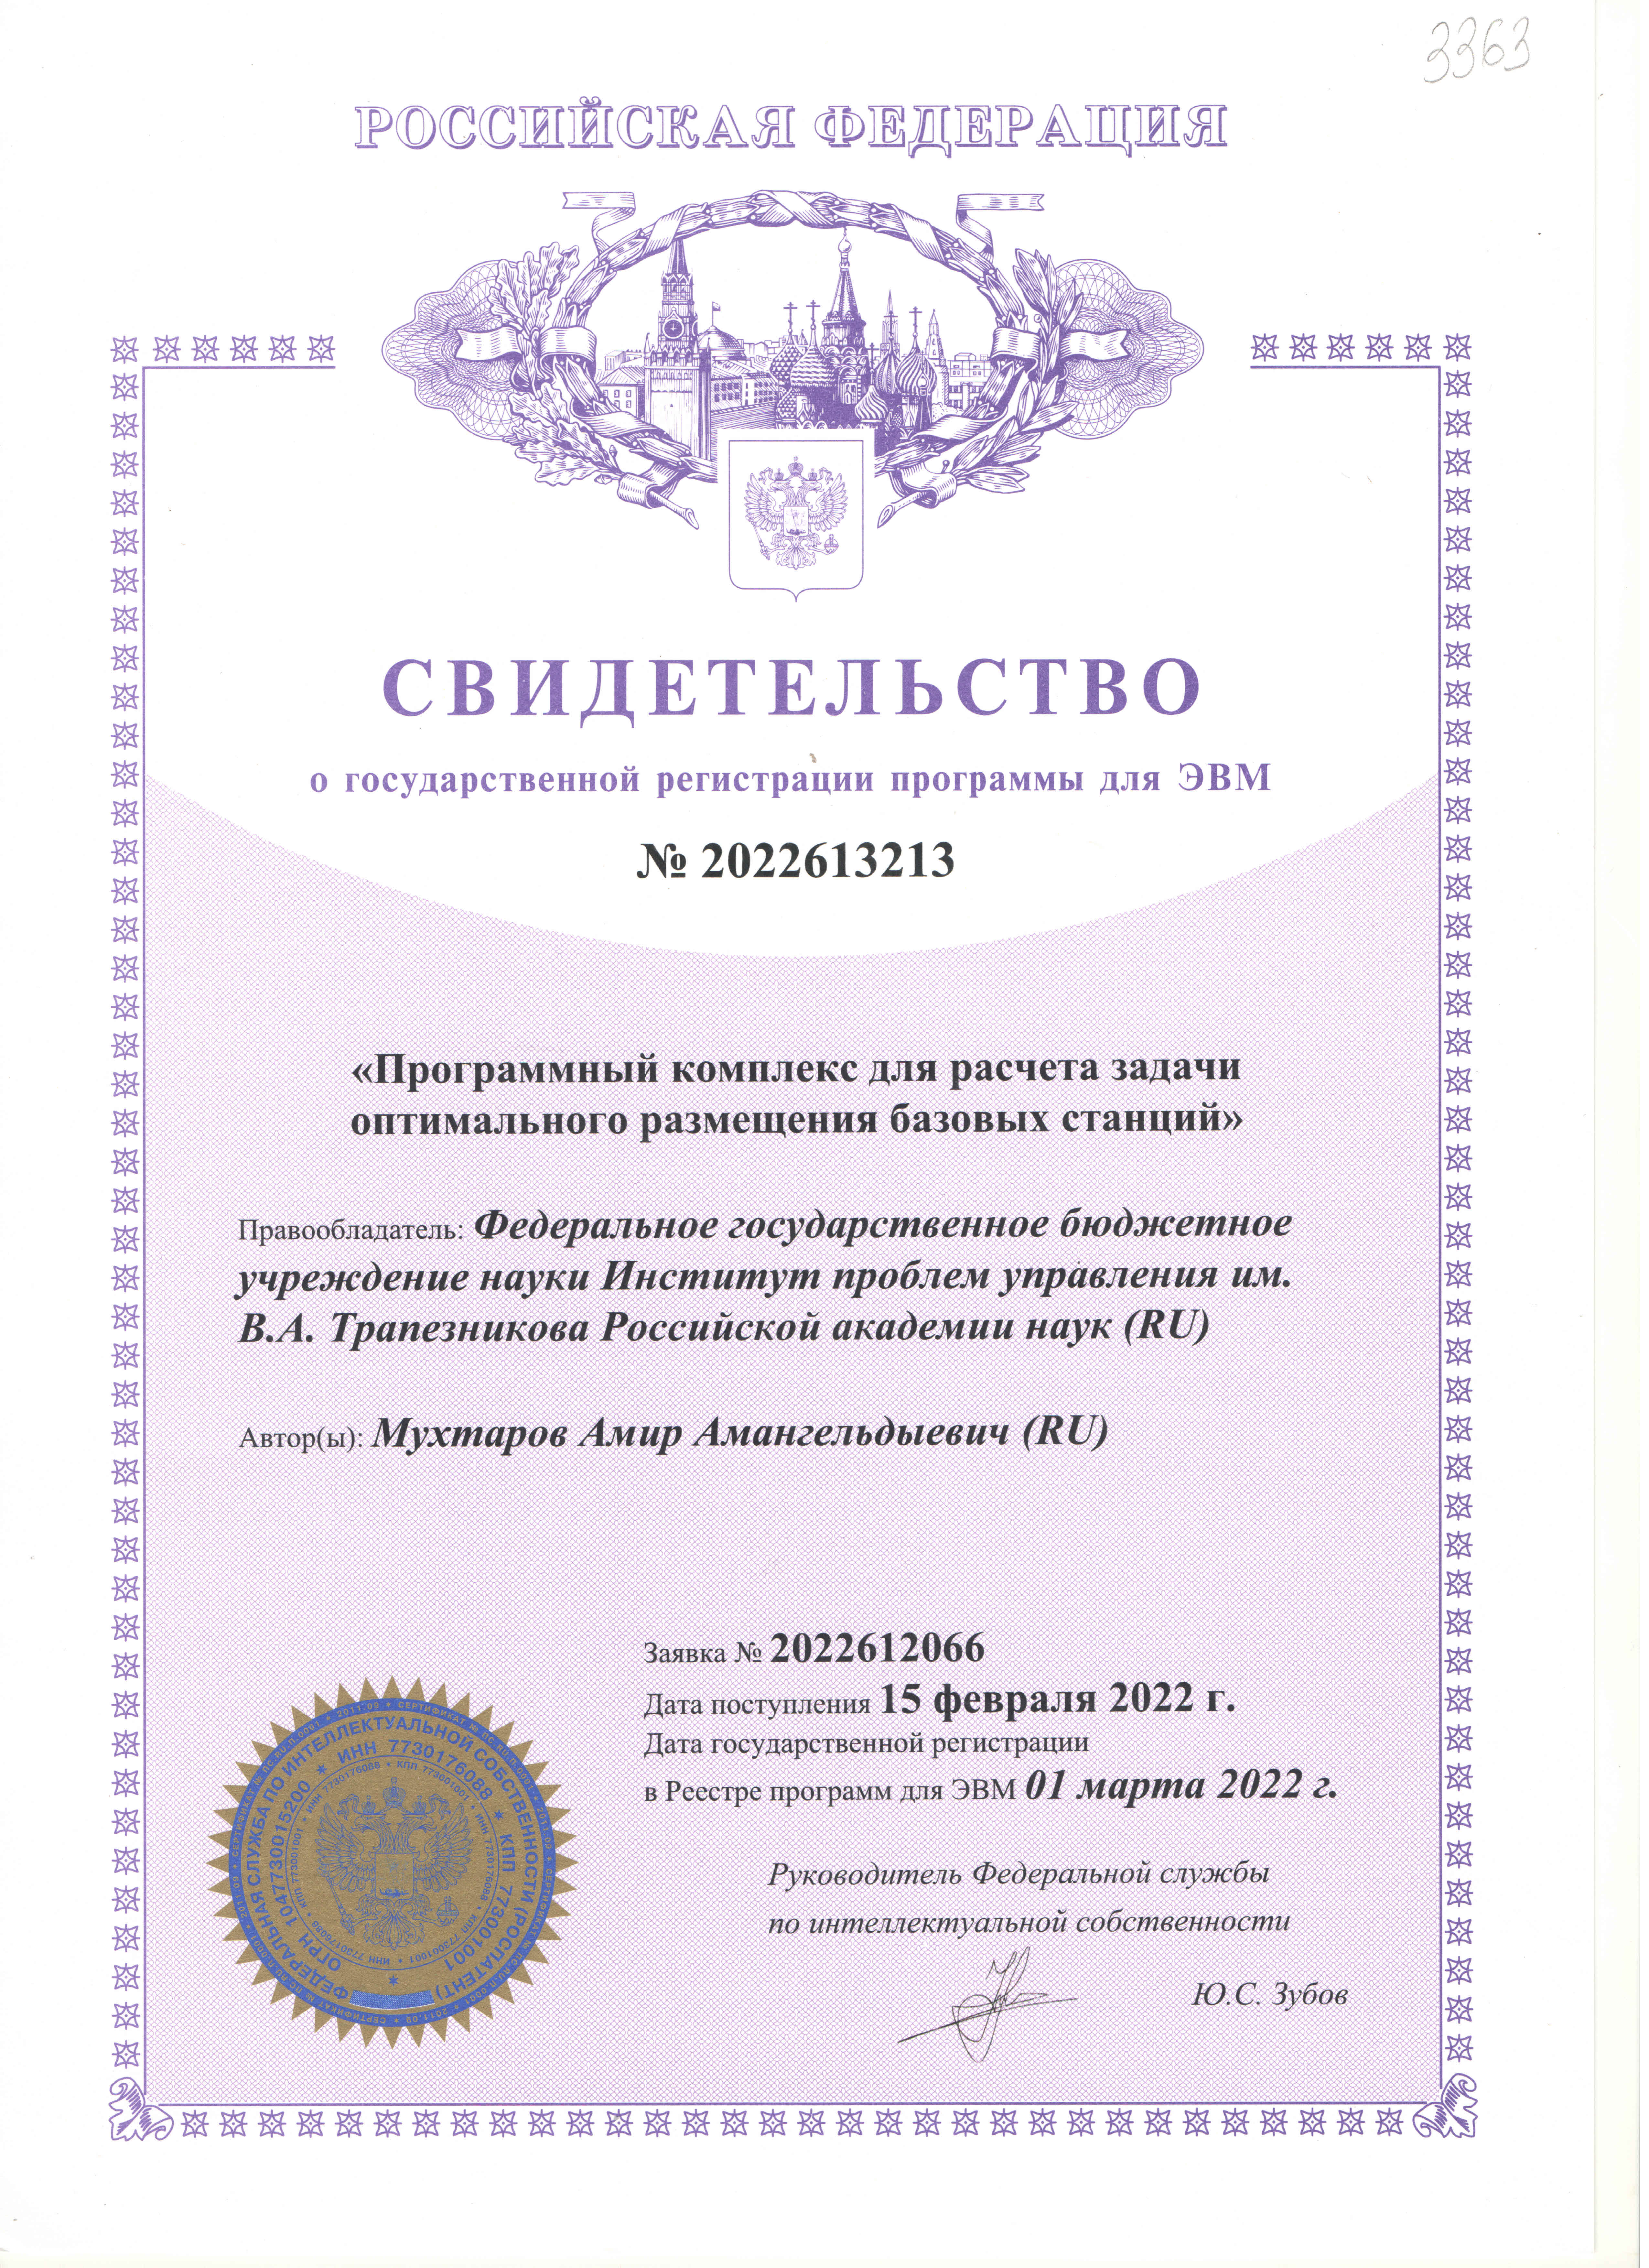
\includegraphics[scale=0.7]{program_mukhtarov.jpeg}
    }
    \label{fig:app_program_mukhtarov}
\end{figure}

\chapter{Акт о внедрении}


\begin{figure}[ht]
    \centerfloat{
        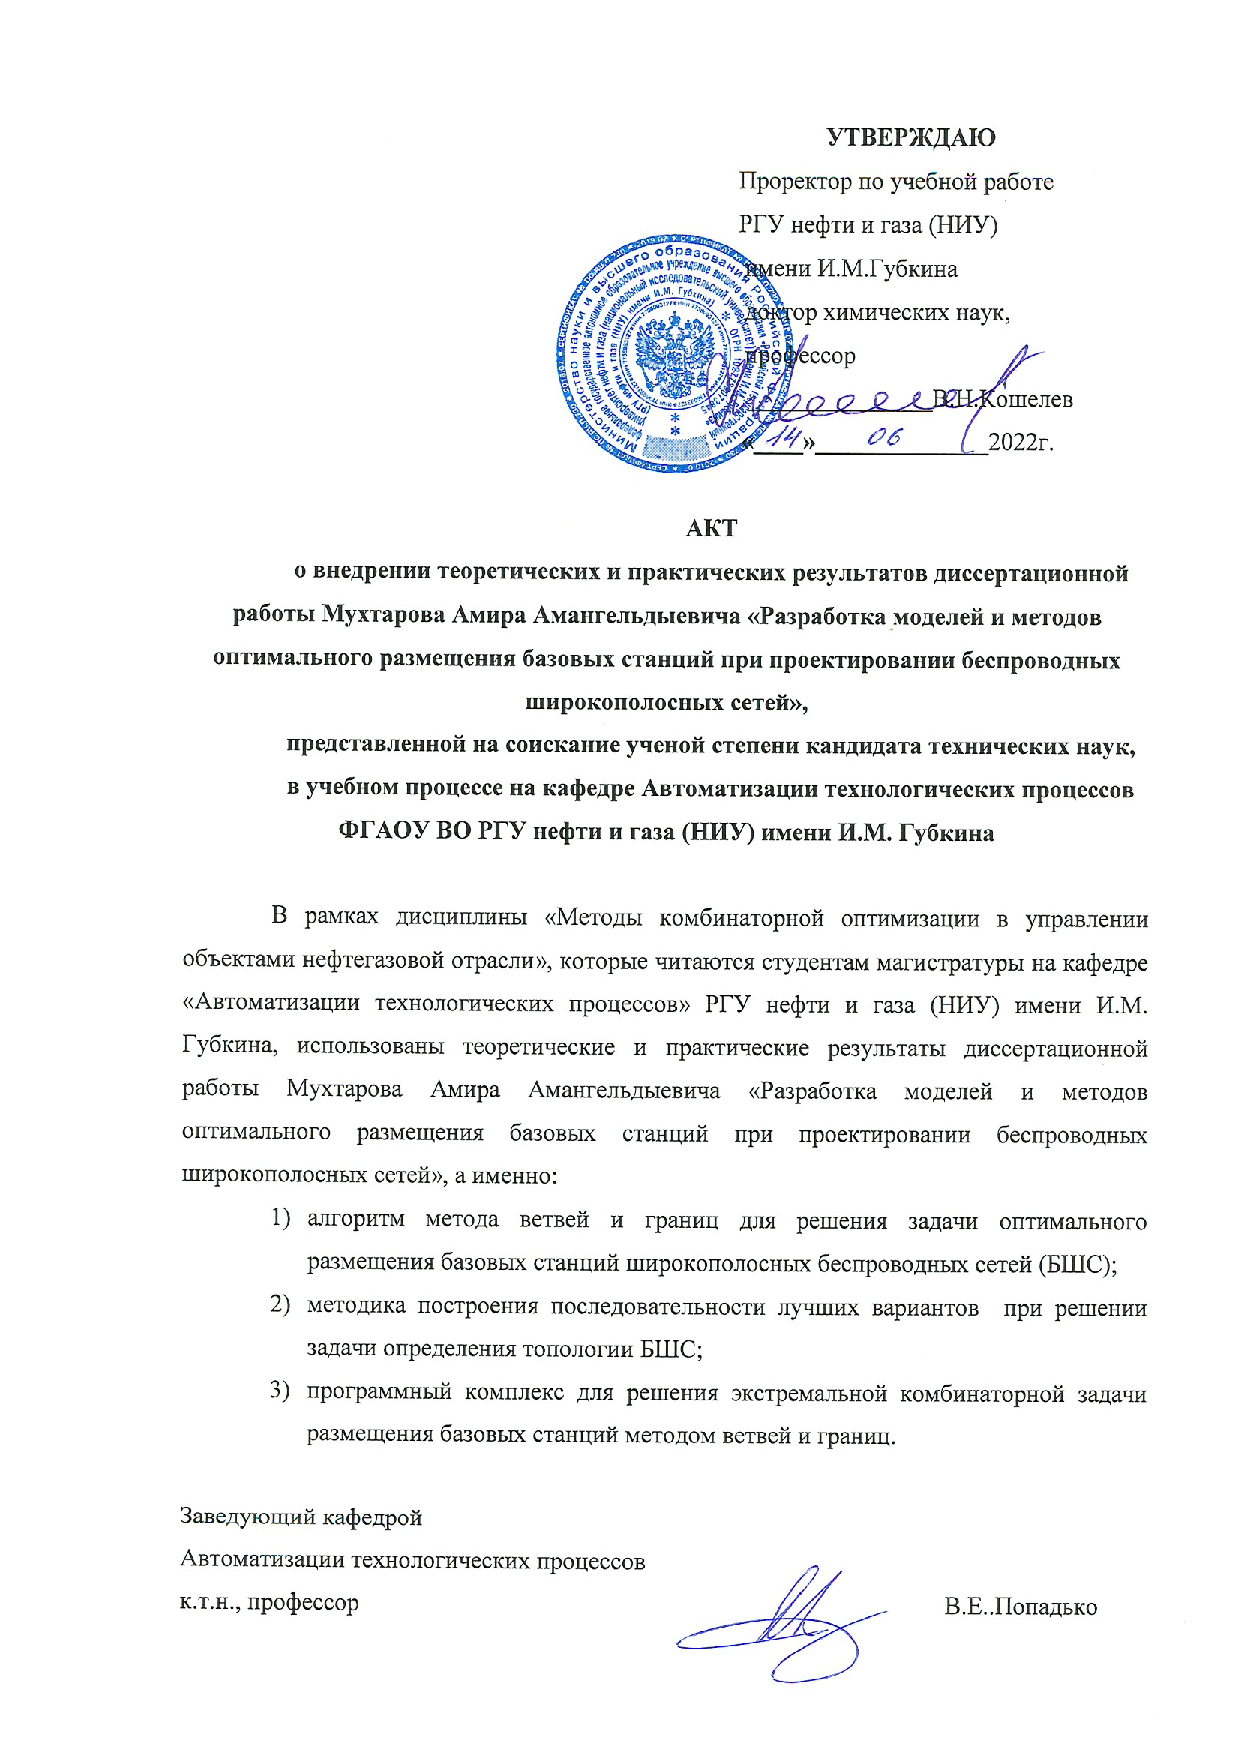
\includegraphics[scale=0.7]{implementation_act.pdf}
    }
    \label{fig:app_implementation_act_mukhtarov}
\end{figure}

% \chapter{Сравнения оценок «недопокрытия» для задачи 2, 3 и 4}\label{app:task_234}

% В таблице \cref{tab:app_estimate_comparison} приведены результаты вычислительного эксперимента, показывающего время решения \underline{\textit{\textbf{задач 2, 3, 4}}} и относительную точность \underline{\textit{\textbf{задачи 3, 4}}} по отношению к \underline{\textit{\textbf{задаче 2}}}.

% Для непокрытого участка справа длины $|\beta| = 50$, варьируя количеством неразмещенных станций, а также количеством свободных мест размещения рассчитаем оценку недопокрытия при бюджетном ограничении $C=600$.




% \fontsize{8pt}{8pt}\selectfont
% \begin{longtable}[c]{| c | c | c | c | c | c | c | c |c | c |}
%     \caption{Сравнения оценок «недопокрытия» для задачи ЦЛП и ЛП}\label{tab:app_estimate_comparison}\\

%     \hline
%     \multirow{2}{*}{\thead{Количество \\
%         точек \\
%         размещения, \\ $m$}}
%     & \multirow{2}{*}{\thead{Количество \\
%         свободных \\
%         станций, \\ $|S_\beta|$}}

%     & \multicolumn{2}{|c|}{ЦЛП} 
%     & \multicolumn{3}{|c|}{\thead{Задача \\
%     о ранце}} 
%     & \multicolumn{3}{|c|}{ЛП} \\\cline{3-10}
 
%     &&\rotatebox{270}{Время расчета, сек } 
%     &\rotatebox{270}{Недопокрытие, $z$}
%     &\rotatebox{270}{Время расчета, сек} 
%     &\rotatebox{270}{Недопокрытие, $z$}
%     &\rotatebox{270}{Точность, \%}
%     &\rotatebox{270}{Время расчета, сек} 
%     &\rotatebox{270}{Недопокрытие, $z$}
%     &\rotatebox{270}{Точность, \%}\\

%     \hline
%     5&	6&	0,3250&	436,00&	0,3214&	426,00&	97,71&	0,0047&	436,00&	100,00 \\
%     5&	8&	0,3218&	431,00&	0,3582&	398,00&	92,34&	0,0045&	431,00&	100,00 \\
%     8&	10&	0,3765&	395,00&	0,3621&	375,00&	94,94&	0,0094&	395,00&	100,00 \\
%     8&	12&	0,3746&	390,00&	0,2977&	347,00&	88,97&	0,0094&	390,00&	100,00 \\
%     12&	15&	0,3363&	339,00&	0,2960&	309,00&	91,15&	0,0114&	339,00&	100,00 \\
%     12&	17&	0,4072&	336,00&	0,3456&	283,00&	84,23&	0,0136&	336,00&	100,00 \\
%     18&	20&	0,3558&	265,00&	0,3407&	265,00&	100,00&	0,0121&	265,00&	100,00 \\
%     18&	25&	0,3794&	260,00&	0,3096&	259,00&	99,62&  0,0169&	257,60&	99,08 \\
%     25&	30&	0,3177&	246,00&	0,3576&	246,00&	100,00&	0,0222&	244,33&	99,32 \\
%     25&	45&	0,3539&	229,00&	0,3556&	229,00&	100,00&	0,0494&	226,40&	98,86 \\
%     30&	50&	0,2994&	225,00&	0.3146&	225,00&	100,00&	0,0570&	224,13&	99,61 \\
%     30&	100& 0,5179& 223,00& 0,5177& 223,00& 100,00& 0,1513& 218,75& 98,09 \\
%     \hline
% \end{longtable}
% \normalsize


% % \fontsize{8pt}{8pt}\selectfont
% % \begin{longtable}[c]{| c | c | c | c | c | c | c | c |c | c |}
% %     \caption{Сравнения оценок «недопокрытия» для задачи ЦЛП и ЛП}\label{tab:app_estimate_comparison}\\

% %     \hline
% %     \multirow{2}{*}{\thead{Количество \\
% %         точек \\
% %         размещения, \\ $m$}}
% %     & \multirow{2}{*}{\thead{Количество \\
% %         свободных \\
% %         станций, \\ $|S_\beta|$}}

% %     & \multicolumn{2}{|c|}{ЦЛП} 
% %     & \multicolumn{3}{|c|}{\thead{Задача \\
% %     о ранце}} 
% %     & \multicolumn{3}{|c|}{ЛП} \\\cline{3-10}
 
% %     &&\rotatebox{270}{Время расчета, сек } 
% %     &\rotatebox{270}{Недопокрытие, $z$}
% %     &\rotatebox{270}{Время расчета, сек} 
% %     &\rotatebox{270}{Недопокрытие, $z$}
% %     &\rotatebox{270}{Точность, \%}
% %     &\rotatebox{270}{Время расчета, сек} 
% %     &\rotatebox{270}{Недопокрытие, $z$}
% %     &\rotatebox{270}{Точность, \%}\\

% %     \hline
% %     5&	6&	0,3250&	436,00&	0,3214&	426,00&	97,71&	0,0047&	436,00&	100,00 \\
% %     5&	8&	0,3218&	431,00&	0,3582&	398,00&	92,34&	0,0045&	431,00&	100,00 \\
% %     8&	10&	0,3765&	395,00&	0,3621&	375,00&	94,94&	0,0094&	395,00&	100,00 \\
% %     8&	12&	0,3746&	390,00&	0,2977&	347,00&	88,97&	0,0094&	390,00&	100,00 \\
% %     12&	15&	0,3363&	339,00&	0,2960&	309,00&	91,15&	0,0114&	339,00&	100,00 \\
% %     12&	17&	0,4072&	336,00&	0,3456&	283,00&	84,23&	0,0136&	336,00&	100,00 \\
% %     18&	20&	0,3558&	265,00&	0,3407&	265,00&	100,00&	0,0121&	265,00&	100,00 \\
% %     18&	25&	0,3794&	260,00&	0,3096&	259,00&	99,62&  0,0169&	257,60&	99,08 \\
% %     25&	30&	0,3177&	246,00&	0,3576&	246,00&	100,00&	0,0222&	244,33&	99,32 \\
% %     25&	45&	0,3539&	229,00&	0,3556&	229,00&	100,00&	0,0494&	226,40&	98,86 \\
% %     30&	50&	0,2994&	225,00&	0.3146&	225,00&	100,00&	0,0570&	224,13&	99,61 \\
% %     30&	100& 0,5179& 223,00& 0,5177& 223,00& 100,00& 0,1513& 218,75& 98,09 \\
% %     \hline
% % \end{longtable}
% % \normalsize

% Как видно из результатов расчетов в таблице \cref{tab:app_estimate_comparison}, представляется целесообразным  использовать  \underline{\textit{\textbf{задачу 3}}} в качестве оценки $w_2 (G_\nu )$ для решения задач большой размерности, так как время ее расчета в виде задачи линейного программирования существенно ниже с учетом высокой точности.



% \chapter{Численный пример оптимального размещения базовых станций сети с линейной топологией в виде задачи целочисленного линейного программирования}\label{app:ilp_solution}
% В этой секции представлен численный пример решения данной задачи.
% % This section shows one simple case of the problem.

% Задан линейный участок $L$ с длиной 300 с количеством $n=7$ точек размещения. Координаты точек размещения представлены в таблице \cref{tab:part3_placed_point}.  Задан бюджет размещения $C=130$. Центральная частота $f = 2437$ МГц. 

% \begin{table}[h!]\centering
%   \begin{tabular}{|c||c|c|c|c|c|c|c|}\hline
%     $a_i$ & $a_1$ &  $a_2$ & $a_3$ & $a_4$ & $a_5$ & $a_6$ & $a_7$ \\ \hline \hline
%     Координата & 29 & 40 & 95 & 139 & 181 & 230 & 273 \\ \hline
% \end{tabular}\caption{Точки размещения участка с длиной $L = 300$.}\label{tab:part3_placed_point}
% \end{table}

% Задано множества базовых станций $m = 8$ с параметрами представленными в таблице \cref{tab:part3_BS}. Также в таблице представлены параметры шлюзов и контролируемых объектов. Параметры объектов необходимы для расчета радиусов покрытия станций.

% \begin{table}[b]\centering
%   \begin{tabular}{|c||c|c|c|c|c|c|c|}\hline
%     BS & $P_{tr}^R$ &  $G_{tr}^R$ & $P_{recv}^R$ & $P_{recv}^r$ & $G_{recv}^r$ & $c$ \\ \cline{2-1} \cline{3-1} \cline{4-1} \cline{5-1}  \cline{6-1} \cline{7-1}
%      & дБм & дБ & Дбм & дБм & дБ & у.е.  \\ \hline
%     1 & 20 & 5 & -69 & -67 & 5 & 40 \\ 

%     2 & 19 & 5 & -67 & -67 & 5 & 28 \\ 

%     3 & 18 & 5 & -69 & -67 & 5 & 45 \\ 

%     4 & 19 & 5 & -69 & -67 & 6 & 22 \\ 

%     5 & 19 & 5 & -67 & -67 & 5 & 21 \\ 

%     6 & 20 & 5 & -69 & -67 & 5 & 40 \\ 

%     7 & 19 & 5 & -67 & -67 & 5 & 28 \\

%     8 & 18 & 5 & -69 & -67 & 5 & 45 \\ \hline \hline  

%     &  $G_{recv}^R$ & $P_{recv}^R$ &  & & $P_{tr}^r$ & $G_{tr}^r$ \\  \cline{2-1} \cline{3-1} \cline{6-1} \cline{7-1} 

%     Шлюз& дБ & дБм & & Объект & дБм & дБ  \\  \cline{2-1} \cline{3-1}  \cline{6-1} \cline{7-1}

%     &  5 & -69 & &  & 15 & 2  \\ \hline

%   \end{tabular}\caption{Параметры базовых станций, шлюзов и объектов.}\label{tab:part3_BS} 
% \end{table}

% \textbf{Расчет радиса связи между станциями}
% Базовые станции оснащены направленной антенной с высоким коэффициентом усиления для связи с соседними станциями.
% Для расчета потерь между станциями $j$ и $q$ воспользуемся формулой (\ref{eq:part3_L_fs_from_link_budget}):

% \begin{displaymath}
%   L_{fs}^{jq} = P_{tr}^R(j) - L_{tr} + G_{tr}^R(j) + G_{tr}^R(q) - L_{recv} - SOM - P_{recv}^R(q).
% \end{displaymath}


% Потери на кабелях приемникп $ L_{recv} $ и передатчике $ L_{tr} $ примем равным 1 дБ и запас на замирания сигнала $ SOM = 10 $ дБ.

% Let us carry out an example of the calculation communication link between stations $ s_1 $ and $ s_2 $:
% Для примера расчетаем радиус связи между станциями $ s_1 $ и $ s_2 $:

% \begin{align}
%   \begin{aligned}
%   L_{fs}^{12} = P_{tr}^R(1) - L_{tr} + G_{tr}^R(1) + G_{tr}^R(2) - L_{recv} - SOM - P_{recv}^R(2)= \\
%   = 20 - 1 + 5 + 5 - 1 - 10 - (-69) = 87 (dB).
%   \end{aligned}
% \end{align}

% Для расчета канала связи необходимо использовать формулу \cref{eq:part3_D}. Несущая частота $ f = 2437 $ МГц и коэффициент для расчета потерь $ K = -27,55 $:

% \begin{align}
%   \begin{aligned}
%   R_{jq} = 10^{\left(\frac{L_{fs}^{jq} - 20\lg{F} - K}{20}\right)}
%   = 10^{\left(\frac{87 - 20\lg{2437} - (-27.55)}{20}\right)} = 174 (m).
%   \end{aligned}
% \end{align}

% В таблице \cref{tab:part3_Rjq} приведены расчеты максимальных радиусов связи между всеми станциями $ s_j $, $ j = 1, ..., m $ и шлюзом $ s_ {m + 1} $.

% \begin{table}[h!]\centering
%   \begin{tabular}{|c||c|c|c|c|c|c|c|c|c|}\hline
%       $R_{jq}$ & $s_1$ & $s_2$ & $s_3$ & $s_4$ & $s_5$ & $s_6$ & $s_7$ & $s_8$ & $s_{m+1}$ \\ \hline \hline

%       $s_1$ &--& 174& 219& 219& 174& 219& 174& 219& 219\\ 
%       $s_2$ &195& --& 195& 195& 155& 195& 155& 195& 195\\ 
%       $s_3$ &174& 138& --& 174& 138& 174& 138& 174& 174\\ 
%       $s_4$ &195& 155& 195& --& 155& 195& 155& 195& 195\\ 
%       $s_5$ &195& 155& 195& 195& --& 195& 155& 195& 195\\ 
%       $s_6$ &219& 174& 219& 219& 174& --& 174& 219& 219\\
%       $s_7$ &195& 155& 195& 195& 155& 195& --& 195& 195\\ 
%       $s_8$ &174& 138& 174& 174& 138& 174& 138& --& 174\\ 
%       \hline

% \end{tabular}\caption{Рассчитанные радиусы связи между станциями}\label{tab:part3_Rjq}
% \end{table}

% \textbf{Расчет радиуса покрытия}

% % Для покрытия заданного участка базовая станция оснащена всенаправленной антенной с выходной мощностью $ P_{tr}^r $ и усилением $ G_{tr}^r$. Потери в кабеле $ L_ {tr} $ равно 1.

% % To cover a given section, the base station is equipped with an isotropic antenna with output power $ P_ {tr} ^ r $ and gain $ G_ {tr} ^ r $ is equal to 0. The cable loss $ L_ {tr} $ is equal to 1.

% % A coverage area depends on a base station, as well as user device characteristics. Let us consider a user device with an antenna sensitivity $P_{RX} = -67$ dBm and gain $G_{RX} = 0$. Loss $L_{RX}$ is equal to 0.
% Расчет проводится аналогично расчета радиусу связи между станциями. 
% Потери в свободном простанстве для канала между $j$-ой станции и контролируемым объектом

% \begin{displaymath}
%   L_{fs}^{j} = P_{tr}^r(j) - L_{tr}  - SOM - P_{RX}. 
% \end{displaymath}


% Пример расчечта радиуса покрытия для  $1$-ой станции:

% \begin{align}
%     \begin{aligned}
%   L_{fs}^{1} = P_{tr}^r + G_{tr}^r + G_{recv}^r(1) - L_{recv}(1)  - SOM - P_{recv}^r(1) = \\
%  = 15+2+5-1-(-67)-10 = 78 \text{ (дБ)}.
%     \end{aligned}
% \end{align}

% \begin{displaymath}
%   r_{1} = 10^{\left(\frac{78 - 20\lg{2437} - (-27.55)}{20}\right)} = 77 \text{ (м)}.
% \end{displaymath}

% Рассчитанные радиусы покрытия для всех станций $ s_j $, $ j = \overline{1, m} $ представлены в таблице \cref{tab:part3_rj}).

% \begin{table}[h!]\begin{center}
%   \begin{tabular}{|c||c|c|c|c|c|c|c|c|}\hline
%       STA & $s_1$ & $s_2$ & $s_3$ & $s_4$ & $s_5$ & $s_6$ & $s_7$ & $s_8$\\ \hline \hline

%       $r_{j}$ & 77 & 77 & 77 & 87 & 77 & 77 & 77 & 77\\ \hline

% \end{tabular}\caption{Рассчитанные радиусы покрытия станций}\label{tab:part3_rj}
% \end{center}\end{table}

% Задача ЦЛП решена с помощью Optimization Toolbox MatLab. Таблица \cref{tab:part3_ilp_solution} содержит все полученные целочисленные решения.


% \begin{table}[h!]\tiny\centering
%   \begin{tabular}{|c||c|c|c|c|c|c|c||c|c|}\hline
%     $a_i$ & $a_1$ &  $a_2$ & $a_3$ & $a_4$ & $a_5$ & $a_6$ & $a_7$  & Покрытие & Цена \\ \hline 
%     Координаты & 29 & 40 & 95 & 139 & 181 & 230 & 273 & м & у.е.\\ \hline \hline
%     Целлочисленное решение 1 & $s_1$ & $s_2$ & $s_6$ & -- & -- & -- & $s_4$ & 286 & 130\\ 
%     Целлочисленное решение 2 & $s_4$ & -- & $s_5$ & $s_7$ & -- & -- & $s_2$ & 289 & 99\\
%     Оптимальное решение & $s_4$ & $s_2$ & -- & -- & $s_1$ & -- & $s_5$ & 300 & 111 \\ \hline
% \end{tabular}\caption{Решение задачи ЦЛП.}\label{tab:part3_ilp_solution}
% \end{table}

% \chapter{Метод ветвей и границ на примере задачи размещени двух базовых станций}\label{app:bnb_algorithm}

% Рассмотрим пример решения задачи в комбинаторной задачи. Пусть задан отрезок $\alpha$ длиной $L = 50$ с концами в точках $a_0$ и $a_4$ с координатами $l_0 = 0$ $l_4 = 50$. Внутри данного отрезка имеется множество точек размещения $A = \{a_i\}, i = 1, 2, 3$ с координатами $l_1 = 20, l_2 = 30, l_3 = 40$. 

% Задано множество БС $S = \{ s_j \} , j = 1, 2$. Каждой станции приписаны параметры $s_j = \{ r_j, \{R_{jq}\}\}$.  Для $s_1$ задано $r_1 = 25$, $R_{10} = 62, R_{12} = 35, R_{14} = 31$. Для $s_2$ задано $r_2 = 9$, $R_{20} = 31, R_{12} = 28, R_{24} = 39$.
% На концах отрезка размещены шлюзы $s_0$ и $s_4$. Радиус связи шлюзов для соединения с БС $R_{01} = R_{41} = 62$ и $R_{02} = R_{42} = 39$. 


% Необходимо разместить БС $s_1$ и $s_2$, т.е. найти такую расcтановку $P^*$, которая минимизирует функционал недопокрытия $f(P)$ \cref{eq:part3_objective_function}.

% \textbf{Решение полным перебором.}

% Общее количество размещения двух станций по трем точкам равна $\gamma = C^2_3 \cdot 2! = 6$.

% % Процесс решения задачи представлен в виде бинарного дерева поиска. Каждый узел пронумерован согласно правилам \textit{\textbf{процедуры 1}}. Оранжевым цветом указаны листья, в которых либо получили расстановку станций, либо на данном множестве $G_\nu$ набор фиксированных и запрещенных переменных $\pi_{ij}$ делает недопустимым любое размещение (обозначено символом $\varnothing$).

% % \fontsize{10pt}{10pt}\selectfont
% \begin{longtable}[c]{| c | c | c | c  c c|}
%     \caption{Решение полным перебором}\label{app:brute_force_solution}\\

%     \hline
%     \multirow{2}{*}{Расстановка, $P$} & \multirow{2}{*}{Недопокрытие, $f(P)$} & \multirow{2}{*}{Номер узла дерева, $\nu$} &  \multicolumn{3}{c|}{Размещение} \\\cline{4-6}

%     &&& $a_1$&	$a_2$&	$a_3$\\
%     \hline
%     $P_1$ & 11 & 3 & $S_1$ & $S_2$ & -- \\
%     $P_2$ & 1 & 5 & $S_1$ & -- & $S_2$ \\
%     $P_3$ & 11 & 9 & $S_2$ & $S_1$ & --  \\
%     $P_4$ & 11 & 11 & $S_2$ & -- & $S_1$ \\
%     $P_5$ & 6 & 15 & -- & $S_1$  & $S_2$\\
%     $P_6$ & 21 & 19 & -- & $S_2$  & $S_1$\\
%     \hline
%     \multicolumn{3}{|c|}{Количество пройденных узлов} & \multicolumn{3}{|c|}{24} \\

%     \hline
% \end{longtable}


% В таблице \cref{app:brute_force_solution} представлены полученные в ходе решения расстановки. Все расстановки пронумерованы в соответствии с порядком их нахождения. Оптимальным решением $P^*$ с минимальным значением функции \cref{eq:part3_P} является допустимая расстановка $P_2$.


% \textbf{Решение с помощью МВиГ.}

% Теперь решим пример данной задачи в соответствии с разработанным МВиГ. Так как мы не учитываем ограничения на стоимость и величину задержку, допустимая расстановка должна удовлетворять только требованию 1, а также условию размещения всех имеющихся БС.



% \textbf{Исследование множества $G_0$.}

% За начальный рекорд примем длину всего отрезка $\widehat{P} = L = 50$.

% Построение оценки $W(G_0)$:
% $$
% W(G_0)= \max\{L-2(r_1 + r_2), 0\} = \max\{50 -2(25+9), 0 \}.
% $$

% Разбиваем множества $G_0$ на два подмножества $G_1 = G^1_0$ ($\pi_{11} = 1$) и $G_2 = G^2_0$ ($\pi_{11} = 0$). Исследуем левое дочернее подмножество $G_1$. Правое подмножество $G_2$ оставим для обратного шага.

% \textbf{Исследование множества $G_1$.}

% Случай 1.

% Проверка требования 1.

% Шаг 1.

% Проверяем, что каждый из радиусов $R_{10}$ и $R_{01}$ не меньше расстояния  до левого шлюза $s_0$. 
% $$
% l_1 - l_0 \leqslant R_{10} \rightarrow 20 - 0 \leqslant 62;
% $$

% $$
% l_1 - l_0 \leqslant R_{01} \rightarrow 20 - 0 \leqslant 62;
% $$

% Шаг 2.
% Осталось неразмещенная БС $s_2$. Проверяем, что радиусы связи $R_{12}$ и $R_{21}$ не меньше расстояния до правой точки от $a_1$ точка $a_2$.
% $$
% l_2 - l_1 \leqslant R_{12} \rightarrow 30 - 20 \leqslant 35;
% $$

% $$
% l_2 - l_1 \leqslant R_{21} \rightarrow 30 - 20 \leqslant 28.
% $$

% Шаг 3.

% Так как осталась только одна нераспределенная станция $s_2$, проверяем, что расстояние среди еще незанятых точек справа от точки $a_1$  есть такая точка, что расстояния от этой точки до точки $a_1$ и одновременно от этой точки до точки $a_{n+1}$ не больше, чем  радиус связи у нераспределенной станции.

% Проверка точки $a_2$.
% $$
% l_2 - l_1 \leqslant R_{21} \rightarrow 30 - 20 \leqslant  28;
% $$

% $$
% l_4 - l_2 \leqslant R_{21} \rightarrow 50 - 20 \leqslant  31;
% $$

% Проверка точки $a_2$.
% $$
% l_3 - l_1 \leqslant R_{21} \rightarrow 40 - 20 \leqslant  28;
% $$

% $$
% l_4 - l_3 \leqslant R_{21} \rightarrow 50 - 40 \leqslant  31;
% $$

% Проверка обеспечения связи между размещаемыми БС произведена, можно приступать к оценке недопокрытия.

% Случай 2.

% Построение оценки $W(G_1)$:

% $$
% W(G_1) = w_1(G_1) + w_2(G_1).
% $$

% Недопокрытие слева от размещаемой БС $s_1$:

% $$
% w_1(G_1) = \max\{(l_1 - l_0) - r_1, 0\} \rightarrow \max\{(20 - 0) - 25, 0\} = 0.
% $$

% И оценка недопокрытия справа от размещаемой БС $s_1$: 
% $$
% w_2(G_1) = \max\{(l_4 - l_1) - (r_1 + 2r_2), 0\} \rightarrow \max\{(50 - 20) - (25 + 2 \cdot 9, 0\} = 0.
% $$

% Итоговая оценка
% $$
% W(G_1) = 0 + 0 = 0.
% $$

% Разбиваем множества $G_1$ на два подмножества $G_3 = G^1_1$ ($\pi_{22} = 1$) и $G_4 = G^2_1$ ($\pi_{22} = 0$). Исследуем  левое дочернее подмножество $G_3$. Правое подмножество $G_4$ оставим для обратного шага.

% \textbf{Исследование множества $G_3$.}

% Случай 1.

% Проверка требования 1 проводится аналогичным образом. Перейдем к расчету оценки.

% Случай 2.

% Построение оценки $W(G_3)$:

% $$
% W(G_3) = w_1(G_3) + w_2(G_3).
% $$

% Недопокрытие слева от размещаемой БС $s_2$:

% $$
% w_1(G_3) =  w_1(G_1) + (l_2 - l_1) - (r_1 + r_2) \rightarrow 0 + \max\{(30 - 20) - (25+ 9), 0\} = 0 + 0 = 0
% $$

% Оценка недопокрытия справа от размещаемой БС $s_2$: 
% $$
% w_2(G_3) = \max\{(l_4 - l_2) - r_2, 0\} \rightarrow \max\{(50 - 30) - 9, 0\} = 11.
% $$

% $$
% W(G_3) = 0 + 11 = 11.
% $$

% Все $m$ станции размещены, $f(P_1) = W(G_3)$. Так как $f(P_1) \leqslant f(\widehat{P}) \rightarrow f(P_1) \leqslant 50$, полученное недопокрытие $f(P_1)$ принимается за новый рекорд.

% Следующим этапом будет обратный шаг по дереву поиска, так как все станции размещены, то есть нет свободных переменных $\pi_{ij}$ в множестве $\Pi^f$. Незакрытая вершина с наибольшим порядковым номером -- вершина $G_4$ с условием $\pi_{22}=0$.

% \textbf{Исследование множества $G_4$.}


% Случай 2.

% Оценка правого дочернего узла $W(G_4)$ равна оценке материнского узла $W(G_1)$, $w_1(G_4)=w_1(G_1)$, $w_2(G_4) = w_2(G_1)$, и $W(G_4) = W(G_1) = 0$.


% Разбиваем множества $G_4$ на два подмножества $G_5 = G^1_4$ ($\pi_{32} = 1$) и $G_6 = G^2_4$ ($\pi_{32} = 0$).

% \textbf{Исследование множества $G_5$.}

% Случай 1. Успешная проверка требования 1.


% Случай 2.

% Построение оценки $W(G_5)$:

% $$
% W(G_5) = w_1(G_5) + w_2(G_5).
% $$

% Недопокрытие слева от размещаемой БС $s_2$:

% $$
% w_1(G_5) =  w_1(G_5) + (l_3 - l_1) - (r_1 + r_2) \rightarrow 0 + \max\{(40 - 20) - (25+ 9), 0\} = 0 + 0 = 0
% $$

% Оценка недопокрытия справа от размещаемой БС $s_2$: 
% $$
% w_2(G_5) = \max\{(l_4 - l_3) - r_2, 0\} \rightarrow \max\{(50 - 40) - 9, 0\} = 1.
% $$

% $$
% W(G_5) = 0 + 1 = 1.
% $$

% Все $m$ станции размещены, $f(P_2) = W(G_5)$. Так как $f(P_2) \leqslant f(\widehat{P})$, полученное недопокрытие $f(P_2)$ принимается за новый рекорд.



% \begin{longtable}[c]{| c | c | c | c | c  c c|}
%   \caption{Решение методом ветвей и границ}\label{app:branch_and_bound_solution}\\

%   \hline
%   \multirow{3}{*}{№}& Номер & Оценка & Недопокрытие, &  \multicolumn{3}{c|}{Размещение} \\

%   &узла & недопокрытия,& $f(P)$ & &	&	\\ \cline{5-7}
%   &дерева, $\nu$ &$W(G_\nu)$& & $a_1$&	$a_2$&	$a_3$\\
%   \hline
%   1&0 &0&50 & --&	--&	--\\
%   2&1 &0& & $s_1$ &	--&	--\\
%   3&3 &11& Рекорд & $s_1$ &	$s_2$&	--\\
%   4&4 &0&  & $s_1$ &	--&	-- \\
%   5&5 &1& Рекорд & $s_1$ &	--&	$s_2$ \\
%   6&6 & 0& $\varnothing$& $s_1$ &	--&	-- \\
%   7&2 &0& & --&	--&	--\\
%   8&7 &11& & $s_2$&	--&	--\\
%   9&8 &0& & --&	--&	--\\
%   10&9 &5& & --&	$s_1$&	--\\
%   11&10 &0& & --&	--&	--\\
%   12&11 &21& & --&	$s_2$&	--\\
%   13&12 &0& & --&	--&	--\\
%   14&13 &15& & --&	--&	$s_1$\\
%   15&14 &0& & --&	--&	--\\
%   16&15 &0& $\varnothing$& --&	--&	--\\
%   17&16 &0& & --&	--&	--\\


%   \hline
% \end{longtable}

% В ходе движения по дереву поиска исследования вершин происходило аналогичным образом как показано ранее. Оптимальным решением задачи стала расстановка $P_2$ c нелопокрытием $f(P_2) = 1$. В таблице \cref{app:branch_and_bound_solution} представлены полученные оценки в ходе движения по дереву ветвлений.  Все вершины закрыты, количество пройденных узлов бинарного дерева поиска МВиГ составляет 16.

% \chapter{Численный пример оптимального размещения базовых станций сети с линейной топологией в виде экстремальной задачи в комбинаторной форме}\label{app:bnb_solution}



% Дано:
% \begin{itemize}
%   \item линейный участок $L =300$ метров;
%   \item множество точек размещения $|A| =8$;
%   \item множество БС $|S| =8$;
%   \item протокол IEEE 802.11n;
%   \item ограничение на суммарную стоимость $T =0.001$с;
%   \item интенсивность входящих пакетов $\lambda = 1000$ 1/c;
%   \item средний размер входящих пакетов $w = 1500$ байт;
%   \item отклонение от оптимального решения, $\varepsilon=0.5$%
% \end{itemize}

% Рассмотрим пример задачи оптимального размещения базовых станций вдоль линейного участка для организации БШС. В данном приложении будет представлен пример решения на базе семейства протоколов IEEE 802.11. Задан линейный участок $L =230$ метров. На данном участке задано множество точек размещения  $|A| =6$ с координатами, представленными в таблице \cref{tab:placement_point}. Задано множество станций $|S| =5$, таблице \cref{tab:sta_parameters}. 


% % $\{36, 51, 115, 135, 182, 191\}$ метров


% Задан линейный участок $L =300$ метров. На данном участке в ходе обследования местности были выбраны восемь возможных точек размещения базовых станций, $|A| =8$. Координаты $l_i$ точек размещения представлены в таблице \cref{tab:placement_point}.

% \begin{table}[h!]\centering
%   \begin{tabular}{|c||c|c|c|c|c|c|c|c|}\hline
      
%       Точки размещения, $a_i$ &	$a_1$&	$a_2$&	$a_3$&	$a_4$&	$a_5$&	$a_6$&	$a_7$& $a_8$ \\
%       \hline
%       Координаты, $l_i$ &	43&	72&	98&	150&	178&	201&	269&	280\\
%       \hline

% \end{tabular}\caption{Координаты точек размещения}\label{tab:placement_point}
% \end{table}

% На рынке представлен широкий спектр технических устройств от компаний Cisco, Mikrotik и т.д. позволяющий организовывать сеть в открытой местности и учитывающий климатические сложности на нефтегазовых месторождениях, такие как предельные температуры, сила ветра и т.д. Под БС в нашей задаче будем понимать точку доступа с антеннами для покрытия заданной области и антеннами для обеспечения связи с соседними станциями БШС. 

% В ходе этапа выбора комплекса технических средств были выбраны восемь БС. Множество станций $|S| = 8$. Каждой БС преписаны паспортные характеристики антенн, пропускная способность точки доступа и итоговая стоимость станции. Стоимость взята условная, чтобы не указывать реальные цены производителя на время написания диссертации и курс валют. Будем рассматривать БШС для задачи мониторинга, то есть с каналом передачи на верхний уровень, UpLink. Рабочая частота 2,4 ГГц. Для каждой БС будем использовать пропускную способность для модуляции и схемы кодирования MCS7.  В таблице \cref{tab:sta_parameters} представлены параметры БС. Здесь $P_{tr}^{R}$ -- мощность направленной антенны, $G_{tr}^R$ -- усиление направленной антенны, $P_{recv}^R$ -- чувствительность направленной антенны, $L$  -- потери в антенном кабеле и разъемах, передающего тракта, $P_{recv}^r$ -- чувствительность всенаправленной антенны, $G_{recv}^r$ -- усиление всенаправленной антенны,  $p$ – пропускная способность, $c$ – стоимость


% \begin{table}[h!]\centering
%   \begin{tabular}{|c||c|c|c|c|c|c|c|c|}\hline
      
%       S&	$P_{tr}^R$&	$G_{tr}^R$&	$P_{recv}^R$&	$L$&	$P_{recv}^r$&	$G_{recv}^r$&	$p$&	$c$ \\
%       \hline
%       №&	дБм&	дБ&	дБм&	дБ&	дБм&	дБ&	Мбит/с&	у.е. \\
%       \hline
%       1&	20&	4&	-77&	1&	-77&	3&	72,2& 24 \\
%       2&	19&	4&	-77&	1&	-73&	4&	72,2&	20 \\
%       3&	19&	4&	-77&	1&	-77&	5&	72,2&	24 \\
%       4&	18&	4&	-77&	1&	-77&	3&	72,2&	24 \\
%       5&	19&	4&	-77&	1&	-77&	4&	72,2&	28 \\
%       6&	19&	4&	-77&	1&	-74&	4&	72,2&	24 \\
%       7&	20&	4&	-77&	1&	-73&	4&	72,2&	20 \\
%       8&	19&	4&	-77&	1&	-77&	4&	72,2&	20 \\
%       \hline

% \end{tabular}\caption{Параметры базовых станций}\label{tab:sta_parameters}
% \end{table}

% На концах участка размещены шлюзы $s_0 $ и $s_{m+1}$ с параметрами (таблица \cref{tab:app_gateway_parameters}):

% \begin{table}[h!]\centering
%   \begin{tabular}{|c||c|c|c|c|}\hline
      
%       Шлюз&	$P_{tr}^R$&	$G_{tr}^R$&	$P_{recv}^R$&	$L$ \\
%       \hline
%       №&	дБ&	дБ&	дБ&	дБ \\
%       \hline
%       $s_0 $&	20&	5&	-77&	1 \\
%       $s_{m+1}$&	20&	5&	-77&	1 \\
%       \hline

% \end{tabular}\caption{Параметры шлюзов}\label{tab:app_gateway_parameters}
% \end{table}

% Для расчета области покрытия необходимо задаться характеристиками устройств, с которых будет собираться информация (таблица \cref{tab:app_user_device_parameters}).


% \begin{table}[h!]\centering
%   \begin{tabular}{|c||c|c|c|}\hline
      
%     Устройство&	$P_{tr}^ud$&	$G_{tr}^ud$&	$L$ \\
%     \hline
%     &	дБ&	дБ&	дБ	 \\
%     \hline
%     &	9&	1&	0 \\

%     \hline

% \end{tabular}\caption{Параметры устройств}\label{tab:app_user_device_parameters}
% \end{table}


% Итоговое размещение БС должно удовлетворять заданным ограничениям:
% \begin{itemize}
%   \item на стоимость $C = 76$;
%   \item на межконцевую задержку сети $T =0.001$ с.
% \end{itemize}
% Для расчета времени межкоцневой задержки, будем считать, что на каждую БС поступает трафик с интенсивностью $\lambda = 1000$ 1/с. Средний размер поступающих пакетов $w=1500$ байт.

% Для поиска последовательности топологий задано отклонение $\varepsilon=0.5$\% от найденного оптимального значения.

% \subsubsection{Расчет радиуса связи и радиуса покрытия станций}

% По формуле (5) рассчитаем радиус покрытия для каждой станции (таблица \cref{tab:app_sta_coverage}) и радиусы связи между станциями и со шлюзами (таблица \cref{tab:app_sta_link} и таблица \cref{tab:app_gateway_link}).

% \begin{table}[h!]\centering
%   \begin{tabular}{|c||c c c c c c|}\hline
      
%       Станция&	$S_1$& $S_2$& $S_3$& $S_4$& $S_5$& $S_{m+1}$\\
%       \hline
%       $r_j$, м&	48&	43&	38&	43&	43&	0\\
%       \hline

% \end{tabular}\caption{Рассчитанные радиусы покрытия}\label{tab:app_sta_coverage}
% \end{table}

% \begin{table}[h!]\centering
%   \begin{tabular}{|c|c c c c c c c|}\hline
      
%       $R_{jq}$, м&	$S_1$& $S_2$& $S_3$& $S_4$& $S_5$& $S_0$& $S_{m+1}$\\
%       \hline
%       $S_1$& --&	76&	96&	96&	76&	76&	76\\
%       $S_2$& 85&	--&	85&	85&	68&	68&	68\\
%       $S_3$& 76&	60&	--&	76&	60&	60&	60\\
%       $S_4$& 85&	68&	85&	--&	68&	68&	68\\
%       $S_5$& 85&	68&	85&	85&	--&	68&	68\\

%       \hline
% \end{tabular}\caption{Рассчитанные радиусы связи базовых станций}\label{tab:app_sta_link}
% \end{table}

% \begin{table}[h!]\centering
%   \begin{tabular}{|c|c c c c c|}\hline
      
%       $R_{jq}$, м&	$S_1$& $S_2$& $S_3$& $S_4$& $S_5$ \\
%       \hline
%       $S_0$& 96&	85&	76&	85&	85\\
%       $S_{m+1}$& 96&	85&	76&	85&	85\\
%       \hline
% \end{tabular}\caption{Рассчитанные радиусы связи шлюзов}\label{tab:app_gateway_link}
% \end{table}


% В таблице \cref{tab:app_bnb_solution_result} представлены результаты решения размещения станций. Для заданной $\varepsilon=1\%$, т.е. $d=2$ был получены последовательности расстановок для \underline{\textit{\textbf{задач 2, 3 и 4}}} расчета оценок с помощью задачи ЦЛП, задачи «О ранце» и ЛП. В таблице представлены рекорды «недопокрытия», стоимости и задержки сети, а также размещения станций, число пройденных узлов дерева а и время счета.
% Задача ЦЛП и задача о ранце решались с помощью Optimization Toolbox Matlab, а задача ЛП решалась с помощью библиотеки c исходным кодом Scipy Python. Как видно из результатов оценка, полученная с помощью задачи ЛП менее точная, приходится обходить большее количество узлов для нахождения рекордов по сравнению с методом оценки «недопокрытия» с помощью \underline{\textit{\textbf{задач 2 и 3}}}. В итоге возрастает итоговое количество пройденых узлов. В свою очередь метод ЛП имеет свое преимущество, так как время счета меньше.


% \fontsize{10pt}{10pt}\selectfont
% \begin{longtable}[c]{| c | c | c | c | c  c  c  c  c  c  c|}
%     \caption{Сравнения оценок «недопокрытия» для задачи ЦЛП и ЛП}\label{tab:app_bnb_solution_result}\\

%     \hline
%     \multirow{2}{*}{№} & \multirow{2}{*}{Рекорд, м} & \multirow{2}{*}{Стоимость, у.е.} & \multirow{2}{*}{Задержка, сек} & \multicolumn{7}{|c|}{Размещение} \\\cline{5-11}

%     &&&& $a_1$&	$a_2$&	$a_3$&	$a_4$&	$a_5$&	$a_6$&	$a_7$ \\
%     \hline
%     1&	1&	65&	0,03244&	$S_1$&	-&	$S_4$&	-&	-&	$S_5$&	- \\
%     2&	1&	65&	0,03244&	$S_1$&	-&	$S_5$&	-&	-&	$S_4$&	- \\
%     3&	1&	65&	0,03244&	$S_4$&	-&	$S_1$&	-&	-&	$S_5$&	- \\
%     4&	0&	65&	0,03244&	$S_4$&	-&	$S_5$&	-&	-&	$S_1$&	- \\
%     5&	1&	65&	0,03244&	$S_5$&	-&	$S_1$&	-&	-&	$S_4$&	- \\
%     6&	0&	65&	0,03244&	$S_5$&	-&	$S_4$&	-&	-&	$S_1$&	- \\
%     7&	1&	65&	0,03244&	-&	$S_1$&	$S_4$&	-&	-&	$S_5$&	- \\
%     8&	1&	65&	0,03244&	-&	$S_1$&	$S_5$&	-&	-&	$S_4$&	- \\
%     9&	1&	65&	0,03244&	-&	$S_1$&	-&	$S_4$&	-&	$S_5$&	- \\
%     10&	0&	65&	0,03244&	-&	$S_1$&	-&	$S_4$&	-&	-&	$S_5$ \\
%     11&	1&	65&	0,03244&	-&	$S_4$&	$S_1$&	-&	-&	$S_5$&	- \\
%     12&	0&	65&	0,03244&	-&	$S_4$&	$S_5$&	-&	-&	$S_1$&	- \\
%     13&	1&	65&	0,03244&	-&	$S_4$&	-&	$S_1$&	-&	$S_5$&	- \\
%     14&	0&	65&	0,03244&	-&	$S_4$&	-&	$S_1$&	-&	-&	$S_5$ \\
%     15&	1&	65&	0,03244&	-&	$S_5$&	$S_1$&	-&	-&	$S_4$&	- \\
%     16&	0&	65&	0,03244&	-&	$S_5$&	$S_4$&	-&	-&	$S_1$&	- \\
%     \hline \hline

%     \multicolumn{2}{|c|}{\thead{Метод оценки \\ «недопокрытия» \\ справа}} & \multicolumn{3}{|c|}{ЦЛП}&	\multicolumn{3}{|c|}{Задача «О ранце»}&	\multicolumn{3}{|c|}{ЛП} \\
%     \hline  \hline
%     \multicolumn{2}{|c|}{\thead{Число \\ пройденных \\ узлов}}& \multicolumn{3}{|c|}{934}&	\multicolumn{3}{|c|}{934}&	\multicolumn{3}{|c|}{1590} \\  
%     \hline
%     \multicolumn{2}{|c|}{\thead{Время \\ счета,\\ сек}}& \multicolumn{3}{|c|}{5,412}&	\multicolumn{3}{|c|}{5,136} &	\multicolumn{3}{|c|}{3,613} \\
%     \hline

%     \hline
% \end{longtable}
% \normalsize

% % \chapter{Численный пример оптимального размещения базовых станций сети с линейной топологией в виде экстремальной задачи в комбинаторной форме}\label{app:bnb_solution}



% % Дано:
% % \begin{itemize}
% %   \item линейный участок $L =300$ метров;
% %   \item множество точек размещения $|A| =8$;
% %   \item множество БС $|S| =8$;
% %   \item протокол IEEE 802.11n;
% %   \item ограничение на суммарную стоимость $T =0.001$с;
% %   \item интенсивность входящих пакетов $\lambda = 1000$ 1/c;
% %   \item средний размер входящих пакетов $w = 1500$ байт;
% %   \item отклонение от оптимального решения, $\varepsilon=0.5$%
% % \end{itemize}

% % Рассмотрим пример задачи размещения базовых станций вдоль линейного участка для организации БШС. В данном приложении будет представлен пример решения задачи для БШС на базе протокола IEEE 802.11n. 





% % Задан линейный участок $L =300$ метров. На данном участке в ходе обследования местности были выбраны восемь возможных точек размещения базовых станций, $|A| =8$. Координаты $l_i$ точек размещения представлены в таблице \cref{tab:placement_point}.

% % \begin{table}[h!]\centering
% %   \begin{tabular}{|c||c|c|c|c|c|c|c|c|}\hline
      
% %       Точки размещения, $a_i$ &	$a_1$&	$a_2$&	$a_3$&	$a_4$&	$a_5$&	$a_6$&	$a_7$& $a_8$ \\
% %       \hline
% %       Координаты, $l_i$ &	43&	72&	98&	150&	178&	201&	269&	280\\
% %       \hline

% % \end{tabular}\caption{Координаты точек размещения}\label{tab:placement_point}
% % \end{table}

% % На рынке представлен широкий спетр технических устройств от компаний Cisco, Mikrotik и т.д. позволяющий организовывать сеть в открытой местности и учитывающий климатические сложности на нефтегазовых месторождениях, такие как предельные температуры, сила ветра и т.д. Под БС в нашей задаче будем понимать точку доступа с антеннами для покрытия заданной области и антеннами для обеспечения связи с соседними станциями БШС. 

% % В ходе этапа выбора комплекса технических средств были выбраны восемь БС. Множество станций $|S| = 8$. Каждой БС преписаны паспортные характеристики антенн, пропускная способность точки доступа и итоговая стоимость станции. Стоимость взята условная, чтобы не указывать реальные цены производителя на время написания диссертации и курс валют. Будем рассматривать БШС для задачи мониторинга, то есть с каналом передачи на верхний уровень, UpLink. Рабочая частота 2,4 ГГц. Для каждой БС будем использовать пропускную способность для модуляции и схемы кодирования MCS7.  В таблице \cref{tab:sta_parameters} представлены параметры БС. Здесь $P_{tr}^{R}$ -- мощность направленной антенны, $G_{tr}^R$ -- усиление направленной антенны, $P_{recv}^R$ -- чувствительность направленной антенны, $L$  -- потери в антенном кабеле и разъемах, передающего тракта, $P_{recv}^r$ -- чувствительность всенаправленной антенны, $G_{recv}^r$ -- усиление всенаправленной антенны,  $p$ – пропускная способность, $c$ – стоимость


% % \begin{table}[h!]\centering
% %   \begin{tabular}{|c||c|c|c|c|c|c|c|c|}\hline
      
% %       S&	$P_{tr}^R$&	$G_{tr}^R$&	$P_{recv}^R$&	$L$&	$P_{recv}^r$&	$G_{recv}^r$&	$p$&	$c$ \\
% %       \hline
% %       №&	дБм&	дБ&	дБм&	дБ&	дБм&	дБ&	Мбит/с&	у.е. \\
% %       \hline
% %       1&	20&	4&	-77&	1&	-77&	3&	72,2& 24 \\
% %       2&	19&	4&	-77&	1&	-73&	4&	72,2&	20 \\
% %       3&	19&	4&	-77&	1&	-77&	5&	72,2&	24 \\
% %       4&	18&	4&	-77&	1&	-77&	3&	72,2&	24 \\
% %       5&	19&	4&	-77&	1&	-77&	4&	72,2&	28 \\
% %       6&	19&	4&	-77&	1&	-74&	4&	72,2&	24 \\
% %       7&	20&	4&	-77&	1&	-73&	4&	72,2&	20 \\
% %       8&	19&	4&	-77&	1&	-77&	4&	72,2&	20 \\
% %       \hline

% % \end{tabular}\caption{Параметры базовых станций}\label{tab:sta_parameters}
% % \end{table}

% % На концах участка размещены шлюзы $s_0 $ и $s_{m+1}$ с параметрами (таблица \cref{tab:app_gateway_parameters}):

% % \begin{table}[h!]\centering
% %   \begin{tabular}{|c||c|c|c|c|}\hline
      
% %       Шлюз&	$P_{tr}^R$&	$G_{tr}^R$&	$P_{recv}^R$&	$L$ \\
% %       \hline
% %       №&	дБ&	дБ&	дБ&	дБ \\
% %       \hline
% %       $s_0 $&	20&	5&	-77&	1 \\
% %       $s_{m+1}$&	20&	5&	-77&	1 \\
% %       \hline

% % \end{tabular}\caption{Параметры шлюзов}\label{tab:app_gateway_parameters}
% % \end{table}

% % Для расчета области покрытия необходимо задаться характеристиками устройств, с которых будет собираться информация (таблица \cref{tab:app_user_device_parameters}).


% % \begin{table}[h!]\centering
% %   \begin{tabular}{|c||c|c|c|}\hline
      
% %     Устройство&	$P_{tr}^ud$&	$G_{tr}^ud$&	$L$ \\
% %     \hline
% %     &	дБ&	дБ&	дБ	 \\
% %     \hline
% %     &	9&	1&	0 \\

% %     \hline

% % \end{tabular}\caption{Параметры устройств}\label{tab:app_user_device_parameters}
% % \end{table}


% % Итоговое размещение БС должно удовлетворять заданным ограничениям:
% % \begin{itemize}
% %   \item на стоимость $C = 76$;
% %   \item на межконцевую задержку сети $T =0.001$ с.
% % \end{itemize}
% % Для расчета времени межкоцневой задержки, будем считать, что на каждую БС поступает трафик с интенсивностью $\lambda = 1000$ 1/с. Средний размер поступающих пакетов $w=1500$ байт.

% % Для поиска последовательности топологий задано отклонение $\varepsilon=0.5$\% от найденного оптимального значения.

% % \subsubsection{Расчет радиуса связи и радиуса покрытия станций}

% % По формуле (5) рассчитаем радиус покрытия для каждой станции (таблица \cref{tab:app_sta_coverage}) и радиусы связи между станциями и со шлюзами (таблица \cref{tab:app_sta_link} и таблица \cref{tab:app_gateway_link}).

% % \begin{table}[h!]\centering
% %   \begin{tabular}{|c||c c c c c c|}\hline
      
% %       Станция&	$S_1$& $S_2$& $S_3$& $S_4$& $S_5$& $S_{m+1}$\\
% %       \hline
% %       $r_j$, м&	48&	43&	38&	43&	43&	0\\
% %       \hline

% % \end{tabular}\caption{Рассчитанные радиусы покрытия}\label{tab:app_sta_coverage}
% % \end{table}

% % \begin{table}[h!]\centering
% %   \begin{tabular}{|c|c c c c c c c|}\hline
      
% %       $R_{jq}$, м&	$S_1$& $S_2$& $S_3$& $S_4$& $S_5$& $S_0$& $S_{m+1}$\\
% %       \hline
% %       $S_1$& --&	76&	96&	96&	76&	76&	76\\
% %       $S_2$& 85&	--&	85&	85&	68&	68&	68\\
% %       $S_3$& 76&	60&	--&	76&	60&	60&	60\\
% %       $S_4$& 85&	68&	85&	--&	68&	68&	68\\
% %       $S_5$& 85&	68&	85&	85&	--&	68&	68\\

% %       \hline
% % \end{tabular}\caption{Рассчитанные радиусы связи базовых станций}\label{tab:app_sta_link}
% % \end{table}

% % \begin{table}[h!]\centering
% %   \begin{tabular}{|c|c c c c c|}\hline
      
% %       $R_{jq}$, м&	$S_1$& $S_2$& $S_3$& $S_4$& $S_5$ \\
% %       \hline
% %       $S_0$& 96&	85&	76&	85&	85\\
% %       $S_{m+1}$& 96&	85&	76&	85&	85\\
% %       \hline
% % \end{tabular}\caption{Рассчитанные радиусы связи шлюзов}\label{tab:app_gateway_link}
% % \end{table}


% % В таблице \cref{tab:app_bnb_solution_result} представлены результаты решения размещения станций. Для заданной $\varepsilon=1\%$, т.е. $d=2$ был получены последовательности расстановок для \underline{\textit{\textbf{задач 2, 3 и 4}}} расчета оценок с помощью задачи ЦЛП, задачи «О ранце» и ЛП. В таблице представлены рекорды «недопокрытия», стоимости и задержки сети, а также размещения станций, число пройденных узлов дерева а и время счета.
% % Задача ЦЛП и задача о ранце решались с помощью Optimization Toolbox Matlab, а задача ЛП решалась с помощью библиотеки c исходным кодом Scipy Python. Как видно из результатов оценка, полученная с помощью задачи ЛП менее точная, приходится обходить большее количество узлов для нахождения рекордов по сравнению с методом оценки «недопокрытия» с помощью \underline{\textit{\textbf{задач 2 и 3}}}. В итоге возрастает итоговое количество пройденых узлов. В свою очередь метод ЛП имеет свое преимущество, так как время счета меньше.


% % \fontsize{10pt}{10pt}\selectfont
% % \begin{longtable}[c]{| c | c | c | c | c  c  c  c  c  c  c|}
% %     \caption{Сравнения оценок «недопокрытия» для задачи ЦЛП и ЛП}\label{tab:app_bnb_solution_result}\\

% %     \hline
% %     \multirow{2}{*}{№} & \multirow{2}{*}{Рекорд, м} & \multirow{2}{*}{Стоимость, у.е.} & \multirow{2}{*}{Задержка, сек} & \multicolumn{7}{|c|}{Размещение} \\\cline{5-11}

% %     &&&& $a_1$&	$a_2$&	$a_3$&	$a_4$&	$a_5$&	$a_6$&	$a_7$ \\
% %     \hline
% %     1&	1&	65&	0,03244&	$S_1$&	-&	$S_4$&	-&	-&	$S_5$&	- \\
% %     2&	1&	65&	0,03244&	$S_1$&	-&	$S_5$&	-&	-&	$S_4$&	- \\
% %     3&	1&	65&	0,03244&	$S_4$&	-&	$S_1$&	-&	-&	$S_5$&	- \\
% %     4&	0&	65&	0,03244&	$S_4$&	-&	$S_5$&	-&	-&	$S_1$&	- \\
% %     5&	1&	65&	0,03244&	$S_5$&	-&	$S_1$&	-&	-&	$S_4$&	- \\
% %     6&	0&	65&	0,03244&	$S_5$&	-&	$S_4$&	-&	-&	$S_1$&	- \\
% %     7&	1&	65&	0,03244&	-&	$S_1$&	$S_4$&	-&	-&	$S_5$&	- \\
% %     8&	1&	65&	0,03244&	-&	$S_1$&	$S_5$&	-&	-&	$S_4$&	- \\
% %     9&	1&	65&	0,03244&	-&	$S_1$&	-&	$S_4$&	-&	$S_5$&	- \\
% %     10&	0&	65&	0,03244&	-&	$S_1$&	-&	$S_4$&	-&	-&	$S_5$ \\
% %     11&	1&	65&	0,03244&	-&	$S_4$&	$S_1$&	-&	-&	$S_5$&	- \\
% %     12&	0&	65&	0,03244&	-&	$S_4$&	$S_5$&	-&	-&	$S_1$&	- \\
% %     13&	1&	65&	0,03244&	-&	$S_4$&	-&	$S_1$&	-&	$S_5$&	- \\
% %     14&	0&	65&	0,03244&	-&	$S_4$&	-&	$S_1$&	-&	-&	$S_5$ \\
% %     15&	1&	65&	0,03244&	-&	$S_5$&	$S_1$&	-&	-&	$S_4$&	- \\
% %     16&	0&	65&	0,03244&	-&	$S_5$&	$S_4$&	-&	-&	$S_1$&	- \\
% %     \hline \hline

% %     \multicolumn{2}{|c|}{\thead{Метод оценки \\ «недопокрытия» \\ справа}} & \multicolumn{3}{|c|}{ЦЛП}&	\multicolumn{3}{|c|}{Задача «О ранце»}&	\multicolumn{3}{|c|}{ЛП} \\
% %     \hline  \hline
% %     \multicolumn{2}{|c|}{\thead{Число \\ пройденных \\ узлов}}& \multicolumn{3}{|c|}{934}&	\multicolumn{3}{|c|}{934}&	\multicolumn{3}{|c|}{1590} \\  
% %     \hline
% %     \multicolumn{2}{|c|}{\thead{Время \\ счета,\\ сек}}& \multicolumn{3}{|c|}{5,412}&	\multicolumn{3}{|c|}{5,136} &	\multicolumn{3}{|c|}{3,613} \\
% %     \hline

% %     \hline
% % \end{longtable}
% % \normalsize

% % \chapter{Численный пример оптимального размещения базовых станций для обслуживания заданного множества рассредоточенных объектов}\label{app:milp_place_solution}
% % Рассмотрим пример для оптимизационной задачи выбора набора размещаемых станций и определения мест их размещения.
% % Задано множество рассредоточенных объектов $A_1$, $|A_1| = 4$ и шлюз (таблица \cref{tab:part2_placement_coordinates}).

% % \begin{table}
% %     \centering
% %     \captionsetup{justification=centering} % выравнивание подписи по-центру
% %     \caption{Координаты размещения}\label{tab:part2_placement_coordinates}
% %     \begin{tabular}{|l|c|c|}
% %         \toprule
% %         0   & (7,4) & \textbf{Координаты шлюза} \\
% %         \midrule
% %         1   & (1, 5)& \textbf{Координаты объектов}  \\
% %         2   & (4.5, 4) & \\
% %         3   & (6, 3) & \\
% %         4   & (3.5, 5) & \\
% %         \midrule
% %         5   & (2, 4) & \textbf{Координаты размещения станций}  \\
% %         6   & (5, 5) & \\
% %         7   & (2, 6) & \\
% %         8   & (6, 5.5) & \\
% %         \bottomrule
% %     \end{tabular}
% % \end{table}

% % Задано множество $A_2$ возможных мест расположения станций, $|A_2| = 4$. Все вершины представлены на Рисунке \ref{fig:part2_coordinates}.
 
% % \begin{figure}[ht]
% %     \centerfloat{
% %         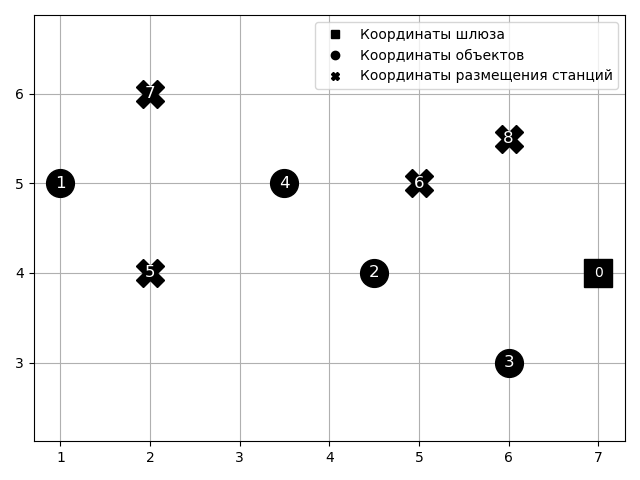
\includegraphics[scale=0.75]{part2_coordinates.png}
% %     }
% %     \caption{Координаты размещения}\label{fig:part2_coordinates}
% % \end{figure}

% % Задано ограничение по мощности для кадого объекта (таблица \ref{tab:part2_object_capacity}).

% % \begin{table}
% %     \centering
% %     \captionsetup{justification=centering} % выравнивание подписи по-центру
% %     \caption{Координаты размещения}\label{tab:part2_object_capacity}
% %     \begin{tabular}{|c|cccc|}
% %         \toprule
% %         Объекты   & 1 & 2 & 3 & 4 \\
% %         \midrule
% %         Мощность  & 10 & 15 & 17 & 18 \\
% %         \bottomrule
% %     \end{tabular}
% % \end{table}

% % Задано множество типов станций (таблица \ref{tab:part2_station_types_1}).

% % \begin{table}
% %     \centering
% %     \captionsetup{justification=centering} % выравнивание подписи по-центру
% %     \caption{Множество типов станций}\label{tab:part2_station_types_1}
% %     \begin{tabular}{|c|c|c|c|c|}
% %         \toprule
% %         Тип & Мощность, $\vartheta_j$ & Радиус покрытия, $r_j$  & Радиус связи, $R_j$ & Стоимость, $c_j$ \\
% %         \toprule
% %         1   & 80 & 1 & 6 & 70 \\
% %         2  & 100 & 2 & 5 & 75 \\
% %         3  & 100 & 2 & 5 & 75 \\
% %         \bottomrule
% %     \end{tabular}
% % \end{table}

% % Необходимо разместить станции таким образом, чтобы минимизировать их  суммарную общую стоимость.
% % Построим граф сети $H$ для данного набора типов станции. Матрица смежности представлена на рисунке \cref{fig:part2_adjacency_matrix}
 
% % \begin{figure}[ht]
% %     \centerfloat{
% %         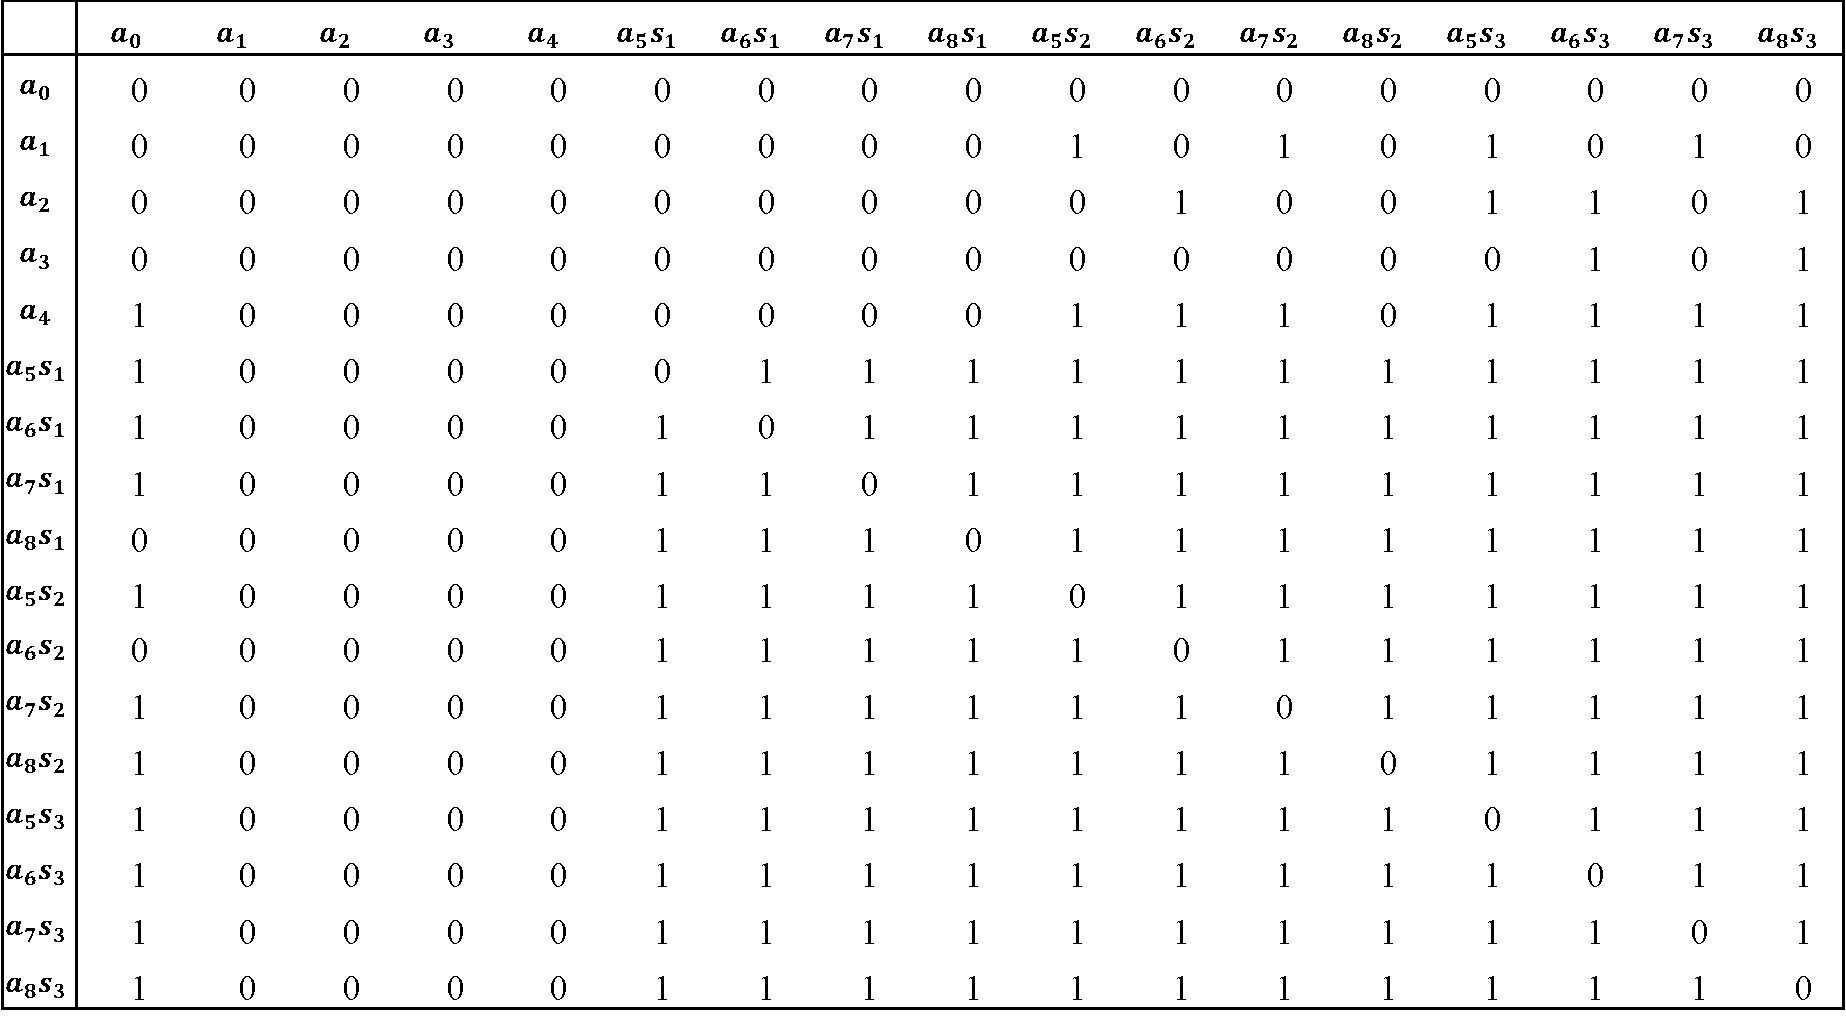
\includegraphics[scale=0.5]{part2_adjacency_matrix.pdf}
% %     }
% %     \caption{Координаты размещения}\label{fig:part2_adjacency_matrix}
% % \end{figure}

% % % \begin{table}
% % %     \centering
% % %     \captionsetup{justification=centering} % выравнивание подписи по-центру
% % %     \caption{Матрица смежности графа $H$}\label{tab:part2_adjacency_matrix}
% % %     \begin{tabular}{|c|c|c|c|c|c|c|c|c|c|c|c|c|c|c|c|c|}
% % %         \toprule
% % %         a_0 & a_1 & a_2 & a_3 & a_4 & a_5s_1 & a_6s_1 & a_7s_1 & a_8s_1 & a_5s_2 a_6s_2 & a_7s_2 & a_8s_2 & a_5s_3 & a_6s_3 & a_7s_3 & a_8s_3 \\
% % %         \toprule
% % %         1   & 80 & 1 & 6 & 70 \\
% % %         2  & 100 & 2 & 5 & 75 \\
% % %         3  & 100 & 2 & 5 & 75 \\
% % %         \bottomrule
% % %     \end{tabular}
% % % \end{table}


% % На основе матрицы смежности полученного графа запишем систему равенств и неравенств\cref{eq:part2_1.5, eq:part2_1.6, eq:part2_1.7, eq:part2_1.8, eq:part2_1.9, eq:part2_1.10} и решим задачу частично целочисленного ЛП.
% % В ходе решения мы получили следующее размещение станции (Рисунок \cref{fig:part2_solution})

% % \begin{figure}[ht]
% %     \centerfloat{
% %         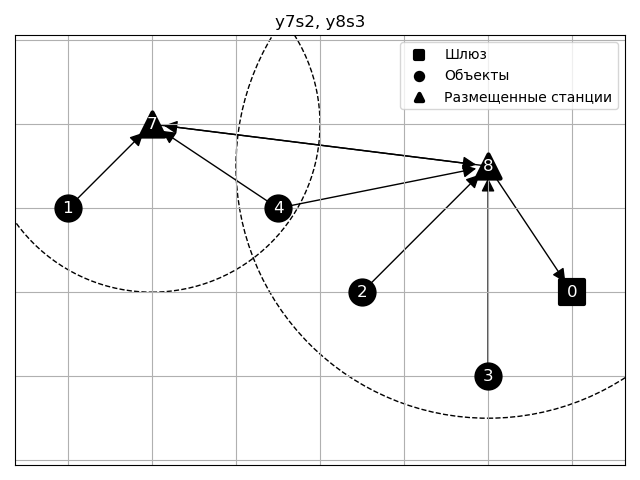
\includegraphics[scale=0.75]{part2_solution.png}
% %     }
% %     \caption{Координаты размещения}\label{fig:part2_solution}
% % \end{figure}

% % Из графика видно, что были размещены на точках 7 и 8 две станции типа 2 и 3, соответственно.
% % Решением задачи является суммарная стоимость равная:
% % $f=160$.





% % % \section{Результаты численного эксперимента}

% % Алгоритмы построения графов $H$ были запрограммированы на языке Python. Задачи, сформулированные на основании графов $H$ в виде соответствующих задач математического программирования, были решены пакетом Optimization Toolbox MATLAB.
% % В таблице 4 представлены результаты времени счета задач частично целочисленного ЛП для различных случаев числа мест размещения станций и числа объектов. Для каждого случая было проведено по 10 примеров.

% % \begin{table}
% %     \centering
% %     \captionsetup{justification=centering} % выравнивание подписи по-центру
% %     \caption{Множество типов станций}\label{tab:part2_station_types}
% %     \begin{tabular}{|c|c|c|}
% %         \toprule
% %         Количество & Количество мест  & Среднее время 
% %         \tabularnewline объектов, $n_1$ & размещения станций, $n-n_1$ &  счета, сек.  \\
% %         \toprule
% %         4   & 3 & 12,34 \\
% %         4   & 4 & 12,42 \\
% %         4   & 5 & 12,31 \\
% %         6   & 6 & 11,20 \\
% %         8   & 7 & 11,27 \\
% %         10  & 7 & 12,32 \\
% %         12  & 10 & 12,51 \\
% %         14  & 7 & 12,42 \\
% %         17  & 8 & 12,18 \\
% %         21  & 8 & 12,53 \\
% %         25  & 8 & 14,22 \\
% %         \bottomrule
% %     \end{tabular}
% % \end{table}

        % Приложения

\setcounter{totalappendix}{\value{chapter}} % Подсчёт количества приложений

\end{document}
